\documentclass[11pt]{article}

\usepackage[margin=1in]{geometry}
\usepackage[T1]{fontenc}
\usepackage{amsmath}
\usepackage{booktabs}
\usepackage{longtable}
\usepackage{pdflscape}
\usepackage[table]{xcolor}
\definecolor{loss}{HTML}{2A78D6}  % shading of the loss cells in the summary tables
\usepackage{graphicx}
\usepackage[hidelinks]{hyperref}

\title{Quantization Damage in Low-Resource Languages}
\author{Adrian Castillo}
\date{Fall 2026}

\begin{document}
\emergencystretch=3em

\maketitle

\section{Experimental Setup}

\paragraph{Research question.} Why does post-training quantization remove more of a multilingual LLM's ability to predict the next word in low-resource languages than in high-resource languages?

\paragraph{H1, under-fitted languages.} The model's weights are tuned for its training data as a whole, which is mostly high-resource text. A language it saw little of is fitted less well: the weights are roughly right for it but not quite, so its loss is still sensitive to small changes. Rounding moves every weight by about the same small amount, and that move costs more for a language whose fit was already loose (Tran et al., 2022, Zeng et al., 2024). If H1 is true, how sensitive each language's loss is to small weight changes should predict how much it loses, and in a model where we set how much text each language gets, the languages with less text should lose more.

\paragraph{H2, where the damage lives.} Rounding error is not spread evenly across the model. It concentrates in a few places, such as certain layers, a small set of unusually large weights, and the few internal dimensions that encode which language is being read (Chang, 2025, An et al., 2025, Zhong et al., 2025). If low-resource languages rely more on those places, they lose more. If H2 is true, rounding one part of the model at a time should show each language's loss coming from different parts, or from the same parts to different degrees, and restoring those parts to full precision should recover the low-resource loss.

\paragraph{Null hypothesis.} The gap is not about the language at all. It comes from the choice of model, quantization method, bit width, metric, and the random sample used to calibrate the quantization. Published studies measure damage in many different ways and none repeats its runs, and changing the calibration sample alone moves results by as much as many reported gaps (Williams et al., 2024). If the null is true, the language difference at 4 bits stays within that noise across repeated calibration samples and two model families, and H1 and H2 can only be studied at 3 bits.

\paragraph{Models.} We evaluate two base (not instruction-tuned) models: Llama 3.1 8B (\nolinkurl{meta-llama/Llama-3.1-8B}, Grattafiori et al., 2024), our core model, and Qwen 2.5 7B (\nolinkurl{Qwen/Qwen2.5-7B}, Qwen Team, 2024), a second model family used to check that results are not specific to Llama. We also evaluate a LoRA fine-tune of Llama 3.1 8B on the project language. The quantization code was developed and tested on GPT-2 small (\nolinkurl{openai-community/gpt2}, Radford et al., 2019).

\paragraph{Quantization.} We apply weight-only post-training quantization at 4 and 3 bits to every linear layer in the decoder blocks. Embeddings, \texttt{lm\_head} and normalization layers stay in bf16, and activations are not quantized. Weights use an asymmetric uniform grid with one scale and zero-point per group of 128 consecutive input columns within each row. We compare three methods. Round-to-nearest (RTN) applies the grid directly and needs no calibration. GPTQ (Frantar et al., 2023) runs in natural column order, without act-order. AWQ (Lin et al., 2024) searches the activation-aware scale per linear layer and divides it back into the weights, without the clipping search.
GPTQ and AWQ are calibrated on 128 windows of 2,048 tokens, each from a random position in a random English C4 document (Raffel et al., 2020). For Llama each window is preceded by the BOS token, as at inference (Qwen has none). GPTQ and AWQ are each run with five calibration seeds (0–4) that draw different windows, and the spread across seeds is our noise baseline. RTN needs no calibration and is run once. Each model therefore has 11 quantized versions per bit width (1 RTN + 5 GPTQ + 5 AWQ), 22 across 4 and 3 bits. With its full-precision original, each of the three models (Llama, Qwen, Llama + LoRA) has 23 versions, and all 69 are evaluated on the same test sets. 
We simulate quantization (fake quantization): weights are rounded to the grid and stored back in bf16. Since weight-only kernels dequantize weights to 16-bit before the matrix product, this produces the same outputs as packed inference. We do not measure memory or speed. As a check on our implementations, we report perplexity on the WikiText-2 test set (raw v1, Merity et al., 2017) over non-overlapping 2,048-token windows.

\begin{table}[htbp]
\centering
\small
\resizebox{\textwidth}{!}{%
\begin{tabular}{lrrrrrrr}
\toprule
Model & FP & RTN 4 & GPTQ 4 & AWQ 4 & RTN 3 & GPTQ 3 & AWQ 3 \\
\midrule
Llama 3.1 8B & 6.24 & 6.93 & 7.18 $\pm$ 0.03 & 6.65 $\pm$ 0.01 & 14.98 & 22.81 $\pm$ 2.84 & 8.61 $\pm$ 0.03 \\
Qwen 2.5 7B & 6.85 & 7.21 & 7.11 $\pm$ 0.02 & 7.10 $\pm$ 0.01 & 8.98 & 8.19 $\pm$ 0.05 & 8.32 $\pm$ 0.01 \\
Llama 3.1 8B + LoRA & 8.84 & 9.94 & 10.27 $\pm$ 0.05 & 9.42 $\pm$ 0.03 & 22.04 & 34.12 $\pm$ 7.26 & 12.15 $\pm$ 0.06 \\
\bottomrule
\end{tabular}}
\caption{WikiText-2 test perplexity (lower is better). FP is the full-precision model. GPTQ and AWQ show the mean $\pm$ standard deviation over the five calibration seeds. FP and RTN are run once.}
\end{table}

\paragraph{Languages.} English is the anchor and the other side of every translation pair. The other twelve languages fall into three groups. The first is three high-resource Romance languages. Two of them are high-resource controls, and the third, French, is the forgetting control: it is left out of fine-tuning, so any change on French shows what fine-tuning costs a language the model was not trained on. The second group is four African languages from two families, Niger-Congo and Afro-Asiatic, one of them written in the Ge'ez script. All four are covered by FLORES+ and by AfriCOMET (Wang et al., 2024), a COMET metric trained on African languages, so their translations can be scored with a learned metric and not only with string overlap. The third group is five Latin American Indigenous languages from five unrelated families (Mayan, Tupian, Uto-Aztecan, Quechuan and Chibchan). These are very low-resource, and only one of them is in FLORES+. None of the nine low-resource languages is among the eight languages Llama 3.1 officially supports. Table 2 lists every language with its code and corpora.

\paragraph{Datasets.} We use five parallel corpora. The church corpus holds English–X human translations of religious text, it covers every language except Nahuatl and Bribri, is our main training set. We use FLORES+ (NLLB Team, 2022) as our main test set for eight of the languages it covers. We also used the AmericasNLP 2021 (Mager et al., 2021) dataset (Spanish–x) for Guarani, Nahuatl and Bribri. We also used MayanV that holds Spanish–Kekchi corpus. The Napo Kichwa dataset for Spanish-Quichua (Eciador). Two datasets were used for quantization calibration and perplexity evaluation, C4 (Raffel et al., 2020) web text for GPTQ and AWQ calibration, and WikiText-2 (Merity et al., 2017) for the perplexity check in Table 1.

AmericasNLP, MayanV and the Kichwa datasets pair each language with Spanish, not English. We translated their Spanish side to English with Qwen3-32B (\nolinkurl{Qwen/Qwen3-32B}), using greedy decoding, three FLORES+ Spanish–English examples in the prompt and thinking mode off. This covered 47,913 distinct sentences, and 115 sentences over 1,000 characters were dropped. The X side stays human-written, but for kek, nah and bzd the English side of the test sets is machine-translated.

\begin{table}[htbp]
\centering
\small
\begin{tabular}{lll}
\toprule
Language & Code & Corpora \\
\midrule
French & fra & church, FLORES+ \\
Spanish & spa & church, FLORES+ \\
Portuguese & por & church, FLORES+ \\
Yoruba & yor & church, FLORES+ \\
Zulu & zul & church, FLORES+ \\
Swahili & swh & church, FLORES+ \\
Amharic & amh & church, FLORES+ \\
Kekchi & kek & church, MayanV \\
Guarani & grn & church, FLORES+, AmericasNLP \\
Nahuatl & nah & AmericasNLP \\
Bribri & bzd & AmericasNLP \\
Quichua (Ecuador) & qug & church, Kichwa lexicon \\
\bottomrule
\end{tabular}
\caption{Languages, codes and the corpora each one uses.}
\end{table}

\paragraph{Splits.} We used the data to fine-tune Llama 3.1 8B and to evaluate translation. We keep the published train, dev and test splits when a dataset has them. For FLORES+ we use dev as our dev and devtest as our test. For the church corpus we shuffle each language's pairs with a fixed seed and take 1,000 for dev, 1,000 for test and the rest for train. For the external we ran a cleaning pipeline, which removes [what it removes, to check]. Finally, we remove any train pair that also appears in a dev or test set of any language.

Fine-tuning uses the train splits of every language except French, with Spanish, Portuguese and Swahili capped at a random 100,000 pairs. To track fine-tuning, we compute the loss every 500 steps on 400 random dev pairs per language, from the church dev set, or the AmericasNLP dev set for Nahuatl and Bribri (Guarani uses both). The fine-tuned model is then evaluated on the same test sets as the base models. The dev splits are also used in evaluation. The three few-shot examples in each prompt are the first three dev pairs of the same corpus as the test set, and the dev pairs set the generation length limit. We evaluate every model on two groups of test sets, the public ones (FLORES+, MayanV and AmericasNLP) and the church ones, each where it covers the language. Quichua (Ecuador) has only a church test set, and Nahuatl and Bribri only AmericasNLP. Table 3 gives the sizes.

\begin{table}[htbp]
\centering
\small
\resizebox{\textwidth}{!}{%
\begin{tabular}{llll}
\toprule
Language & Fine-tune train & Fine-tune dev & Test \\
\midrule
French & — & — & FLORES+ (1,012), church (1,000) \\
Spanish & church (100,000) & church & FLORES+ (1,012), church (1,000) \\
Portuguese & church (100,000) & church & FLORES+ (1,012), church (1,000) \\
Yoruba & church (89,832) & church & FLORES+ (1,012), church (1,000) \\
Zulu & church (100,099) & church & FLORES+ (1,012), church (1,000) \\
Swahili & church (100,000) & church & FLORES+ (1,012), church (1,000) \\
Amharic & church (173,590) & church & FLORES+ (1,012), church (1,000) \\
Kekchi & church (213,543), MayanV (1,965) & church & MayanV (1,000), church (1,000) \\
Guarani & church (109,702), AmericasNLP (11,787) & church, AmericasNLP & FLORES+ (1,012), church (1,000) \\
Quichua (Ecuador) & church (14,735), Kichwa lexicon (2,007) & church & church (1,000) \\
Nahuatl & AmericasNLP (12,637) & AmericasNLP & AmericasNLP (995) \\
Bribri & AmericasNLP (6,125) & AmericasNLP & AmericasNLP (1,003) \\
\bottomrule
\end{tabular}}
\caption{Data per language. Fine-tune train gives the corpora and the number of pairs after cleaning, decontamination and the 100,000-pair cap. Fine-tune dev is the corpus of the 400 dev pairs used to track the fine-tuning loss.}
\end{table}

\paragraph{Fine-tuning.} We fine-tune Llama 3.1 8B with LoRA (Hu et al., 2022) on the train splits in Table 3. The adapters have rank 64, alpha 128 and dropout 0.05, and are applied to every linear layer of the decoder blocks. This trains 168M of the model's 8.2B parameters (2.05\%). Each training row is written exactly like an evaluation prompt, three example pairs followed by the pair to translate, in a random direction. The loss is computed only on the translation of the last pair. Rows longer than 1,024 tokens are dropped (4,987 of 259,003, mostly Amharic). We train for one epoch (7,938 steps) with AdamW, a learning rate of 2e-4 with 3\% linear warmup and cosine decay to 0, batches of 32 rows (128 pairs), gradient clipping at 1.0 and bf16. The dev loss is computed on 100 rows (400 pairs) per language and drops from 2.10 before training to 1.05 at the end. Finetuned model is then quantized and evaluated exactly like the base models.

\begin{figure}[htbp]
\centering
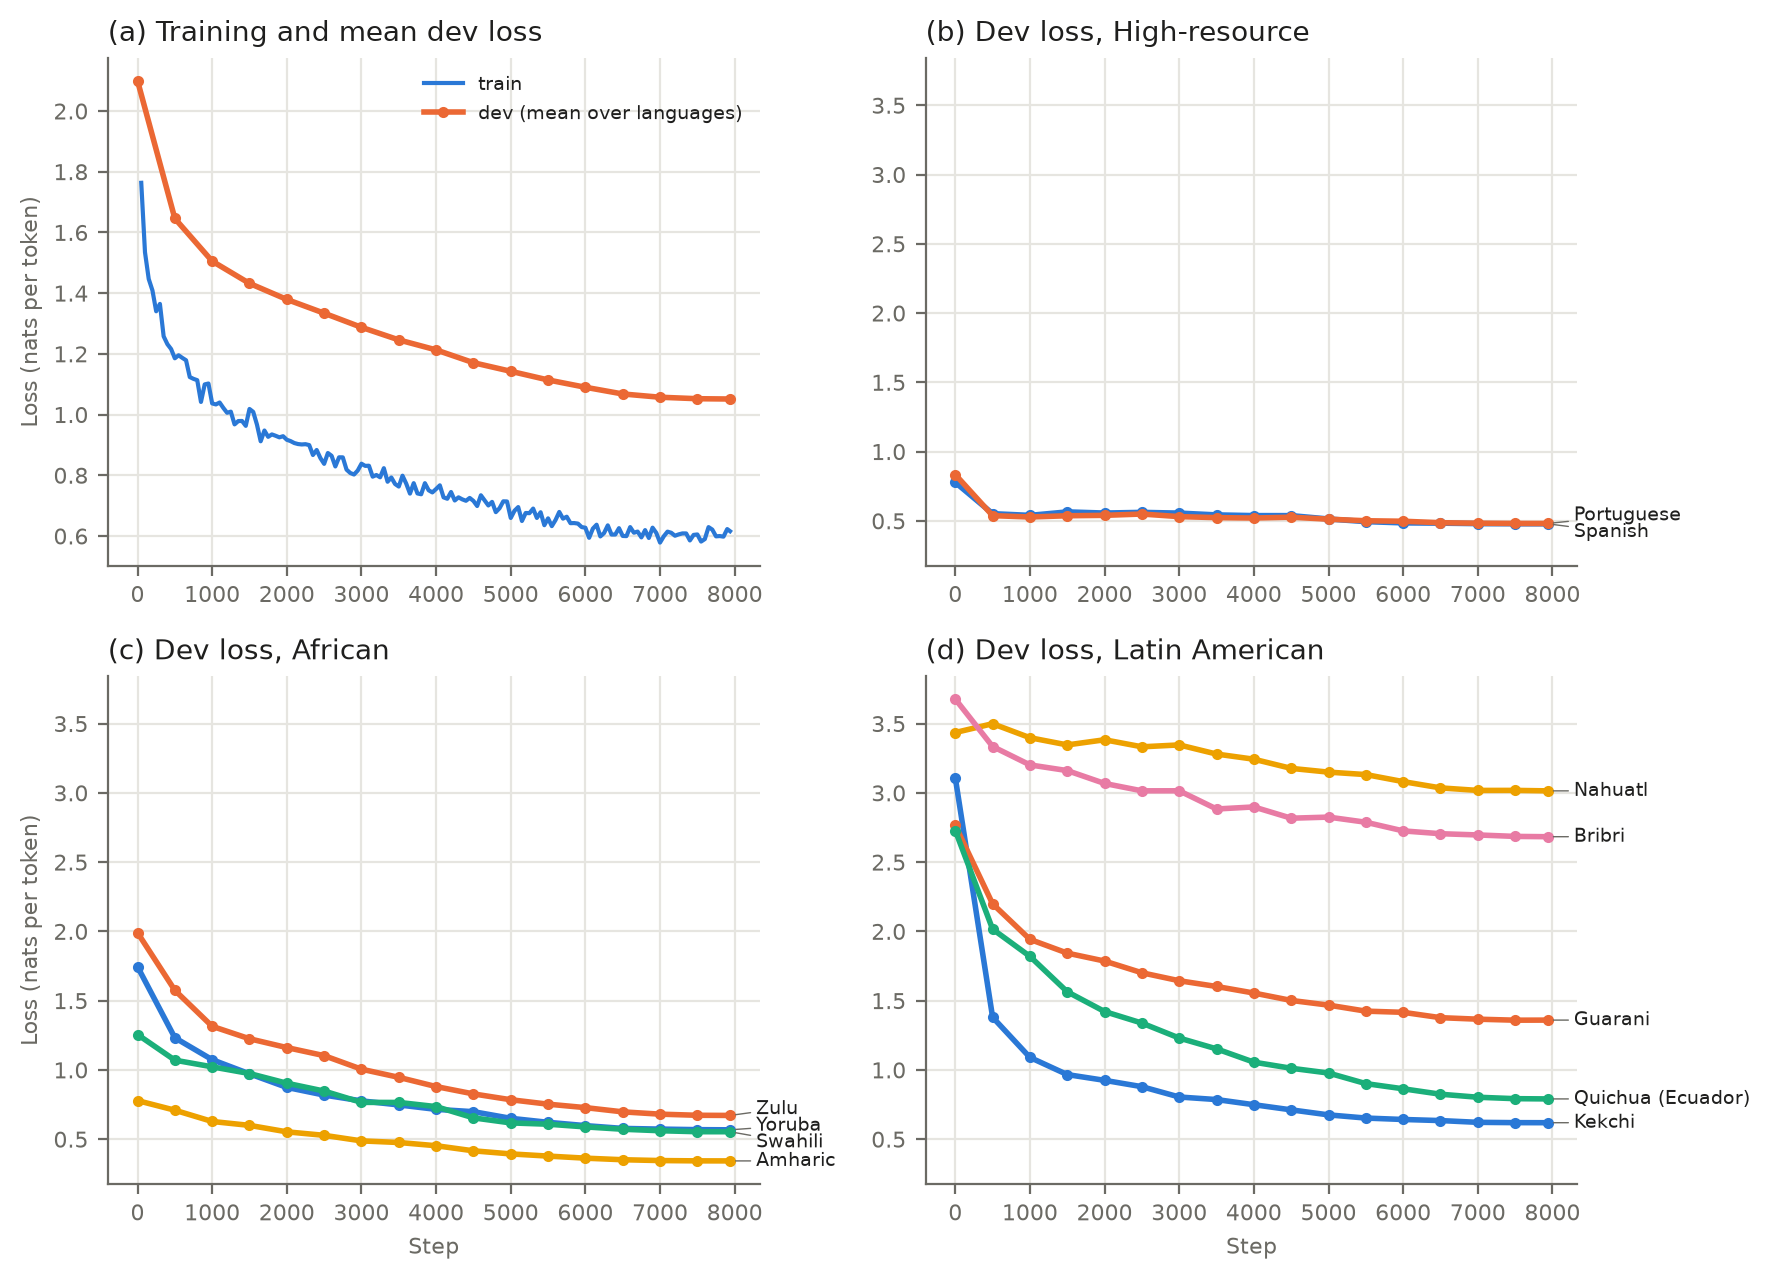
\includegraphics[width=\textwidth]{../../../results/analysis/figures/finetune_loss.png}
\caption{Fine-tuning loss of Llama 3.1 8B. (a) Training loss and dev loss averaged over languages. (b)–(d) Dev loss per language, by group, on the same scale. Losses are per token, so levels are not comparable across languages, only trends within one.}
\end{figure}

\begin{figure}[htbp]
\centering
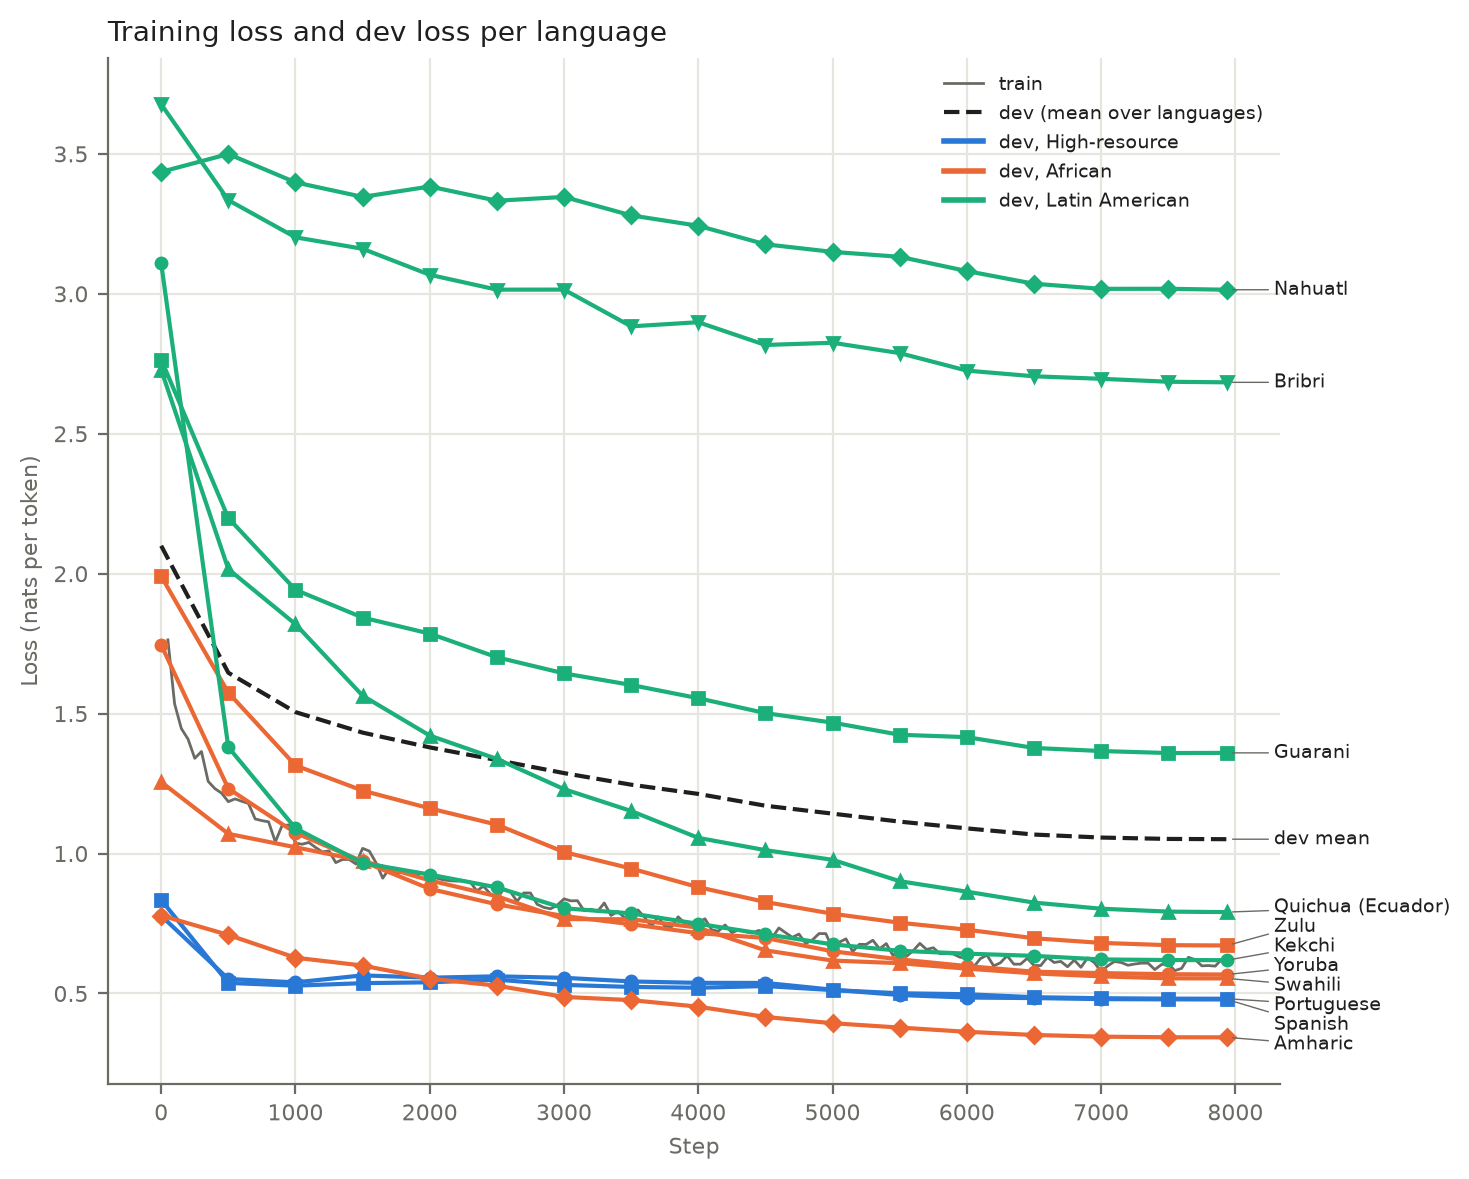
\includegraphics[width=\textwidth]{../../../results/analysis/figures/finetune_loss_overlap.png}
\caption{The curves of Figure 1 in one panel. Colour is the language group and the marker the language.}
\end{figure}

\paragraph{Evaluation.} Every model translates every test set in both directions, English$\rightarrow$X and X$\rightarrow$English, and each direction is scored separately. The models are base models, so we prompt them without a chat template. The prompt has three example pairs from the dev split followed by the source sentence, \texttt{\textless{}eng\textgreater{}\ldots{}\textless{}/eng\textgreater{} \textless{}yor\textgreater{}\ldots{}\textless{}/yor\textgreater{}} three times, then \texttt{\textless{}eng\textgreater{}\{source\}\textless{}/eng\textgreater{} \textless{}yor\textgreater{}}. Decoding is greedy. Generation stops at the closing tag, or at twice the expected length of the translation, estimated from the source length and the average target/source token ratio of the dev pairs. All models run in bf16.

\paragraph{Metrics.} For every model, test set and direction we record three groups of metrics. Translation quality: chrF++ (Popović, 2017) and BLEU (Papineni et al., 2002), computed with sacreBLEU (Post, 2018), AfriCOMET (Wang et al., 2024) for French and the four African languages, and the off-target rate measured with GlotLID (Kargaran et al., 2023). For English$\rightarrow$X the off-target rate is the share of outputs identified as English, and for X$\rightarrow$English the share not identified as English. The other two groups need no generation. Reference likelihood: the negative log-likelihood (NLL) the model gives the human reference translation after the prompt, per word and per byte, and its perplexity per token. Sentence likelihood: the perplexity of each test sentence on its own, after only a start-of-text token, for both its English and its X side, with its NLL per word and per byte. We report per-word and per-byte values because tokenizers split low-resource languages into many more tokens, so per-token values cannot be compared across languages.

Tables 4 to 7 summarize how much each language loses with quantization. They show Llama 3.1 8B and its LoRA fine-tune. Qwen 2.5 7B is in the appendix. Languages are grouped by resource level. For each model, the first column is the full-precision score and the next three are the loss of RTN, GPTQ and AWQ, so a larger number means more degradation. Loss cells are shaded by their size. Tables 4 and 6 give the chrF++ drop at 4 and 3 bits, English$\rightarrow$X first and X$\rightarrow$English second. From English the base models translate most low-resource languages poorly, so their English$\rightarrow$X scores start low and have little room to drop. Tables 5 and 7 give the increase in sentence NLL per byte of the X side, which does not depend on generation. GPTQ and AWQ are the mean over the five calibration seeds. Every result is in the appendix.

\begin{table}[htbp]
\centering
\footnotesize
\setlength{\tabcolsep}{3pt}
\caption{chrF++ drop (FP minus quantized), 4-bit.}
\begin{tabular}{lrrrrrrrr}
\toprule
 & \multicolumn{4}{c}{Llama} & \multicolumn{4}{c}{LoRA} \\
\cmidrule(lr){2-5}\cmidrule(lr){6-9}
Language (test set) & FP & RTN & GPTQ & AWQ & FP & RTN & GPTQ & AWQ \\
\midrule
\multicolumn{9}{l}{\textbf{English$\rightarrow$X}} \\ \midrule
\multicolumn{9}{l}{\textit{High-resource}} \\
French (FLORES+) & 64.0 & \cellcolor{loss!15}1.5 & \cellcolor{loss!10}1.0 & \cellcolor{loss!10}1.0 & 63.0 & \cellcolor{loss!8}0.9 & \cellcolor{loss!6}0.7 & \cellcolor{loss!6}0.6 \\
French (church) & 56.9 & \cellcolor{loss!4}0.4 & \cellcolor{loss!7}0.7 & \cellcolor{loss!10}1.0 & 58.6 & \cellcolor{loss!6}0.7 & \cellcolor{loss!6}0.6 & \cellcolor{loss!5}0.5 \\
Spanish (FLORES+) & 51.9 & \cellcolor{loss!8}0.8 & \cellcolor{loss!6}0.6 & \cellcolor{loss!4}0.4 & 51.5 & \cellcolor{loss!2}0.2 & \cellcolor{loss!1}0.1 & \cellcolor{loss!3}0.3 \\
Spanish (church) & 64.1 & \cellcolor{loss!13}1.3 & \cellcolor{loss!8}0.8 & \cellcolor{loss!10}1.0 & 70.7 & \cellcolor{loss!2}0.2 & \cellcolor{loss!2}0.2 & \cellcolor{loss!3}0.3 \\
Portuguese (FLORES+) & 64.3 & \cellcolor{loss!18}1.9 & \cellcolor{loss!9}0.9 & \cellcolor{loss!6}0.6 & 64.3 & \cellcolor{loss!7}0.7 & \cellcolor{loss!8}0.9 & \cellcolor{loss!8}0.8 \\
Portuguese (church) & 62.5 & \cellcolor{loss!11}1.2 & \cellcolor{loss!7}0.7 & \cellcolor{loss!5}0.5 & 70.8 & \cellcolor{loss!4}0.4 & \cellcolor{loss!5}0.5 & \cellcolor{loss!5}0.6 \\
\midrule \multicolumn{9}{l}{\textit{African}} \\
Yoruba (FLORES+) & 13.2 & \cellcolor{loss!15}1.6 & \cellcolor{loss!16}1.7 & \cellcolor{loss!19}2.0 & 25.6 & \cellcolor{loss!9}1.0 & \cellcolor{loss!3}0.4 & \cellcolor{loss!2}0.2 \\
Yoruba (church) & 15.1 & \cellcolor{loss!33}3.5 & \cellcolor{loss!25}2.6 & \cellcolor{loss!25}2.6 & 60.1 & \cellcolor{loss!13}1.4 & \cellcolor{loss!8}0.9 & \cellcolor{loss!9}0.9 \\
Zulu (FLORES+) & 15.1 & \cellcolor{loss!7}0.8 & \cellcolor{loss!16}1.7 & \cellcolor{loss!3}0.3 & 33.9 & \cellcolor{loss!18}1.9 & \cellcolor{loss!14}1.5 & \cellcolor{loss!13}1.3 \\
Zulu (church) & 15.4 & 0.0 & \cellcolor{loss!5}0.5 & -0.5 & 56.5 & \cellcolor{loss!13}1.3 & \cellcolor{loss!8}0.9 & \cellcolor{loss!6}0.6 \\
Swahili (FLORES+) & 37.4 & \cellcolor{loss!56}5.8 & \cellcolor{loss!45}4.8 & \cellcolor{loss!51}5.3 & 47.2 & \cellcolor{loss!13}1.3 & \cellcolor{loss!10}1.0 & \cellcolor{loss!6}0.6 \\
Swahili (church) & 37.0 & \cellcolor{loss!60}6.3 & \cellcolor{loss!30}3.1 & \cellcolor{loss!44}4.6 & 66.7 & \cellcolor{loss!12}1.3 & \cellcolor{loss!11}1.1 & \cellcolor{loss!10}1.1 \\
Amharic (FLORES+) & 6.5 & \cellcolor{loss!26}2.7 & \cellcolor{loss!23}2.4 & \cellcolor{loss!18}1.9 & 19.5 & \cellcolor{loss!20}2.1 & \cellcolor{loss!18}1.9 & \cellcolor{loss!17}1.8 \\
Amharic (church) & 6.3 & \cellcolor{loss!27}2.8 & \cellcolor{loss!20}2.1 & \cellcolor{loss!14}1.4 & 38.5 & \cellcolor{loss!14}1.5 & \cellcolor{loss!16}1.6 & \cellcolor{loss!12}1.2 \\
\midrule \multicolumn{9}{l}{\textit{Latin American}} \\
Kekchi (MayanV) & 7.9 & \cellcolor{loss!21}2.2 & \cellcolor{loss!15}1.6 & \cellcolor{loss!26}2.7 & 18.5 & \cellcolor{loss!6}0.6 & \cellcolor{loss!2}0.2 & \cellcolor{loss!2}0.2 \\
Kekchi (church) & 13.7 & -0.3 & \cellcolor{loss!5}0.5 & -0.3 & 61.6 & \cellcolor{loss!7}0.8 & \cellcolor{loss!4}0.5 & \cellcolor{loss!4}0.4 \\
Guarani (FLORES+) & 14.4 & -1.5 & -1.0 & \cellcolor{loss!4}0.4 & 33.5 & \cellcolor{loss!7}0.8 & \cellcolor{loss!7}0.8 & \cellcolor{loss!6}0.7 \\
Guarani (church) & 11.3 & -1.5 & -0.2 & -0.5 & 51.9 & \cellcolor{loss!8}0.8 & \cellcolor{loss!5}0.5 & \cellcolor{loss!4}0.4 \\
Quichua (Ecuador) (church) & 13.1 & -2.1 & \cellcolor{loss!4}0.4 & -1.7 & 57.4 & \cellcolor{loss!17}1.8 & \cellcolor{loss!8}0.8 & \cellcolor{loss!8}0.8 \\
Nahuatl (AmericasNLP) & 13.2 & -0.2 & \cellcolor{loss!7}0.7 & \cellcolor{loss!7}0.7 & 13.4 & \cellcolor{loss!14}1.4 & \cellcolor{loss!5}0.5 & \cellcolor{loss!5}0.5 \\
Bribri (AmericasNLP) & 7.7 & -0.3 & -0.6 & \cellcolor{loss!4}0.4 & 11.7 & \cellcolor{loss!5}0.5 & \cellcolor{loss!3}0.3 & \cellcolor{loss!7}0.7 \\
\midrule \multicolumn{9}{l}{\textbf{X$\rightarrow$English}} \\ \midrule
\multicolumn{9}{l}{\textit{High-resource}} \\
French (FLORES+) & 64.4 & \cellcolor{loss!7}1.0 & \cellcolor{loss!2}0.3 & \cellcolor{loss!1}0.2 & 65.4 & \cellcolor{loss!3}0.5 & \cellcolor{loss!2}0.3 & \cellcolor{loss!3}0.4 \\
French (church) & 61.6 & \cellcolor{loss!8}1.1 & \cellcolor{loss!6}0.9 & \cellcolor{loss!3}0.5 & 69.1 & \cellcolor{loss!10}1.5 & \cellcolor{loss!4}0.6 & \cellcolor{loss!5}0.7 \\
Spanish (FLORES+) & 57.2 & \cellcolor{loss!4}0.6 & \cellcolor{loss!1}0.2 & \cellcolor{loss!0}0.1 & 58.1 & \cellcolor{loss!4}0.6 & \cellcolor{loss!2}0.3 & \cellcolor{loss!2}0.4 \\
Spanish (church) & 70.0 & \cellcolor{loss!7}1.0 & \cellcolor{loss!5}0.8 & \cellcolor{loss!8}1.2 & 77.0 & \cellcolor{loss!4}0.6 & \cellcolor{loss!2}0.4 & \cellcolor{loss!2}0.3 \\
Portuguese (FLORES+) & 68.8 & \cellcolor{loss!8}1.2 & \cellcolor{loss!4}0.6 & \cellcolor{loss!3}0.4 & 68.7 & \cellcolor{loss!2}0.3 & \cellcolor{loss!1}0.2 & \cellcolor{loss!4}0.6 \\
Portuguese (church) & 69.6 & \cellcolor{loss!12}1.8 & \cellcolor{loss!9}1.3 & \cellcolor{loss!8}1.2 & 76.1 & \cellcolor{loss!3}0.5 & \cellcolor{loss!3}0.4 & \cellcolor{loss!2}0.3 \\
\midrule \multicolumn{9}{l}{\textit{African}} \\
Yoruba (FLORES+) & 28.3 & \cellcolor{loss!25}3.7 & \cellcolor{loss!10}1.4 & \cellcolor{loss!8}1.2 & 33.3 & \cellcolor{loss!12}1.7 & \cellcolor{loss!7}1.0 & \cellcolor{loss!7}1.0 \\
Yoruba (church) & 29.9 & \cellcolor{loss!46}6.8 & \cellcolor{loss!25}3.7 & \cellcolor{loss!23}3.3 & 70.1 & \cellcolor{loss!18}2.6 & \cellcolor{loss!7}1.0 & \cellcolor{loss!7}1.0 \\
Zulu (FLORES+) & 31.1 & \cellcolor{loss!33}4.9 & \cellcolor{loss!11}1.6 & \cellcolor{loss!9}1.3 & 41.6 & \cellcolor{loss!13}1.9 & \cellcolor{loss!6}0.9 & \cellcolor{loss!9}1.3 \\
Zulu (church) & 34.4 & \cellcolor{loss!36}5.3 & \cellcolor{loss!15}2.2 & \cellcolor{loss!13}2.0 & 68.1 & \cellcolor{loss!15}2.1 & \cellcolor{loss!11}1.6 & \cellcolor{loss!9}1.3 \\
Swahili (FLORES+) & 53.6 & \cellcolor{loss!60}8.8 & \cellcolor{loss!21}3.1 & \cellcolor{loss!16}2.4 & 54.2 & \cellcolor{loss!19}2.8 & \cellcolor{loss!11}1.6 & \cellcolor{loss!12}1.7 \\
Swahili (church) & 60.3 & \cellcolor{loss!53}7.7 & \cellcolor{loss!23}3.3 & \cellcolor{loss!23}3.4 & 75.2 & \cellcolor{loss!12}1.7 & \cellcolor{loss!4}0.6 & \cellcolor{loss!3}0.5 \\
Amharic (FLORES+) & 28.7 & \cellcolor{loss!45}6.5 & \cellcolor{loss!30}4.3 & \cellcolor{loss!19}2.8 & 36.1 & \cellcolor{loss!13}2.0 & \cellcolor{loss!6}0.9 & \cellcolor{loss!7}1.0 \\
Amharic (church) & 27.4 & \cellcolor{loss!58}8.4 & \cellcolor{loss!38}5.5 & \cellcolor{loss!25}3.6 & 59.1 & \cellcolor{loss!19}2.8 & \cellcolor{loss!10}1.4 & \cellcolor{loss!11}1.6 \\
\midrule \multicolumn{9}{l}{\textit{Latin American}} \\
Kekchi (MayanV) & 9.5 & -0.2 & -0.8 & -0.5 & 25.8 & \cellcolor{loss!9}1.4 & \cellcolor{loss!3}0.5 & \cellcolor{loss!3}0.4 \\
Kekchi (church) & 22.6 & \cellcolor{loss!9}1.3 & \cellcolor{loss!5}0.7 & \cellcolor{loss!4}0.6 & 60.8 & \cellcolor{loss!10}1.4 & \cellcolor{loss!3}0.5 & \cellcolor{loss!6}0.8 \\
Guarani (FLORES+) & 30.5 & \cellcolor{loss!21}3.1 & \cellcolor{loss!5}0.8 & \cellcolor{loss!6}0.9 & 41.7 & \cellcolor{loss!10}1.4 & \cellcolor{loss!4}0.5 & \cellcolor{loss!5}0.8 \\
Guarani (church) & 30.6 & \cellcolor{loss!30}4.4 & \cellcolor{loss!6}0.9 & \cellcolor{loss!21}3.1 & 64.8 & \cellcolor{loss!17}2.4 & \cellcolor{loss!7}1.0 & \cellcolor{loss!8}1.2 \\
Quichua (Ecuador) (church) & 23.1 & -0.2 & -0.6 & -0.3 & 56.5 & \cellcolor{loss!30}4.3 & \cellcolor{loss!14}2.1 & \cellcolor{loss!16}2.3 \\
Nahuatl (AmericasNLP) & 18.0 & \cellcolor{loss!6}0.9 & \cellcolor{loss!0}0.1 & \cellcolor{loss!4}0.6 & 20.1 & \cellcolor{loss!8}1.1 & \cellcolor{loss!2}0.3 & \cellcolor{loss!3}0.4 \\
Bribri (AmericasNLP) & 17.3 & -0.2 & \cellcolor{loss!0}0.0 & \cellcolor{loss!0}0.0 & 20.1 & \cellcolor{loss!5}0.8 & \cellcolor{loss!1}0.2 & \cellcolor{loss!2}0.3 \\
\bottomrule
\end{tabular}
\end{table}

\begin{table}[htbp]
\centering
\footnotesize
\setlength{\tabcolsep}{3pt}
\caption{Increase in sentence NLL per byte, X side (quantized minus FP), 4-bit.}
\begin{tabular}{lrrrrrrrr}
\toprule
 & \multicolumn{4}{c}{Llama} & \multicolumn{4}{c}{LoRA} \\
\cmidrule(lr){2-5}\cmidrule(lr){6-9}
Language (test set) & FP & RTN & GPTQ & AWQ & FP & RTN & GPTQ & AWQ \\
\midrule
\multicolumn{9}{l}{\textit{High-resource}} \\
French (FLORES+) & 0.63 & \cellcolor{loss!5}0.020 & \cellcolor{loss!2}0.010 & \cellcolor{loss!2}0.010 & 0.70 & \cellcolor{loss!9}0.040 & \cellcolor{loss!5}0.020 & \cellcolor{loss!5}0.020 \\
French (church) & 0.81 & \cellcolor{loss!7}0.030 & \cellcolor{loss!2}0.010 & \cellcolor{loss!2}0.010 & 0.84 & \cellcolor{loss!12}0.050 & \cellcolor{loss!6}0.028 & \cellcolor{loss!5}0.020 \\
Spanish (FLORES+) & 0.69 & \cellcolor{loss!7}0.030 & \cellcolor{loss!5}0.020 & \cellcolor{loss!4}0.018 & 0.76 & \cellcolor{loss!7}0.030 & \cellcolor{loss!4}0.016 & \cellcolor{loss!2}0.010 \\
Spanish (church) & 0.84 & \cellcolor{loss!7}0.030 & \cellcolor{loss!4}0.018 & \cellcolor{loss!2}0.010 & 0.82 & \cellcolor{loss!7}0.030 & \cellcolor{loss!4}0.016 & \cellcolor{loss!3}0.014 \\
Portuguese (FLORES+) & 0.73 & \cellcolor{loss!7}0.030 & \cellcolor{loss!5}0.020 & \cellcolor{loss!2}0.010 & 0.80 & \cellcolor{loss!9}0.040 & \cellcolor{loss!7}0.030 & \cellcolor{loss!7}0.030 \\
Portuguese (church) & 0.90 & \cellcolor{loss!7}0.030 & \cellcolor{loss!6}0.024 & \cellcolor{loss!5}0.020 & 0.90 & \cellcolor{loss!7}0.030 & \cellcolor{loss!6}0.026 & \cellcolor{loss!5}0.020 \\
\midrule \multicolumn{9}{l}{\textit{African}} \\
Yoruba (FLORES+) & 1.40 & \cellcolor{loss!30}0.130 & \cellcolor{loss!21}0.092 & \cellcolor{loss!14}0.060 & 1.61 & \cellcolor{loss!16}0.070 & \cellcolor{loss!12}0.054 & \cellcolor{loss!10}0.042 \\
Yoruba (church) & 1.36 & \cellcolor{loss!32}0.140 & \cellcolor{loss!22}0.094 & \cellcolor{loss!15}0.064 & 1.25 & \cellcolor{loss!23}0.100 & \cellcolor{loss!18}0.080 & \cellcolor{loss!15}0.064 \\
Zulu (FLORES+) & 1.45 & \cellcolor{loss!32}0.140 & \cellcolor{loss!23}0.098 & \cellcolor{loss!19}0.084 & 1.77 & \cellcolor{loss!21}0.090 & \cellcolor{loss!19}0.082 & \cellcolor{loss!13}0.058 \\
Zulu (church) & 1.60 & \cellcolor{loss!25}0.110 & \cellcolor{loss!18}0.080 & \cellcolor{loss!15}0.066 & 1.65 & \cellcolor{loss!18}0.080 & \cellcolor{loss!19}0.084 & \cellcolor{loss!14}0.060 \\
Swahili (FLORES+) & 1.16 & \cellcolor{loss!28}0.120 & \cellcolor{loss!17}0.072 & \cellcolor{loss!14}0.060 & 1.43 & \cellcolor{loss!25}0.110 & \cellcolor{loss!21}0.092 & \cellcolor{loss!13}0.058 \\
Swahili (church) & 1.32 & \cellcolor{loss!23}0.100 & \cellcolor{loss!16}0.070 & \cellcolor{loss!14}0.062 & 1.41 & \cellcolor{loss!25}0.110 & \cellcolor{loss!24}0.104 & \cellcolor{loss!14}0.060 \\
Amharic (FLORES+) & 0.85 & \cellcolor{loss!60}0.260 & \cellcolor{loss!42}0.182 & \cellcolor{loss!27}0.118 & 1.12 & \cellcolor{loss!14}0.060 & \cellcolor{loss!15}0.066 & \cellcolor{loss!12}0.052 \\
Amharic (church) & 0.89 & \cellcolor{loss!60}0.260 & \cellcolor{loss!40}0.172 & \cellcolor{loss!27}0.116 & 0.91 & \cellcolor{loss!18}0.080 & \cellcolor{loss!17}0.074 & \cellcolor{loss!10}0.042 \\
\midrule \multicolumn{9}{l}{\textit{Latin American}} \\
Kekchi (MayanV) & 3.21 & \cellcolor{loss!18}0.080 & \cellcolor{loss!10}0.042 & \cellcolor{loss!14}0.060 & 2.44 & \cellcolor{loss!23}0.100 & \cellcolor{loss!14}0.062 & \cellcolor{loss!14}0.062 \\
Kekchi (church) & 2.47 & \cellcolor{loss!12}0.050 & \cellcolor{loss!8}0.034 & \cellcolor{loss!7}0.032 & 1.14 & \cellcolor{loss!14}0.060 & \cellcolor{loss!12}0.052 & \cellcolor{loss!8}0.034 \\
Guarani (FLORES+) & 1.74 & \cellcolor{loss!32}0.140 & \cellcolor{loss!23}0.098 & \cellcolor{loss!21}0.092 & 1.56 & \cellcolor{loss!12}0.050 & \cellcolor{loss!9}0.040 & \cellcolor{loss!12}0.050 \\
Guarani (church) & 1.91 & \cellcolor{loss!28}0.120 & \cellcolor{loss!21}0.092 & \cellcolor{loss!20}0.088 & 1.47 & \cellcolor{loss!14}0.060 & \cellcolor{loss!12}0.054 & \cellcolor{loss!12}0.054 \\
Quichua (Ecuador) (church) & 2.05 & \cellcolor{loss!12}0.050 & \cellcolor{loss!7}0.030 & \cellcolor{loss!7}0.032 & 1.96 & 0.000 & \cellcolor{loss!4}0.016 & \cellcolor{loss!0}0.002 \\
Nahuatl (AmericasNLP) & 2.50 & \cellcolor{loss!7}0.030 & \cellcolor{loss!8}0.034 & \cellcolor{loss!13}0.056 & 2.42 & \cellcolor{loss!25}0.110 & \cellcolor{loss!12}0.054 & \cellcolor{loss!12}0.054 \\
Bribri (AmericasNLP) & 3.02 & \cellcolor{loss!14}0.060 & \cellcolor{loss!3}0.012 & \cellcolor{loss!9}0.038 & 2.32 & \cellcolor{loss!21}0.090 & \cellcolor{loss!7}0.030 & \cellcolor{loss!11}0.046 \\
\bottomrule
\end{tabular}
\end{table}

\begin{table}[htbp]
\centering
\footnotesize
\setlength{\tabcolsep}{3pt}
\caption{chrF++ drop (FP minus quantized), 3-bit.}
\begin{tabular}{lrrrrrrrr}
\toprule
 & \multicolumn{4}{c}{Llama} & \multicolumn{4}{c}{LoRA} \\
\cmidrule(lr){2-5}\cmidrule(lr){6-9}
Language (test set) & FP & RTN & GPTQ & AWQ & FP & RTN & GPTQ & AWQ \\
\midrule
\multicolumn{9}{l}{\textbf{English$\rightarrow$X}} \\ \midrule
\multicolumn{9}{l}{\textit{High-resource}} \\
French (FLORES+) & 64.0 & \cellcolor{loss!17}9.5 & \cellcolor{loss!11}5.8 & \cellcolor{loss!11}5.9 & 63.0 & \cellcolor{loss!16}8.9 & \cellcolor{loss!7}3.9 & \cellcolor{loss!7}3.9 \\
French (church) & 56.9 & \cellcolor{loss!11}6.2 & \cellcolor{loss!8}4.1 & \cellcolor{loss!7}4.0 & 58.6 & \cellcolor{loss!16}9.0 & \cellcolor{loss!5}2.9 & \cellcolor{loss!6}3.1 \\
Spanish (FLORES+) & 51.9 & \cellcolor{loss!9}5.1 & \cellcolor{loss!5}2.7 & \cellcolor{loss!6}3.2 & 51.5 & \cellcolor{loss!9}4.7 & \cellcolor{loss!3}1.8 & \cellcolor{loss!3}1.9 \\
Spanish (church) & 64.1 & \cellcolor{loss!16}8.7 & \cellcolor{loss!9}4.8 & \cellcolor{loss!8}4.5 & 70.7 & \cellcolor{loss!10}5.7 & \cellcolor{loss!4}2.1 & \cellcolor{loss!4}2.0 \\
Portuguese (FLORES+) & 64.3 & \cellcolor{loss!18}9.6 & \cellcolor{loss!9}5.1 & \cellcolor{loss!10}5.2 & 64.3 & \cellcolor{loss!13}7.2 & \cellcolor{loss!7}3.7 & \cellcolor{loss!6}3.3 \\
Portuguese (church) & 62.5 & \cellcolor{loss!14}7.8 & \cellcolor{loss!9}5.1 & \cellcolor{loss!9}4.9 & 70.8 & \cellcolor{loss!11}6.2 & \cellcolor{loss!7}3.6 & \cellcolor{loss!5}2.9 \\
\midrule \multicolumn{9}{l}{\textit{African}} \\
Yoruba (FLORES+) & 13.2 & \cellcolor{loss!4}2.4 & \cellcolor{loss!14}7.9 & \cellcolor{loss!10}5.6 & 25.6 & \cellcolor{loss!27}14.6 & \cellcolor{loss!6}3.4 & \cellcolor{loss!5}2.8 \\
Yoruba (church) & 15.1 & \cellcolor{loss!15}8.3 & \cellcolor{loss!16}8.9 & \cellcolor{loss!11}6.0 & 60.1 & \cellcolor{loss!56}30.7 & \cellcolor{loss!15}8.3 & \cellcolor{loss!10}5.6 \\
Zulu (FLORES+) & 15.1 & \cellcolor{loss!5}2.7 & \cellcolor{loss!10}5.2 & \cellcolor{loss!8}4.6 & 33.9 & \cellcolor{loss!32}17.7 & \cellcolor{loss!12}6.5 & \cellcolor{loss!11}5.9 \\
Zulu (church) & 15.4 & \cellcolor{loss!13}7.4 & \cellcolor{loss!8}4.6 & \cellcolor{loss!6}3.3 & 56.5 & \cellcolor{loss!36}19.8 & \cellcolor{loss!12}6.5 & \cellcolor{loss!9}5.2 \\
Swahili (FLORES+) & 37.4 & \cellcolor{loss!50}27.6 & \cellcolor{loss!35}19.0 & \cellcolor{loss!34}18.9 & 47.2 & \cellcolor{loss!45}24.7 & \cellcolor{loss!13}7.3 & \cellcolor{loss!12}6.3 \\
Swahili (church) & 37.0 & \cellcolor{loss!46}25.1 & \cellcolor{loss!32}17.4 & \cellcolor{loss!30}16.6 & 66.7 & \cellcolor{loss!45}24.8 & \cellcolor{loss!12}6.4 & \cellcolor{loss!10}5.5 \\
Amharic (FLORES+) & 6.5 & \cellcolor{loss!11}6.1 & \cellcolor{loss!9}5.2 & \cellcolor{loss!9}5.0 & 19.5 & \cellcolor{loss!32}17.4 & \cellcolor{loss!22}12.0 & \cellcolor{loss!17}9.4 \\
Amharic (church) & 6.3 & \cellcolor{loss!10}5.7 & \cellcolor{loss!9}4.9 & \cellcolor{loss!8}4.5 & 38.5 & \cellcolor{loss!60}32.8 & \cellcolor{loss!36}19.9 & \cellcolor{loss!20}11.0 \\
\midrule \multicolumn{9}{l}{\textit{Latin American}} \\
Kekchi (MayanV) & 7.9 & \cellcolor{loss!2}0.8 & \cellcolor{loss!5}2.7 & \cellcolor{loss!8}4.2 & 18.5 & \cellcolor{loss!8}4.3 & \cellcolor{loss!3}1.6 & \cellcolor{loss!2}1.3 \\
Kekchi (church) & 13.7 & \cellcolor{loss!4}2.3 & \cellcolor{loss!5}2.7 & \cellcolor{loss!3}1.6 & 61.6 & \cellcolor{loss!23}12.5 & \cellcolor{loss!6}3.0 & \cellcolor{loss!6}3.4 \\
Guarani (FLORES+) & 14.4 & \cellcolor{loss!6}3.5 & \cellcolor{loss!6}3.4 & \cellcolor{loss!12}6.3 & 33.5 & \cellcolor{loss!14}7.9 & \cellcolor{loss!5}3.0 & \cellcolor{loss!6}3.4 \\
Guarani (church) & 11.3 & \cellcolor{loss!1}0.8 & \cellcolor{loss!5}2.7 & \cellcolor{loss!3}1.6 & 51.9 & \cellcolor{loss!25}13.4 & \cellcolor{loss!7}4.0 & \cellcolor{loss!7}4.0 \\
Quichua (Ecuador) (church) & 13.1 & \cellcolor{loss!5}2.5 & -0.8 & \cellcolor{loss!0}0.1 & 57.4 & \cellcolor{loss!52}28.3 & \cellcolor{loss!15}7.9 & \cellcolor{loss!16}8.9 \\
Nahuatl (AmericasNLP) & 13.2 & \cellcolor{loss!8}4.5 & \cellcolor{loss!6}3.5 & \cellcolor{loss!5}3.0 & 13.4 & \cellcolor{loss!5}3.0 & \cellcolor{loss!4}2.4 & \cellcolor{loss!5}2.6 \\
Bribri (AmericasNLP) & 7.7 & -0.8 & \cellcolor{loss!1}0.3 & \cellcolor{loss!4}2.0 & 11.7 & \cellcolor{loss!5}2.6 & \cellcolor{loss!3}1.8 & \cellcolor{loss!5}2.5 \\
\midrule \multicolumn{9}{l}{\textbf{X$\rightarrow$English}} \\ \midrule
\multicolumn{9}{l}{\textit{High-resource}} \\
French (FLORES+) & 64.4 & \cellcolor{loss!11}8.1 & \cellcolor{loss!3}1.9 & \cellcolor{loss!2}1.6 & 65.4 & \cellcolor{loss!11}8.0 & \cellcolor{loss!3}1.8 & \cellcolor{loss!3}2.4 \\
French (church) & 61.6 & \cellcolor{loss!9}6.6 & \cellcolor{loss!5}3.8 & \cellcolor{loss!3}2.4 & 69.1 & \cellcolor{loss!14}10.0 & \cellcolor{loss!4}2.8 & \cellcolor{loss!4}3.2 \\
Spanish (FLORES+) & 57.2 & \cellcolor{loss!9}6.7 & \cellcolor{loss!2}1.7 & \cellcolor{loss!3}1.9 & 58.1 & \cellcolor{loss!10}6.9 & \cellcolor{loss!3}1.8 & \cellcolor{loss!3}2.2 \\
Spanish (church) & 70.0 & \cellcolor{loss!12}8.4 & \cellcolor{loss!6}4.1 & \cellcolor{loss!5}3.4 & 77.0 & \cellcolor{loss!9}6.8 & \cellcolor{loss!3}2.1 & \cellcolor{loss!3}2.5 \\
Portuguese (FLORES+) & 68.8 & \cellcolor{loss!19}13.8 & \cellcolor{loss!4}2.6 & \cellcolor{loss!3}2.2 & 68.7 & \cellcolor{loss!13}9.0 & \cellcolor{loss!3}2.0 & \cellcolor{loss!3}2.3 \\
Portuguese (church) & 69.6 & \cellcolor{loss!14}9.9 & \cellcolor{loss!6}4.3 & \cellcolor{loss!5}3.7 & 76.1 & \cellcolor{loss!11}8.2 & \cellcolor{loss!3}2.4 & \cellcolor{loss!3}2.3 \\
\midrule \multicolumn{9}{l}{\textit{African}} \\
Yoruba (FLORES+) & 28.3 & \cellcolor{loss!14}9.9 & \cellcolor{loss!10}7.4 & \cellcolor{loss!7}5.1 & 33.3 & \cellcolor{loss!20}14.5 & \cellcolor{loss!6}4.6 & \cellcolor{loss!6}4.5 \\
Yoruba (church) & 29.9 & \cellcolor{loss!22}15.7 & \cellcolor{loss!15}11.1 & \cellcolor{loss!12}9.0 & 70.1 & \cellcolor{loss!60}43.3 & \cellcolor{loss!14}10.0 & \cellcolor{loss!11}7.6 \\
Zulu (FLORES+) & 31.1 & \cellcolor{loss!18}12.8 & \cellcolor{loss!13}9.1 & \cellcolor{loss!9}6.2 & 41.6 & \cellcolor{loss!27}19.8 & \cellcolor{loss!8}5.6 & \cellcolor{loss!8}6.1 \\
Zulu (church) & 34.4 & \cellcolor{loss!27}19.6 & \cellcolor{loss!19}13.5 & \cellcolor{loss!13}9.4 & 68.1 & \cellcolor{loss!51}36.6 & \cellcolor{loss!13}9.4 & \cellcolor{loss!11}8.1 \\
Swahili (FLORES+) & 53.6 & \cellcolor{loss!48}34.5 & \cellcolor{loss!26}18.6 & \cellcolor{loss!22}16.0 & 54.2 & \cellcolor{loss!42}30.6 & \cellcolor{loss!11}8.3 & \cellcolor{loss!12}8.9 \\
Swahili (church) & 60.3 & \cellcolor{loss!58}41.8 & \cellcolor{loss!31}22.5 & \cellcolor{loss!25}18.3 & 75.2 & \cellcolor{loss!57}41.1 & \cellcolor{loss!9}6.5 & \cellcolor{loss!8}5.6 \\
Amharic (FLORES+) & 28.7 & \cellcolor{loss!19}14.0 & \cellcolor{loss!18}13.2 & \cellcolor{loss!16}11.4 & 36.1 & \cellcolor{loss!29}20.7 & \cellcolor{loss!15}10.7 & \cellcolor{loss!9}6.8 \\
Amharic (church) & 27.4 & \cellcolor{loss!36}26.0 & \cellcolor{loss!24}17.5 & \cellcolor{loss!19}13.4 & 59.1 & \cellcolor{loss!58}42.2 & \cellcolor{loss!30}21.4 & \cellcolor{loss!13}9.6 \\
\midrule \multicolumn{9}{l}{\textit{Latin American}} \\
Kekchi (MayanV) & 9.5 & \cellcolor{loss!5}3.4 & \cellcolor{loss!1}0.4 & -0.0 & 25.8 & \cellcolor{loss!18}13.2 & \cellcolor{loss!8}6.1 & \cellcolor{loss!4}2.7 \\
Kekchi (church) & 22.6 & \cellcolor{loss!13}9.5 & \cellcolor{loss!7}5.2 & \cellcolor{loss!4}2.7 & 60.8 & \cellcolor{loss!31}22.1 & \cellcolor{loss!6}4.0 & \cellcolor{loss!5}3.9 \\
Guarani (FLORES+) & 30.5 & \cellcolor{loss!16}11.4 & \cellcolor{loss!7}5.2 & \cellcolor{loss!6}4.1 & 41.7 & \cellcolor{loss!19}13.5 & \cellcolor{loss!5}3.6 & \cellcolor{loss!5}3.8 \\
Guarani (church) & 30.6 & \cellcolor{loss!19}13.7 & \cellcolor{loss!12}8.4 & \cellcolor{loss!7}4.9 & 64.8 & \cellcolor{loss!37}26.4 & \cellcolor{loss!9}6.2 & \cellcolor{loss!8}6.1 \\
Quichua (Ecuador) (church) & 23.1 & \cellcolor{loss!2}1.8 & \cellcolor{loss!1}1.1 & \cellcolor{loss!1}0.7 & 56.5 & \cellcolor{loss!47}34.1 & \cellcolor{loss!15}10.9 & \cellcolor{loss!15}10.6 \\
Nahuatl (AmericasNLP) & 18.0 & \cellcolor{loss!6}4.7 & \cellcolor{loss!4}2.9 & \cellcolor{loss!2}1.1 & 20.1 & \cellcolor{loss!10}6.9 & \cellcolor{loss!3}2.0 & \cellcolor{loss!4}2.6 \\
Bribri (AmericasNLP) & 17.3 & \cellcolor{loss!6}4.4 & \cellcolor{loss!2}1.1 & \cellcolor{loss!1}0.7 & 20.1 & \cellcolor{loss!7}5.2 & \cellcolor{loss!2}1.8 & \cellcolor{loss!2}1.6 \\
\bottomrule
\end{tabular}
\end{table}

\begin{table}[htbp]
\centering
\footnotesize
\setlength{\tabcolsep}{3pt}
\caption{Increase in sentence NLL per byte, X side (quantized minus FP), 3-bit.}
\begin{tabular}{lrrrrrrrr}
\toprule
 & \multicolumn{4}{c}{Llama} & \multicolumn{4}{c}{LoRA} \\
\cmidrule(lr){2-5}\cmidrule(lr){6-9}
Language (test set) & FP & RTN & GPTQ & AWQ & FP & RTN & GPTQ & AWQ \\
\midrule
\multicolumn{9}{l}{\textit{High-resource}} \\
French (FLORES+) & 0.63 & \cellcolor{loss!11}0.200 & \cellcolor{loss!5}0.096 & \cellcolor{loss!4}0.068 & 0.70 & \cellcolor{loss!20}0.370 & \cellcolor{loss!8}0.150 & \cellcolor{loss!6}0.110 \\
French (church) & 0.81 & \cellcolor{loss!13}0.240 & \cellcolor{loss!6}0.116 & \cellcolor{loss!4}0.080 & 0.84 & \cellcolor{loss!22}0.410 & \cellcolor{loss!9}0.156 & \cellcolor{loss!6}0.116 \\
Spanish (FLORES+) & 0.69 & \cellcolor{loss!11}0.200 & \cellcolor{loss!6}0.104 & \cellcolor{loss!4}0.070 & 0.76 & \cellcolor{loss!17}0.320 & \cellcolor{loss!7}0.132 & \cellcolor{loss!5}0.092 \\
Spanish (church) & 0.84 & \cellcolor{loss!13}0.240 & \cellcolor{loss!7}0.132 & \cellcolor{loss!4}0.080 & 0.82 & \cellcolor{loss!17}0.320 & \cellcolor{loss!7}0.122 & \cellcolor{loss!5}0.086 \\
Portuguese (FLORES+) & 0.73 & \cellcolor{loss!13}0.240 & \cellcolor{loss!7}0.126 & \cellcolor{loss!4}0.078 & 0.80 & \cellcolor{loss!21}0.380 & \cellcolor{loss!9}0.174 & \cellcolor{loss!7}0.122 \\
Portuguese (church) & 0.90 & \cellcolor{loss!15}0.270 & \cellcolor{loss!9}0.164 & \cellcolor{loss!5}0.090 & 0.90 & \cellcolor{loss!20}0.370 & \cellcolor{loss!9}0.162 & \cellcolor{loss!6}0.108 \\
\midrule \multicolumn{9}{l}{\textit{African}} \\
Yoruba (FLORES+) & 1.40 & \cellcolor{loss!33}0.610 & \cellcolor{loss!26}0.472 & \cellcolor{loss!17}0.312 & 1.61 & \cellcolor{loss!30}0.550 & \cellcolor{loss!14}0.258 & \cellcolor{loss!9}0.166 \\
Yoruba (church) & 1.36 & \cellcolor{loss!37}0.670 & \cellcolor{loss!28}0.514 & \cellcolor{loss!18}0.326 & 1.25 & \cellcolor{loss!38}0.700 & \cellcolor{loss!21}0.378 & \cellcolor{loss!13}0.236 \\
Zulu (FLORES+) & 1.45 & \cellcolor{loss!37}0.680 & \cellcolor{loss!27}0.502 & \cellcolor{loss!20}0.358 & 1.77 & \cellcolor{loss!26}0.470 & \cellcolor{loss!16}0.292 & \cellcolor{loss!11}0.200 \\
Zulu (church) & 1.60 & \cellcolor{loss!34}0.630 & \cellcolor{loss!25}0.460 & \cellcolor{loss!17}0.310 & 1.65 & \cellcolor{loss!31}0.560 & \cellcolor{loss!18}0.326 & \cellcolor{loss!10}0.192 \\
Swahili (FLORES+) & 1.16 & \cellcolor{loss!40}0.740 & \cellcolor{loss!26}0.476 & \cellcolor{loss!18}0.338 & 1.43 & \cellcolor{loss!44}0.810 & \cellcolor{loss!17}0.304 & \cellcolor{loss!13}0.242 \\
Swahili (church) & 1.32 & \cellcolor{loss!39}0.710 & \cellcolor{loss!26}0.470 & \cellcolor{loss!19}0.348 & 1.41 & \cellcolor{loss!47}0.870 & \cellcolor{loss!17}0.314 & \cellcolor{loss!12}0.228 \\
Amharic (FLORES+) & 0.85 & \cellcolor{loss!52}0.960 & \cellcolor{loss!46}0.846 & \cellcolor{loss!33}0.600 & 1.12 & \cellcolor{loss!44}0.810 & \cellcolor{loss!22}0.408 & \cellcolor{loss!22}0.406 \\
Amharic (church) & 0.89 & \cellcolor{loss!51}0.940 & \cellcolor{loss!45}0.828 & \cellcolor{loss!32}0.580 & 0.91 & \cellcolor{loss!51}0.940 & \cellcolor{loss!29}0.534 & \cellcolor{loss!20}0.370 \\
\midrule \multicolumn{9}{l}{\textit{Latin American}} \\
Kekchi (MayanV) & 3.21 & \cellcolor{loss!14}0.260 & \cellcolor{loss!12}0.216 & \cellcolor{loss!8}0.148 & 2.44 & \cellcolor{loss!60}1.100 & \cellcolor{loss!22}0.408 & \cellcolor{loss!10}0.184 \\
Kekchi (church) & 2.47 & \cellcolor{loss!15}0.280 & \cellcolor{loss!11}0.210 & \cellcolor{loss!7}0.122 & 1.14 & \cellcolor{loss!47}0.860 & \cellcolor{loss!16}0.290 & \cellcolor{loss!11}0.198 \\
Guarani (FLORES+) & 1.74 & \cellcolor{loss!51}0.930 & \cellcolor{loss!30}0.556 & \cellcolor{loss!23}0.414 & 1.56 & \cellcolor{loss!38}0.690 & \cellcolor{loss!14}0.254 & \cellcolor{loss!10}0.188 \\
Guarani (church) & 1.91 & \cellcolor{loss!44}0.800 & \cellcolor{loss!27}0.500 & \cellcolor{loss!20}0.362 & 1.47 & \cellcolor{loss!41}0.760 & \cellcolor{loss!15}0.284 & \cellcolor{loss!12}0.212 \\
Quichua (Ecuador) (church) & 2.05 & \cellcolor{loss!23}0.430 & \cellcolor{loss!11}0.200 & \cellcolor{loss!8}0.138 & 1.96 & \cellcolor{loss!27}0.490 & \cellcolor{loss!9}0.172 & \cellcolor{loss!7}0.132 \\
Nahuatl (AmericasNLP) & 2.50 & \cellcolor{loss!22}0.400 & \cellcolor{loss!14}0.248 & \cellcolor{loss!11}0.194 & 2.42 & \cellcolor{loss!34}0.620 & \cellcolor{loss!12}0.228 & \cellcolor{loss!12}0.214 \\
Bribri (AmericasNLP) & 3.02 & \cellcolor{loss!17}0.310 & \cellcolor{loss!8}0.142 & \cellcolor{loss!5}0.088 & 2.32 & \cellcolor{loss!31}0.570 & \cellcolor{loss!9}0.160 & \cellcolor{loss!10}0.192 \\
\bottomrule
\end{tabular}
\end{table}


\clearpage
\appendix
\section{Full Results}

Tables 8 to 13 give every metric for every language, model and method, 4 bits first. The translation tables, one for French and the African languages and one for Spanish, Portuguese and the Latin American languages, have one row per method under each language, English$\rightarrow$X first and X$\rightarrow$English second. Reference NLL (per word and per byte) and reference perplexity score the human reference given the prompt. The sentence tables give the perplexity and NLL of each test sentence on its own, for its English and its X side. Quantized cells are shaded by their loss from full precision, as in the summary tables, within each metric. GPTQ and AWQ are the mean over the five calibration seeds.

\begin{landscape}
\tiny
\setlength{\tabcolsep}{2pt}
\begin{longtable}{llrrrrrrrrrrrrrrrrrrrrr}
\caption{African languages, 4-bit: translation and reference likelihood.}\\
\toprule
 &  & \multicolumn{3}{c}{chrF++} & \multicolumn{3}{c}{BLEU} & \multicolumn{3}{c}{AfriCOMET} & \multicolumn{3}{c}{Off-target \%} & \multicolumn{3}{c}{Ref. NLL/word} & \multicolumn{3}{c}{Ref. NLL/byte} & \multicolumn{3}{c}{Ref. PPL} \\
\cmidrule(lr){3-5}\cmidrule(lr){6-8}\cmidrule(lr){9-11}\cmidrule(lr){12-14}\cmidrule(lr){15-17}\cmidrule(lr){18-20}\cmidrule(lr){21-23}
Language (test set) & Method & Llama & LoRA & Qwen & Llama & LoRA & Qwen & Llama & LoRA & Qwen & Llama & LoRA & Qwen & Llama & LoRA & Qwen & Llama & LoRA & Qwen & Llama & LoRA & Qwen \\
\midrule
\endfirsthead
\toprule
 &  & \multicolumn{3}{c}{chrF++} & \multicolumn{3}{c}{BLEU} & \multicolumn{3}{c}{AfriCOMET} & \multicolumn{3}{c}{Off-target \%} & \multicolumn{3}{c}{Ref. NLL/word} & \multicolumn{3}{c}{Ref. NLL/byte} & \multicolumn{3}{c}{Ref. PPL} \\
\cmidrule(lr){3-5}\cmidrule(lr){6-8}\cmidrule(lr){9-11}\cmidrule(lr){12-14}\cmidrule(lr){15-17}\cmidrule(lr){18-20}\cmidrule(lr){21-23}
Language (test set) & Method & Llama & LoRA & Qwen & Llama & LoRA & Qwen & Llama & LoRA & Qwen & Llama & LoRA & Qwen & Llama & LoRA & Qwen & Llama & LoRA & Qwen & Llama & LoRA & Qwen \\
\midrule
\endhead
\bottomrule
\endfoot
\multicolumn{23}{l}{\textbf{English$\rightarrow$X}} \\ \midrule
French (FLORES+) & FP & 64.0 & 63.0 & 62.0 & 42.8 & 41.0 & 40.2 & 77.1 & 76.2 & 76.2 & 0.0 & 0.0 & 0.0 & 1.18 & 1.21 & 1.27 & 0.18 & 0.19 & 0.20 & 2.00 & 2.04 & 2.11 \\
 & RTN & \cellcolor{loss!15}62.4 & \cellcolor{loss!8}62.1 & \cellcolor{loss!12}60.8 & \cellcolor{loss!22}40.5 & \cellcolor{loss!11}39.9 & \cellcolor{loss!15}38.6 & \cellcolor{loss!6}76.1 & \cellcolor{loss!5}75.5 & \cellcolor{loss!4}75.5 & \cellcolor{loss!10}0.2 & 0.0 & 0.0 & \cellcolor{loss!1}1.24 & \cellcolor{loss!1}1.27 & \cellcolor{loss!1}1.30 & \cellcolor{loss!2}0.19 & \cellcolor{loss!2}0.20 & 0.20 & \cellcolor{loss!1}2.07 & \cellcolor{loss!1}2.11 & \cellcolor{loss!0}2.15 \\
 & GPTQ & \cellcolor{loss!10}63.0 & \cellcolor{loss!6}62.3 & \cellcolor{loss!9}61.0 & \cellcolor{loss!13}41.4 & \cellcolor{loss!8}40.1 & \cellcolor{loss!15}38.7 & \cellcolor{loss!4}76.5 & \cellcolor{loss!3}75.7 & \cellcolor{loss!2}75.8 & \cellcolor{loss!2}0.0 & 0.0 & 0.0 & \cellcolor{loss!0}1.19 & \cellcolor{loss!1}1.24 & \cellcolor{loss!0}1.29 & \cellcolor{loss!2}0.19 & \cellcolor{loss!0}0.19 & 0.20 & \cellcolor{loss!0}2.02 & \cellcolor{loss!0}2.08 & \cellcolor{loss!0}2.13 \\
 & AWQ & \cellcolor{loss!10}63.0 & \cellcolor{loss!6}62.4 & \cellcolor{loss!10}61.0 & \cellcolor{loss!13}41.4 & \cellcolor{loss!8}40.1 & \cellcolor{loss!13}38.9 & \cellcolor{loss!3}76.7 & \cellcolor{loss!2}76.0 & \cellcolor{loss!3}75.7 & \cellcolor{loss!1}0.0 & 0.0 & 0.0 & \cellcolor{loss!0}1.20 & \cellcolor{loss!0}1.24 & \cellcolor{loss!0}1.29 & \cellcolor{loss!2}0.19 & 0.19 & 0.20 & \cellcolor{loss!0}2.03 & \cellcolor{loss!0}2.07 & \cellcolor{loss!0}2.14 \\
\midrule
French (church) & FP & 56.9 & 58.6 & 55.2 & 35.4 & 36.6 & 32.7 & 70.5 & 71.3 & 69.8 & 1.0 & 0.9 & 0.9 & 1.52 & 1.54 & 1.65 & 0.25 & 0.25 & 0.27 & 2.46 & 2.48 & 2.63 \\
 & RTN & \cellcolor{loss!4}56.5 & \cellcolor{loss!6}58.0 & \cellcolor{loss!10}54.2 & \cellcolor{loss!6}34.9 & \cellcolor{loss!9}35.7 & \cellcolor{loss!11}31.6 & \cellcolor{loss!2}70.2 & \cellcolor{loss!5}70.5 & \cellcolor{loss!5}68.9 & 0.6 & 0.8 & 0.9 & \cellcolor{loss!1}1.57 & \cellcolor{loss!1}1.59 & \cellcolor{loss!1}1.69 & \cellcolor{loss!2}0.26 & \cellcolor{loss!2}0.26 & \cellcolor{loss!2}0.28 & \cellcolor{loss!1}2.53 & \cellcolor{loss!1}2.56 & \cellcolor{loss!1}2.70 \\
 & GPTQ & \cellcolor{loss!7}56.2 & \cellcolor{loss!6}58.0 & \cellcolor{loss!50}50.1 & \cellcolor{loss!11}34.3 & \cellcolor{loss!10}35.6 & \cellcolor{loss!60}26.6 & \cellcolor{loss!4}69.9 & \cellcolor{loss!4}70.6 & \cellcolor{loss!17}67.0 & 0.8 & \cellcolor{loss!7}1.0 & 0.6 & \cellcolor{loss!1}1.55 & \cellcolor{loss!0}1.56 & \cellcolor{loss!0}1.67 & \cellcolor{loss!2}0.26 & \cellcolor{loss!2}0.26 & \cellcolor{loss!1}0.27 & \cellcolor{loss!1}2.50 & \cellcolor{loss!0}2.52 & \cellcolor{loss!0}2.66 \\
 & AWQ & \cellcolor{loss!10}55.8 & \cellcolor{loss!5}58.1 & \cellcolor{loss!49}50.1 & \cellcolor{loss!12}34.2 & \cellcolor{loss!8}35.8 & \cellcolor{loss!59}26.8 & \cellcolor{loss!5}69.7 & \cellcolor{loss!3}70.7 & \cellcolor{loss!17}67.0 & 0.9 & \cellcolor{loss!10}1.1 & 0.4 & \cellcolor{loss!1}1.56 & \cellcolor{loss!0}1.56 & \cellcolor{loss!0}1.68 & \cellcolor{loss!2}0.26 & \cellcolor{loss!2}0.26 & \cellcolor{loss!2}0.28 & \cellcolor{loss!1}2.51 & \cellcolor{loss!0}2.52 & \cellcolor{loss!0}2.67 \\
\midrule
Yoruba (FLORES+) & FP & 13.2 & 25.6 & 7.1 & 1.5 & 6.1 & 0.5 & 39.5 & 64.6 & 27.7 & 0.2 & 0.0 & 0.0 & 7.20 & 7.08 & 9.60 & 1.08 & 1.06 & 1.43 & 11.65 & 11.17 & 26.07 \\
 & RTN & \cellcolor{loss!15}11.6 & \cellcolor{loss!9}24.6 & \cellcolor{loss!9}6.1 & \cellcolor{loss!2}1.3 & \cellcolor{loss!2}5.9 & \cellcolor{loss!1}0.4 & \cellcolor{loss!28}35.0 & \cellcolor{loss!9}63.1 & \cellcolor{loss!11}25.9 & 0.1 & \cellcolor{loss!5}0.1 & \cellcolor{loss!5}0.1 & \cellcolor{loss!14}8.04 & \cellcolor{loss!2}7.19 & \cellcolor{loss!3}9.75 & \cellcolor{loss!29}1.20 & \cellcolor{loss!2}1.07 & \cellcolor{loss!7}1.46 & \cellcolor{loss!45}15.48 & \cellcolor{loss!5}11.60 & \cellcolor{loss!16}27.41 \\
 & GPTQ & \cellcolor{loss!16}11.5 & \cellcolor{loss!3}25.3 & \cellcolor{loss!5}6.6 & \cellcolor{loss!1}1.3 & \cellcolor{loss!1}6.1 & 0.5 & \cellcolor{loss!16}36.9 & \cellcolor{loss!3}64.1 & \cellcolor{loss!7}26.6 & 0.1 & \cellcolor{loss!1}0.0 & \cellcolor{loss!8}0.2 & \cellcolor{loss!9}7.73 & \cellcolor{loss!1}7.15 & \cellcolor{loss!3}9.79 & \cellcolor{loss!18}1.15 & \cellcolor{loss!2}1.07 & \cellcolor{loss!7}1.46 & \cellcolor{loss!27}13.92 & \cellcolor{loss!4}11.47 & \cellcolor{loss!21}27.83 \\
 & AWQ & \cellcolor{loss!19}11.1 & \cellcolor{loss!2}25.4 & \cellcolor{loss!10}6.0 & \cellcolor{loss!1}1.3 & \cellcolor{loss!0}6.1 & \cellcolor{loss!0}0.5 & \cellcolor{loss!24}35.7 & \cellcolor{loss!2}64.3 & \cellcolor{loss!12}25.8 & 0.2 & 0.0 & \cellcolor{loss!7}0.1 & \cellcolor{loss!7}7.60 & \cellcolor{loss!1}7.16 & \cellcolor{loss!3}9.79 & \cellcolor{loss!14}1.14 & \cellcolor{loss!2}1.07 & \cellcolor{loss!7}1.46 & \cellcolor{loss!20}13.34 & \cellcolor{loss!4}11.47 & \cellcolor{loss!20}27.80 \\
\midrule
Yoruba (church) & FP & 15.1 & 60.1 & 7.1 & 3.4 & 40.2 & 1.6 & 46.4 & 82.6 & 28.4 & 0.5 & 0.1 & 1.1 & 6.69 & 2.21 & 9.72 & 0.94 & 0.31 & 1.37 & 7.98 & 1.99 & 19.62 \\
 & RTN & \cellcolor{loss!33}11.7 & \cellcolor{loss!13}58.7 & \cellcolor{loss!3}6.8 & \cellcolor{loss!8}2.6 & \cellcolor{loss!15}38.7 & \cellcolor{loss!2}1.4 & \cellcolor{loss!45}39.1 & \cellcolor{loss!3}82.1 & \cellcolor{loss!9}26.9 & \cellcolor{loss!5}0.6 & 0.1 & \cellcolor{loss!20}1.5 & \cellcolor{loss!16}7.61 & \cellcolor{loss!2}2.31 & \cellcolor{loss!3}9.90 & \cellcolor{loss!31}1.07 & \cellcolor{loss!5}0.33 & \cellcolor{loss!5}1.39 & \cellcolor{loss!31}10.62 & \cellcolor{loss!1}2.05 & \cellcolor{loss!13}20.76 \\
 & GPTQ & \cellcolor{loss!25}12.6 & \cellcolor{loss!8}59.2 & \cellcolor{loss!26}4.4 & \cellcolor{loss!5}2.8 & \cellcolor{loss!9}39.3 & \cellcolor{loss!6}1.0 & \cellcolor{loss!27}42.1 & \cellcolor{loss!3}82.2 & \cellcolor{loss!29}23.6 & \cellcolor{loss!4}0.6 & 0.1 & 0.4 & \cellcolor{loss!10}7.26 & \cellcolor{loss!1}2.28 & \cellcolor{loss!4}9.96 & \cellcolor{loss!19}1.02 & \cellcolor{loss!2}0.32 & \cellcolor{loss!8}1.40 & \cellcolor{loss!18}9.53 & \cellcolor{loss!0}2.03 & \cellcolor{loss!18}21.15 \\
 & AWQ & \cellcolor{loss!25}12.5 & \cellcolor{loss!9}59.1 & \cellcolor{loss!7}6.4 & \cellcolor{loss!6}2.8 & \cellcolor{loss!10}39.3 & \cellcolor{loss!5}1.1 & \cellcolor{loss!44}39.4 & \cellcolor{loss!2}82.3 & \cellcolor{loss!6}27.4 & \cellcolor{loss!1}0.5 & 0.1 & 0.6 & \cellcolor{loss!8}7.13 & \cellcolor{loss!1}2.26 & \cellcolor{loss!4}9.94 & \cellcolor{loss!14}1.00 & \cellcolor{loss!2}0.32 & \cellcolor{loss!7}1.40 & \cellcolor{loss!14}9.15 & \cellcolor{loss!0}2.02 & \cellcolor{loss!17}21.04 \\
\midrule
Zulu (FLORES+) & FP & 15.1 & 33.9 & 11.2 & 0.8 & 5.8 & 0.6 & 22.1 & 49.7 & 16.6 & 0.9 & 0.1 & 0.5 & 9.40 & 7.05 & 13.62 & 1.00 & 0.75 & 1.45 & 12.37 & 6.59 & 36.00 \\
 & RTN & \cellcolor{loss!7}14.4 & \cellcolor{loss!18}31.9 & 11.4 & 0.9 & \cellcolor{loss!3}5.5 & 0.6 & \cellcolor{loss!7}21.0 & \cellcolor{loss!23}45.9 & 17.9 & 0.7 & 0.1 & \cellcolor{loss!10}0.7 & \cellcolor{loss!22}10.68 & \cellcolor{loss!5}7.33 & \cellcolor{loss!5}13.91 & \cellcolor{loss!34}1.14 & \cellcolor{loss!7}0.78 & \cellcolor{loss!7}1.48 & \cellcolor{loss!60}17.44 & \cellcolor{loss!6}7.10 & \cellcolor{loss!33}38.80 \\
 & GPTQ & \cellcolor{loss!16}13.4 & \cellcolor{loss!14}32.4 & 11.2 & \cellcolor{loss!1}0.7 & \cellcolor{loss!3}5.5 & 0.6 & \cellcolor{loss!11}20.2 & \cellcolor{loss!16}47.0 & 17.8 & 0.5 & \cellcolor{loss!2}0.1 & \cellcolor{loss!11}0.7 & \cellcolor{loss!14}10.22 & \cellcolor{loss!3}7.25 & \cellcolor{loss!6}13.97 & \cellcolor{loss!22}1.09 & \cellcolor{loss!5}0.77 & \cellcolor{loss!10}1.49 & \cellcolor{loss!36}15.40 & \cellcolor{loss!4}6.94 & \cellcolor{loss!41}39.43 \\
 & AWQ & \cellcolor{loss!3}14.8 & \cellcolor{loss!13}32.5 & \cellcolor{loss!3}10.8 & \cellcolor{loss!0}0.8 & \cellcolor{loss!4}5.4 & \cellcolor{loss!1}0.5 & 22.1 & \cellcolor{loss!12}47.7 & 17.5 & 0.8 & \cellcolor{loss!7}0.2 & \cellcolor{loss!23}0.9 & \cellcolor{loss!12}10.10 & \cellcolor{loss!3}7.22 & \cellcolor{loss!5}13.93 & \cellcolor{loss!19}1.08 & \cellcolor{loss!5}0.77 & \cellcolor{loss!10}1.49 & \cellcolor{loss!30}14.91 & \cellcolor{loss!4}6.90 & \cellcolor{loss!36}39.01 \\
\midrule
Zulu (church) & FP & 15.4 & 56.5 & 11.6 & 2.2 & 28.8 & 1.6 & 22.9 & 69.2 & 18.6 & 5.3 & 0.5 & 1.0 & 9.08 & 3.53 & 12.89 & 1.04 & 0.41 & 1.48 & 12.67 & 2.69 & 34.62 \\
 & RTN & 15.4 & \cellcolor{loss!13}55.1 & \cellcolor{loss!1}11.4 & 2.8 & \cellcolor{loss!13}27.4 & 2.1 & 23.4 & \cellcolor{loss!11}67.4 & 18.7 & \cellcolor{loss!15}5.6 & 0.5 & \cellcolor{loss!60}2.2 & \cellcolor{loss!18}10.15 & \cellcolor{loss!3}3.70 & \cellcolor{loss!6}13.25 & \cellcolor{loss!31}1.17 & \cellcolor{loss!2}0.42 & \cellcolor{loss!10}1.52 & \cellcolor{loss!52}17.07 & \cellcolor{loss!1}2.81 & \cellcolor{loss!43}38.27 \\
 & GPTQ & \cellcolor{loss!5}14.9 & \cellcolor{loss!8}55.6 & 11.6 & 2.3 & \cellcolor{loss!9}27.9 & 1.9 & \cellcolor{loss!3}22.4 & \cellcolor{loss!6}68.1 & \cellcolor{loss!3}18.2 & 4.5 & \cellcolor{loss!2}0.5 & 0.8 & \cellcolor{loss!12}9.79 & \cellcolor{loss!2}3.65 & \cellcolor{loss!6}13.25 & \cellcolor{loss!21}1.13 & \cellcolor{loss!2}0.42 & \cellcolor{loss!9}1.52 & \cellcolor{loss!33}15.45 & \cellcolor{loss!1}2.77 & \cellcolor{loss!43}38.25 \\
 & AWQ & 15.9 & \cellcolor{loss!6}55.8 & \cellcolor{loss!7}10.8 & 2.5 & \cellcolor{loss!4}28.3 & \cellcolor{loss!2}1.4 & 23.8 & \cellcolor{loss!6}68.2 & \cellcolor{loss!1}18.5 & \cellcolor{loss!30}5.9 & \cellcolor{loss!3}0.6 & 0.9 & \cellcolor{loss!9}9.63 & \cellcolor{loss!2}3.63 & \cellcolor{loss!4}13.12 & \cellcolor{loss!16}1.11 & \cellcolor{loss!2}0.42 & \cellcolor{loss!7}1.51 & \cellcolor{loss!25}14.77 & \cellcolor{loss!1}2.76 & \cellcolor{loss!27}36.89 \\
\midrule
Swahili (FLORES+) & FP & 37.4 & 47.2 & 14.9 & 11.8 & 19.9 & 1.3 & 50.1 & 60.8 & 17.1 & 0.8 & 0.0 & 0.1 & 3.66 & 3.24 & 7.13 & 0.56 & 0.50 & 1.10 & 4.41 & 3.73 & 17.09 \\
 & RTN & \cellcolor{loss!56}31.6 & \cellcolor{loss!13}45.9 & 15.1 & \cellcolor{loss!39}7.8 & \cellcolor{loss!10}18.9 & 1.4 & \cellcolor{loss!59}40.5 & \cellcolor{loss!19}57.7 & 17.4 & 0.5 & 0.0 & \cellcolor{loss!24}0.6 & \cellcolor{loss!9}4.20 & \cellcolor{loss!3}3.41 & \cellcolor{loss!4}7.39 & \cellcolor{loss!22}0.65 & \cellcolor{loss!5}0.52 & \cellcolor{loss!10}1.14 & \cellcolor{loss!13}5.51 & \cellcolor{loss!3}3.99 & \cellcolor{loss!22}18.92 \\
 & GPTQ & \cellcolor{loss!45}32.6 & \cellcolor{loss!10}46.2 & 15.5 & \cellcolor{loss!34}8.4 & \cellcolor{loss!7}19.2 & 1.4 & \cellcolor{loss!49}42.1 & \cellcolor{loss!16}58.3 & 17.5 & 0.5 & 0.0 & \cellcolor{loss!21}0.5 & \cellcolor{loss!6}3.99 & \cellcolor{loss!2}3.36 & \cellcolor{loss!4}7.38 & \cellcolor{loss!13}0.61 & \cellcolor{loss!4}0.52 & \cellcolor{loss!8}1.13 & \cellcolor{loss!7}5.04 & \cellcolor{loss!2}3.91 & \cellcolor{loss!21}18.87 \\
 & AWQ & \cellcolor{loss!51}32.1 & \cellcolor{loss!6}46.6 & \cellcolor{loss!3}14.6 & \cellcolor{loss!36}8.2 & \cellcolor{loss!5}19.4 & 1.4 & \cellcolor{loss!56}41.1 & \cellcolor{loss!10}59.2 & \cellcolor{loss!0}17.1 & 0.8 & 0.0 & \cellcolor{loss!27}0.6 & \cellcolor{loss!5}3.94 & \cellcolor{loss!2}3.34 & \cellcolor{loss!5}7.40 & \cellcolor{loss!12}0.61 & \cellcolor{loss!3}0.51 & \cellcolor{loss!9}1.14 & \cellcolor{loss!6}4.94 & \cellcolor{loss!2}3.88 & \cellcolor{loss!23}19.05 \\
\midrule
Swahili (church) & FP & 37.0 & 66.7 & 16.6 & 15.1 & 46.1 & 3.5 & 50.6 & 75.6 & 20.6 & 1.5 & 0.2 & 1.2 & 3.77 & 1.94 & 7.29 & 0.57 & 0.30 & 1.11 & 4.36 & 2.14 & 16.30 \\
 & RTN & \cellcolor{loss!60}30.8 & \cellcolor{loss!12}65.4 & 17.4 & \cellcolor{loss!43}10.8 & \cellcolor{loss!18}44.3 & 4.1 & \cellcolor{loss!60}41.0 & \cellcolor{loss!10}74.0 & 21.1 & 1.3 & 0.2 & \cellcolor{loss!15}1.5 & \cellcolor{loss!10}4.35 & \cellcolor{loss!2}2.03 & \cellcolor{loss!4}7.55 & \cellcolor{loss!22}0.66 & \cellcolor{loss!2}0.31 & \cellcolor{loss!10}1.15 & \cellcolor{loss!13}5.48 & \cellcolor{loss!1}2.21 & \cellcolor{loss!20}18.00 \\
 & GPTQ & \cellcolor{loss!30}33.9 & \cellcolor{loss!11}65.6 & 17.5 & \cellcolor{loss!21}13.1 & \cellcolor{loss!13}44.8 & 4.1 & \cellcolor{loss!39}44.4 & \cellcolor{loss!8}74.3 & 20.8 & \cellcolor{loss!2}1.5 & \cellcolor{loss!3}0.3 & 0.9 & \cellcolor{loss!6}4.10 & \cellcolor{loss!1}2.01 & \cellcolor{loss!4}7.55 & \cellcolor{loss!13}0.63 & \cellcolor{loss!1}0.31 & \cellcolor{loss!10}1.15 & \cellcolor{loss!7}4.98 & \cellcolor{loss!1}2.19 & \cellcolor{loss!20}18.00 \\
 & AWQ & \cellcolor{loss!44}32.4 & \cellcolor{loss!10}65.6 & \cellcolor{loss!0}16.5 & \cellcolor{loss!36}11.5 & \cellcolor{loss!14}44.7 & 3.8 & \cellcolor{loss!45}43.5 & \cellcolor{loss!4}75.0 & \cellcolor{loss!1}20.4 & 1.5 & \cellcolor{loss!14}0.5 & 1.0 & \cellcolor{loss!5}4.05 & \cellcolor{loss!1}2.00 & \cellcolor{loss!4}7.54 & \cellcolor{loss!12}0.62 & \cellcolor{loss!1}0.30 & \cellcolor{loss!9}1.15 & \cellcolor{loss!6}4.88 & \cellcolor{loss!1}2.19 & \cellcolor{loss!20}17.95 \\
\midrule
Amharic (FLORES+) & FP & 6.5 & 19.5 & 2.8 & 0.3 & 2.8 & 0.1 & 17.8 & 44.9 & 11.7 & 0.0 & 0.0 & 0.0 & 7.52 & 5.88 & 12.72 & 0.58 & 0.45 & 0.98 & 1.88 & 1.64 & 7.20 \\
 & RTN & \cellcolor{loss!26}3.7 & \cellcolor{loss!20}17.4 & 3.1 & \cellcolor{loss!2}0.1 & \cellcolor{loss!4}2.3 & 0.1 & \cellcolor{loss!29}13.2 & \cellcolor{loss!29}40.2 & \cellcolor{loss!2}11.4 & 0.0 & 0.0 & 0.0 & \cellcolor{loss!55}10.70 & \cellcolor{loss!9}6.38 & \cellcolor{loss!8}13.16 & \cellcolor{loss!58}0.82 & \cellcolor{loss!10}0.49 & \cellcolor{loss!7}1.01 & \cellcolor{loss!7}2.46 & \cellcolor{loss!1}1.71 & \cellcolor{loss!6}7.69 \\
 & GPTQ & \cellcolor{loss!23}4.1 & \cellcolor{loss!18}17.6 & 2.8 & \cellcolor{loss!2}0.1 & \cellcolor{loss!4}2.4 & \cellcolor{loss!0}0.0 & \cellcolor{loss!27}13.5 & \cellcolor{loss!28}40.3 & 11.9 & 0.0 & 0.0 & 0.0 & \cellcolor{loss!37}9.67 & \cellcolor{loss!6}6.22 & \cellcolor{loss!13}13.46 & \cellcolor{loss!39}0.74 & \cellcolor{loss!7}0.48 & \cellcolor{loss!13}1.03 & \cellcolor{loss!4}2.25 & \cellcolor{loss!1}1.69 & \cellcolor{loss!10}8.06 \\
 & AWQ & \cellcolor{loss!18}4.5 & \cellcolor{loss!17}17.7 & \cellcolor{loss!5}2.3 & \cellcolor{loss!2}0.1 & \cellcolor{loss!5}2.3 & \cellcolor{loss!0}0.1 & \cellcolor{loss!23}14.2 & \cellcolor{loss!28}40.4 & 12.4 & 0.0 & 0.0 & 0.0 & \cellcolor{loss!26}9.02 & \cellcolor{loss!5}6.15 & \cellcolor{loss!10}13.28 & \cellcolor{loss!27}0.69 & \cellcolor{loss!5}0.47 & \cellcolor{loss!10}1.02 & \cellcolor{loss!3}2.14 & \cellcolor{loss!0}1.68 & \cellcolor{loss!8}7.85 \\
\midrule
Amharic (church) & FP & 6.3 & 38.5 & 3.0 & 0.2 & 17.6 & 0.0 & 19.4 & 67.3 & 12.9 & 0.0 & 0.0 & 0.5 & 8.53 & 3.71 & 13.96 & 0.63 & 0.27 & 1.02 & 1.97 & 1.34 & 8.10 \\
 & RTN & \cellcolor{loss!27}3.5 & \cellcolor{loss!14}37.0 & \cellcolor{loss!2}2.8 & \cellcolor{loss!1}0.0 & \cellcolor{loss!9}16.6 & 0.0 & \cellcolor{loss!23}15.7 & \cellcolor{loss!19}64.3 & \cellcolor{loss!9}11.5 & 0.0 & 0.0 & \cellcolor{loss!25}1.0 & \cellcolor{loss!60}12.03 & \cellcolor{loss!5}4.02 & \cellcolor{loss!9}14.49 & \cellcolor{loss!60}0.88 & \cellcolor{loss!5}0.29 & \cellcolor{loss!10}1.06 & \cellcolor{loss!8}2.61 & \cellcolor{loss!0}1.38 & \cellcolor{loss!8}8.77 \\
 & GPTQ & \cellcolor{loss!20}4.2 & \cellcolor{loss!16}36.9 & 3.1 & \cellcolor{loss!1}0.1 & \cellcolor{loss!12}16.3 & 0.0 & \cellcolor{loss!24}15.6 & \cellcolor{loss!15}64.9 & 13.2 & 0.0 & 0.0 & 0.3 & \cellcolor{loss!39}10.81 & \cellcolor{loss!4}3.92 & \cellcolor{loss!14}14.76 & \cellcolor{loss!39}0.79 & \cellcolor{loss!5}0.29 & \cellcolor{loss!15}1.08 & \cellcolor{loss!5}2.37 & \cellcolor{loss!0}1.37 & \cellcolor{loss!12}9.13 \\
 & AWQ & \cellcolor{loss!14}4.8 & \cellcolor{loss!12}37.3 & \cellcolor{loss!3}2.8 & \cellcolor{loss!1}0.1 & \cellcolor{loss!11}16.4 & \cellcolor{loss!0}0.0 & \cellcolor{loss!24}15.7 & \cellcolor{loss!14}65.1 & 13.3 & 0.0 & 0.0 & 0.5 & \cellcolor{loss!28}10.15 & \cellcolor{loss!3}3.86 & \cellcolor{loss!10}14.52 & \cellcolor{loss!28}0.75 & \cellcolor{loss!2}0.28 & \cellcolor{loss!11}1.06 & \cellcolor{loss!3}2.25 & \cellcolor{loss!0}1.36 & \cellcolor{loss!8}8.82 \\
\midrule
\multicolumn{23}{l}{\textbf{X$\rightarrow$English}} \\ \midrule
French (FLORES+) & FP & 64.4 & 65.4 & 63.8 & 42.7 & 43.4 & 41.2 & 78.4 & 79.5 & 78.4 & 0.0 & 0.0 & 0.2 & 1.29 & 1.40 & 1.36 & 0.21 & 0.23 & 0.23 & 2.83 & 3.10 & 2.95 \\
 & RTN & \cellcolor{loss!7}63.5 & \cellcolor{loss!3}65.0 & \cellcolor{loss!4}63.2 & \cellcolor{loss!8}41.4 & \cellcolor{loss!5}42.6 & \cellcolor{loss!4}40.6 & \cellcolor{loss!2}78.0 & \cellcolor{loss!2}79.2 & \cellcolor{loss!1}78.2 & 0.0 & 0.0 & 0.2 & \cellcolor{loss!4}1.34 & \cellcolor{loss!3}1.43 & \cellcolor{loss!2}1.38 & \cellcolor{loss!5}0.22 & \cellcolor{loss!5}0.24 & 0.23 & \cellcolor{loss!1}2.94 & \cellcolor{loss!1}3.16 & \cellcolor{loss!1}3.00 \\
 & GPTQ & \cellcolor{loss!2}64.1 & \cellcolor{loss!2}65.1 & \cellcolor{loss!2}63.5 & \cellcolor{loss!3}42.2 & \cellcolor{loss!3}42.9 & \cellcolor{loss!3}40.8 & \cellcolor{loss!1}78.2 & \cellcolor{loss!1}79.3 & \cellcolor{loss!0}78.3 & \cellcolor{loss!0}0.0 & 0.0 & 0.2 & \cellcolor{loss!1}1.30 & \cellcolor{loss!2}1.42 & \cellcolor{loss!1}1.37 & \cellcolor{loss!4}0.22 & \cellcolor{loss!3}0.24 & \cellcolor{loss!0}0.23 & \cellcolor{loss!0}2.86 & \cellcolor{loss!0}3.14 & \cellcolor{loss!0}2.96 \\
 & AWQ & \cellcolor{loss!1}64.3 & \cellcolor{loss!3}65.1 & \cellcolor{loss!2}63.5 & \cellcolor{loss!3}42.3 & \cellcolor{loss!3}42.9 & \cellcolor{loss!3}40.7 & \cellcolor{loss!1}78.3 & \cellcolor{loss!1}79.3 & \cellcolor{loss!1}78.2 & \cellcolor{loss!1}0.0 & 0.0 & 0.2 & \cellcolor{loss!1}1.31 & \cellcolor{loss!2}1.42 & \cellcolor{loss!1}1.37 & \cellcolor{loss!4}0.22 & \cellcolor{loss!3}0.24 & \cellcolor{loss!0}0.23 & \cellcolor{loss!0}2.86 & \cellcolor{loss!0}3.14 & \cellcolor{loss!0}2.96 \\
\midrule
French (church) & FP & 61.6 & 69.1 & 62.7 & 41.5 & 53.4 & 43.1 & 73.5 & 76.5 & 74.1 & 3.1 & 2.6 & 2.9 & 1.33 & 1.29 & 1.42 & 0.23 & 0.22 & 0.25 & 2.81 & 2.73 & 2.93 \\
 & RTN & \cellcolor{loss!8}60.5 & \cellcolor{loss!10}67.6 & \cellcolor{loss!2}62.5 & \cellcolor{loss!13}39.4 & \cellcolor{loss!16}50.8 & \cellcolor{loss!5}42.2 & \cellcolor{loss!5}72.6 & \cellcolor{loss!3}75.8 & \cellcolor{loss!1}73.9 & 3.0 & \cellcolor{loss!2}2.7 & 2.5 & \cellcolor{loss!7}1.41 & \cellcolor{loss!4}1.33 & \cellcolor{loss!4}1.46 & \cellcolor{loss!10}0.25 & \cellcolor{loss!5}0.23 & 0.25 & \cellcolor{loss!2}2.99 & \cellcolor{loss!1}2.81 & \cellcolor{loss!1}3.02 \\
 & GPTQ & \cellcolor{loss!6}60.8 & \cellcolor{loss!4}68.5 & \cellcolor{loss!33}57.9 & \cellcolor{loss!9}40.0 & \cellcolor{loss!5}52.5 & \cellcolor{loss!52}34.7 & \cellcolor{loss!1}73.2 & \cellcolor{loss!1}76.3 & \cellcolor{loss!18}70.5 & 3.1 & \cellcolor{loss!3}2.8 & \cellcolor{loss!2}3.0 & \cellcolor{loss!5}1.38 & \cellcolor{loss!2}1.31 & \cellcolor{loss!1}1.43 & \cellcolor{loss!5}0.24 & \cellcolor{loss!5}0.23 & 0.25 & \cellcolor{loss!1}2.93 & \cellcolor{loss!0}2.77 & \cellcolor{loss!0}2.95 \\
 & AWQ & \cellcolor{loss!3}61.1 & \cellcolor{loss!5}68.4 & \cellcolor{loss!32}58.1 & \cellcolor{loss!5}40.6 & \cellcolor{loss!7}52.3 & \cellcolor{loss!52}34.8 & \cellcolor{loss!1}73.2 & \cellcolor{loss!1}76.3 & \cellcolor{loss!18}70.4 & 2.8 & \cellcolor{loss!3}2.8 & 2.9 & \cellcolor{loss!4}1.37 & \cellcolor{loss!2}1.31 & \cellcolor{loss!3}1.45 & \cellcolor{loss!5}0.24 & \cellcolor{loss!5}0.23 & 0.25 & \cellcolor{loss!1}2.91 & \cellcolor{loss!0}2.76 & \cellcolor{loss!1}3.00 \\
\midrule
Yoruba (FLORES+) & FP & 28.3 & 33.3 & 21.2 & 9.1 & 12.2 & 4.8 & 50.9 & 52.9 & 41.6 & 0.4 & 0.1 & 0.9 & 2.84 & 2.82 & 3.49 & 0.47 & 0.47 & 0.58 & 9.89 & 9.68 & 15.90 \\
 & RTN & \cellcolor{loss!25}24.6 & \cellcolor{loss!12}31.6 & \cellcolor{loss!6}20.4 & \cellcolor{loss!21}5.8 & \cellcolor{loss!9}10.8 & \cellcolor{loss!4}4.1 & \cellcolor{loss!30}45.0 & \cellcolor{loss!14}50.0 & \cellcolor{loss!5}40.7 & \cellcolor{loss!3}0.6 & \cellcolor{loss!6}0.5 & 0.7 & \cellcolor{loss!26}3.13 & \cellcolor{loss!13}2.97 & \cellcolor{loss!3}3.52 & \cellcolor{loss!25}0.52 & \cellcolor{loss!10}0.49 & 0.58 & \cellcolor{loss!31}12.51 & \cellcolor{loss!15}10.93 & \cellcolor{loss!4}16.27 \\
 & GPTQ & \cellcolor{loss!10}26.9 & \cellcolor{loss!7}32.4 & \cellcolor{loss!2}20.9 & \cellcolor{loss!10}7.5 & \cellcolor{loss!4}11.5 & \cellcolor{loss!2}4.4 & \cellcolor{loss!11}48.8 & \cellcolor{loss!4}52.0 & \cellcolor{loss!1}41.5 & \cellcolor{loss!2}0.5 & \cellcolor{loss!3}0.3 & 0.7 & \cellcolor{loss!11}2.97 & \cellcolor{loss!4}2.87 & \cellcolor{loss!1}3.50 & \cellcolor{loss!10}0.49 & \cellcolor{loss!2}0.47 & 0.58 & \cellcolor{loss!12}10.92 & \cellcolor{loss!5}10.10 & \cellcolor{loss!2}16.04 \\
 & AWQ & \cellcolor{loss!8}27.2 & \cellcolor{loss!7}32.3 & \cellcolor{loss!0}21.2 & \cellcolor{loss!10}7.6 & \cellcolor{loss!5}11.5 & \cellcolor{loss!1}4.5 & \cellcolor{loss!9}49.1 & \cellcolor{loss!6}51.7 & 41.7 & 0.4 & \cellcolor{loss!2}0.2 & 0.7 & \cellcolor{loss!10}2.95 & \cellcolor{loss!5}2.88 & \cellcolor{loss!3}3.52 & \cellcolor{loss!10}0.49 & \cellcolor{loss!5}0.48 & 0.58 & \cellcolor{loss!11}10.79 & \cellcolor{loss!6}10.15 & \cellcolor{loss!5}16.29 \\
\midrule
Yoruba (church) & FP & 29.9 & 70.1 & 18.7 & 12.9 & 57.9 & 5.0 & 47.6 & 76.0 & 35.5 & 3.3 & 1.1 & 4.5 & 2.15 & 1.17 & 3.31 & 0.39 & 0.21 & 0.59 & 5.41 & 2.50 & 12.75 \\
 & RTN & \cellcolor{loss!46}23.1 & \cellcolor{loss!18}67.5 & \cellcolor{loss!1}18.5 & \cellcolor{loss!45}5.8 & \cellcolor{loss!25}53.9 & \cellcolor{loss!5}4.1 & \cellcolor{loss!47}38.3 & \cellcolor{loss!9}74.2 & \cellcolor{loss!2}35.2 & 3.2 & \cellcolor{loss!5}1.4 & \cellcolor{loss!5}4.8 & \cellcolor{loss!50}2.72 & \cellcolor{loss!6}1.24 & \cellcolor{loss!6}3.38 & \cellcolor{loss!50}0.49 & \cellcolor{loss!5}0.22 & \cellcolor{loss!5}0.60 & \cellcolor{loss!36}8.41 & \cellcolor{loss!2}2.65 & \cellcolor{loss!9}13.49 \\
 & GPTQ & \cellcolor{loss!25}26.3 & \cellcolor{loss!7}69.1 & \cellcolor{loss!2}18.4 & \cellcolor{loss!25}8.9 & \cellcolor{loss!9}56.4 & \cellcolor{loss!9}3.5 & \cellcolor{loss!23}43.0 & \cellcolor{loss!4}75.3 & \cellcolor{loss!13}32.9 & \cellcolor{loss!16}4.3 & \cellcolor{loss!1}1.2 & \cellcolor{loss!34}6.6 & \cellcolor{loss!30}2.49 & \cellcolor{loss!3}1.20 & \cellcolor{loss!4}3.36 & \cellcolor{loss!26}0.44 & \cellcolor{loss!1}0.21 & \cellcolor{loss!5}0.60 & \cellcolor{loss!19}7.01 & \cellcolor{loss!1}2.56 & \cellcolor{loss!6}13.27 \\
 & AWQ & \cellcolor{loss!23}26.6 & \cellcolor{loss!7}69.1 & \cellcolor{loss!4}18.2 & \cellcolor{loss!23}9.2 & \cellcolor{loss!9}56.4 & \cellcolor{loss!10}3.4 & \cellcolor{loss!19}43.8 & \cellcolor{loss!4}75.3 & \cellcolor{loss!15}32.4 & \cellcolor{loss!7}3.7 & \cellcolor{loss!2}1.2 & \cellcolor{loss!56}7.9 & \cellcolor{loss!25}2.43 & \cellcolor{loss!2}1.20 & \cellcolor{loss!5}3.36 & \cellcolor{loss!22}0.43 & \cellcolor{loss!0}0.21 & \cellcolor{loss!5}0.60 & \cellcolor{loss!16}6.73 & \cellcolor{loss!1}2.56 & \cellcolor{loss!7}13.35 \\
\midrule
Zulu (FLORES+) & FP & 31.1 & 41.6 & 22.6 & 11.9 & 19.8 & 5.9 & 49.2 & 57.8 & 38.6 & 0.3 & 0.3 & 0.2 & 2.56 & 2.22 & 3.36 & 0.43 & 0.37 & 0.56 & 7.90 & 5.97 & 14.39 \\
 & RTN & \cellcolor{loss!33}26.2 & \cellcolor{loss!13}39.7 & \cellcolor{loss!3}22.1 & \cellcolor{loss!25}7.9 & \cellcolor{loss!11}18.1 & \cellcolor{loss!3}5.4 & \cellcolor{loss!30}43.3 & \cellcolor{loss!13}55.2 & \cellcolor{loss!4}37.8 & \cellcolor{loss!2}0.4 & 0.2 & \cellcolor{loss!2}0.3 & \cellcolor{loss!31}2.91 & \cellcolor{loss!10}2.33 & \cellcolor{loss!2}3.38 & \cellcolor{loss!25}0.48 & \cellcolor{loss!10}0.39 & 0.56 & \cellcolor{loss!31}10.46 & \cellcolor{loss!7}6.54 & \cellcolor{loss!3}14.61 \\
 & GPTQ & \cellcolor{loss!11}29.5 & \cellcolor{loss!6}40.6 & \cellcolor{loss!3}22.1 & \cellcolor{loss!13}9.8 & \cellcolor{loss!5}19.1 & \cellcolor{loss!2}5.5 & \cellcolor{loss!9}47.4 & \cellcolor{loss!4}56.9 & \cellcolor{loss!3}38.1 & \cellcolor{loss!7}0.7 & 0.1 & \cellcolor{loss!1}0.3 & \cellcolor{loss!12}2.69 & \cellcolor{loss!4}2.27 & \cellcolor{loss!3}3.39 & \cellcolor{loss!9}0.45 & \cellcolor{loss!3}0.38 & \cellcolor{loss!1}0.56 & \cellcolor{loss!10}8.78 & \cellcolor{loss!3}6.22 & \cellcolor{loss!4}14.75 \\
 & AWQ & \cellcolor{loss!9}29.8 & \cellcolor{loss!9}40.3 & \cellcolor{loss!2}22.3 & \cellcolor{loss!11}10.1 & \cellcolor{loss!5}19.0 & \cellcolor{loss!2}5.7 & \cellcolor{loss!5}48.1 & \cellcolor{loss!7}56.4 & \cellcolor{loss!3}38.1 & 0.3 & 0.1 & \cellcolor{loss!2}0.3 & \cellcolor{loss!10}2.67 & \cellcolor{loss!4}2.26 & \cellcolor{loss!4}3.40 & \cellcolor{loss!6}0.44 & \cellcolor{loss!4}0.38 & \cellcolor{loss!1}0.56 & \cellcolor{loss!9}8.64 & \cellcolor{loss!3}6.20 & \cellcolor{loss!6}14.86 \\
\midrule
Zulu (church) & FP & 34.4 & 68.1 & 22.4 & 18.6 & 55.7 & 9.3 & 46.8 & 73.0 & 35.9 & 4.4 & 1.8 & 3.7 & 2.08 & 1.18 & 2.96 & 0.37 & 0.21 & 0.53 & 5.11 & 2.53 & 9.87 \\
 & RTN & \cellcolor{loss!36}29.0 & \cellcolor{loss!15}66.0 & \cellcolor{loss!7}21.4 & \cellcolor{loss!37}12.6 & \cellcolor{loss!17}52.9 & \cellcolor{loss!3}8.8 & \cellcolor{loss!31}40.5 & \cellcolor{loss!9}71.3 & \cellcolor{loss!0}35.8 & 4.1 & 1.7 & 3.4 & \cellcolor{loss!36}2.49 & \cellcolor{loss!6}1.25 & \cellcolor{loss!4}3.00 & \cellcolor{loss!40}0.45 & \cellcolor{loss!5}0.22 & \cellcolor{loss!5}0.54 & \cellcolor{loss!24}7.08 & \cellcolor{loss!2}2.66 & \cellcolor{loss!4}10.17 \\
 & GPTQ & \cellcolor{loss!15}32.2 & \cellcolor{loss!11}66.5 & \cellcolor{loss!5}21.7 & \cellcolor{loss!19}15.5 & \cellcolor{loss!12}53.8 & \cellcolor{loss!12}7.5 & \cellcolor{loss!11}44.6 & \cellcolor{loss!5}72.1 & \cellcolor{loss!11}33.6 & 3.8 & 1.6 & \cellcolor{loss!12}4.4 & \cellcolor{loss!18}2.28 & \cellcolor{loss!3}1.22 & \cellcolor{loss!7}3.04 & \cellcolor{loss!21}0.41 & \cellcolor{loss!5}0.22 & \cellcolor{loss!9}0.55 & \cellcolor{loss!11}6.00 & \cellcolor{loss!1}2.60 & \cellcolor{loss!7}10.44 \\
 & AWQ & \cellcolor{loss!13}32.4 & \cellcolor{loss!9}66.8 & \cellcolor{loss!6}21.5 & \cellcolor{loss!21}15.1 & \cellcolor{loss!10}54.0 & \cellcolor{loss!10}7.7 & \cellcolor{loss!12}44.4 & \cellcolor{loss!5}72.1 & \cellcolor{loss!13}33.3 & 3.4 & 1.6 & \cellcolor{loss!11}4.3 & \cellcolor{loss!19}2.30 & \cellcolor{loss!2}1.20 & \cellcolor{loss!7}3.04 & \cellcolor{loss!23}0.42 & \cellcolor{loss!5}0.22 & \cellcolor{loss!9}0.55 & \cellcolor{loss!12}6.09 & \cellcolor{loss!1}2.58 & \cellcolor{loss!7}10.43 \\
\midrule
Swahili (FLORES+) & FP & 53.6 & 54.2 & 30.8 & 32.0 & 32.7 & 11.3 & 71.5 & 70.2 & 49.2 & 0.2 & 0.0 & 0.1 & 1.62 & 1.76 & 2.68 & 0.27 & 0.29 & 0.44 & 3.70 & 4.14 & 8.38 \\
 & RTN & \cellcolor{loss!60}44.9 & \cellcolor{loss!19}51.4 & \cellcolor{loss!4}30.2 & \cellcolor{loss!51}23.8 & \cellcolor{loss!23}29.0 & \cellcolor{loss!4}10.7 & \cellcolor{loss!33}64.9 & \cellcolor{loss!15}67.2 & \cellcolor{loss!4}48.5 & \cellcolor{loss!2}0.3 & \cellcolor{loss!2}0.1 & \cellcolor{loss!5}0.4 & \cellcolor{loss!26}1.91 & \cellcolor{loss!11}1.88 & \cellcolor{loss!6}2.75 & \cellcolor{loss!25}0.32 & \cellcolor{loss!10}0.31 & \cellcolor{loss!10}0.46 & \cellcolor{loss!11}4.66 & \cellcolor{loss!5}4.57 & \cellcolor{loss!5}8.83 \\
 & GPTQ & \cellcolor{loss!21}50.5 & \cellcolor{loss!11}52.6 & \cellcolor{loss!5}30.0 & \cellcolor{loss!19}28.9 & \cellcolor{loss!12}30.8 & \cellcolor{loss!4}10.7 & \cellcolor{loss!12}69.1 & \cellcolor{loss!5}69.2 & \cellcolor{loss!5}48.2 & \cellcolor{loss!1}0.2 & \cellcolor{loss!0}0.0 & \cellcolor{loss!4}0.3 & \cellcolor{loss!9}1.73 & \cellcolor{loss!5}1.81 & \cellcolor{loss!5}2.74 & \cellcolor{loss!8}0.29 & \cellcolor{loss!5}0.30 & \cellcolor{loss!6}0.45 & \cellcolor{loss!4}4.02 & \cellcolor{loss!2}4.32 & \cellcolor{loss!4}8.74 \\
 & AWQ & \cellcolor{loss!16}51.3 & \cellcolor{loss!12}52.5 & \cellcolor{loss!5}30.1 & \cellcolor{loss!16}29.4 & \cellcolor{loss!11}30.9 & \cellcolor{loss!2}10.9 & \cellcolor{loss!9}69.7 & \cellcolor{loss!6}69.0 & \cellcolor{loss!4}48.3 & 0.2 & \cellcolor{loss!2}0.1 & \cellcolor{loss!3}0.3 & \cellcolor{loss!7}1.70 & \cellcolor{loss!4}1.81 & \cellcolor{loss!5}2.74 & \cellcolor{loss!5}0.28 & \cellcolor{loss!5}0.30 & \cellcolor{loss!5}0.45 & \cellcolor{loss!3}3.94 & \cellcolor{loss!2}4.29 & \cellcolor{loss!4}8.74 \\
\midrule
Swahili (church) & FP & 60.3 & 75.2 & 36.3 & 43.7 & 63.4 & 20.7 & 70.8 & 79.0 & 50.7 & 2.3 & 1.6 & 2.9 & 1.25 & 1.06 & 2.18 & 0.22 & 0.19 & 0.39 & 2.67 & 2.31 & 5.37 \\
 & RTN & \cellcolor{loss!53}52.6 & \cellcolor{loss!12}73.5 & \cellcolor{loss!10}34.9 & \cellcolor{loss!60}34.1 & \cellcolor{loss!16}60.8 & \cellcolor{loss!8}19.4 & \cellcolor{loss!25}65.8 & \cellcolor{loss!7}77.7 & \cellcolor{loss!8}49.2 & \cellcolor{loss!5}2.6 & \cellcolor{loss!3}1.8 & \cellcolor{loss!5}3.2 & \cellcolor{loss!23}1.51 & \cellcolor{loss!5}1.12 & \cellcolor{loss!10}2.29 & \cellcolor{loss!25}0.27 & \cellcolor{loss!5}0.20 & \cellcolor{loss!10}0.41 & \cellcolor{loss!7}3.28 & \cellcolor{loss!1}2.42 & \cellcolor{loss!6}5.83 \\
 & GPTQ & \cellcolor{loss!23}57.0 & \cellcolor{loss!4}74.6 & \cellcolor{loss!16}34.0 & \cellcolor{loss!24}39.9 & \cellcolor{loss!5}62.6 & \cellcolor{loss!21}17.3 & \cellcolor{loss!10}68.8 & \cellcolor{loss!3}78.5 & \cellcolor{loss!14}47.9 & \cellcolor{loss!1}2.3 & 1.5 & \cellcolor{loss!8}3.4 & \cellcolor{loss!12}1.39 & \cellcolor{loss!3}1.09 & \cellcolor{loss!6}2.25 & \cellcolor{loss!14}0.25 & 0.19 & \cellcolor{loss!4}0.40 & \cellcolor{loss!4}2.99 & \cellcolor{loss!1}2.36 & \cellcolor{loss!3}5.64 \\
 & AWQ & \cellcolor{loss!23}56.9 & \cellcolor{loss!3}74.7 & \cellcolor{loss!13}34.5 & \cellcolor{loss!30}38.9 & \cellcolor{loss!4}62.8 & \cellcolor{loss!19}17.6 & \cellcolor{loss!12}68.4 & \cellcolor{loss!2}78.6 & \cellcolor{loss!14}48.0 & \cellcolor{loss!10}2.9 & 1.5 & \cellcolor{loss!10}3.5 & \cellcolor{loss!10}1.37 & \cellcolor{loss!1}1.07 & \cellcolor{loss!6}2.25 & \cellcolor{loss!10}0.24 & 0.19 & \cellcolor{loss!5}0.40 & \cellcolor{loss!3}2.94 & \cellcolor{loss!0}2.33 & \cellcolor{loss!3}5.65 \\
\midrule
Amharic (FLORES+) & FP & 28.7 & 36.1 & 19.8 & 7.7 & 13.8 & 2.8 & 52.6 & 57.6 & 38.7 & 0.9 & 0.0 & 0.2 & 2.66 & 2.41 & 3.48 & 0.44 & 0.40 & 0.58 & 8.52 & 7.00 & 15.83 \\
 & RTN & \cellcolor{loss!45}22.2 & \cellcolor{loss!13}34.2 & \cellcolor{loss!1}19.6 & \cellcolor{loss!28}3.3 & \cellcolor{loss!11}12.1 & \cellcolor{loss!1}2.7 & \cellcolor{loss!58}41.0 & \cellcolor{loss!14}54.9 & \cellcolor{loss!1}38.5 & 0.4 & \cellcolor{loss!2}0.1 & 0.0 & \cellcolor{loss!50}3.23 & \cellcolor{loss!10}2.52 & \cellcolor{loss!7}3.56 & \cellcolor{loss!50}0.54 & \cellcolor{loss!10}0.42 & \cellcolor{loss!5}0.59 & \cellcolor{loss!60}13.53 & \cellcolor{loss!8}7.65 & \cellcolor{loss!11}16.76 \\
 & GPTQ & \cellcolor{loss!30}24.4 & \cellcolor{loss!6}35.2 & \cellcolor{loss!4}19.3 & \cellcolor{loss!19}4.7 & \cellcolor{loss!6}12.9 & \cellcolor{loss!2}2.5 & \cellcolor{loss!36}45.5 & \cellcolor{loss!7}56.2 & \cellcolor{loss!4}38.0 & \cellcolor{loss!2}1.0 & \cellcolor{loss!2}0.1 & 0.2 & \cellcolor{loss!28}2.98 & \cellcolor{loss!6}2.47 & \cellcolor{loss!5}3.53 & \cellcolor{loss!27}0.49 & \cellcolor{loss!5}0.41 & \cellcolor{loss!1}0.58 & \cellcolor{loss!30}11.00 & \cellcolor{loss!4}7.34 & \cellcolor{loss!8}16.49 \\
 & AWQ & \cellcolor{loss!19}25.9 & \cellcolor{loss!7}35.1 & \cellcolor{loss!1}19.7 & \cellcolor{loss!13}5.7 & \cellcolor{loss!6}12.9 & 2.9 & \cellcolor{loss!26}47.4 & \cellcolor{loss!8}55.9 & \cellcolor{loss!2}38.4 & 0.4 & \cellcolor{loss!3}0.2 & 0.1 & \cellcolor{loss!21}2.90 & \cellcolor{loss!6}2.48 & \cellcolor{loss!4}3.52 & \cellcolor{loss!20}0.48 & \cellcolor{loss!5}0.41 & \cellcolor{loss!1}0.58 & \cellcolor{loss!22}10.36 & \cellcolor{loss!4}7.36 & \cellcolor{loss!5}16.29 \\
\midrule
Amharic (church) & FP & 27.4 & 59.1 & 19.7 & 9.9 & 42.7 & 4.4 & 48.5 & 72.1 & 38.3 & 5.6 & 1.4 & 2.5 & 2.22 & 1.42 & 3.06 & 0.40 & 0.25 & 0.55 & 5.71 & 3.05 & 10.63 \\
 & RTN & \cellcolor{loss!58}19.0 & \cellcolor{loss!19}56.4 & \cellcolor{loss!7}18.6 & \cellcolor{loss!43}3.0 & \cellcolor{loss!19}39.6 & \cellcolor{loss!6}3.4 & \cellcolor{loss!60}36.5 & \cellcolor{loss!9}70.3 & \cellcolor{loss!5}37.2 & 3.8 & \cellcolor{loss!10}2.0 & 2.4 & \cellcolor{loss!60}2.90 & \cellcolor{loss!6}1.49 & \cellcolor{loss!10}3.17 & \cellcolor{loss!60}0.52 & \cellcolor{loss!10}0.27 & \cellcolor{loss!10}0.57 & \cellcolor{loss!49}9.78 & \cellcolor{loss!2}3.22 & \cellcolor{loss!12}11.61 \\
 & GPTQ & \cellcolor{loss!38}21.9 & \cellcolor{loss!10}57.7 & \cellcolor{loss!6}18.8 & \cellcolor{loss!25}5.9 & \cellcolor{loss!12}40.8 & \cellcolor{loss!8}3.1 & \cellcolor{loss!34}41.7 & \cellcolor{loss!3}71.4 & \cellcolor{loss!17}35.0 & \cellcolor{loss!20}6.8 & \cellcolor{loss!8}1.9 & \cellcolor{loss!33}4.5 & \cellcolor{loss!36}2.63 & \cellcolor{loss!4}1.46 & \cellcolor{loss!8}3.15 & \cellcolor{loss!35}0.47 & \cellcolor{loss!5}0.26 & \cellcolor{loss!6}0.56 & \cellcolor{loss!26}7.89 & \cellcolor{loss!1}3.16 & \cellcolor{loss!9}11.38 \\
 & AWQ & \cellcolor{loss!25}23.7 & \cellcolor{loss!11}57.5 & \cellcolor{loss!5}19.0 & \cellcolor{loss!22}6.4 & \cellcolor{loss!12}40.7 & \cellcolor{loss!7}3.2 & \cellcolor{loss!25}43.5 & \cellcolor{loss!3}71.4 & \cellcolor{loss!18}34.8 & \cellcolor{loss!1}5.6 & \cellcolor{loss!3}1.6 & \cellcolor{loss!60}6.1 & \cellcolor{loss!28}2.54 & \cellcolor{loss!3}1.45 & \cellcolor{loss!7}3.14 & \cellcolor{loss!26}0.45 & \cellcolor{loss!5}0.26 & \cellcolor{loss!5}0.56 & \cellcolor{loss!20}7.36 & \cellcolor{loss!1}3.13 & \cellcolor{loss!8}11.32 \\
\midrule
\end{longtable}
\end{landscape}

\begin{landscape}
\tiny
\setlength{\tabcolsep}{2pt}
\begin{longtable}{llrrrrrrrrrrrrrrrrrr}
\caption{Latin American languages, 4-bit: translation and reference likelihood.}\\
\toprule
 &  & \multicolumn{3}{c}{chrF++} & \multicolumn{3}{c}{BLEU} & \multicolumn{3}{c}{Off-target \%} & \multicolumn{3}{c}{Ref. NLL/word} & \multicolumn{3}{c}{Ref. NLL/byte} & \multicolumn{3}{c}{Ref. PPL} \\
\cmidrule(lr){3-5}\cmidrule(lr){6-8}\cmidrule(lr){9-11}\cmidrule(lr){12-14}\cmidrule(lr){15-17}\cmidrule(lr){18-20}
Language (test set) & Method & Llama & LoRA & Qwen & Llama & LoRA & Qwen & Llama & LoRA & Qwen & Llama & LoRA & Qwen & Llama & LoRA & Qwen & Llama & LoRA & Qwen \\
\midrule
\endfirsthead
\toprule
 &  & \multicolumn{3}{c}{chrF++} & \multicolumn{3}{c}{BLEU} & \multicolumn{3}{c}{Off-target \%} & \multicolumn{3}{c}{Ref. NLL/word} & \multicolumn{3}{c}{Ref. NLL/byte} & \multicolumn{3}{c}{Ref. PPL} \\
\cmidrule(lr){3-5}\cmidrule(lr){6-8}\cmidrule(lr){9-11}\cmidrule(lr){12-14}\cmidrule(lr){15-17}\cmidrule(lr){18-20}
Language (test set) & Method & Llama & LoRA & Qwen & Llama & LoRA & Qwen & Llama & LoRA & Qwen & Llama & LoRA & Qwen & Llama & LoRA & Qwen & Llama & LoRA & Qwen \\
\midrule
\endhead
\bottomrule
\endfoot
\multicolumn{20}{l}{\textbf{English$\rightarrow$X}} \\ \midrule
Spanish (FLORES+) & FP & 51.9 & 51.5 & 51.2 & 25.6 & 25.7 & 25.4 & 0.2 & 0.1 & 0.1 & 1.73 & 1.73 & 1.80 & 0.28 & 0.28 & 0.29 & 2.94 & 2.93 & 3.05 \\
 & RTN & \cellcolor{loss!11}51.1 & \cellcolor{loss!3}51.3 & \cellcolor{loss!7}50.7 & \cellcolor{loss!9}25.0 & \cellcolor{loss!4}25.4 & \cellcolor{loss!10}24.7 & 0.0 & 0.1 & 0.1 & \cellcolor{loss!4}1.80 & \cellcolor{loss!2}1.77 & \cellcolor{loss!2}1.84 & \cellcolor{loss!4}0.29 & \cellcolor{loss!4}0.29 & \cellcolor{loss!4}0.30 & \cellcolor{loss!0}3.07 & \cellcolor{loss!0}3.01 & \cellcolor{loss!0}3.13 \\
 & GPTQ & \cellcolor{loss!9}51.3 & \cellcolor{loss!2}51.4 & \cellcolor{loss!6}50.8 & \cellcolor{loss!8}25.1 & \cellcolor{loss!4}25.4 & \cellcolor{loss!9}24.8 & 0.0 & 0.1 & 0.1 & \cellcolor{loss!2}1.76 & \cellcolor{loss!1}1.75 & \cellcolor{loss!1}1.82 & \cellcolor{loss!3}0.29 & \cellcolor{loss!2}0.28 & \cellcolor{loss!3}0.30 & \cellcolor{loss!0}3.00 & \cellcolor{loss!0}2.97 & \cellcolor{loss!0}3.09 \\
 & AWQ & \cellcolor{loss!6}51.5 & \cellcolor{loss!4}51.2 & \cellcolor{loss!8}50.6 & \cellcolor{loss!5}25.3 & \cellcolor{loss!7}25.2 & \cellcolor{loss!8}24.9 & 0.1 & 0.0 & \cellcolor{loss!1}0.1 & \cellcolor{loss!1}1.74 & \cellcolor{loss!1}1.76 & \cellcolor{loss!1}1.82 & \cellcolor{loss!2}0.28 & \cellcolor{loss!4}0.29 & \cellcolor{loss!4}0.30 & \cellcolor{loss!0}2.97 & \cellcolor{loss!0}2.99 & \cellcolor{loss!0}3.09 \\
\midrule
Spanish (church) & FP & 64.1 & 70.7 & 61.7 & 43.4 & 53.9 & 40.3 & 1.5 & 0.6 & 1.2 & 1.44 & 1.05 & 1.57 & 0.24 & 0.18 & 0.26 & 2.42 & 1.91 & 2.59 \\
 & RTN & \cellcolor{loss!19}62.8 & \cellcolor{loss!4}70.5 & \cellcolor{loss!11}61.0 & \cellcolor{loss!24}41.8 & \cellcolor{loss!8}53.4 & \cellcolor{loss!7}39.8 & 1.5 & 0.6 & \cellcolor{loss!8}1.5 & \cellcolor{loss!4}1.51 & \cellcolor{loss!2}1.09 & \cellcolor{loss!2}1.61 & \cellcolor{loss!4}0.25 & 0.18 & \cellcolor{loss!4}0.27 & \cellcolor{loss!0}2.52 & \cellcolor{loss!0}1.95 & \cellcolor{loss!0}2.65 \\
 & GPTQ & \cellcolor{loss!12}63.3 & \cellcolor{loss!3}70.5 & \cellcolor{loss!44}58.6 & \cellcolor{loss!14}42.5 & \cellcolor{loss!4}53.7 & \cellcolor{loss!58}36.4 & \cellcolor{loss!1}1.5 & 0.6 & 1.1 & \cellcolor{loss!2}1.48 & \cellcolor{loss!1}1.07 & \cellcolor{loss!1}1.59 & \cellcolor{loss!3}0.25 & 0.18 & \cellcolor{loss!2}0.26 & \cellcolor{loss!0}2.47 & \cellcolor{loss!0}1.93 & \cellcolor{loss!0}2.62 \\
 & AWQ & \cellcolor{loss!15}63.1 & \cellcolor{loss!4}70.4 & \cellcolor{loss!47}58.5 & \cellcolor{loss!16}42.3 & \cellcolor{loss!8}53.4 & \cellcolor{loss!60}36.2 & \cellcolor{loss!12}2.0 & 0.6 & \cellcolor{loss!3}1.3 & \cellcolor{loss!1}1.46 & \cellcolor{loss!1}1.07 & \cellcolor{loss!2}1.61 & \cellcolor{loss!1}0.24 & 0.18 & \cellcolor{loss!4}0.27 & \cellcolor{loss!0}2.44 & \cellcolor{loss!0}1.93 & \cellcolor{loss!0}2.65 \\
\midrule
Portuguese (FLORES+) & FP & 64.3 & 64.3 & 63.7 & 41.9 & 42.4 & 41.3 & 0.3 & 0.0 & 0.1 & 1.39 & 1.27 & 1.45 & 0.22 & 0.20 & 0.23 & 2.25 & 2.10 & 2.34 \\
 & RTN & \cellcolor{loss!27}62.5 & \cellcolor{loss!10}63.6 & \cellcolor{loss!15}62.7 & \cellcolor{loss!38}39.4 & \cellcolor{loss!14}41.5 & \cellcolor{loss!16}40.3 & \cellcolor{loss!12}0.8 & 0.0 & \cellcolor{loss!10}0.5 & \cellcolor{loss!3}1.45 & \cellcolor{loss!2}1.31 & \cellcolor{loss!3}1.51 & \cellcolor{loss!4}0.23 & \cellcolor{loss!4}0.21 & \cellcolor{loss!4}0.24 & \cellcolor{loss!0}2.33 & \cellcolor{loss!0}2.15 & \cellcolor{loss!0}2.42 \\
 & GPTQ & \cellcolor{loss!13}63.4 & \cellcolor{loss!12}63.4 & \cellcolor{loss!9}63.1 & \cellcolor{loss!16}40.8 & \cellcolor{loss!15}41.4 & \cellcolor{loss!8}40.8 & \cellcolor{loss!6}0.5 & 0.0 & \cellcolor{loss!2}0.2 & \cellcolor{loss!2}1.42 & \cellcolor{loss!1}1.29 & \cellcolor{loss!2}1.49 & \cellcolor{loss!3}0.23 & \cellcolor{loss!2}0.20 & \cellcolor{loss!3}0.24 & \cellcolor{loss!0}2.30 & \cellcolor{loss!0}2.13 & \cellcolor{loss!0}2.39 \\
 & AWQ & \cellcolor{loss!9}63.7 & \cellcolor{loss!11}63.5 & \cellcolor{loss!11}63.0 & \cellcolor{loss!10}41.2 & \cellcolor{loss!15}41.5 & \cellcolor{loss!12}40.6 & \cellcolor{loss!9}0.7 & 0.0 & \cellcolor{loss!1}0.1 & \cellcolor{loss!1}1.42 & \cellcolor{loss!1}1.29 & \cellcolor{loss!2}1.49 & \cellcolor{loss!3}0.23 & \cellcolor{loss!3}0.21 & \cellcolor{loss!4}0.24 & \cellcolor{loss!0}2.29 & \cellcolor{loss!0}2.13 & \cellcolor{loss!0}2.39 \\
\midrule
Portuguese (church) & FP & 62.5 & 70.8 & 61.5 & 41.9 & 53.8 & 40.4 & 1.3 & 0.5 & 0.6 & 1.59 & 1.15 & 1.71 & 0.26 & 0.19 & 0.28 & 2.49 & 1.93 & 2.64 \\
 & RTN & \cellcolor{loss!17}61.3 & \cellcolor{loss!6}70.4 & \cellcolor{loss!11}60.7 & \cellcolor{loss!25}40.2 & \cellcolor{loss!6}53.5 & \cellcolor{loss!16}39.3 & 1.3 & 0.4 & \cellcolor{loss!8}0.9 & \cellcolor{loss!4}1.66 & \cellcolor{loss!2}1.19 & \cellcolor{loss!4}1.78 & \cellcolor{loss!4}0.27 & 0.19 & \cellcolor{loss!4}0.29 & \cellcolor{loss!0}2.60 & \cellcolor{loss!0}1.98 & \cellcolor{loss!0}2.75 \\
 & GPTQ & \cellcolor{loss!10}61.8 & \cellcolor{loss!8}70.2 & \cellcolor{loss!42}58.5 & \cellcolor{loss!16}40.8 & \cellcolor{loss!11}53.1 & \cellcolor{loss!58}36.5 & \cellcolor{loss!2}1.4 & 0.4 & 0.6 & \cellcolor{loss!2}1.62 & \cellcolor{loss!1}1.16 & \cellcolor{loss!2}1.75 & \cellcolor{loss!3}0.27 & 0.19 & \cellcolor{loss!3}0.29 & \cellcolor{loss!0}2.54 & \cellcolor{loss!0}1.95 & \cellcolor{loss!0}2.70 \\
 & AWQ & \cellcolor{loss!7}62.0 & \cellcolor{loss!8}70.2 & \cellcolor{loss!40}58.6 & \cellcolor{loss!9}41.3 & \cellcolor{loss!10}53.1 & \cellcolor{loss!57}36.5 & \cellcolor{loss!8}1.6 & 0.4 & \cellcolor{loss!1}0.7 & \cellcolor{loss!1}1.61 & \cellcolor{loss!1}1.17 & \cellcolor{loss!2}1.75 & 0.26 & 0.19 & \cellcolor{loss!3}0.29 & \cellcolor{loss!0}2.52 & \cellcolor{loss!0}1.96 & \cellcolor{loss!0}2.71 \\
\midrule
Kekchi (MayanV) & FP & 7.9 & 18.5 & 4.6 & 0.2 & 1.0 & 0.0 & 0.0 & 0.1 & 0.0 & 15.22 & 10.16 & 15.35 & 2.42 & 1.62 & 2.45 & 92.03 & 20.49 & 225.69 \\
 & RTN & \cellcolor{loss!31}5.7 & \cellcolor{loss!9}17.9 & 5.1 & \cellcolor{loss!2}0.1 & \cellcolor{loss!3}0.8 & \cellcolor{loss!0}0.0 & \cellcolor{loss!3}0.1 & 0.1 & \cellcolor{loss!3}0.1 & 15.08 & \cellcolor{loss!12}10.39 & \cellcolor{loss!4}15.43 & 2.40 & \cellcolor{loss!17}1.66 & \cellcolor{loss!4}2.46 & 88.24 & \cellcolor{loss!4}21.93 & \cellcolor{loss!16}231.78 \\
 & GPTQ & \cellcolor{loss!22}6.3 & \cellcolor{loss!3}18.3 & 5.2 & \cellcolor{loss!2}0.1 & \cellcolor{loss!1}0.9 & 0.0 & \cellcolor{loss!1}0.0 & 0.1 & \cellcolor{loss!1}0.0 & \cellcolor{loss!0}15.23 & 9.99 & \cellcolor{loss!3}15.41 & \cellcolor{loss!3}2.43 & 1.59 & \cellcolor{loss!3}2.46 & \cellcolor{loss!1}92.31 & 19.48 & \cellcolor{loss!11}229.84 \\
 & AWQ & \cellcolor{loss!39}5.2 & \cellcolor{loss!3}18.3 & 5.1 & \cellcolor{loss!2}0.1 & \cellcolor{loss!3}0.8 & 0.1 & 0.0 & 0.1 & \cellcolor{loss!1}0.0 & \cellcolor{loss!3}15.27 & \cellcolor{loss!7}10.30 & \cellcolor{loss!9}15.53 & \cellcolor{loss!6}2.43 & \cellcolor{loss!8}1.64 & \cellcolor{loss!10}2.47 & \cellcolor{loss!4}93.72 & \cellcolor{loss!2}21.33 & \cellcolor{loss!38}240.23 \\
\midrule
Kekchi (church) & FP & 13.7 & 61.6 & 13.3 & 1.7 & 41.3 & 1.9 & 3.0 & 0.1 & 3.1 & 11.45 & 1.76 & 12.28 & 1.83 & 0.28 & 1.97 & 61.46 & 1.88 & 79.44 \\
 & RTN & 14.0 & \cellcolor{loss!11}60.9 & \cellcolor{loss!11}12.5 & 2.0 & \cellcolor{loss!12}40.5 & \cellcolor{loss!4}1.6 & \cellcolor{loss!20}3.8 & \cellcolor{loss!3}0.2 & 2.8 & \cellcolor{loss!17}11.77 & \cellcolor{loss!3}1.82 & \cellcolor{loss!8}12.44 & \cellcolor{loss!21}1.88 & \cellcolor{loss!4}0.29 & \cellcolor{loss!9}1.99 & \cellcolor{loss!19}68.78 & \cellcolor{loss!0}1.92 & \cellcolor{loss!12}83.83 \\
 & GPTQ & \cellcolor{loss!7}13.2 & \cellcolor{loss!7}61.2 & \cellcolor{loss!38}10.7 & 1.7 & \cellcolor{loss!3}41.1 & \cellcolor{loss!6}1.5 & 3.0 & \cellcolor{loss!3}0.2 & 2.2 & \cellcolor{loss!11}11.67 & \cellcolor{loss!2}1.79 & \cellcolor{loss!6}12.39 & \cellcolor{loss!15}1.87 & \cellcolor{loss!4}0.29 & \cellcolor{loss!5}1.98 & \cellcolor{loss!13}66.36 & \cellcolor{loss!0}1.90 & \cellcolor{loss!8}82.45 \\
 & AWQ & 13.9 & \cellcolor{loss!6}61.2 & \cellcolor{loss!35}10.9 & \cellcolor{loss!2}1.6 & \cellcolor{loss!3}41.1 & \cellcolor{loss!6}1.5 & \cellcolor{loss!5}3.2 & \cellcolor{loss!4}0.3 & 2.6 & \cellcolor{loss!10}11.65 & \cellcolor{loss!1}1.79 & \cellcolor{loss!8}12.43 & \cellcolor{loss!15}1.86 & \cellcolor{loss!4}0.29 & \cellcolor{loss!8}1.99 & \cellcolor{loss!12}65.89 & \cellcolor{loss!0}1.90 & \cellcolor{loss!11}83.75 \\
\midrule
Guarani (FLORES+) & FP & 14.4 & 33.5 & 14.4 & 1.6 & 8.3 & 1.4 & 0.2 & 0.1 & 0.3 & 9.63 & 6.61 & 14.65 & 1.18 & 0.81 & 1.80 & 19.90 & 7.79 & 87.09 \\
 & RTN & 15.9 & \cellcolor{loss!11}32.7 & \cellcolor{loss!0}14.4 & 1.6 & \cellcolor{loss!5}7.9 & \cellcolor{loss!2}1.3 & 0.2 & 0.0 & 0.2 & \cellcolor{loss!54}10.65 & \cellcolor{loss!6}6.73 & \cellcolor{loss!9}14.83 & \cellcolor{loss!56}1.31 & \cellcolor{loss!9}0.83 & \cellcolor{loss!9}1.82 & \cellcolor{loss!20}27.35 & \cellcolor{loss!1}8.10 & \cellcolor{loss!13}91.98 \\
 & GPTQ & 15.4 & \cellcolor{loss!11}32.7 & \cellcolor{loss!6}14.0 & 1.7 & \cellcolor{loss!6}7.8 & \cellcolor{loss!2}1.3 & 0.1 & 0.1 & \cellcolor{loss!1}0.3 & \cellcolor{loss!32}10.23 & \cellcolor{loss!3}6.67 & \cellcolor{loss!5}14.74 & \cellcolor{loss!32}1.25 & \cellcolor{loss!4}0.82 & \cellcolor{loss!3}1.81 & \cellcolor{loss!11}24.01 & \cellcolor{loss!0}7.94 & \cellcolor{loss!6}89.35 \\
 & AWQ & \cellcolor{loss!5}14.1 & \cellcolor{loss!9}32.8 & \cellcolor{loss!12}13.6 & \cellcolor{loss!1}1.6 & \cellcolor{loss!6}7.9 & \cellcolor{loss!4}1.1 & 0.0 & 0.1 & \cellcolor{loss!2}0.4 & \cellcolor{loss!31}10.22 & \cellcolor{loss!4}6.69 & \cellcolor{loss!13}14.90 & \cellcolor{loss!32}1.25 & \cellcolor{loss!4}0.82 & \cellcolor{loss!11}1.83 & \cellcolor{loss!11}23.95 & \cellcolor{loss!1}8.00 & \cellcolor{loss!18}93.75 \\
\midrule
Guarani (church) & FP & 11.3 & 51.9 & 13.2 & 2.5 & 24.8 & 2.1 & 1.3 & 0.8 & 1.0 & 10.71 & 3.35 & 15.62 & 1.30 & 0.41 & 1.90 & 24.99 & 2.74 & 103.78 \\
 & RTN & 12.8 & \cellcolor{loss!11}51.1 & \cellcolor{loss!21}11.7 & \cellcolor{loss!1}2.4 & \cellcolor{loss!8}24.2 & \cellcolor{loss!1}2.0 & \cellcolor{loss!10}1.7 & 0.8 & \cellcolor{loss!18}1.7 & \cellcolor{loss!60}11.85 & \cellcolor{loss!6}3.47 & \cellcolor{loss!9}15.79 & \cellcolor{loss!60}1.44 & \cellcolor{loss!4}0.42 & \cellcolor{loss!9}1.92 & \cellcolor{loss!27}35.23 & \cellcolor{loss!0}2.83 & \cellcolor{loss!15}109.45 \\
 & GPTQ & 11.5 & \cellcolor{loss!8}51.3 & \cellcolor{loss!54}9.4 & 2.6 & \cellcolor{loss!5}24.4 & \cellcolor{loss!10}1.4 & 1.2 & 0.7 & 0.8 & \cellcolor{loss!38}11.42 & \cellcolor{loss!4}3.42 & \cellcolor{loss!7}15.75 & \cellcolor{loss!38}1.39 & \cellcolor{loss!3}0.42 & \cellcolor{loss!5}1.91 & \cellcolor{loss!16}31.03 & \cellcolor{loss!0}2.80 & \cellcolor{loss!11}108.09 \\
 & AWQ & 11.8 & \cellcolor{loss!6}51.5 & \cellcolor{loss!60}9.0 & \cellcolor{loss!6}2.0 & \cellcolor{loss!4}24.5 & \cellcolor{loss!11}1.3 & 1.1 & 0.8 & 0.7 & \cellcolor{loss!32}11.31 & \cellcolor{loss!4}3.43 & \cellcolor{loss!10}15.80 & \cellcolor{loss!32}1.37 & \cellcolor{loss!3}0.42 & \cellcolor{loss!9}1.92 & \cellcolor{loss!13}29.99 & \cellcolor{loss!0}2.80 & \cellcolor{loss!16}109.70 \\
\midrule
Quichua (Ecuador) (church) & FP & 13.1 & 57.4 & 14.8 & 0.3 & 19.9 & 0.3 & 0.3 & 0.0 & 0.1 & 12.90 & 3.64 & 14.44 & 1.42 & 0.40 & 1.59 & 36.94 & 2.77 & 56.49 \\
 & RTN & 15.2 & \cellcolor{loss!25}55.6 & \cellcolor{loss!7}14.3 & \cellcolor{loss!0}0.2 & \cellcolor{loss!21}18.5 & \cellcolor{loss!1}0.2 & 0.2 & 0.0 & \cellcolor{loss!5}0.3 & \cellcolor{loss!28}13.43 & \cellcolor{loss!10}3.83 & \cellcolor{loss!15}14.72 & \cellcolor{loss!26}1.48 & \cellcolor{loss!9}0.42 & \cellcolor{loss!13}1.62 & \cellcolor{loss!16}42.88 & \cellcolor{loss!0}2.92 & \cellcolor{loss!12}61.05 \\
 & GPTQ & \cellcolor{loss!5}12.7 & \cellcolor{loss!11}56.6 & \cellcolor{loss!7}14.3 & 0.4 & \cellcolor{loss!10}19.2 & 0.3 & 0.2 & 0.0 & 0.1 & \cellcolor{loss!13}13.14 & \cellcolor{loss!5}3.74 & \cellcolor{loss!7}14.57 & \cellcolor{loss!11}1.45 & \cellcolor{loss!4}0.41 & \cellcolor{loss!5}1.60 & \cellcolor{loss!7}39.55 & \cellcolor{loss!0}2.85 & \cellcolor{loss!5}58.46 \\
 & AWQ & 14.8 & \cellcolor{loss!11}56.6 & \cellcolor{loss!3}14.6 & 0.4 & \cellcolor{loss!11}19.1 & 0.3 & 0.2 & 0.0 & \cellcolor{loss!0}0.1 & \cellcolor{loss!14}13.16 & \cellcolor{loss!5}3.74 & \cellcolor{loss!10}14.63 & \cellcolor{loss!11}1.45 & \cellcolor{loss!4}0.41 & \cellcolor{loss!9}1.61 & \cellcolor{loss!7}39.72 & \cellcolor{loss!0}2.84 & \cellcolor{loss!8}59.54 \\
\midrule
Nahuatl (AmericasNLP) & FP & 13.2 & 13.4 & 11.2 & 0.7 & 0.3 & 0.4 & 1.5 & 0.1 & 1.0 & 14.38 & 13.67 & 16.21 & 1.78 & 1.69 & 2.00 & 95.08 & 75.95 & 155.77 \\
 & RTN & 13.3 & \cellcolor{loss!20}11.9 & \cellcolor{loss!6}10.8 & 0.7 & \cellcolor{loss!1}0.3 & 0.6 & \cellcolor{loss!3}1.6 & \cellcolor{loss!3}0.2 & \cellcolor{loss!5}1.2 & \cellcolor{loss!29}14.94 & \cellcolor{loss!14}13.93 & \cellcolor{loss!14}16.48 & \cellcolor{loss!26}1.84 & \cellcolor{loss!13}1.72 & \cellcolor{loss!17}2.04 & \cellcolor{loss!48}113.25 & \cellcolor{loss!17}82.36 & \cellcolor{loss!36}169.46 \\
 & GPTQ & \cellcolor{loss!10}12.5 & \cellcolor{loss!8}12.8 & \cellcolor{loss!9}10.6 & \cellcolor{loss!2}0.6 & 0.4 & \cellcolor{loss!0}0.4 & \cellcolor{loss!5}1.7 & \cellcolor{loss!2}0.2 & 1.0 & \cellcolor{loss!20}14.76 & \cellcolor{loss!7}13.80 & \cellcolor{loss!11}16.42 & \cellcolor{loss!19}1.82 & \cellcolor{loss!7}1.71 & \cellcolor{loss!12}2.03 & \cellcolor{loss!32}107.02 & \cellcolor{loss!9}79.16 & \cellcolor{loss!27}166.11 \\
 & AWQ & \cellcolor{loss!11}12.4 & \cellcolor{loss!8}12.8 & \cellcolor{loss!7}10.7 & \cellcolor{loss!2}0.6 & 0.4 & \cellcolor{loss!0}0.4 & 1.4 & \cellcolor{loss!1}0.1 & \cellcolor{loss!8}1.3 & \cellcolor{loss!16}14.68 & \cellcolor{loss!8}13.82 & \cellcolor{loss!8}16.37 & \cellcolor{loss!15}1.81 & \cellcolor{loss!8}1.71 & \cellcolor{loss!9}2.02 & \cellcolor{loss!25}104.35 & \cellcolor{loss!10}79.63 & \cellcolor{loss!20}163.36 \\
\midrule
Bribri (AmericasNLP) & FP & 7.7 & 11.7 & 10.5 & 0.6 & 1.1 & 0.9 & 0.1 & 0.3 & 5.3 & 13.36 & 9.53 & 13.77 & 2.36 & 1.69 & 2.44 & 125.19 & 31.34 & 147.73 \\
 & RTN & 8.0 & \cellcolor{loss!7}11.2 & 11.0 & 0.6 & \cellcolor{loss!0}1.1 & 0.9 & \cellcolor{loss!18}0.8 & \cellcolor{loss!5}0.5 & \cellcolor{loss!60}7.7 & \cellcolor{loss!24}13.82 & \cellcolor{loss!8}9.69 & \cellcolor{loss!9}13.95 & \cellcolor{loss!39}2.45 & \cellcolor{loss!9}1.71 & \cellcolor{loss!13}2.47 & \cellcolor{loss!60}147.86 & \cellcolor{loss!5}33.18 & \cellcolor{loss!25}157.29 \\
 & GPTQ & 8.3 & \cellcolor{loss!5}11.4 & \cellcolor{loss!5}10.2 & \cellcolor{loss!1}0.5 & \cellcolor{loss!1}1.0 & \cellcolor{loss!4}0.7 & \cellcolor{loss!5}0.3 & \cellcolor{loss!1}0.3 & 4.0 & \cellcolor{loss!3}13.42 & \cellcolor{loss!5}9.63 & \cellcolor{loss!1}13.79 & \cellcolor{loss!8}2.38 & \cellcolor{loss!6}1.70 & \cellcolor{loss!0}2.44 & \cellcolor{loss!8}128.06 & \cellcolor{loss!3}32.43 & \cellcolor{loss!2}148.36 \\
 & AWQ & \cellcolor{loss!5}7.3 & \cellcolor{loss!10}11.0 & \cellcolor{loss!14}9.5 & \cellcolor{loss!2}0.4 & \cellcolor{loss!1}1.0 & \cellcolor{loss!5}0.5 & \cellcolor{loss!3}0.2 & \cellcolor{loss!1}0.3 & \cellcolor{loss!41}6.9 & \cellcolor{loss!10}13.55 & \cellcolor{loss!8}9.67 & \cellcolor{loss!6}13.88 & \cellcolor{loss!16}2.40 & \cellcolor{loss!9}1.71 & \cellcolor{loss!8}2.46 & \cellcolor{loss!24}134.21 & \cellcolor{loss!4}32.98 & \cellcolor{loss!16}153.70 \\
\midrule
\multicolumn{20}{l}{\textbf{X$\rightarrow$English}} \\ \midrule
Spanish (FLORES+) & FP & 57.2 & 58.1 & 57.2 & 30.6 & 31.6 & 30.7 & 0.2 & 0.0 & 0.0 & 1.57 & 1.63 & 1.63 & 0.26 & 0.27 & 0.27 & 3.54 & 3.73 & 3.66 \\
 & RTN & \cellcolor{loss!8}56.7 & \cellcolor{loss!8}57.5 & \cellcolor{loss!11}56.4 & \cellcolor{loss!7}29.6 & \cellcolor{loss!7}30.6 & \cellcolor{loss!7}29.8 & 0.1 & 0.0 & \cellcolor{loss!2}0.1 & \cellcolor{loss!2}1.60 & \cellcolor{loss!3}1.67 & \cellcolor{loss!2}1.66 & \cellcolor{loss!4}0.27 & \cellcolor{loss!4}0.28 & \cellcolor{loss!4}0.28 & \cellcolor{loss!1}3.63 & \cellcolor{loss!1}3.85 & \cellcolor{loss!0}3.73 \\
 & GPTQ & \cellcolor{loss!2}57.1 & \cellcolor{loss!4}57.8 & \cellcolor{loss!2}57.1 & \cellcolor{loss!2}30.3 & \cellcolor{loss!1}31.5 & \cellcolor{loss!2}30.4 & 0.1 & 0.0 & \cellcolor{loss!0}0.0 & \cellcolor{loss!1}1.58 & \cellcolor{loss!1}1.65 & \cellcolor{loss!1}1.64 & 0.26 & 0.27 & 0.27 & \cellcolor{loss!0}3.57 & \cellcolor{loss!0}3.77 & \cellcolor{loss!0}3.67 \\
 & AWQ & \cellcolor{loss!1}57.2 & \cellcolor{loss!5}57.7 & \cellcolor{loss!2}57.1 & \cellcolor{loss!0}30.6 & \cellcolor{loss!0}31.5 & \cellcolor{loss!3}30.3 & 0.1 & 0.0 & \cellcolor{loss!3}0.1 & \cellcolor{loss!0}1.58 & \cellcolor{loss!1}1.65 & \cellcolor{loss!1}1.64 & 0.26 & 0.27 & 0.27 & \cellcolor{loss!0}3.57 & \cellcolor{loss!0}3.77 & \cellcolor{loss!0}3.68 \\
\midrule
Spanish (church) & FP & 70.0 & 77.0 & 70.0 & 52.5 & 63.5 & 51.6 & 2.3 & 2.0 & 2.4 & 1.13 & 1.03 & 1.21 & 0.20 & 0.18 & 0.21 & 2.43 & 2.25 & 2.54 \\
 & RTN & \cellcolor{loss!14}68.9 & \cellcolor{loss!8}76.3 & \cellcolor{loss!7}69.5 & \cellcolor{loss!16}50.2 & \cellcolor{loss!10}62.1 & \cellcolor{loss!5}51.0 & 2.1 & 1.9 & \cellcolor{loss!4}2.6 & \cellcolor{loss!2}1.16 & \cellcolor{loss!2}1.06 & \cellcolor{loss!1}1.23 & 0.20 & 0.18 & 0.21 & \cellcolor{loss!0}2.49 & \cellcolor{loss!0}2.29 & \cellcolor{loss!0}2.58 \\
 & GPTQ & \cellcolor{loss!10}69.2 & \cellcolor{loss!5}76.6 & \cellcolor{loss!59}65.5 & \cellcolor{loss!11}50.9 & \cellcolor{loss!4}63.0 & \cellcolor{loss!56}43.8 & \cellcolor{loss!2}2.4 & \cellcolor{loss!2}2.1 & \cellcolor{loss!18}3.3 & \cellcolor{loss!2}1.16 & \cellcolor{loss!1}1.04 & \cellcolor{loss!0}1.21 & 0.20 & 0.18 & \cellcolor{loss!0}0.21 & \cellcolor{loss!0}2.49 & \cellcolor{loss!0}2.27 & \cellcolor{loss!0}2.55 \\
 & AWQ & \cellcolor{loss!16}68.8 & \cellcolor{loss!4}76.7 & \cellcolor{loss!60}65.4 & \cellcolor{loss!16}50.2 & \cellcolor{loss!4}63.0 & \cellcolor{loss!60}43.2 & \cellcolor{loss!4}2.5 & \cellcolor{loss!1}2.0 & \cellcolor{loss!22}3.6 & \cellcolor{loss!1}1.15 & \cellcolor{loss!1}1.04 & \cellcolor{loss!2}1.23 & 0.20 & 0.18 & \cellcolor{loss!2}0.22 & \cellcolor{loss!0}2.46 & \cellcolor{loss!0}2.26 & \cellcolor{loss!0}2.58 \\
\midrule
Portuguese (FLORES+) & FP & 68.8 & 68.7 & 67.2 & 48.2 & 47.7 & 45.5 & 0.1 & 0.0 & 0.0 & 1.24 & 1.31 & 1.32 & 0.21 & 0.22 & 0.22 & 2.71 & 2.87 & 2.84 \\
 & RTN & \cellcolor{loss!15}67.6 & \cellcolor{loss!4}68.3 & \cellcolor{loss!11}66.4 & \cellcolor{loss!16}46.0 & \cellcolor{loss!7}46.7 & \cellcolor{loss!7}44.5 & 0.1 & 0.0 & 0.0 & \cellcolor{loss!2}1.27 & \cellcolor{loss!1}1.33 & \cellcolor{loss!1}1.34 & 0.21 & 0.22 & 0.22 & \cellcolor{loss!0}2.78 & \cellcolor{loss!0}2.93 & \cellcolor{loss!0}2.90 \\
 & GPTQ & \cellcolor{loss!8}68.2 & \cellcolor{loss!2}68.5 & \cellcolor{loss!3}66.9 & \cellcolor{loss!7}47.3 & \cellcolor{loss!2}47.4 & \cellcolor{loss!2}45.3 & 0.0 & 0.0 & \cellcolor{loss!2}0.1 & \cellcolor{loss!0}1.25 & \cellcolor{loss!1}1.32 & \cellcolor{loss!0}1.33 & \cellcolor{loss!0}0.21 & \cellcolor{loss!0}0.22 & \cellcolor{loss!0}0.22 & \cellcolor{loss!0}2.73 & \cellcolor{loss!0}2.90 & \cellcolor{loss!0}2.86 \\
 & AWQ & \cellcolor{loss!6}68.4 & \cellcolor{loss!8}68.0 & \cellcolor{loss!6}66.8 & \cellcolor{loss!6}47.4 & \cellcolor{loss!6}46.9 & \cellcolor{loss!6}44.7 & 0.1 & 0.0 & \cellcolor{loss!5}0.2 & \cellcolor{loss!1}1.25 & \cellcolor{loss!1}1.32 & \cellcolor{loss!0}1.32 & \cellcolor{loss!0}0.21 & \cellcolor{loss!0}0.22 & \cellcolor{loss!0}0.22 & \cellcolor{loss!0}2.75 & \cellcolor{loss!0}2.91 & \cellcolor{loss!0}2.86 \\
\midrule
Portuguese (church) & FP & 69.6 & 76.1 & 70.3 & 50.0 & 63.2 & 52.7 & 6.2 & 2.6 & 3.3 & 1.16 & 1.10 & 1.28 & 0.20 & 0.19 & 0.22 & 2.45 & 2.35 & 2.64 \\
 & RTN & \cellcolor{loss!23}67.9 & \cellcolor{loss!7}75.6 & \cellcolor{loss!6}69.9 & \cellcolor{loss!13}48.1 & \cellcolor{loss!8}62.1 & \cellcolor{loss!7}51.8 & 3.2 & 2.6 & \cellcolor{loss!4}3.5 & \cellcolor{loss!4}1.22 & \cellcolor{loss!2}1.13 & \cellcolor{loss!2}1.31 & \cellcolor{loss!4}0.21 & \cellcolor{loss!4}0.20 & \cellcolor{loss!4}0.23 & \cellcolor{loss!1}2.58 & \cellcolor{loss!0}2.41 & \cellcolor{loss!0}2.70 \\
 & GPTQ & \cellcolor{loss!17}68.3 & \cellcolor{loss!5}75.7 & \cellcolor{loss!50}66.5 & \cellcolor{loss!9}48.7 & \cellcolor{loss!5}62.6 & \cellcolor{loss!51}45.5 & 4.7 & 2.5 & \cellcolor{loss!10}3.8 & \cellcolor{loss!3}1.20 & \cellcolor{loss!1}1.11 & \cellcolor{loss!1}1.29 & \cellcolor{loss!3}0.21 & \cellcolor{loss!1}0.19 & \cellcolor{loss!0}0.22 & \cellcolor{loss!1}2.53 & \cellcolor{loss!0}2.37 & \cellcolor{loss!0}2.65 \\
 & AWQ & \cellcolor{loss!17}68.4 & \cellcolor{loss!4}75.8 & \cellcolor{loss!47}66.8 & \cellcolor{loss!10}48.7 & \cellcolor{loss!4}62.6 & \cellcolor{loss!51}45.6 & 4.4 & 2.4 & \cellcolor{loss!8}3.7 & \cellcolor{loss!3}1.20 & \cellcolor{loss!1}1.11 & \cellcolor{loss!2}1.31 & \cellcolor{loss!4}0.21 & 0.19 & \cellcolor{loss!3}0.23 & \cellcolor{loss!1}2.53 & \cellcolor{loss!0}2.37 & \cellcolor{loss!0}2.69 \\
\midrule
Kekchi (MayanV) & FP & 9.5 & 25.8 & 9.4 & 0.1 & 12.0 & 0.2 & 0.9 & 3.2 & 1.1 & 5.06 & 4.17 & 5.21 & 0.99 & 0.82 & 1.02 & 43.95 & 22.67 & 49.26 \\
 & RTN & 9.7 & \cellcolor{loss!18}24.4 & \cellcolor{loss!9}8.8 & \cellcolor{loss!0}0.1 & \cellcolor{loss!9}10.7 & \cellcolor{loss!0}0.1 & 0.2 & 2.8 & 1.0 & \cellcolor{loss!18}5.31 & 4.08 & 5.19 & \cellcolor{loss!20}1.04 & 0.80 & 1.02 & \cellcolor{loss!60}52.97 & 21.15 & 48.58 \\
 & GPTQ & 10.3 & \cellcolor{loss!6}25.3 & \cellcolor{loss!2}9.3 & 0.2 & \cellcolor{loss!3}11.7 & \cellcolor{loss!0}0.2 & 0.4 & 2.6 & 0.8 & \cellcolor{loss!2}5.08 & \cellcolor{loss!6}4.26 & 5.17 & \cellcolor{loss!2}1.00 & \cellcolor{loss!6}0.83 & 1.01 & \cellcolor{loss!5}44.76 & \cellcolor{loss!10}24.24 & 47.83 \\
 & AWQ & 10.0 & \cellcolor{loss!5}25.4 & \cellcolor{loss!2}9.2 & 0.2 & \cellcolor{loss!2}11.8 & \cellcolor{loss!0}0.2 & 0.8 & 3.1 & 0.9 & \cellcolor{loss!13}5.25 & \cellcolor{loss!4}4.23 & \cellcolor{loss!1}5.22 & \cellcolor{loss!14}1.03 & \cellcolor{loss!3}0.83 & \cellcolor{loss!2}1.02 & \cellcolor{loss!45}50.74 & \cellcolor{loss!6}23.60 & \cellcolor{loss!4}49.81 \\
\midrule
Kekchi (church) & FP & 22.6 & 60.8 & 20.6 & 7.2 & 47.0 & 6.3 & 2.3 & 1.9 & 2.5 & 2.90 & 1.44 & 3.16 & 0.51 & 0.26 & 0.56 & 9.81 & 3.11 & 11.54 \\
 & RTN & \cellcolor{loss!18}21.3 & \cellcolor{loss!19}59.4 & \cellcolor{loss!9}19.9 & \cellcolor{loss!16}5.0 & \cellcolor{loss!12}45.3 & \cellcolor{loss!3}5.9 & 1.9 & \cellcolor{loss!4}2.1 & \cellcolor{loss!23}3.7 & \cellcolor{loss!11}3.06 & \cellcolor{loss!4}1.49 & \cellcolor{loss!4}3.22 & \cellcolor{loss!12}0.54 & 0.26 & \cellcolor{loss!4}0.57 & \cellcolor{loss!9}11.14 & \cellcolor{loss!1}3.23 & \cellcolor{loss!3}12.03 \\
 & GPTQ & \cellcolor{loss!9}21.9 & \cellcolor{loss!7}60.3 & \cellcolor{loss!4}20.3 & \cellcolor{loss!5}6.4 & \cellcolor{loss!4}46.4 & \cellcolor{loss!12}4.7 & 1.8 & 1.9 & \cellcolor{loss!23}3.7 & \cellcolor{loss!7}3.00 & \cellcolor{loss!2}1.47 & \cellcolor{loss!3}3.21 & \cellcolor{loss!10}0.53 & 0.26 & \cellcolor{loss!4}0.57 & \cellcolor{loss!6}10.65 & \cellcolor{loss!0}3.17 & \cellcolor{loss!3}11.95 \\
 & AWQ & \cellcolor{loss!8}22.0 & \cellcolor{loss!11}60.0 & \cellcolor{loss!3}20.4 & \cellcolor{loss!9}5.9 & \cellcolor{loss!8}45.9 & \cellcolor{loss!12}4.6 & 1.6 & \cellcolor{loss!0}1.9 & \cellcolor{loss!37}4.4 & \cellcolor{loss!8}3.02 & \cellcolor{loss!2}1.46 & \cellcolor{loss!4}3.22 & \cellcolor{loss!10}0.53 & 0.26 & \cellcolor{loss!4}0.57 & \cellcolor{loss!6}10.75 & \cellcolor{loss!0}3.17 & \cellcolor{loss!3}12.01 \\
\midrule
Guarani (FLORES+) & FP & 30.5 & 41.7 & 26.0 & 10.0 & 18.6 & 6.4 & 0.3 & 0.1 & 1.3 & 2.73 & 2.32 & 3.16 & 0.45 & 0.38 & 0.52 & 9.02 & 6.49 & 12.22 \\
 & RTN & \cellcolor{loss!41}27.4 & \cellcolor{loss!19}40.3 & \cellcolor{loss!1}25.9 & \cellcolor{loss!23}6.8 & \cellcolor{loss!15}16.5 & 6.5 & \cellcolor{loss!9}0.8 & 0.1 & \cellcolor{loss!6}1.6 & \cellcolor{loss!14}2.93 & \cellcolor{loss!6}2.41 & \cellcolor{loss!2}3.19 & \cellcolor{loss!16}0.49 & \cellcolor{loss!8}0.40 & \cellcolor{loss!4}0.53 & \cellcolor{loss!11}10.65 & \cellcolor{loss!3}6.97 & \cellcolor{loss!2}12.57 \\
 & GPTQ & \cellcolor{loss!10}29.7 & \cellcolor{loss!7}41.2 & 26.0 & \cellcolor{loss!6}9.1 & \cellcolor{loss!5}17.9 & 6.5 & \cellcolor{loss!4}0.5 & 0.0 & \cellcolor{loss!3}1.4 & \cellcolor{loss!6}2.81 & \cellcolor{loss!2}2.35 & \cellcolor{loss!1}3.18 & \cellcolor{loss!7}0.47 & \cellcolor{loss!4}0.39 & \cellcolor{loss!3}0.53 & \cellcolor{loss!4}9.62 & \cellcolor{loss!1}6.66 & \cellcolor{loss!1}12.39 \\
 & AWQ & \cellcolor{loss!11}29.6 & \cellcolor{loss!10}40.9 & \cellcolor{loss!1}25.9 & \cellcolor{loss!9}8.7 & \cellcolor{loss!6}17.7 & \cellcolor{loss!0}6.3 & \cellcolor{loss!7}0.7 & 0.0 & 1.1 & \cellcolor{loss!5}2.79 & \cellcolor{loss!2}2.35 & \cellcolor{loss!3}3.20 & \cellcolor{loss!5}0.46 & \cellcolor{loss!4}0.39 & \cellcolor{loss!4}0.53 & \cellcolor{loss!3}9.50 & \cellcolor{loss!1}6.67 & \cellcolor{loss!3}12.60 \\
\midrule
Guarani (church) & FP & 30.6 & 64.8 & 25.2 & 10.1 & 49.1 & 6.1 & 2.0 & 1.4 & 2.8 & 2.24 & 1.29 & 2.97 & 0.40 & 0.23 & 0.53 & 6.14 & 2.84 & 10.82 \\
 & RTN & \cellcolor{loss!58}26.2 & \cellcolor{loss!32}62.4 & \cellcolor{loss!6}24.8 & \cellcolor{loss!33}5.5 & \cellcolor{loss!24}45.7 & \cellcolor{loss!4}5.5 & \cellcolor{loss!4}2.2 & \cellcolor{loss!6}1.7 & \cellcolor{loss!2}2.9 & \cellcolor{loss!31}2.68 & \cellcolor{loss!4}1.35 & \cellcolor{loss!6}3.05 & \cellcolor{loss!32}0.48 & \cellcolor{loss!4}0.24 & \cellcolor{loss!4}0.54 & \cellcolor{loss!18}8.79 & \cellcolor{loss!1}2.99 & \cellcolor{loss!5}11.54 \\
 & GPTQ & \cellcolor{loss!12}29.6 & \cellcolor{loss!14}63.8 & \cellcolor{loss!20}23.7 & \cellcolor{loss!11}8.6 & \cellcolor{loss!10}47.7 & \cellcolor{loss!12}4.3 & \cellcolor{loss!4}2.2 & \cellcolor{loss!1}1.4 & \cellcolor{loss!17}3.7 & \cellcolor{loss!14}2.44 & \cellcolor{loss!2}1.32 & \cellcolor{loss!3}3.01 & \cellcolor{loss!14}0.44 & \cellcolor{loss!2}0.24 & \cellcolor{loss!4}0.54 & \cellcolor{loss!7}7.24 & \cellcolor{loss!0}2.91 & \cellcolor{loss!3}11.25 \\
 & AWQ & \cellcolor{loss!41}27.5 & \cellcolor{loss!16}63.6 & \cellcolor{loss!30}23.0 & \cellcolor{loss!23}6.8 & \cellcolor{loss!10}47.6 & \cellcolor{loss!14}4.1 & 2.0 & 1.3 & \cellcolor{loss!60}5.9 & \cellcolor{loss!20}2.53 & \cellcolor{loss!2}1.31 & \cellcolor{loss!6}3.06 & \cellcolor{loss!22}0.45 & \cellcolor{loss!1}0.23 & \cellcolor{loss!8}0.55 & \cellcolor{loss!11}7.77 & \cellcolor{loss!0}2.90 & \cellcolor{loss!5}11.64 \\
\midrule
Quichua (Ecuador) (church) & FP & 23.1 & 56.5 & 23.9 & 3.0 & 37.8 & 2.3 & 0.0 & 0.0 & 0.0 & 1.24 & 1.19 & 2.25 & 0.24 & 0.23 & 0.43 & 2.77 & 2.66 & 6.32 \\
 & RTN & 23.3 & \cellcolor{loss!58}52.1 & \cellcolor{loss!14}22.9 & \cellcolor{loss!8}1.8 & \cellcolor{loss!37}32.5 & \cellcolor{loss!2}2.0 & \cellcolor{loss!2}0.1 & 0.0 & \cellcolor{loss!8}0.4 & \cellcolor{loss!60}2.09 & \cellcolor{loss!8}1.30 & \cellcolor{loss!10}2.39 & \cellcolor{loss!60}0.39 & \cellcolor{loss!8}0.25 & \cellcolor{loss!8}0.45 & \cellcolor{loss!18}5.52 & \cellcolor{loss!2}2.91 & \cellcolor{loss!5}7.09 \\
 & GPTQ & 23.6 & \cellcolor{loss!28}54.3 & \cellcolor{loss!2}23.8 & \cellcolor{loss!5}2.3 & \cellcolor{loss!16}35.5 & \cellcolor{loss!0}2.3 & \cellcolor{loss!2}0.1 & \cellcolor{loss!1}0.1 & \cellcolor{loss!1}0.1 & \cellcolor{loss!45}1.88 & \cellcolor{loss!4}1.24 & \cellcolor{loss!7}2.36 & \cellcolor{loss!46}0.35 & \cellcolor{loss!2}0.23 & \cellcolor{loss!6}0.44 & \cellcolor{loss!13}4.65 & \cellcolor{loss!1}2.77 & \cellcolor{loss!4}6.89 \\
 & AWQ & 23.4 & \cellcolor{loss!31}54.2 & \cellcolor{loss!6}23.5 & \cellcolor{loss!6}2.1 & \cellcolor{loss!19}35.2 & \cellcolor{loss!2}2.1 & \cellcolor{loss!0}0.0 & \cellcolor{loss!3}0.1 & \cellcolor{loss!2}0.1 & \cellcolor{loss!43}1.85 & \cellcolor{loss!4}1.24 & \cellcolor{loss!7}2.35 & \cellcolor{loss!45}0.35 & \cellcolor{loss!0}0.23 & \cellcolor{loss!6}0.44 & \cellcolor{loss!12}4.57 & \cellcolor{loss!1}2.76 & \cellcolor{loss!4}6.87 \\
\midrule
Nahuatl (AmericasNLP) & FP & 18.0 & 20.1 & 16.1 & 3.7 & 3.6 & 2.7 & 1.1 & 1.8 & 2.1 & 3.82 & 3.76 & 4.02 & 0.74 & 0.73 & 0.78 & 23.24 & 22.16 & 26.66 \\
 & RTN & \cellcolor{loss!13}17.0 & \cellcolor{loss!15}18.9 & \cellcolor{loss!3}15.9 & \cellcolor{loss!8}2.6 & \cellcolor{loss!2}3.3 & 2.8 & 1.1 & 1.8 & 1.8 & \cellcolor{loss!12}3.99 & \cellcolor{loss!3}3.80 & \cellcolor{loss!3}4.06 & \cellcolor{loss!12}0.77 & \cellcolor{loss!4}0.74 & \cellcolor{loss!4}0.79 & \cellcolor{loss!23}26.70 & \cellcolor{loss!5}22.97 & \cellcolor{loss!6}27.58 \\
 & GPTQ & \cellcolor{loss!1}17.9 & \cellcolor{loss!4}19.8 & \cellcolor{loss!2}16.0 & \cellcolor{loss!3}3.3 & \cellcolor{loss!1}3.4 & \cellcolor{loss!1}2.5 & 1.0 & 1.7 & 1.4 & \cellcolor{loss!2}3.85 & \cellcolor{loss!3}3.80 & \cellcolor{loss!1}4.04 & \cellcolor{loss!3}0.75 & \cellcolor{loss!3}0.74 & \cellcolor{loss!2}0.78 & \cellcolor{loss!4}23.90 & \cellcolor{loss!5}22.91 & \cellcolor{loss!3}27.13 \\
 & AWQ & \cellcolor{loss!8}17.4 & \cellcolor{loss!6}19.6 & \cellcolor{loss!5}15.8 & \cellcolor{loss!5}2.9 & \cellcolor{loss!2}3.3 & \cellcolor{loss!2}2.4 & \cellcolor{loss!8}1.6 & 1.4 & 1.6 & \cellcolor{loss!4}3.87 & \cellcolor{loss!4}3.81 & \cellcolor{loss!2}4.04 & \cellcolor{loss!4}0.75 & \cellcolor{loss!4}0.74 & 0.78 & \cellcolor{loss!7}24.29 & \cellcolor{loss!7}23.16 & \cellcolor{loss!3}27.18 \\
\midrule
Bribri (AmericasNLP) & FP & 17.3 & 20.1 & 16.4 & 2.5 & 3.5 & 2.5 & 0.6 & 0.3 & 0.7 & 3.99 & 3.91 & 4.04 & 0.77 & 0.76 & 0.78 & 26.76 & 25.09 & 27.11 \\
 & RTN & 17.5 & \cellcolor{loss!10}19.4 & 16.7 & \cellcolor{loss!2}2.2 & \cellcolor{loss!4}2.9 & 2.5 & \cellcolor{loss!15}1.4 & \cellcolor{loss!8}0.7 & \cellcolor{loss!8}1.1 & \cellcolor{loss!4}4.05 & \cellcolor{loss!1}3.93 & 4.04 & \cellcolor{loss!4}0.78 & 0.76 & 0.78 & \cellcolor{loss!9}28.17 & \cellcolor{loss!4}25.63 & \cellcolor{loss!1}27.30 \\
 & GPTQ & \cellcolor{loss!0}17.3 & \cellcolor{loss!3}19.9 & 16.5 & \cellcolor{loss!2}2.3 & \cellcolor{loss!1}3.3 & 2.5 & \cellcolor{loss!2}0.7 & \cellcolor{loss!3}0.5 & \cellcolor{loss!2}0.8 & \cellcolor{loss!2}4.01 & \cellcolor{loss!1}3.92 & \cellcolor{loss!0}4.04 & \cellcolor{loss!3}0.78 & 0.76 & \cellcolor{loss!1}0.78 & \cellcolor{loss!4}27.39 & \cellcolor{loss!2}25.44 & \cellcolor{loss!1}27.28 \\
 & AWQ & \cellcolor{loss!0}17.3 & \cellcolor{loss!4}19.8 & 16.7 & \cellcolor{loss!1}2.3 & \cellcolor{loss!2}3.2 & 2.6 & \cellcolor{loss!6}0.9 & \cellcolor{loss!7}0.6 & \cellcolor{loss!2}0.8 & \cellcolor{loss!0}3.99 & \cellcolor{loss!2}3.93 & 4.04 & \cellcolor{loss!1}0.77 & 0.76 & \cellcolor{loss!1}0.78 & \cellcolor{loss!1}26.86 & \cellcolor{loss!4}25.63 & \cellcolor{loss!0}27.13 \\
\midrule
\end{longtable}
\end{landscape}

\begin{landscape}
\tiny
\setlength{\tabcolsep}{2pt}
\begin{longtable}{llrrrrrrrrrrrrrrrrrr}
\caption{Sentence likelihood, 4-bit: each test sentence on its own, English and X side.}\\
\toprule
 &  & \multicolumn{3}{c}{Eng PPL} & \multicolumn{3}{c}{Eng NLL/word} & \multicolumn{3}{c}{Eng NLL/byte} & \multicolumn{3}{c}{X PPL} & \multicolumn{3}{c}{X NLL/word} & \multicolumn{3}{c}{X NLL/byte} \\
\cmidrule(lr){3-5}\cmidrule(lr){6-8}\cmidrule(lr){9-11}\cmidrule(lr){12-14}\cmidrule(lr){15-17}\cmidrule(lr){18-20}
Language (test set) & Method & Llama & LoRA & Qwen & Llama & LoRA & Qwen & Llama & LoRA & Qwen & Llama & LoRA & Qwen & Llama & LoRA & Qwen & Llama & LoRA & Qwen \\
\midrule
\endfirsthead
\toprule
 &  & \multicolumn{3}{c}{Eng PPL} & \multicolumn{3}{c}{Eng NLL/word} & \multicolumn{3}{c}{Eng NLL/byte} & \multicolumn{3}{c}{X PPL} & \multicolumn{3}{c}{X NLL/word} & \multicolumn{3}{c}{X NLL/byte} \\
\cmidrule(lr){3-5}\cmidrule(lr){6-8}\cmidrule(lr){9-11}\cmidrule(lr){12-14}\cmidrule(lr){15-17}\cmidrule(lr){18-20}
Language (test set) & Method & Llama & LoRA & Qwen & Llama & LoRA & Qwen & Llama & LoRA & Qwen & Llama & LoRA & Qwen & Llama & LoRA & Qwen & Llama & LoRA & Qwen \\
\midrule
\endhead
\bottomrule
\endfoot
French (FLORES+) & FP & 21.9 & 26.1 & 22.6 & 3.83 & 4.05 & 3.93 & 0.63 & 0.67 & 0.65 & 10.6 & 13.8 & 10.4 & 4.01 & 4.46 & 3.99 & 0.63 & 0.70 & 0.62 \\
 & RTN & \cellcolor{loss!2}23.3 & \cellcolor{loss!3}29.1 & \cellcolor{loss!2}24.3 & \cellcolor{loss!7}3.91 & \cellcolor{loss!12}4.18 & \cellcolor{loss!8}4.02 & \cellcolor{loss!10}0.65 & \cellcolor{loss!10}0.69 & \cellcolor{loss!10}0.67 & \cellcolor{loss!0}11.7 & \cellcolor{loss!1}16.4 & \cellcolor{loss!0}11.1 & \cellcolor{loss!3}4.17 & \cellcolor{loss!5}4.75 & \cellcolor{loss!2}4.10 & \cellcolor{loss!5}0.65 & \cellcolor{loss!9}0.74 & \cellcolor{loss!5}0.64 \\
 & GPTQ & \cellcolor{loss!1}22.7 & \cellcolor{loss!1}27.3 & \cellcolor{loss!1}23.1 & \cellcolor{loss!4}3.88 & \cellcolor{loss!5}4.11 & \cellcolor{loss!3}3.96 & \cellcolor{loss!5}0.64 & \cellcolor{loss!5}0.68 & \cellcolor{loss!5}0.66 & \cellcolor{loss!0}11.2 & \cellcolor{loss!0}15.0 & \cellcolor{loss!0}10.7 & \cellcolor{loss!2}4.10 & \cellcolor{loss!2}4.60 & \cellcolor{loss!1}4.03 & \cellcolor{loss!2}0.64 & \cellcolor{loss!5}0.72 & \cellcolor{loss!2}0.63 \\
 & AWQ & \cellcolor{loss!1}22.7 & \cellcolor{loss!2}27.5 & \cellcolor{loss!1}23.5 & \cellcolor{loss!4}3.87 & \cellcolor{loss!6}4.11 & \cellcolor{loss!5}3.98 & \cellcolor{loss!5}0.64 & \cellcolor{loss!5}0.68 & \cellcolor{loss!5}0.66 & \cellcolor{loss!0}11.1 & \cellcolor{loss!0}14.9 & \cellcolor{loss!0}10.8 & \cellcolor{loss!1}4.08 & \cellcolor{loss!2}4.58 & \cellcolor{loss!1}4.05 & \cellcolor{loss!2}0.64 & \cellcolor{loss!5}0.72 & \cellcolor{loss!3}0.63 \\
\midrule
French (church) & FP & 22.4 & 22.4 & 25.2 & 4.00 & 4.00 & 4.25 & 0.70 & 0.70 & 0.74 & 18.2 & 20.7 & 16.7 & 4.90 & 5.11 & 4.80 & 0.81 & 0.84 & 0.79 \\
 & RTN & \cellcolor{loss!3}24.7 & \cellcolor{loss!3}25.4 & \cellcolor{loss!2}27.4 & \cellcolor{loss!12}4.13 & \cellcolor{loss!15}4.16 & \cellcolor{loss!11}4.37 & \cellcolor{loss!10}0.72 & \cellcolor{loss!10}0.72 & \cellcolor{loss!10}0.76 & \cellcolor{loss!1}20.3 & \cellcolor{loss!1}24.5 & \cellcolor{loss!0}18.0 & \cellcolor{loss!3}5.09 & \cellcolor{loss!5}5.40 & \cellcolor{loss!2}4.93 & \cellcolor{loss!7}0.84 & \cellcolor{loss!12}0.89 & \cellcolor{loss!5}0.81 \\
 & GPTQ & \cellcolor{loss!2}23.8 & \cellcolor{loss!1}23.7 & \cellcolor{loss!1}26.0 & \cellcolor{loss!7}4.08 & \cellcolor{loss!6}4.07 & \cellcolor{loss!4}4.29 & \cellcolor{loss!5}0.71 & \cellcolor{loss!5}0.71 & \cellcolor{loss!5}0.75 & \cellcolor{loss!0}19.3 & \cellcolor{loss!1}22.5 & \cellcolor{loss!0}17.1 & \cellcolor{loss!2}5.00 & \cellcolor{loss!2}5.26 & \cellcolor{loss!1}4.85 & \cellcolor{loss!2}0.82 & \cellcolor{loss!6}0.87 & \cellcolor{loss!2}0.80 \\
 & AWQ & \cellcolor{loss!2}23.9 & \cellcolor{loss!1}23.7 & \cellcolor{loss!2}26.6 & \cellcolor{loss!8}4.08 & \cellcolor{loss!7}4.07 & \cellcolor{loss!7}4.32 & \cellcolor{loss!5}0.71 & \cellcolor{loss!5}0.71 & \cellcolor{loss!6}0.75 & \cellcolor{loss!0}19.2 & \cellcolor{loss!1}22.3 & \cellcolor{loss!0}17.4 & \cellcolor{loss!2}4.99 & \cellcolor{loss!2}5.24 & \cellcolor{loss!1}4.87 & \cellcolor{loss!2}0.82 & \cellcolor{loss!5}0.86 & \cellcolor{loss!3}0.80 \\
\midrule
Spanish (FLORES+) & FP & 21.9 & 26.1 & 22.6 & 3.83 & 4.05 & 3.93 & 0.63 & 0.67 & 0.65 & 14.2 & 17.9 & 14.0 & 4.26 & 4.63 & 4.25 & 0.69 & 0.76 & 0.69 \\
 & RTN & \cellcolor{loss!2}23.3 & \cellcolor{loss!3}29.1 & \cellcolor{loss!2}24.3 & \cellcolor{loss!7}3.91 & \cellcolor{loss!12}4.18 & \cellcolor{loss!8}4.02 & \cellcolor{loss!10}0.65 & \cellcolor{loss!10}0.69 & \cellcolor{loss!10}0.67 & \cellcolor{loss!0}15.4 & \cellcolor{loss!1}20.3 & \cellcolor{loss!0}15.0 & \cellcolor{loss!2}4.39 & \cellcolor{loss!3}4.83 & \cellcolor{loss!2}4.36 & \cellcolor{loss!7}0.72 & \cellcolor{loss!7}0.79 & \cellcolor{loss!5}0.71 \\
 & GPTQ & \cellcolor{loss!1}22.7 & \cellcolor{loss!1}27.3 & \cellcolor{loss!1}23.1 & \cellcolor{loss!4}3.88 & \cellcolor{loss!5}4.11 & \cellcolor{loss!3}3.96 & \cellcolor{loss!5}0.64 & \cellcolor{loss!5}0.68 & \cellcolor{loss!5}0.66 & \cellcolor{loss!0}15.0 & \cellcolor{loss!0}19.3 & \cellcolor{loss!0}14.4 & \cellcolor{loss!1}4.35 & \cellcolor{loss!2}4.75 & \cellcolor{loss!1}4.29 & \cellcolor{loss!5}0.71 & \cellcolor{loss!4}0.78 & \cellcolor{loss!2}0.70 \\
 & AWQ & \cellcolor{loss!1}22.7 & \cellcolor{loss!2}27.5 & \cellcolor{loss!1}23.5 & \cellcolor{loss!4}3.87 & \cellcolor{loss!6}4.11 & \cellcolor{loss!5}3.98 & \cellcolor{loss!5}0.64 & \cellcolor{loss!5}0.68 & \cellcolor{loss!5}0.66 & \cellcolor{loss!0}14.8 & \cellcolor{loss!0}19.2 & \cellcolor{loss!0}14.5 & \cellcolor{loss!1}4.33 & \cellcolor{loss!2}4.74 & \cellcolor{loss!1}4.31 & \cellcolor{loss!4}0.71 & \cellcolor{loss!2}0.77 & \cellcolor{loss!3}0.70 \\
\midrule
Spanish (church) & FP & 23.4 & 23.2 & 26.5 & 4.01 & 4.00 & 4.26 & 0.70 & 0.70 & 0.74 & 21.7 & 19.9 & 20.4 & 5.02 & 4.88 & 4.98 & 0.84 & 0.82 & 0.83 \\
 & RTN & \cellcolor{loss!2}25.5 & \cellcolor{loss!3}25.9 & \cellcolor{loss!3}28.8 & \cellcolor{loss!10}4.12 & \cellcolor{loss!13}4.14 & \cellcolor{loss!10}4.37 & \cellcolor{loss!10}0.72 & \cellcolor{loss!10}0.72 & \cellcolor{loss!10}0.76 & \cellcolor{loss!1}24.5 & \cellcolor{loss!1}22.6 & \cellcolor{loss!1}21.9 & \cellcolor{loss!3}5.22 & \cellcolor{loss!4}5.09 & \cellcolor{loss!2}5.10 & \cellcolor{loss!7}0.87 & \cellcolor{loss!7}0.85 & \cellcolor{loss!5}0.85 \\
 & GPTQ & \cellcolor{loss!2}24.7 & \cellcolor{loss!1}24.4 & \cellcolor{loss!1}27.2 & \cellcolor{loss!6}4.08 & \cellcolor{loss!6}4.07 & \cellcolor{loss!3}4.29 & \cellcolor{loss!5}0.71 & \cellcolor{loss!5}0.71 & \cellcolor{loss!4}0.75 & \cellcolor{loss!0}23.2 & \cellcolor{loss!1}21.5 & \cellcolor{loss!0}21.0 & \cellcolor{loss!2}5.13 & \cellcolor{loss!2}5.01 & \cellcolor{loss!1}5.03 & \cellcolor{loss!4}0.86 & \cellcolor{loss!4}0.84 & \cellcolor{loss!2}0.84 \\
 & AWQ & \cellcolor{loss!2}24.8 & \cellcolor{loss!1}24.4 & \cellcolor{loss!1}27.8 & \cellcolor{loss!7}4.08 & \cellcolor{loss!6}4.07 & \cellcolor{loss!6}4.32 & \cellcolor{loss!5}0.71 & \cellcolor{loss!5}0.71 & \cellcolor{loss!6}0.75 & \cellcolor{loss!0}23.0 & \cellcolor{loss!0}21.3 & \cellcolor{loss!0}21.4 & \cellcolor{loss!2}5.12 & \cellcolor{loss!2}4.99 & \cellcolor{loss!1}5.06 & \cellcolor{loss!2}0.85 & \cellcolor{loss!3}0.83 & \cellcolor{loss!3}0.84 \\
\midrule
Portuguese (FLORES+) & FP & 21.9 & 26.1 & 22.6 & 3.83 & 4.05 & 3.93 & 0.63 & 0.67 & 0.65 & 14.7 & 19.3 & 13.8 & 4.60 & 5.06 & 4.49 & 0.73 & 0.80 & 0.71 \\
 & RTN & \cellcolor{loss!2}23.3 & \cellcolor{loss!3}29.1 & \cellcolor{loss!2}24.3 & \cellcolor{loss!7}3.91 & \cellcolor{loss!12}4.18 & \cellcolor{loss!8}4.02 & \cellcolor{loss!10}0.65 & \cellcolor{loss!10}0.69 & \cellcolor{loss!10}0.67 & \cellcolor{loss!0}16.2 & \cellcolor{loss!1}21.8 & \cellcolor{loss!0}14.5 & \cellcolor{loss!3}4.76 & \cellcolor{loss!4}5.27 & \cellcolor{loss!1}4.57 & \cellcolor{loss!7}0.76 & \cellcolor{loss!9}0.84 & \cellcolor{loss!5}0.73 \\
 & GPTQ & \cellcolor{loss!1}22.7 & \cellcolor{loss!1}27.3 & \cellcolor{loss!1}23.1 & \cellcolor{loss!4}3.88 & \cellcolor{loss!5}4.11 & \cellcolor{loss!3}3.96 & \cellcolor{loss!5}0.64 & \cellcolor{loss!5}0.68 & \cellcolor{loss!5}0.66 & \cellcolor{loss!0}15.7 & \cellcolor{loss!1}21.3 & \cellcolor{loss!0}14.3 & \cellcolor{loss!2}4.71 & \cellcolor{loss!3}5.23 & \cellcolor{loss!1}4.56 & \cellcolor{loss!5}0.75 & \cellcolor{loss!7}0.83 & \cellcolor{loss!2}0.72 \\
 & AWQ & \cellcolor{loss!1}22.7 & \cellcolor{loss!2}27.5 & \cellcolor{loss!1}23.5 & \cellcolor{loss!4}3.87 & \cellcolor{loss!6}4.11 & \cellcolor{loss!5}3.98 & \cellcolor{loss!5}0.64 & \cellcolor{loss!5}0.68 & \cellcolor{loss!5}0.66 & \cellcolor{loss!0}15.5 & \cellcolor{loss!1}21.1 & \cellcolor{loss!0}14.3 & \cellcolor{loss!1}4.68 & \cellcolor{loss!3}5.21 & \cellcolor{loss!1}4.55 & \cellcolor{loss!2}0.74 & \cellcolor{loss!7}0.83 & \cellcolor{loss!2}0.72 \\
\midrule
Portuguese (church) & FP & 23.6 & 23.2 & 26.6 & 4.08 & 4.05 & 4.34 & 0.71 & 0.70 & 0.75 & 23.8 & 23.4 & 20.5 & 5.52 & 5.49 & 5.32 & 0.90 & 0.90 & 0.87 \\
 & RTN & \cellcolor{loss!2}25.8 & \cellcolor{loss!3}26.3 & \cellcolor{loss!3}29.0 & \cellcolor{loss!10}4.19 & \cellcolor{loss!15}4.22 & \cellcolor{loss!10}4.45 & \cellcolor{loss!10}0.73 & \cellcolor{loss!15}0.73 & \cellcolor{loss!10}0.77 & \cellcolor{loss!1}26.7 & \cellcolor{loss!1}26.2 & \cellcolor{loss!0}21.7 & \cellcolor{loss!3}5.72 & \cellcolor{loss!3}5.69 & \cellcolor{loss!2}5.42 & \cellcolor{loss!7}0.93 & \cellcolor{loss!7}0.93 & \cellcolor{loss!2}0.88 \\
 & GPTQ & \cellcolor{loss!1}24.9 & \cellcolor{loss!1}24.5 & \cellcolor{loss!1}27.3 & \cellcolor{loss!5}4.14 & \cellcolor{loss!7}4.12 & \cellcolor{loss!3}4.37 & \cellcolor{loss!5}0.72 & \cellcolor{loss!6}0.71 & \cellcolor{loss!5}0.76 & \cellcolor{loss!1}25.8 & \cellcolor{loss!1}26.0 & \cellcolor{loss!0}21.2 & \cellcolor{loss!2}5.66 & \cellcolor{loss!3}5.67 & \cellcolor{loss!1}5.38 & \cellcolor{loss!6}0.92 & \cellcolor{loss!6}0.93 & \cellcolor{loss!2}0.88 \\
 & AWQ & \cellcolor{loss!2}25.1 & \cellcolor{loss!1}24.5 & \cellcolor{loss!1}27.9 & \cellcolor{loss!7}4.15 & \cellcolor{loss!7}4.12 & \cellcolor{loss!6}4.40 & \cellcolor{loss!5}0.72 & \cellcolor{loss!7}0.71 & \cellcolor{loss!6}0.76 & \cellcolor{loss!1}25.6 & \cellcolor{loss!1}25.5 & \cellcolor{loss!0}21.3 & \cellcolor{loss!2}5.64 & \cellcolor{loss!3}5.64 & \cellcolor{loss!1}5.38 & \cellcolor{loss!5}0.92 & \cellcolor{loss!5}0.92 & \cellcolor{loss!2}0.88 \\
\midrule
Yoruba (FLORES+) & FP & 21.9 & 26.1 & 22.6 & 3.83 & 4.05 & 3.93 & 0.63 & 0.67 & 0.65 & 24.4 & 39.2 & 44.7 & 9.37 & 10.76 & 11.19 & 1.40 & 1.61 & 1.67 \\
 & RTN & \cellcolor{loss!2}23.3 & \cellcolor{loss!3}29.1 & \cellcolor{loss!2}24.3 & \cellcolor{loss!7}3.91 & \cellcolor{loss!12}4.18 & \cellcolor{loss!8}4.02 & \cellcolor{loss!10}0.65 & \cellcolor{loss!10}0.69 & \cellcolor{loss!10}0.67 & \cellcolor{loss!3}32.7 & \cellcolor{loss!2}46.2 & \cellcolor{loss!2}49.3 & \cellcolor{loss!15}10.23 & \cellcolor{loss!8}11.25 & \cellcolor{loss!5}11.48 & \cellcolor{loss!30}1.53 & \cellcolor{loss!16}1.68 & \cellcolor{loss!9}1.71 \\
 & GPTQ & \cellcolor{loss!1}22.7 & \cellcolor{loss!1}27.3 & \cellcolor{loss!1}23.1 & \cellcolor{loss!4}3.88 & \cellcolor{loss!5}4.11 & \cellcolor{loss!3}3.96 & \cellcolor{loss!5}0.64 & \cellcolor{loss!5}0.68 & \cellcolor{loss!5}0.66 & \cellcolor{loss!2}30.1 & \cellcolor{loss!2}44.7 & \cellcolor{loss!1}48.9 & \cellcolor{loss!10}9.98 & \cellcolor{loss!7}11.15 & \cellcolor{loss!4}11.46 & \cellcolor{loss!21}1.49 & \cellcolor{loss!12}1.66 & \cellcolor{loss!9}1.71 \\
 & AWQ & \cellcolor{loss!1}22.7 & \cellcolor{loss!2}27.5 & \cellcolor{loss!1}23.5 & \cellcolor{loss!4}3.87 & \cellcolor{loss!6}4.11 & \cellcolor{loss!5}3.98 & \cellcolor{loss!5}0.64 & \cellcolor{loss!5}0.68 & \cellcolor{loss!5}0.66 & \cellcolor{loss!1}28.0 & \cellcolor{loss!1}43.6 & \cellcolor{loss!1}48.2 & \cellcolor{loss!7}9.77 & \cellcolor{loss!5}11.07 & \cellcolor{loss!4}11.41 & \cellcolor{loss!14}1.46 & \cellcolor{loss!10}1.65 & \cellcolor{loss!7}1.70 \\
\midrule
Yoruba (church) & FP & 16.8 & 17.3 & 21.7 & 3.60 & 3.64 & 4.00 & 0.64 & 0.65 & 0.71 & 20.1 & 15.8 & 39.7 & 9.67 & 8.88 & 12.01 & 1.36 & 1.25 & 1.69 \\
 & RTN & \cellcolor{loss!3}19.9 & \cellcolor{loss!3}19.6 & \cellcolor{loss!2}23.6 & \cellcolor{loss!20}3.82 & \cellcolor{loss!14}3.79 & \cellcolor{loss!10}4.11 & \cellcolor{loss!20}0.68 & \cellcolor{loss!15}0.68 & \cellcolor{loss!10}0.73 & \cellcolor{loss!2}27.0 & \cellcolor{loss!1}19.6 & \cellcolor{loss!1}43.9 & \cellcolor{loss!16}10.62 & \cellcolor{loss!12}9.58 & \cellcolor{loss!6}12.34 & \cellcolor{loss!32}1.50 & \cellcolor{loss!23}1.35 & \cellcolor{loss!12}1.74 \\
 & GPTQ & \cellcolor{loss!2}19.0 & \cellcolor{loss!1}18.3 & \cellcolor{loss!1}22.5 & \cellcolor{loss!14}3.76 & \cellcolor{loss!7}3.71 & \cellcolor{loss!4}4.04 & \cellcolor{loss!15}0.67 & \cellcolor{loss!6}0.66 & \cellcolor{loss!5}0.72 & \cellcolor{loss!2}24.7 & \cellcolor{loss!1}18.8 & \cellcolor{loss!1}43.6 & \cellcolor{loss!11}10.33 & \cellcolor{loss!10}9.45 & \cellcolor{loss!5}12.32 & \cellcolor{loss!22}1.45 & \cellcolor{loss!18}1.33 & \cellcolor{loss!11}1.74 \\
 & AWQ & \cellcolor{loss!2}19.0 & \cellcolor{loss!1}18.3 & \cellcolor{loss!1}23.0 & \cellcolor{loss!14}3.76 & \cellcolor{loss!7}3.71 & \cellcolor{loss!7}4.07 & \cellcolor{loss!15}0.67 & \cellcolor{loss!5}0.66 & \cellcolor{loss!9}0.73 & \cellcolor{loss!1}23.1 & \cellcolor{loss!1}18.1 & \cellcolor{loss!1}42.8 & \cellcolor{loss!8}10.12 & \cellcolor{loss!8}9.33 & \cellcolor{loss!4}12.26 & \cellcolor{loss!15}1.42 & \cellcolor{loss!15}1.31 & \cellcolor{loss!9}1.73 \\
\midrule
Zulu (FLORES+) & FP & 21.9 & 26.1 & 22.6 & 3.83 & 4.05 & 3.93 & 0.63 & 0.67 & 0.65 & 38.2 & 85.4 & 84.0 & 13.62 & 16.62 & 16.84 & 1.45 & 1.77 & 1.80 \\
 & RTN & \cellcolor{loss!2}23.3 & \cellcolor{loss!3}29.1 & \cellcolor{loss!2}24.3 & \cellcolor{loss!7}3.91 & \cellcolor{loss!12}4.18 & \cellcolor{loss!8}4.02 & \cellcolor{loss!10}0.65 & \cellcolor{loss!10}0.69 & \cellcolor{loss!10}0.67 & \cellcolor{loss!5}53.2 & \cellcolor{loss!7}105.7 & \cellcolor{loss!3}93.6 & \cellcolor{loss!21}14.85 & \cellcolor{loss!14}17.42 & \cellcolor{loss!7}17.26 & \cellcolor{loss!32}1.59 & \cellcolor{loss!21}1.86 & \cellcolor{loss!9}1.84 \\
 & GPTQ & \cellcolor{loss!1}22.7 & \cellcolor{loss!1}27.3 & \cellcolor{loss!1}23.1 & \cellcolor{loss!4}3.88 & \cellcolor{loss!5}4.11 & \cellcolor{loss!3}3.96 & \cellcolor{loss!5}0.64 & \cellcolor{loss!5}0.68 & \cellcolor{loss!5}0.66 & \cellcolor{loss!3}48.5 & \cellcolor{loss!6}104.1 & \cellcolor{loss!3}93.2 & \cellcolor{loss!15}14.51 & \cellcolor{loss!12}17.36 & \cellcolor{loss!7}17.24 & \cellcolor{loss!23}1.55 & \cellcolor{loss!19}1.85 & \cellcolor{loss!9}1.84 \\
 & AWQ & \cellcolor{loss!1}22.7 & \cellcolor{loss!2}27.5 & \cellcolor{loss!1}23.5 & \cellcolor{loss!4}3.87 & \cellcolor{loss!6}4.11 & \cellcolor{loss!5}3.98 & \cellcolor{loss!5}0.64 & \cellcolor{loss!5}0.68 & \cellcolor{loss!5}0.66 & \cellcolor{loss!3}46.6 & \cellcolor{loss!4}98.3 & \cellcolor{loss!3}92.2 & \cellcolor{loss!13}14.36 & \cellcolor{loss!9}17.15 & \cellcolor{loss!6}17.20 & \cellcolor{loss!19}1.53 & \cellcolor{loss!13}1.83 & \cellcolor{loss!8}1.83 \\
\midrule
Zulu (church) & FP & 16.4 & 16.5 & 21.1 & 3.56 & 3.57 & 3.95 & 0.64 & 0.64 & 0.71 & 48.9 & 55.3 & 97.6 & 13.91 & 14.35 & 16.65 & 1.60 & 1.65 & 1.91 \\
 & RTN & \cellcolor{loss!4}19.9 & \cellcolor{loss!3}19.2 & \cellcolor{loss!2}23.0 & \cellcolor{loss!23}3.81 & \cellcolor{loss!17}3.76 & \cellcolor{loss!10}4.06 & \cellcolor{loss!25}0.69 & \cellcolor{loss!20}0.68 & \cellcolor{loss!10}0.73 & \cellcolor{loss!5}64.2 & \cellcolor{loss!4}66.8 & \cellcolor{loss!4}109.0 & \cellcolor{loss!16}14.88 & \cellcolor{loss!11}15.02 & \cellcolor{loss!7}17.05 & \cellcolor{loss!25}1.71 & \cellcolor{loss!18}1.73 & \cellcolor{loss!12}1.96 \\
 & GPTQ & \cellcolor{loss!3}18.7 & \cellcolor{loss!1}17.6 & \cellcolor{loss!1}21.9 & \cellcolor{loss!15}3.73 & \cellcolor{loss!7}3.65 & \cellcolor{loss!4}3.99 & \cellcolor{loss!15}0.67 & \cellcolor{loss!10}0.66 & \cellcolor{loss!5}0.72 & \cellcolor{loss!4}59.4 & \cellcolor{loss!5}68.6 & \cellcolor{loss!3}107.6 & \cellcolor{loss!12}14.60 & \cellcolor{loss!13}15.11 & \cellcolor{loss!6}17.01 & \cellcolor{loss!18}1.68 & \cellcolor{loss!19}1.73 & \cellcolor{loss!10}1.95 \\
 & AWQ & \cellcolor{loss!3}18.8 & \cellcolor{loss!1}17.6 & \cellcolor{loss!1}22.4 & \cellcolor{loss!16}3.73 & \cellcolor{loss!7}3.65 & \cellcolor{loss!7}4.03 & \cellcolor{loss!15}0.67 & \cellcolor{loss!10}0.66 & \cellcolor{loss!9}0.73 & \cellcolor{loss!3}57.7 & \cellcolor{loss!3}64.3 & \cellcolor{loss!3}106.1 & \cellcolor{loss!10}14.50 & \cellcolor{loss!9}14.89 & \cellcolor{loss!5}16.96 & \cellcolor{loss!15}1.67 & \cellcolor{loss!14}1.71 & \cellcolor{loss!8}1.95 \\
\midrule
Swahili (FLORES+) & FP & 21.9 & 26.1 & 22.6 & 3.83 & 4.05 & 3.93 & 0.63 & 0.67 & 0.65 & 21.4 & 43.5 & 49.2 & 7.55 & 9.30 & 9.78 & 1.16 & 1.43 & 1.51 \\
 & RTN & \cellcolor{loss!2}23.3 & \cellcolor{loss!3}29.1 & \cellcolor{loss!2}24.3 & \cellcolor{loss!7}3.91 & \cellcolor{loss!12}4.18 & \cellcolor{loss!8}4.02 & \cellcolor{loss!10}0.65 & \cellcolor{loss!10}0.69 & \cellcolor{loss!10}0.67 & \cellcolor{loss!3}28.9 & \cellcolor{loss!5}57.7 & \cellcolor{loss!2}55.9 & \cellcolor{loss!13}8.29 & \cellcolor{loss!12}9.99 & \cellcolor{loss!6}10.11 & \cellcolor{loss!28}1.28 & \cellcolor{loss!25}1.54 & \cellcolor{loss!12}1.56 \\
 & GPTQ & \cellcolor{loss!1}22.7 & \cellcolor{loss!1}27.3 & \cellcolor{loss!1}23.1 & \cellcolor{loss!4}3.88 & \cellcolor{loss!5}4.11 & \cellcolor{loss!3}3.96 & \cellcolor{loss!5}0.64 & \cellcolor{loss!5}0.68 & \cellcolor{loss!5}0.66 & \cellcolor{loss!1}25.8 & \cellcolor{loss!4}55.3 & \cellcolor{loss!2}54.9 & \cellcolor{loss!8}8.00 & \cellcolor{loss!10}9.89 & \cellcolor{loss!5}10.06 & \cellcolor{loss!17}1.23 & \cellcolor{loss!21}1.52 & \cellcolor{loss!9}1.55 \\
 & AWQ & \cellcolor{loss!1}22.7 & \cellcolor{loss!2}27.5 & \cellcolor{loss!1}23.5 & \cellcolor{loss!4}3.87 & \cellcolor{loss!6}4.11 & \cellcolor{loss!5}3.98 & \cellcolor{loss!5}0.64 & \cellcolor{loss!5}0.68 & \cellcolor{loss!5}0.66 & \cellcolor{loss!1}25.1 & \cellcolor{loss!2}50.7 & \cellcolor{loss!2}54.4 & \cellcolor{loss!7}7.94 & \cellcolor{loss!6}9.67 & \cellcolor{loss!4}10.04 & \cellcolor{loss!14}1.22 & \cellcolor{loss!13}1.49 & \cellcolor{loss!8}1.55 \\
\midrule
Swahili (church) & FP & 21.1 & 20.4 & 24.2 & 3.87 & 3.83 & 4.14 & 0.69 & 0.68 & 0.73 & 29.7 & 37.5 & 60.2 & 8.67 & 9.26 & 10.71 & 1.32 & 1.41 & 1.63 \\
 & RTN & \cellcolor{loss!3}23.6 & \cellcolor{loss!3}22.8 & \cellcolor{loss!2}26.3 & \cellcolor{loss!13}4.01 & \cellcolor{loss!13}3.97 & \cellcolor{loss!10}4.25 & \cellcolor{loss!10}0.71 & \cellcolor{loss!10}0.70 & \cellcolor{loss!10}0.75 & \cellcolor{loss!3}38.7 & \cellcolor{loss!4}48.9 & \cellcolor{loss!3}68.3 & \cellcolor{loss!11}9.35 & \cellcolor{loss!12}9.95 & \cellcolor{loss!6}11.04 & \cellcolor{loss!23}1.42 & \cellcolor{loss!25}1.52 & \cellcolor{loss!12}1.68 \\
 & GPTQ & \cellcolor{loss!2}22.7 & \cellcolor{loss!1}21.4 & \cellcolor{loss!1}24.9 & \cellcolor{loss!9}3.97 & \cellcolor{loss!6}3.89 & \cellcolor{loss!3}4.17 & \cellcolor{loss!5}0.70 & \cellcolor{loss!5}0.69 & \cellcolor{loss!5}0.74 & \cellcolor{loss!2}35.5 & \cellcolor{loss!4}48.5 & \cellcolor{loss!2}66.6 & \cellcolor{loss!8}9.12 & \cellcolor{loss!11}9.92 & \cellcolor{loss!4}10.97 & \cellcolor{loss!16}1.39 & \cellcolor{loss!24}1.51 & \cellcolor{loss!10}1.67 \\
 & AWQ & \cellcolor{loss!2}22.9 & \cellcolor{loss!1}21.4 & \cellcolor{loss!1}25.5 & \cellcolor{loss!9}3.97 & \cellcolor{loss!6}3.89 & \cellcolor{loss!6}4.20 & \cellcolor{loss!5}0.70 & \cellcolor{loss!5}0.69 & \cellcolor{loss!7}0.74 & \cellcolor{loss!2}34.8 & \cellcolor{loss!2}43.5 & \cellcolor{loss!2}66.0 & \cellcolor{loss!7}9.08 & \cellcolor{loss!6}9.64 & \cellcolor{loss!4}10.95 & \cellcolor{loss!14}1.38 & \cellcolor{loss!14}1.47 & \cellcolor{loss!9}1.67 \\
\midrule
Amharic (FLORES+) & FP & 21.9 & 26.1 & 22.6 & 3.83 & 4.05 & 3.93 & 0.63 & 0.67 & 0.65 & 2.5 & 3.4 & 11.1 & 11.07 & 14.52 & 15.51 & 0.85 & 1.12 & 1.19 \\
 & RTN & \cellcolor{loss!2}23.3 & \cellcolor{loss!3}29.1 & \cellcolor{loss!2}24.3 & \cellcolor{loss!7}3.91 & \cellcolor{loss!12}4.18 & \cellcolor{loss!8}4.02 & \cellcolor{loss!10}0.65 & \cellcolor{loss!10}0.69 & \cellcolor{loss!10}0.67 & \cellcolor{loss!0}3.4 & \cellcolor{loss!0}3.6 & \cellcolor{loss!0}12.1 & \cellcolor{loss!58}14.49 & \cellcolor{loss!15}15.38 & \cellcolor{loss!10}16.08 & \cellcolor{loss!60}1.11 & \cellcolor{loss!14}1.18 & \cellcolor{loss!12}1.24 \\
 & GPTQ & \cellcolor{loss!1}22.7 & \cellcolor{loss!1}27.3 & \cellcolor{loss!1}23.1 & \cellcolor{loss!4}3.88 & \cellcolor{loss!5}4.11 & \cellcolor{loss!3}3.96 & \cellcolor{loss!5}0.64 & \cellcolor{loss!5}0.68 & \cellcolor{loss!5}0.66 & \cellcolor{loss!0}3.1 & \cellcolor{loss!0}3.7 & \cellcolor{loss!1}12.7 & \cellcolor{loss!39}13.41 & \cellcolor{loss!15}15.42 & \cellcolor{loss!14}16.37 & \cellcolor{loss!42}1.03 & \cellcolor{loss!15}1.19 & \cellcolor{loss!15}1.26 \\
 & AWQ & \cellcolor{loss!1}22.7 & \cellcolor{loss!2}27.5 & \cellcolor{loss!1}23.5 & \cellcolor{loss!4}3.87 & \cellcolor{loss!6}4.11 & \cellcolor{loss!5}3.98 & \cellcolor{loss!5}0.64 & \cellcolor{loss!5}0.68 & \cellcolor{loss!5}0.66 & \cellcolor{loss!0}2.9 & \cellcolor{loss!0}3.6 & \cellcolor{loss!0}12.2 & \cellcolor{loss!25}12.57 & \cellcolor{loss!12}15.26 & \cellcolor{loss!11}16.14 & \cellcolor{loss!27}0.97 & \cellcolor{loss!12}1.17 & \cellcolor{loss!12}1.24 \\
\midrule
Amharic (church) & FP & 17.8 & 18.2 & 22.4 & 3.66 & 3.69 & 4.03 & 0.65 & 0.66 & 0.72 & 2.6 & 2.7 & 12.7 & 12.18 & 12.42 & 16.98 & 0.89 & 0.91 & 1.25 \\
 & RTN & \cellcolor{loss!3}20.7 & \cellcolor{loss!3}20.8 & \cellcolor{loss!2}24.5 & \cellcolor{loss!18}3.86 & \cellcolor{loss!15}3.86 & \cellcolor{loss!10}4.14 & \cellcolor{loss!20}0.69 & \cellcolor{loss!15}0.69 & \cellcolor{loss!10}0.74 & \cellcolor{loss!0}3.5 & \cellcolor{loss!0}2.9 & \cellcolor{loss!0}14.1 & \cellcolor{loss!60}15.73 & \cellcolor{loss!18}13.48 & \cellcolor{loss!12}17.68 & \cellcolor{loss!60}1.15 & \cellcolor{loss!18}0.99 & \cellcolor{loss!12}1.30 \\
 & GPTQ & \cellcolor{loss!2}19.8 & \cellcolor{loss!1}19.3 & \cellcolor{loss!1}23.2 & \cellcolor{loss!12}3.80 & \cellcolor{loss!7}3.77 & \cellcolor{loss!4}4.07 & \cellcolor{loss!15}0.68 & \cellcolor{loss!6}0.67 & \cellcolor{loss!3}0.73 & \cellcolor{loss!0}3.2 & \cellcolor{loss!0}2.9 & \cellcolor{loss!1}14.6 & \cellcolor{loss!39}14.50 & \cellcolor{loss!17}13.43 & \cellcolor{loss!15}17.90 & \cellcolor{loss!40}1.06 & \cellcolor{loss!17}0.98 & \cellcolor{loss!15}1.31 \\
 & AWQ & \cellcolor{loss!2}19.8 & \cellcolor{loss!1}19.3 & \cellcolor{loss!1}23.7 & \cellcolor{loss!13}3.80 & \cellcolor{loss!7}3.77 & \cellcolor{loss!6}4.10 & \cellcolor{loss!15}0.68 & \cellcolor{loss!5}0.67 & \cellcolor{loss!5}0.73 & \cellcolor{loss!0}3.0 & \cellcolor{loss!0}2.8 & \cellcolor{loss!0}14.0 & \cellcolor{loss!26}13.71 & \cellcolor{loss!10}12.99 & \cellcolor{loss!11}17.60 & \cellcolor{loss!27}1.01 & \cellcolor{loss!10}0.95 & \cellcolor{loss!10}1.29 \\
\midrule
Kekchi (MayanV) & FP & 386.0 & 138.8 & 413.6 & 7.97 & 6.60 & 8.06 & 1.56 & 1.29 & 1.58 & 398.8 & 95.7 & 1402.6 & 20.15 & 15.35 & 20.53 & 3.21 & 2.44 & 3.27 \\
 & RTN & \cellcolor{loss!21}404.8 & \cellcolor{loss!35}170.1 & \cellcolor{loss!60}467.8 & \cellcolor{loss!5}8.03 & \cellcolor{loss!25}6.87 & \cellcolor{loss!15}8.22 & \cellcolor{loss!5}1.57 & \cellcolor{loss!30}1.35 & \cellcolor{loss!15}1.61 & \cellcolor{loss!21}460.4 & \cellcolor{loss!6}114.2 & \cellcolor{loss!60}1579.7 & \cellcolor{loss!8}20.63 & \cellcolor{loss!10}15.94 & \cellcolor{loss!6}20.87 & \cellcolor{loss!18}3.29 & \cellcolor{loss!23}2.54 & \cellcolor{loss!12}3.32 \\
 & GPTQ & \cellcolor{loss!14}398.5 & \cellcolor{loss!23}159.2 & \cellcolor{loss!33}443.0 & \cellcolor{loss!3}8.01 & \cellcolor{loss!16}6.78 & \cellcolor{loss!8}8.15 & \cellcolor{loss!4}1.57 & \cellcolor{loss!20}1.33 & \cellcolor{loss!8}1.60 & \cellcolor{loss!10}429.2 & \cellcolor{loss!4}106.7 & \cellcolor{loss!13}1441.0 & \cellcolor{loss!4}20.40 & \cellcolor{loss!6}15.71 & \cellcolor{loss!1}20.61 & \cellcolor{loss!10}3.25 & \cellcolor{loss!14}2.50 & \cellcolor{loss!3}3.28 \\
 & AWQ & \cellcolor{loss!4}389.3 & \cellcolor{loss!12}149.3 & 404.0 & \cellcolor{loss!1}7.98 & \cellcolor{loss!9}6.70 & 8.02 & 1.56 & \cellcolor{loss!11}1.31 & 1.57 & \cellcolor{loss!16}444.9 & \cellcolor{loss!4}106.3 & \cellcolor{loss!36}1509.6 & \cellcolor{loss!6}20.52 & \cellcolor{loss!6}15.70 & \cellcolor{loss!3}20.74 & \cellcolor{loss!14}3.27 & \cellcolor{loss!14}2.50 & \cellcolor{loss!7}3.30 \\
\midrule
Kekchi (church) & FP & 19.5 & 18.7 & 22.8 & 3.77 & 3.72 & 4.04 & 0.67 & 0.66 & 0.72 & 255.6 & 13.0 & 287.4 & 15.42 & 7.13 & 15.89 & 2.47 & 1.14 & 2.54 \\
 & RTN & \cellcolor{loss!3}22.0 & \cellcolor{loss!3}21.1 & \cellcolor{loss!2}24.7 & \cellcolor{loss!15}3.93 & \cellcolor{loss!14}3.87 & \cellcolor{loss!10}4.15 & \cellcolor{loss!15}0.70 & \cellcolor{loss!15}0.69 & \cellcolor{loss!10}0.74 & \cellcolor{loss!10}286.1 & \cellcolor{loss!1}14.7 & \cellcolor{loss!8}311.0 & \cellcolor{loss!5}15.73 & \cellcolor{loss!6}7.48 & \cellcolor{loss!4}16.12 & \cellcolor{loss!12}2.52 & \cellcolor{loss!14}1.20 & \cellcolor{loss!9}2.58 \\
 & GPTQ & \cellcolor{loss!2}21.1 & \cellcolor{loss!1}19.7 & \cellcolor{loss!1}23.5 & \cellcolor{loss!10}3.88 & \cellcolor{loss!6}3.78 & \cellcolor{loss!4}4.08 & \cellcolor{loss!10}0.69 & \cellcolor{loss!6}0.67 & \cellcolor{loss!2}0.72 & \cellcolor{loss!8}277.8 & \cellcolor{loss!1}14.6 & \cellcolor{loss!4}298.8 & \cellcolor{loss!4}15.65 & \cellcolor{loss!6}7.46 & \cellcolor{loss!2}16.00 & \cellcolor{loss!8}2.50 & \cellcolor{loss!12}1.19 & \cellcolor{loss!5}2.56 \\
 & AWQ & \cellcolor{loss!2}21.2 & \cellcolor{loss!1}19.7 & \cellcolor{loss!1}24.0 & \cellcolor{loss!10}3.88 & \cellcolor{loss!6}3.79 & \cellcolor{loss!6}4.11 & \cellcolor{loss!10}0.69 & \cellcolor{loss!5}0.67 & \cellcolor{loss!5}0.73 & \cellcolor{loss!7}274.9 & \cellcolor{loss!0}14.0 & \cellcolor{loss!5}303.1 & \cellcolor{loss!3}15.62 & \cellcolor{loss!4}7.34 & \cellcolor{loss!3}16.04 & \cellcolor{loss!7}2.50 & \cellcolor{loss!8}1.17 & \cellcolor{loss!6}2.57 \\
\midrule
Guarani (FLORES+) & FP & 21.9 & 26.1 & 22.6 & 3.83 & 4.05 & 3.93 & 0.63 & 0.67 & 0.65 & 81.2 & 51.4 & 360.5 & 14.15 & 12.69 & 19.31 & 1.74 & 1.56 & 2.37 \\
 & RTN & \cellcolor{loss!2}23.3 & \cellcolor{loss!3}29.1 & \cellcolor{loss!2}24.3 & \cellcolor{loss!7}3.91 & \cellcolor{loss!12}4.18 & \cellcolor{loss!8}4.02 & \cellcolor{loss!10}0.65 & \cellcolor{loss!10}0.69 & \cellcolor{loss!10}0.67 & \cellcolor{loss!12}117.5 & \cellcolor{loss!3}59.2 & \cellcolor{loss!8}385.4 & \cellcolor{loss!20}15.35 & \cellcolor{loss!8}13.14 & \cellcolor{loss!4}19.53 & \cellcolor{loss!32}1.88 & \cellcolor{loss!12}1.61 & \cellcolor{loss!7}2.40 \\
 & GPTQ & \cellcolor{loss!1}22.7 & \cellcolor{loss!1}27.3 & \cellcolor{loss!1}23.1 & \cellcolor{loss!4}3.88 & \cellcolor{loss!5}4.11 & \cellcolor{loss!3}3.96 & \cellcolor{loss!5}0.64 & \cellcolor{loss!5}0.68 & \cellcolor{loss!5}0.66 & \cellcolor{loss!8}105.2 & \cellcolor{loss!2}57.4 & \cellcolor{loss!5}375.3 & \cellcolor{loss!14}14.99 & \cellcolor{loss!6}13.04 & \cellcolor{loss!2}19.45 & \cellcolor{loss!23}1.84 & \cellcolor{loss!9}1.60 & \cellcolor{loss!4}2.39 \\
 & AWQ & \cellcolor{loss!1}22.7 & \cellcolor{loss!2}27.5 & \cellcolor{loss!1}23.5 & \cellcolor{loss!4}3.87 & \cellcolor{loss!6}4.11 & \cellcolor{loss!5}3.98 & \cellcolor{loss!5}0.64 & \cellcolor{loss!5}0.68 & \cellcolor{loss!5}0.66 & \cellcolor{loss!8}103.4 & \cellcolor{loss!2}58.6 & \cellcolor{loss!8}382.7 & \cellcolor{loss!13}14.93 & \cellcolor{loss!7}13.10 & \cellcolor{loss!3}19.51 & \cellcolor{loss!21}1.83 & \cellcolor{loss!12}1.61 & \cellcolor{loss!6}2.39 \\
\midrule
Guarani (church) & FP & 17.8 & 18.4 & 23.2 & 3.55 & 3.59 & 3.92 & 0.63 & 0.64 & 0.70 & 112.0 & 37.7 & 396.0 & 15.69 & 12.07 & 20.12 & 1.91 & 1.47 & 2.44 \\
 & RTN & \cellcolor{loss!3}20.8 & \cellcolor{loss!3}20.9 & \cellcolor{loss!2}25.0 & \cellcolor{loss!17}3.74 & \cellcolor{loss!15}3.75 & \cellcolor{loss!8}4.01 & \cellcolor{loss!20}0.67 & \cellcolor{loss!15}0.67 & \cellcolor{loss!10}0.72 & \cellcolor{loss!13}151.0 & \cellcolor{loss!2}44.0 & \cellcolor{loss!9}422.0 & \cellcolor{loss!17}16.69 & \cellcolor{loss!9}12.59 & \cellcolor{loss!4}20.33 & \cellcolor{loss!28}2.03 & \cellcolor{loss!14}1.53 & \cellcolor{loss!7}2.47 \\
 & GPTQ & \cellcolor{loss!2}19.8 & \cellcolor{loss!1}19.5 & \cellcolor{loss!1}24.0 & \cellcolor{loss!12}3.68 & \cellcolor{loss!7}3.67 & \cellcolor{loss!3}3.96 & \cellcolor{loss!15}0.66 & \cellcolor{loss!8}0.66 & \cellcolor{loss!4}0.71 & \cellcolor{loss!10}141.3 & \cellcolor{loss!2}43.5 & \cellcolor{loss!5}412.1 & \cellcolor{loss!13}16.47 & \cellcolor{loss!8}12.55 & \cellcolor{loss!2}20.25 & \cellcolor{loss!21}2.00 & \cellcolor{loss!12}1.52 & \cellcolor{loss!4}2.46 \\
 & AWQ & \cellcolor{loss!2}20.0 & \cellcolor{loss!1}19.5 & \cellcolor{loss!1}24.5 & \cellcolor{loss!13}3.69 & \cellcolor{loss!7}3.67 & \cellcolor{loss!6}3.98 & \cellcolor{loss!15}0.66 & \cellcolor{loss!8}0.66 & \cellcolor{loss!5}0.71 & \cellcolor{loss!10}140.5 & \cellcolor{loss!2}43.2 & \cellcolor{loss!9}422.1 & \cellcolor{loss!13}16.45 & \cellcolor{loss!8}12.53 & \cellcolor{loss!4}20.33 & \cellcolor{loss!20}2.00 & \cellcolor{loss!12}1.52 & \cellcolor{loss!7}2.47 \\
\midrule
Quichua (Ecuador) (church) & FP & 7.3 & 10.8 & 14.6 & 2.43 & 2.91 & 3.27 & 0.46 & 0.55 & 0.62 & 185.2 & 147.0 & 250.7 & 18.66 & 17.83 & 19.78 & 2.05 & 1.96 & 2.17 \\
 & RTN & \cellcolor{loss!6}12.6 & \cellcolor{loss!3}13.4 & \cellcolor{loss!2}16.2 & \cellcolor{loss!60}3.09 & \cellcolor{loss!24}3.17 & \cellcolor{loss!12}3.40 & \cellcolor{loss!60}0.58 & \cellcolor{loss!25}0.60 & \cellcolor{loss!10}0.64 & \cellcolor{loss!7}207.4 & \cellcolor{loss!0}147.7 & \cellcolor{loss!7}270.0 & \cellcolor{loss!7}19.06 & \cellcolor{loss!0}17.85 & \cellcolor{loss!4}20.04 & \cellcolor{loss!12}2.10 & 1.96 & \cellcolor{loss!7}2.20 \\
 & GPTQ & \cellcolor{loss!4}10.8 & \cellcolor{loss!1}12.0 & \cellcolor{loss!1}15.7 & \cellcolor{loss!43}2.91 & \cellcolor{loss!11}3.03 & \cellcolor{loss!9}3.36 & \cellcolor{loss!45}0.55 & \cellcolor{loss!11}0.57 & \cellcolor{loss!8}0.64 & \cellcolor{loss!5}198.7 & \cellcolor{loss!3}154.5 & \cellcolor{loss!3}258.6 & \cellcolor{loss!4}18.91 & \cellcolor{loss!2}17.97 & \cellcolor{loss!2}19.89 & \cellcolor{loss!7}2.08 & \cellcolor{loss!4}1.98 & \cellcolor{loss!4}2.19 \\
 & AWQ & \cellcolor{loss!4}10.7 & \cellcolor{loss!1}11.9 & \cellcolor{loss!1}15.9 & \cellcolor{loss!43}2.90 & \cellcolor{loss!10}3.02 & \cellcolor{loss!10}3.38 & \cellcolor{loss!44}0.55 & \cellcolor{loss!10}0.57 & \cellcolor{loss!9}0.64 & \cellcolor{loss!5}200.1 & \cellcolor{loss!0}147.3 & \cellcolor{loss!3}260.5 & \cellcolor{loss!5}18.93 & \cellcolor{loss!0}17.83 & \cellcolor{loss!2}19.92 & \cellcolor{loss!7}2.08 & \cellcolor{loss!0}1.96 & \cellcolor{loss!5}2.19 \\
\midrule
Nahuatl (AmericasNLP) & FP & 46.8 & 43.8 & 49.0 & 4.67 & 4.59 & 4.77 & 0.90 & 0.89 & 0.92 & 612.9 & 499.9 & 808.0 & 20.27 & 19.62 & 21.50 & 2.50 & 2.42 & 2.66 \\
 & RTN & 46.4 & \cellcolor{loss!2}45.6 & \cellcolor{loss!3}52.1 & 4.66 & \cellcolor{loss!5}4.64 & \cellcolor{loss!6}4.84 & 0.90 & \cellcolor{loss!5}0.90 & \cellcolor{loss!10}0.94 & \cellcolor{loss!15}657.9 & \cellcolor{loss!55}662.7 & \cellcolor{loss!25}881.9 & \cellcolor{loss!4}20.49 & \cellcolor{loss!15}20.51 & \cellcolor{loss!5}21.78 & \cellcolor{loss!7}2.53 & \cellcolor{loss!25}2.53 & \cellcolor{loss!7}2.69 \\
 & GPTQ & 46.5 & \cellcolor{loss!1}44.7 & 49.0 & 4.66 & \cellcolor{loss!2}4.61 & 4.76 & \cellcolor{loss!1}0.90 & \cellcolor{loss!1}0.89 & \cellcolor{loss!1}0.92 & \cellcolor{loss!17}663.8 & \cellcolor{loss!23}569.1 & \cellcolor{loss!14}848.6 & \cellcolor{loss!4}20.52 & \cellcolor{loss!7}20.03 & \cellcolor{loss!3}21.66 & \cellcolor{loss!8}2.53 & \cellcolor{loss!12}2.47 & \cellcolor{loss!3}2.67 \\
 & AWQ & \cellcolor{loss!0}46.9 & \cellcolor{loss!2}46.0 & \cellcolor{loss!1}50.3 & 4.67 & \cellcolor{loss!5}4.65 & \cellcolor{loss!2}4.80 & \cellcolor{loss!3}0.91 & \cellcolor{loss!5}0.90 & \cellcolor{loss!6}0.93 & \cellcolor{loss!30}702.5 & \cellcolor{loss!23}568.9 & \cellcolor{loss!11}841.7 & \cellcolor{loss!7}20.70 & \cellcolor{loss!7}20.03 & \cellcolor{loss!2}21.63 & \cellcolor{loss!13}2.56 & \cellcolor{loss!12}2.47 & \cellcolor{loss!2}2.67 \\
\midrule
Bribri (AmericasNLP) & FP & 46.4 & 43.5 & 48.6 & 4.65 & 4.58 & 4.75 & 0.90 & 0.89 & 0.92 & 478.4 & 113.7 & 522.5 & 17.07 & 13.10 & 17.26 & 3.02 & 2.32 & 3.05 \\
 & RTN & 46.0 & \cellcolor{loss!2}45.4 & \cellcolor{loss!3}51.7 & 4.64 & \cellcolor{loss!5}4.63 & \cellcolor{loss!7}4.83 & 0.90 & \cellcolor{loss!5}0.90 & \cellcolor{loss!10}0.94 & \cellcolor{loss!20}537.9 & \cellcolor{loss!8}137.5 & \cellcolor{loss!14}563.9 & \cellcolor{loss!6}17.40 & \cellcolor{loss!9}13.62 & \cellcolor{loss!4}17.47 & \cellcolor{loss!14}3.08 & \cellcolor{loss!21}2.41 & \cellcolor{loss!9}3.09 \\
 & GPTQ & 46.1 & \cellcolor{loss!1}44.5 & 48.6 & 4.65 & \cellcolor{loss!2}4.60 & \cellcolor{loss!0}4.75 & \cellcolor{loss!1}0.90 & \cellcolor{loss!1}0.89 & \cellcolor{loss!1}0.92 & \cellcolor{loss!4}490.3 & \cellcolor{loss!3}121.8 & \cellcolor{loss!2}528.3 & \cellcolor{loss!1}17.14 & \cellcolor{loss!3}13.29 & \cellcolor{loss!0}17.29 & \cellcolor{loss!3}3.03 & \cellcolor{loss!7}2.35 & \cellcolor{loss!2}3.06 \\
 & AWQ & \cellcolor{loss!0}46.5 & \cellcolor{loss!2}45.7 & \cellcolor{loss!1}49.9 & \cellcolor{loss!1}4.66 & \cellcolor{loss!5}4.64 & \cellcolor{loss!3}4.78 & 0.90 & \cellcolor{loss!5}0.90 & \cellcolor{loss!2}0.92 & \cellcolor{loss!13}515.3 & \cellcolor{loss!4}125.5 & \cellcolor{loss!4}533.5 & \cellcolor{loss!4}17.28 & \cellcolor{loss!5}13.37 & \cellcolor{loss!1}17.32 & \cellcolor{loss!9}3.06 & \cellcolor{loss!11}2.37 & \cellcolor{loss!3}3.06 \\
\midrule
\end{longtable}
\end{landscape}

\begin{landscape}
\tiny
\setlength{\tabcolsep}{2pt}
\begin{longtable}{llrrrrrrrrrrrrrrrrrrrrr}
\caption{African languages, 3-bit: translation and reference likelihood.}\\
\toprule
 &  & \multicolumn{3}{c}{chrF++} & \multicolumn{3}{c}{BLEU} & \multicolumn{3}{c}{AfriCOMET} & \multicolumn{3}{c}{Off-target \%} & \multicolumn{3}{c}{Ref. NLL/word} & \multicolumn{3}{c}{Ref. NLL/byte} & \multicolumn{3}{c}{Ref. PPL} \\
\cmidrule(lr){3-5}\cmidrule(lr){6-8}\cmidrule(lr){9-11}\cmidrule(lr){12-14}\cmidrule(lr){15-17}\cmidrule(lr){18-20}\cmidrule(lr){21-23}
Language (test set) & Method & Llama & LoRA & Qwen & Llama & LoRA & Qwen & Llama & LoRA & Qwen & Llama & LoRA & Qwen & Llama & LoRA & Qwen & Llama & LoRA & Qwen & Llama & LoRA & Qwen \\
\midrule
\endfirsthead
\toprule
 &  & \multicolumn{3}{c}{chrF++} & \multicolumn{3}{c}{BLEU} & \multicolumn{3}{c}{AfriCOMET} & \multicolumn{3}{c}{Off-target \%} & \multicolumn{3}{c}{Ref. NLL/word} & \multicolumn{3}{c}{Ref. NLL/byte} & \multicolumn{3}{c}{Ref. PPL} \\
\cmidrule(lr){3-5}\cmidrule(lr){6-8}\cmidrule(lr){9-11}\cmidrule(lr){12-14}\cmidrule(lr){15-17}\cmidrule(lr){18-20}\cmidrule(lr){21-23}
Language (test set) & Method & Llama & LoRA & Qwen & Llama & LoRA & Qwen & Llama & LoRA & Qwen & Llama & LoRA & Qwen & Llama & LoRA & Qwen & Llama & LoRA & Qwen & Llama & LoRA & Qwen \\
\midrule
\endhead
\bottomrule
\endfoot
\multicolumn{23}{l}{\textbf{English$\rightarrow$X}} \\ \midrule
French (FLORES+) & FP & 64.0 & 63.0 & 62.0 & 42.8 & 41.0 & 40.2 & 77.1 & 76.2 & 76.2 & 0.0 & 0.0 & 0.0 & 1.18 & 1.21 & 1.27 & 0.18 & 0.19 & 0.20 & 2.00 & 2.04 & 2.11 \\
 & RTN & \cellcolor{loss!17}54.5 & \cellcolor{loss!16}54.1 & \cellcolor{loss!12}55.6 & \cellcolor{loss!26}30.2 & \cellcolor{loss!22}29.9 & \cellcolor{loss!18}31.6 & \cellcolor{loss!12}66.7 & \cellcolor{loss!14}64.4 & \cellcolor{loss!5}71.6 & \cellcolor{loss!10}1.1 & \cellcolor{loss!1}0.1 & \cellcolor{loss!1}0.1 & \cellcolor{loss!2}1.62 & \cellcolor{loss!3}1.79 & \cellcolor{loss!1}1.48 & \cellcolor{loss!4}0.25 & \cellcolor{loss!5}0.28 & \cellcolor{loss!2}0.23 & \cellcolor{loss!1}2.59 & \cellcolor{loss!1}2.87 & \cellcolor{loss!0}2.39 \\
 & GPTQ & \cellcolor{loss!11}58.2 & \cellcolor{loss!7}59.1 & \cellcolor{loss!12}55.5 & \cellcolor{loss!16}34.9 & \cellcolor{loss!10}35.9 & \cellcolor{loss!17}31.8 & \cellcolor{loss!5}73.2 & \cellcolor{loss!4}72.5 & \cellcolor{loss!5}72.2 & \cellcolor{loss!1}0.2 & 0.0 & \cellcolor{loss!0}0.0 & \cellcolor{loss!1}1.40 & \cellcolor{loss!1}1.42 & \cellcolor{loss!1}1.42 & \cellcolor{loss!2}0.22 & \cellcolor{loss!2}0.22 & \cellcolor{loss!1}0.22 & \cellcolor{loss!0}2.28 & \cellcolor{loss!0}2.31 & \cellcolor{loss!0}2.30 \\
 & AWQ & \cellcolor{loss!11}58.1 & \cellcolor{loss!7}59.1 & \cellcolor{loss!10}56.6 & \cellcolor{loss!15}35.2 & \cellcolor{loss!10}36.0 & \cellcolor{loss!15}32.8 & \cellcolor{loss!4}73.4 & \cellcolor{loss!5}72.2 & \cellcolor{loss!6}71.5 & \cellcolor{loss!1}0.2 & \cellcolor{loss!0}0.0 & \cellcolor{loss!0}0.0 & \cellcolor{loss!1}1.35 & \cellcolor{loss!1}1.40 & \cellcolor{loss!1}1.41 & \cellcolor{loss!2}0.21 & \cellcolor{loss!2}0.22 & \cellcolor{loss!1}0.22 & \cellcolor{loss!0}2.22 & \cellcolor{loss!0}2.29 & \cellcolor{loss!0}2.29 \\
\midrule
French (church) & FP & 56.9 & 58.6 & 55.2 & 35.4 & 36.6 & 32.7 & 70.5 & 71.3 & 69.8 & 1.0 & 0.9 & 0.9 & 1.52 & 1.54 & 1.65 & 0.25 & 0.25 & 0.27 & 2.46 & 2.48 & 2.63 \\
 & RTN & \cellcolor{loss!11}50.6 & \cellcolor{loss!16}49.6 & \cellcolor{loss!9}50.1 & \cellcolor{loss!17}27.3 & \cellcolor{loss!22}25.8 & \cellcolor{loss!12}27.0 & \cellcolor{loss!10}62.2 & \cellcolor{loss!13}60.5 & \cellcolor{loss!4}66.0 & 0.3 & \cellcolor{loss!8}1.8 & 0.8 & \cellcolor{loss!2}2.04 & \cellcolor{loss!2}2.11 & \cellcolor{loss!1}1.86 & \cellcolor{loss!5}0.34 & \cellcolor{loss!6}0.35 & \cellcolor{loss!2}0.31 & \cellcolor{loss!1}3.34 & \cellcolor{loss!1}3.50 & \cellcolor{loss!0}2.98 \\
 & GPTQ & \cellcolor{loss!8}52.8 & \cellcolor{loss!5}55.7 & \cellcolor{loss!8}51.0 & \cellcolor{loss!12}29.7 & \cellcolor{loss!8}32.9 & \cellcolor{loss!9}28.3 & \cellcolor{loss!4}67.0 & \cellcolor{loss!4}67.5 & \cellcolor{loss!4}66.8 & 0.7 & \cellcolor{loss!5}1.5 & \cellcolor{loss!2}1.1 & \cellcolor{loss!1}1.78 & \cellcolor{loss!1}1.76 & \cellcolor{loss!1}1.80 & \cellcolor{loss!2}0.29 & \cellcolor{loss!2}0.29 & \cellcolor{loss!2}0.30 & \cellcolor{loss!0}2.87 & \cellcolor{loss!0}2.84 & \cellcolor{loss!0}2.88 \\
 & AWQ & \cellcolor{loss!7}52.9 & \cellcolor{loss!6}55.5 & \cellcolor{loss!11}49.3 & \cellcolor{loss!10}30.4 & \cellcolor{loss!8}32.8 & \cellcolor{loss!14}25.6 & \cellcolor{loss!4}66.9 & \cellcolor{loss!4}67.6 & \cellcolor{loss!6}64.6 & \cellcolor{loss!1}1.1 & \cellcolor{loss!4}1.4 & 0.7 & \cellcolor{loss!1}1.73 & \cellcolor{loss!1}1.73 & \cellcolor{loss!1}1.80 & \cellcolor{loss!2}0.28 & \cellcolor{loss!2}0.28 & \cellcolor{loss!2}0.30 & \cellcolor{loss!0}2.78 & \cellcolor{loss!0}2.78 & \cellcolor{loss!0}2.87 \\
\midrule
Yoruba (FLORES+) & FP & 13.2 & 25.6 & 7.1 & 1.5 & 6.1 & 0.5 & 39.5 & 64.6 & 27.7 & 0.2 & 0.0 & 0.0 & 7.20 & 7.08 & 9.60 & 1.08 & 1.06 & 1.43 & 11.65 & 11.17 & 26.07 \\
 & RTN & \cellcolor{loss!4}10.8 & \cellcolor{loss!27}11.1 & \cellcolor{loss!4}4.6 & \cellcolor{loss!2}0.3 & \cellcolor{loss!10}1.4 & \cellcolor{loss!0}0.2 & \cellcolor{loss!6}34.1 & \cellcolor{loss!36}34.1 & \cellcolor{loss!7}21.6 & \cellcolor{loss!60}7.0 & \cellcolor{loss!4}0.4 & \cellcolor{loss!3}0.3 & \cellcolor{loss!18}11.29 & \cellcolor{loss!8}8.94 & \cellcolor{loss!5}10.77 & \cellcolor{loss!35}1.68 & \cellcolor{loss!16}1.33 & \cellcolor{loss!10}1.61 & \cellcolor{loss!30}46.85 & \cellcolor{loss!9}21.07 & \cellcolor{loss!11}38.77 \\
 & GPTQ & \cellcolor{loss!14}5.3 & \cellcolor{loss!6}22.2 & \cellcolor{loss!6}3.9 & \cellcolor{loss!2}0.5 & \cellcolor{loss!2}5.1 & \cellcolor{loss!1}0.2 & \cellcolor{loss!18}24.4 & \cellcolor{loss!8}58.0 & \cellcolor{loss!7}21.8 & \cellcolor{loss!2}0.5 & \cellcolor{loss!1}0.1 & \cellcolor{loss!2}0.2 & \cellcolor{loss!11}9.71 & \cellcolor{loss!2}7.65 & \cellcolor{loss!4}10.57 & \cellcolor{loss!22}1.45 & \cellcolor{loss!5}1.14 & \cellcolor{loss!9}1.58 & \cellcolor{loss!14}27.43 & \cellcolor{loss!2}13.56 & \cellcolor{loss!9}36.21 \\
 & AWQ & \cellcolor{loss!10}7.6 & \cellcolor{loss!5}22.8 & \cellcolor{loss!3}5.3 & \cellcolor{loss!2}0.6 & \cellcolor{loss!2}5.2 & \cellcolor{loss!0}0.3 & \cellcolor{loss!14}27.8 & \cellcolor{loss!6}59.6 & \cellcolor{loss!5}23.4 & \cellcolor{loss!0}0.2 & \cellcolor{loss!1}0.1 & \cellcolor{loss!1}0.2 & \cellcolor{loss!9}9.35 & \cellcolor{loss!2}7.52 & \cellcolor{loss!4}10.50 & \cellcolor{loss!18}1.39 & \cellcolor{loss!4}1.12 & \cellcolor{loss!8}1.57 & \cellcolor{loss!11}24.24 & \cellcolor{loss!2}12.98 & \cellcolor{loss!8}35.34 \\
\midrule
Yoruba (church) & FP & 15.1 & 60.1 & 7.1 & 3.4 & 40.2 & 1.6 & 46.4 & 82.6 & 28.4 & 0.5 & 0.1 & 1.1 & 6.69 & 2.21 & 9.72 & 0.94 & 0.31 & 1.37 & 7.98 & 1.99 & 19.62 \\
 & RTN & \cellcolor{loss!15}6.8 & \cellcolor{loss!56}29.4 & \cellcolor{loss!4}5.1 & \cellcolor{loss!6}0.6 & \cellcolor{loss!60}10.8 & \cellcolor{loss!2}0.6 & \cellcolor{loss!16}32.9 & \cellcolor{loss!28}58.4 & \cellcolor{loss!4}24.7 & \cellcolor{loss!29}3.8 & \cellcolor{loss!7}0.9 & 0.4 & \cellcolor{loss!22}11.75 & \cellcolor{loss!9}4.16 & \cellcolor{loss!6}11.08 & \cellcolor{loss!42}1.66 & \cellcolor{loss!16}0.59 & \cellcolor{loss!11}1.56 & \cellcolor{loss!26}38.45 & \cellcolor{loss!1}3.63 & \cellcolor{loss!9}29.84 \\
 & GPTQ & \cellcolor{loss!16}6.2 & \cellcolor{loss!15}51.8 & \cellcolor{loss!4}4.9 & \cellcolor{loss!4}1.4 & \cellcolor{loss!16}32.1 & \cellcolor{loss!2}0.8 & \cellcolor{loss!22}27.4 & \cellcolor{loss!5}78.6 & \cellcolor{loss!5}24.4 & \cellcolor{loss!5}1.0 & \cellcolor{loss!1}0.2 & 0.9 & \cellcolor{loss!14}9.85 & \cellcolor{loss!3}2.79 & \cellcolor{loss!5}10.87 & \cellcolor{loss!26}1.39 & \cellcolor{loss!5}0.39 & \cellcolor{loss!9}1.53 & \cellcolor{loss!12}21.35 & \cellcolor{loss!0}2.38 & \cellcolor{loss!7}27.94 \\
 & AWQ & \cellcolor{loss!11}9.2 & \cellcolor{loss!10}54.4 & \cellcolor{loss!5}4.6 & \cellcolor{loss!4}1.6 & \cellcolor{loss!12}34.5 & \cellcolor{loss!2}0.4 & \cellcolor{loss!14}34.2 & \cellcolor{loss!3}80.1 & \cellcolor{loss!5}24.2 & \cellcolor{loss!1}0.6 & 0.0 & 0.1 & \cellcolor{loss!11}9.18 & \cellcolor{loss!2}2.61 & \cellcolor{loss!5}10.78 & \cellcolor{loss!21}1.29 & \cellcolor{loss!3}0.37 & \cellcolor{loss!9}1.52 & \cellcolor{loss!8}17.29 & \cellcolor{loss!0}2.25 & \cellcolor{loss!7}27.21 \\
\midrule
Zulu (FLORES+) & FP & 15.1 & 33.9 & 11.2 & 0.8 & 5.8 & 0.6 & 22.1 & 49.7 & 16.6 & 0.9 & 0.1 & 0.5 & 9.40 & 7.05 & 13.62 & 1.00 & 0.75 & 1.45 & 12.37 & 6.59 & 36.00 \\
 & RTN & \cellcolor{loss!5}12.4 & \cellcolor{loss!32}16.2 & \cellcolor{loss!5}8.2 & \cellcolor{loss!1}0.4 & \cellcolor{loss!10}1.2 & \cellcolor{loss!1}0.3 & 24.2 & \cellcolor{loss!31}22.8 & 17.3 & \cellcolor{loss!50}6.5 & \cellcolor{loss!7}0.9 & \cellcolor{loss!27}3.6 & \cellcolor{loss!30}16.20 & \cellcolor{loss!14}10.20 & \cellcolor{loss!9}15.61 & \cellcolor{loss!43}1.73 & \cellcolor{loss!20}1.09 & \cellcolor{loss!13}1.67 & \cellcolor{loss!55}76.36 & \cellcolor{loss!8}15.31 & \cellcolor{loss!21}60.69 \\
 & GPTQ & \cellcolor{loss!10}9.9 & \cellcolor{loss!12}27.3 & \cellcolor{loss!4}8.8 & \cellcolor{loss!1}0.5 & \cellcolor{loss!4}3.7 & \cellcolor{loss!1}0.3 & \cellcolor{loss!6}17.4 & \cellcolor{loss!15}37.1 & 16.7 & \cellcolor{loss!9}1.9 & \cellcolor{loss!2}0.4 & \cellcolor{loss!4}0.9 & \cellcolor{loss!20}13.91 & \cellcolor{loss!5}8.27 & \cellcolor{loss!8}15.35 & \cellcolor{loss!28}1.49 & \cellcolor{loss!8}0.88 & \cellcolor{loss!11}1.64 & \cellcolor{loss!25}41.34 & \cellcolor{loss!2}9.16 & \cellcolor{loss!18}56.84 \\
 & AWQ & \cellcolor{loss!8}10.5 & \cellcolor{loss!11}27.9 & \cellcolor{loss!2}10.0 & \cellcolor{loss!1}0.4 & \cellcolor{loss!4}4.0 & \cellcolor{loss!0}0.5 & \cellcolor{loss!5}18.1 & \cellcolor{loss!12}39.3 & 17.4 & \cellcolor{loss!2}1.1 & \cellcolor{loss!2}0.4 & \cellcolor{loss!1}0.6 & \cellcolor{loss!15}12.84 & \cellcolor{loss!5}8.11 & \cellcolor{loss!7}15.17 & \cellcolor{loss!22}1.37 & \cellcolor{loss!7}0.86 & \cellcolor{loss!10}1.62 & \cellcolor{loss!16}31.06 & \cellcolor{loss!2}8.75 & \cellcolor{loss!16}54.14 \\
\midrule
Zulu (church) & FP & 15.4 & 56.5 & 11.6 & 2.2 & 28.8 & 1.6 & 22.9 & 69.2 & 18.6 & 5.3 & 0.5 & 1.0 & 9.08 & 3.53 & 12.89 & 1.04 & 0.41 & 1.48 & 12.67 & 2.69 & 34.62 \\
 & RTN & \cellcolor{loss!13}8.0 & \cellcolor{loss!36}36.6 & \cellcolor{loss!6}8.3 & \cellcolor{loss!4}0.4 & \cellcolor{loss!33}12.4 & \cellcolor{loss!1}1.1 & \cellcolor{loss!7}17.3 & \cellcolor{loss!28}45.4 & \cellcolor{loss!1}17.6 & 1.2 & \cellcolor{loss!4}1.0 & \cellcolor{loss!15}2.7 & \cellcolor{loss!29}15.76 & \cellcolor{loss!9}5.63 & \cellcolor{loss!8}14.71 & \cellcolor{loss!45}1.81 & \cellcolor{loss!14}0.65 & \cellcolor{loss!12}1.69 & \cellcolor{loss!60}82.01 & \cellcolor{loss!2}4.82 & \cellcolor{loss!20}57.16 \\
 & GPTQ & \cellcolor{loss!8}10.8 & \cellcolor{loss!12}50.0 & \cellcolor{loss!5}8.7 & \cellcolor{loss!1}1.9 & \cellcolor{loss!12}22.7 & \cellcolor{loss!1}1.1 & \cellcolor{loss!5}19.1 & \cellcolor{loss!10}60.5 & \cellcolor{loss!2}17.1 & 4.6 & \cellcolor{loss!1}0.6 & \cellcolor{loss!13}2.5 & \cellcolor{loss!18}13.11 & \cellcolor{loss!3}4.33 & \cellcolor{loss!7}14.59 & \cellcolor{loss!27}1.50 & \cellcolor{loss!5}0.50 & \cellcolor{loss!11}1.68 & \cellcolor{loss!23}39.13 & \cellcolor{loss!1}3.35 & \cellcolor{loss!18}55.38 \\
 & AWQ & \cellcolor{loss!6}12.1 & \cellcolor{loss!9}51.3 & \cellcolor{loss!3}9.9 & \cellcolor{loss!1}1.8 & \cellcolor{loss!9}24.5 & \cellcolor{loss!1}1.2 & \cellcolor{loss!3}20.2 & \cellcolor{loss!7}62.8 & \cellcolor{loss!1}17.7 & 4.0 & 0.4 & 0.7 & \cellcolor{loss!13}12.06 & \cellcolor{loss!3}4.17 & \cellcolor{loss!7}14.45 & \cellcolor{loss!20}1.38 & \cellcolor{loss!4}0.48 & \cellcolor{loss!10}1.66 & \cellcolor{loss!14}29.15 & \cellcolor{loss!0}3.21 & \cellcolor{loss!16}53.26 \\
\midrule
Swahili (FLORES+) & FP & 37.4 & 47.2 & 14.9 & 11.8 & 19.9 & 1.3 & 50.1 & 60.8 & 17.1 & 0.8 & 0.0 & 0.1 & 3.66 & 3.24 & 7.13 & 0.56 & 0.50 & 1.10 & 4.41 & 3.73 & 17.09 \\
 & RTN & \cellcolor{loss!50}9.8 & \cellcolor{loss!45}22.5 & \cellcolor{loss!10}9.5 & \cellcolor{loss!24}0.2 & \cellcolor{loss!32}4.3 & \cellcolor{loss!2}0.4 & \cellcolor{loss!42}13.9 & \cellcolor{loss!41}25.5 & \cellcolor{loss!3}15.0 & 0.4 & \cellcolor{loss!1}0.1 & \cellcolor{loss!8}1.0 & \cellcolor{loss!24}9.10 & \cellcolor{loss!10}5.50 & \cellcolor{loss!7}8.79 & \cellcolor{loss!49}1.40 & \cellcolor{loss!20}0.85 & \cellcolor{loss!15}1.35 & \cellcolor{loss!31}40.13 & \cellcolor{loss!5}9.31 & \cellcolor{loss!14}33.15 \\
 & GPTQ & \cellcolor{loss!35}18.4 & \cellcolor{loss!13}39.9 & \cellcolor{loss!6}11.6 & \cellcolor{loss!19}2.3 & \cellcolor{loss!12}13.9 & \cellcolor{loss!1}0.7 & \cellcolor{loss!34}20.6 & \cellcolor{loss!16}47.3 & \cellcolor{loss!3}14.7 & \cellcolor{loss!1}1.0 & \cellcolor{loss!1}0.1 & \cellcolor{loss!3}0.4 & \cellcolor{loss!10}6.03 & \cellcolor{loss!3}4.04 & \cellcolor{loss!6}8.56 & \cellcolor{loss!22}0.93 & \cellcolor{loss!7}0.62 & \cellcolor{loss!13}1.32 & \cellcolor{loss!6}11.60 & \cellcolor{loss!1}5.15 & \cellcolor{loss!11}30.30 \\
 & AWQ & \cellcolor{loss!34}18.5 & \cellcolor{loss!12}40.8 & \cellcolor{loss!4}13.0 & \cellcolor{loss!19}2.5 & \cellcolor{loss!10}15.0 & \cellcolor{loss!1}0.9 & \cellcolor{loss!33}22.1 & \cellcolor{loss!14}49.1 & \cellcolor{loss!2}15.4 & \cellcolor{loss!22}3.3 & \cellcolor{loss!2}0.3 & \cellcolor{loss!1}0.2 & \cellcolor{loss!8}5.51 & \cellcolor{loss!3}3.90 & \cellcolor{loss!6}8.55 & \cellcolor{loss!17}0.85 & \cellcolor{loss!6}0.60 & \cellcolor{loss!12}1.31 & \cellcolor{loss!4}9.35 & \cellcolor{loss!1}4.87 & \cellcolor{loss!11}30.01 \\
\midrule
Swahili (church) & FP & 37.0 & 66.7 & 16.6 & 15.1 & 46.1 & 3.5 & 50.6 & 75.6 & 20.6 & 1.5 & 0.2 & 1.2 & 3.77 & 1.94 & 7.29 & 0.57 & 0.30 & 1.11 & 4.36 & 2.14 & 16.30 \\
 & RTN & \cellcolor{loss!46}11.9 & \cellcolor{loss!45}41.9 & \cellcolor{loss!10}11.0 & \cellcolor{loss!28}1.6 & \cellcolor{loss!53}19.9 & \cellcolor{loss!3}1.9 & \cellcolor{loss!39}17.0 & \cellcolor{loss!33}47.2 & \cellcolor{loss!2}19.1 & \cellcolor{loss!14}3.1 & \cellcolor{loss!4}0.6 & \cellcolor{loss!5}1.8 & \cellcolor{loss!22}8.86 & \cellcolor{loss!7}3.45 & \cellcolor{loss!7}8.82 & \cellcolor{loss!45}1.35 & \cellcolor{loss!13}0.53 & \cellcolor{loss!13}1.34 & \cellcolor{loss!24}32.02 & \cellcolor{loss!1}3.86 & \cellcolor{loss!11}29.30 \\
 & GPTQ & \cellcolor{loss!32}19.6 & \cellcolor{loss!12}60.3 & \cellcolor{loss!7}12.7 & \cellcolor{loss!20}5.4 & \cellcolor{loss!16}38.5 & \cellcolor{loss!2}2.5 & \cellcolor{loss!30}24.8 & \cellcolor{loss!10}67.4 & \cellcolor{loss!2}18.5 & \cellcolor{loss!9}2.5 & \cellcolor{loss!3}0.5 & \cellcolor{loss!11}2.4 & \cellcolor{loss!11}6.33 & \cellcolor{loss!2}2.45 & \cellcolor{loss!7}8.82 & \cellcolor{loss!23}0.97 & \cellcolor{loss!4}0.37 & \cellcolor{loss!14}1.34 & \cellcolor{loss!7}11.90 & \cellcolor{loss!0}2.61 & \cellcolor{loss!11}29.31 \\
 & AWQ & \cellcolor{loss!30}20.4 & \cellcolor{loss!10}61.2 & \cellcolor{loss!5}13.7 & \cellcolor{loss!20}5.4 & \cellcolor{loss!13}39.9 & \cellcolor{loss!2}2.5 & \cellcolor{loss!27}27.2 & \cellcolor{loss!8}68.8 & \cellcolor{loss!3}18.4 & \cellcolor{loss!23}4.1 & \cellcolor{loss!1}0.3 & 0.7 & \cellcolor{loss!8}5.70 & \cellcolor{loss!2}2.33 & \cellcolor{loss!6}8.75 & \cellcolor{loss!17}0.87 & \cellcolor{loss!3}0.36 & \cellcolor{loss!13}1.33 & \cellcolor{loss!4}9.29 & \cellcolor{loss!0}2.48 & \cellcolor{loss!11}28.51 \\
\midrule
Amharic (FLORES+) & FP & 6.5 & 19.5 & 2.8 & 0.3 & 2.8 & 0.1 & 17.8 & 44.9 & 11.7 & 0.0 & 0.0 & 0.0 & 7.52 & 5.88 & 12.72 & 0.58 & 0.45 & 0.98 & 1.88 & 1.64 & 7.20 \\
 & RTN & \cellcolor{loss!11}0.4 & \cellcolor{loss!32}2.1 & \cellcolor{loss!2}1.9 & \cellcolor{loss!1}0.0 & \cellcolor{loss!5}0.1 & \cellcolor{loss!0}0.0 & \cellcolor{loss!5}13.4 & \cellcolor{loss!39}11.2 & \cellcolor{loss!1}10.6 & 0.0 & 0.0 & \cellcolor{loss!4}0.4 & \cellcolor{loss!59}20.93 & \cellcolor{loss!37}14.34 & \cellcolor{loss!13}15.74 & \cellcolor{loss!60}1.61 & \cellcolor{loss!38}1.10 & \cellcolor{loss!13}1.21 & \cellcolor{loss!3}5.81 & \cellcolor{loss!1}3.34 & \cellcolor{loss!4}11.48 \\
 & GPTQ & \cellcolor{loss!9}1.3 & \cellcolor{loss!22}7.5 & \cellcolor{loss!3}1.3 & \cellcolor{loss!1}0.0 & \cellcolor{loss!5}0.3 & \cellcolor{loss!0}0.0 & \cellcolor{loss!8}11.4 & \cellcolor{loss!32}17.9 & \cellcolor{loss!0}11.3 & 0.0 & 0.0 & \cellcolor{loss!5}0.6 & \cellcolor{loss!48}18.53 & \cellcolor{loss!14}9.15 & \cellcolor{loss!18}16.93 & \cellcolor{loss!49}1.43 & \cellcolor{loss!15}0.70 & \cellcolor{loss!19}1.30 & \cellcolor{loss!2}4.76 & \cellcolor{loss!0}2.16 & \cellcolor{loss!6}13.84 \\
 & AWQ & \cellcolor{loss!9}1.5 & \cellcolor{loss!17}10.1 & \cellcolor{loss!2}1.7 & \cellcolor{loss!1}0.0 & \cellcolor{loss!4}0.7 & \cellcolor{loss!0}0.0 & \cellcolor{loss!9}10.2 & \cellcolor{loss!25}23.9 & \cellcolor{loss!1}10.6 & 0.0 & 0.0 & \cellcolor{loss!2}0.2 & \cellcolor{loss!38}16.25 & \cellcolor{loss!9}7.93 & \cellcolor{loss!14}16.03 & \cellcolor{loss!39}1.25 & \cellcolor{loss!9}0.61 & \cellcolor{loss!15}1.23 & \cellcolor{loss!2}3.92 & \cellcolor{loss!0}1.95 & \cellcolor{loss!4}12.03 \\
\midrule
Amharic (church) & FP & 6.3 & 38.5 & 3.0 & 0.2 & 17.6 & 0.0 & 19.4 & 67.3 & 12.9 & 0.0 & 0.0 & 0.5 & 8.53 & 3.71 & 13.96 & 0.63 & 0.27 & 1.02 & 1.97 & 1.34 & 8.10 \\
 & RTN & \cellcolor{loss!10}0.6 & \cellcolor{loss!60}5.7 & \cellcolor{loss!2}1.9 & \cellcolor{loss!0}0.0 & \cellcolor{loss!34}0.9 & \cellcolor{loss!0}0.0 & \cellcolor{loss!10}11.2 & \cellcolor{loss!60}16.1 & 14.4 & 0.0 & 0.0 & 0.2 & \cellcolor{loss!60}22.25 & \cellcolor{loss!33}11.27 & \cellcolor{loss!14}17.06 & \cellcolor{loss!58}1.63 & \cellcolor{loss!33}0.83 & \cellcolor{loss!13}1.25 & \cellcolor{loss!3}5.89 & \cellcolor{loss!1}2.46 & \cellcolor{loss!4}12.89 \\
 & GPTQ & \cellcolor{loss!9}1.3 & \cellcolor{loss!36}18.7 & \cellcolor{loss!3}1.5 & \cellcolor{loss!0}0.0 & \cellcolor{loss!25}5.2 & \cellcolor{loss!0}0.0 & \cellcolor{loss!7}13.8 & \cellcolor{loss!38}35.3 & \cellcolor{loss!1}12.1 & 0.0 & 0.0 & \cellcolor{loss!6}1.2 & \cellcolor{loss!51}20.12 & \cellcolor{loss!13}6.62 & \cellcolor{loss!20}18.43 & \cellcolor{loss!49}1.48 & \cellcolor{loss!13}0.49 & \cellcolor{loss!19}1.35 & \cellcolor{loss!3}4.99 & \cellcolor{loss!0}1.70 & \cellcolor{loss!7}15.87 \\
 & AWQ & \cellcolor{loss!8}1.8 & \cellcolor{loss!20}27.5 & \cellcolor{loss!2}1.8 & \cellcolor{loss!0}0.0 & \cellcolor{loss!16}9.6 & \cellcolor{loss!0}0.0 & \cellcolor{loss!6}14.7 & \cellcolor{loss!19}50.7 & \cellcolor{loss!2}11.0 & 0.0 & 0.0 & \cellcolor{loss!12}1.8 & \cellcolor{loss!38}17.24 & \cellcolor{loss!6}5.15 & \cellcolor{loss!16}17.53 & \cellcolor{loss!37}1.27 & \cellcolor{loss!6}0.38 & \cellcolor{loss!15}1.28 & \cellcolor{loss!2}3.95 & \cellcolor{loss!0}1.51 & \cellcolor{loss!5}13.85 \\
\midrule
\multicolumn{23}{l}{\textbf{X$\rightarrow$English}} \\ \midrule
French (FLORES+) & FP & 64.4 & 65.4 & 63.8 & 42.7 & 43.4 & 41.2 & 78.4 & 79.5 & 78.4 & 0.0 & 0.0 & 0.2 & 1.29 & 1.40 & 1.36 & 0.21 & 0.23 & 0.23 & 2.83 & 3.10 & 2.95 \\
 & RTN & \cellcolor{loss!11}56.4 & \cellcolor{loss!11}57.5 & \cellcolor{loss!5}60.3 & \cellcolor{loss!17}29.9 & \cellcolor{loss!13}33.3 & \cellcolor{loss!6}36.2 & \cellcolor{loss!10}71.2 & \cellcolor{loss!9}73.0 & \cellcolor{loss!3}76.3 & \cellcolor{loss!1}0.9 & \cellcolor{loss!0}0.1 & \cellcolor{loss!1}1.1 & \cellcolor{loss!9}1.67 & \cellcolor{loss!9}1.79 & \cellcolor{loss!2}1.44 & \cellcolor{loss!9}0.28 & \cellcolor{loss!9}0.30 & \cellcolor{loss!1}0.24 & \cellcolor{loss!2}3.85 & \cellcolor{loss!2}4.23 & \cellcolor{loss!0}3.14 \\
 & GPTQ & \cellcolor{loss!3}62.5 & \cellcolor{loss!3}63.6 & \cellcolor{loss!5}60.2 & \cellcolor{loss!4}39.8 & \cellcolor{loss!4}40.6 & \cellcolor{loss!6}36.3 & \cellcolor{loss!2}77.3 & \cellcolor{loss!2}78.4 & \cellcolor{loss!3}76.0 & \cellcolor{loss!0}0.2 & 0.0 & \cellcolor{loss!1}0.9 & \cellcolor{loss!2}1.39 & \cellcolor{loss!2}1.51 & \cellcolor{loss!1}1.40 & \cellcolor{loss!3}0.23 & \cellcolor{loss!3}0.25 & \cellcolor{loss!0}0.23 & \cellcolor{loss!0}3.08 & \cellcolor{loss!0}3.37 & \cellcolor{loss!0}3.04 \\
 & AWQ & \cellcolor{loss!2}62.8 & \cellcolor{loss!3}63.1 & \cellcolor{loss!6}59.7 & \cellcolor{loss!4}39.5 & \cellcolor{loss!4}40.2 & \cellcolor{loss!8}35.1 & \cellcolor{loss!1}77.6 & \cellcolor{loss!2}78.0 & \cellcolor{loss!5}74.5 & \cellcolor{loss!0}0.1 & 0.0 & \cellcolor{loss!1}1.6 & \cellcolor{loss!2}1.36 & \cellcolor{loss!2}1.49 & \cellcolor{loss!1}1.41 & \cellcolor{loss!2}0.23 & \cellcolor{loss!3}0.25 & \cellcolor{loss!0}0.23 & \cellcolor{loss!0}3.00 & \cellcolor{loss!0}3.33 & \cellcolor{loss!0}3.06 \\
\midrule
French (church) & FP & 61.6 & 69.1 & 62.7 & 41.5 & 53.4 & 43.1 & 73.5 & 76.5 & 74.1 & 3.1 & 2.6 & 2.9 & 1.33 & 1.29 & 1.42 & 0.23 & 0.22 & 0.25 & 2.81 & 2.73 & 2.93 \\
 & RTN & \cellcolor{loss!9}55.0 & \cellcolor{loss!14}59.0 & \cellcolor{loss!5}59.2 & \cellcolor{loss!15}29.9 & \cellcolor{loss!17}40.5 & \cellcolor{loss!9}36.2 & \cellcolor{loss!8}67.5 & \cellcolor{loss!10}69.6 & \cellcolor{loss!3}72.0 & 2.8 & \cellcolor{loss!1}3.2 & 2.8 & \cellcolor{loss!13}1.90 & \cellcolor{loss!9}1.69 & \cellcolor{loss!4}1.57 & \cellcolor{loss!13}0.33 & \cellcolor{loss!9}0.29 & \cellcolor{loss!3}0.27 & \cellcolor{loss!3}4.37 & \cellcolor{loss!2}3.73 & \cellcolor{loss!1}3.29 \\
 & GPTQ & \cellcolor{loss!5}57.8 & \cellcolor{loss!4}66.3 & \cellcolor{loss!4}59.5 & \cellcolor{loss!8}35.5 & \cellcolor{loss!6}48.8 & \cellcolor{loss!6}38.2 & \cellcolor{loss!3}71.4 & \cellcolor{loss!2}75.0 & \cellcolor{loss!2}72.3 & 2.4 & \cellcolor{loss!0}2.8 & \cellcolor{loss!0}3.1 & \cellcolor{loss!7}1.61 & \cellcolor{loss!3}1.42 & \cellcolor{loss!3}1.54 & \cellcolor{loss!7}0.28 & \cellcolor{loss!3}0.24 & \cellcolor{loss!2}0.27 & \cellcolor{loss!1}3.50 & \cellcolor{loss!0}3.01 & \cellcolor{loss!0}3.21 \\
 & AWQ & \cellcolor{loss!3}59.2 & \cellcolor{loss!4}65.9 & \cellcolor{loss!10}55.7 & \cellcolor{loss!7}36.0 & \cellcolor{loss!6}48.7 & \cellcolor{loss!15}31.5 & \cellcolor{loss!3}71.4 & \cellcolor{loss!2}74.9 & \cellcolor{loss!7}68.9 & \cellcolor{loss!0}3.3 & \cellcolor{loss!0}2.9 & \cellcolor{loss!1}3.9 & \cellcolor{loss!5}1.54 & \cellcolor{loss!2}1.39 & \cellcolor{loss!2}1.49 & \cellcolor{loss!5}0.27 & \cellcolor{loss!3}0.24 & \cellcolor{loss!1}0.26 & \cellcolor{loss!1}3.32 & \cellcolor{loss!0}2.94 & \cellcolor{loss!0}3.10 \\
\midrule
Yoruba (FLORES+) & FP & 28.3 & 33.3 & 21.2 & 9.1 & 12.2 & 4.8 & 50.9 & 52.9 & 41.6 & 0.4 & 0.1 & 0.9 & 2.84 & 2.82 & 3.49 & 0.47 & 0.47 & 0.58 & 9.89 & 9.68 & 15.90 \\
 & RTN & \cellcolor{loss!14}18.5 & \cellcolor{loss!20}18.9 & \cellcolor{loss!3}19.1 & \cellcolor{loss!11}0.4 & \cellcolor{loss!11}3.4 & \cellcolor{loss!4}1.9 & \cellcolor{loss!29}30.2 & \cellcolor{loss!29}32.0 & \cellcolor{loss!9}35.2 & \cellcolor{loss!2}2.5 & \cellcolor{loss!10}9.1 & \cellcolor{loss!1}2.3 & \cellcolor{loss!35}4.31 & \cellcolor{loss!31}4.15 & \cellcolor{loss!6}3.76 & \cellcolor{loss!32}0.71 & \cellcolor{loss!29}0.69 & \cellcolor{loss!5}0.62 & \cellcolor{loss!38}32.32 & \cellcolor{loss!32}28.41 & \cellcolor{loss!7}19.79 \\
 & GPTQ & \cellcolor{loss!10}20.9 & \cellcolor{loss!6}28.8 & \cellcolor{loss!3}19.4 & \cellcolor{loss!7}4.0 & \cellcolor{loss!5}8.5 & \cellcolor{loss!2}3.1 & \cellcolor{loss!15}39.9 & \cellcolor{loss!8}47.2 & \cellcolor{loss!6}37.3 & \cellcolor{loss!2}2.1 & \cellcolor{loss!0}0.5 & \cellcolor{loss!2}3.0 & \cellcolor{loss!16}3.52 & \cellcolor{loss!8}3.18 & \cellcolor{loss!3}3.63 & \cellcolor{loss!15}0.58 & \cellcolor{loss!8}0.53 & \cellcolor{loss!3}0.60 & \cellcolor{loss!12}17.01 & \cellcolor{loss!6}12.94 & \cellcolor{loss!3}17.86 \\
 & AWQ & \cellcolor{loss!7}23.3 & \cellcolor{loss!6}28.8 & \cellcolor{loss!4}18.4 & \cellcolor{loss!6}4.4 & \cellcolor{loss!5}8.5 & \cellcolor{loss!3}2.8 & \cellcolor{loss!14}41.0 & \cellcolor{loss!8}46.8 & \cellcolor{loss!10}34.5 & \cellcolor{loss!1}1.7 & \cellcolor{loss!1}1.2 & \cellcolor{loss!9}9.1 & \cellcolor{loss!13}3.39 & \cellcolor{loss!7}3.14 & \cellcolor{loss!4}3.66 & \cellcolor{loss!12}0.56 & \cellcolor{loss!7}0.52 & \cellcolor{loss!3}0.61 & \cellcolor{loss!9}15.36 & \cellcolor{loss!5}12.53 & \cellcolor{loss!4}18.15 \\
\midrule
Yoruba (church) & FP & 29.9 & 70.1 & 18.7 & 12.9 & 57.9 & 5.0 & 47.6 & 76.0 & 35.5 & 3.3 & 1.1 & 4.5 & 2.15 & 1.17 & 3.31 & 0.39 & 0.21 & 0.59 & 5.41 & 2.50 & 12.75 \\
 & RTN & \cellcolor{loss!22}14.3 & \cellcolor{loss!60}26.8 & \cellcolor{loss!2}17.1 & \cellcolor{loss!15}1.6 & \cellcolor{loss!60}11.5 & \cellcolor{loss!3}2.6 & \cellcolor{loss!26}28.9 & \cellcolor{loss!51}39.7 & \cellcolor{loss!9}29.3 & 2.7 & \cellcolor{loss!5}6.1 & \cellcolor{loss!7}10.7 & \cellcolor{loss!53}4.41 & \cellcolor{loss!38}2.78 & \cellcolor{loss!11}3.76 & \cellcolor{loss!53}0.79 & \cellcolor{loss!39}0.50 & \cellcolor{loss!11}0.67 & \cellcolor{loss!44}31.54 & \cellcolor{loss!11}8.80 & \cellcolor{loss!9}18.15 \\
 & GPTQ & \cellcolor{loss!15}18.9 & \cellcolor{loss!14}60.0 & \cellcolor{loss!1}18.0 & \cellcolor{loss!11}4.5 & \cellcolor{loss!18}44.1 & \cellcolor{loss!2}3.8 & \cellcolor{loss!20}33.3 & \cellcolor{loss!10}69.1 & \cellcolor{loss!3}33.4 & \cellcolor{loss!5}8.1 & \cellcolor{loss!0}1.3 & \cellcolor{loss!3}7.0 & \cellcolor{loss!33}3.55 & \cellcolor{loss!7}1.47 & \cellcolor{loss!7}3.62 & \cellcolor{loss!33}0.63 & \cellcolor{loss!7}0.26 & \cellcolor{loss!7}0.65 & \cellcolor{loss!18}16.11 & \cellcolor{loss!1}3.16 & \cellcolor{loss!6}16.24 \\
 & AWQ & \cellcolor{loss!12}21.0 & \cellcolor{loss!11}62.4 & \cellcolor{loss!3}16.2 & \cellcolor{loss!10}4.9 & \cellcolor{loss!14}47.2 & \cellcolor{loss!3}2.8 & \cellcolor{loss!16}35.9 & \cellcolor{loss!7}71.1 & \cellcolor{loss!9}29.1 & \cellcolor{loss!3}5.7 & \cellcolor{loss!0}1.4 & \cellcolor{loss!12}15.5 & \cellcolor{loss!25}3.23 & \cellcolor{loss!5}1.36 & \cellcolor{loss!8}3.64 & \cellcolor{loss!25}0.58 & \cellcolor{loss!4}0.24 & \cellcolor{loss!8}0.65 & \cellcolor{loss!12}12.55 & \cellcolor{loss!1}2.91 & \cellcolor{loss!6}16.56 \\
\midrule
Zulu (FLORES+) & FP & 31.1 & 41.6 & 22.6 & 11.9 & 19.8 & 5.9 & 49.2 & 57.8 & 38.6 & 0.3 & 0.3 & 0.2 & 2.56 & 2.22 & 3.36 & 0.43 & 0.37 & 0.56 & 7.90 & 5.97 & 14.39 \\
 & RTN & \cellcolor{loss!18}18.3 & \cellcolor{loss!27}21.8 & \cellcolor{loss!4}20.0 & \cellcolor{loss!14}0.9 & \cellcolor{loss!20}4.3 & \cellcolor{loss!4}2.6 & \cellcolor{loss!30}27.4 & \cellcolor{loss!37}31.4 & \cellcolor{loss!8}33.2 & \cellcolor{loss!17}16.5 & \cellcolor{loss!3}3.3 & \cellcolor{loss!2}2.1 & \cellcolor{loss!39}4.22 & \cellcolor{loss!34}3.65 & \cellcolor{loss!8}3.68 & \cellcolor{loss!36}0.70 & \cellcolor{loss!31}0.60 & \cellcolor{loss!7}0.61 & \cellcolor{loss!38}30.01 & \cellcolor{loss!22}18.90 & \cellcolor{loss!7}18.53 \\
 & GPTQ & \cellcolor{loss!13}22.0 & \cellcolor{loss!8}36.0 & \cellcolor{loss!3}20.6 & \cellcolor{loss!9}4.7 & \cellcolor{loss!7}14.3 & \cellcolor{loss!2}4.0 & \cellcolor{loss!17}37.2 & \cellcolor{loss!9}51.4 & \cellcolor{loss!6}34.5 & \cellcolor{loss!1}0.9 & 0.1 & \cellcolor{loss!3}2.9 & \cellcolor{loss!18}3.32 & \cellcolor{loss!8}2.56 & \cellcolor{loss!4}3.54 & \cellcolor{loss!16}0.55 & \cellcolor{loss!7}0.43 & \cellcolor{loss!4}0.59 & \cellcolor{loss!11}14.51 & \cellcolor{loss!3}7.89 & \cellcolor{loss!4}16.65 \\
 & AWQ & \cellcolor{loss!9}24.8 & \cellcolor{loss!8}35.5 & \cellcolor{loss!4}20.0 & \cellcolor{loss!8}5.4 & \cellcolor{loss!8}14.0 & \cellcolor{loss!3}3.6 & \cellcolor{loss!14}39.2 & \cellcolor{loss!10}50.6 & \cellcolor{loss!8}33.0 & \cellcolor{loss!1}1.2 & 0.3 & \cellcolor{loss!5}4.9 & \cellcolor{loss!14}3.16 & \cellcolor{loss!7}2.53 & \cellcolor{loss!4}3.53 & \cellcolor{loss!13}0.52 & \cellcolor{loss!7}0.42 & \cellcolor{loss!3}0.59 & \cellcolor{loss!8}12.77 & \cellcolor{loss!3}7.67 & \cellcolor{loss!4}16.45 \\
\midrule
Zulu (church) & FP & 34.4 & 68.1 & 22.4 & 18.6 & 55.7 & 9.3 & 46.8 & 73.0 & 35.9 & 4.4 & 1.8 & 3.7 & 2.08 & 1.18 & 2.96 & 0.37 & 0.21 & 0.53 & 5.11 & 2.53 & 9.87 \\
 & RTN & \cellcolor{loss!27}14.7 & \cellcolor{loss!51}31.6 & \cellcolor{loss!4}19.7 & \cellcolor{loss!23}0.8 & \cellcolor{loss!52}15.2 & \cellcolor{loss!6}4.7 & \cellcolor{loss!35}21.6 & \cellcolor{loss!44}41.4 & \cellcolor{loss!6}31.6 & \cellcolor{loss!2}6.1 & \cellcolor{loss!4}5.4 & \cellcolor{loss!2}5.3 & \cellcolor{loss!50}4.21 & \cellcolor{loss!31}2.51 & \cellcolor{loss!11}3.44 & \cellcolor{loss!52}0.76 & \cellcolor{loss!32}0.45 & \cellcolor{loss!12}0.62 & \cellcolor{loss!38}27.44 & \cellcolor{loss!8}7.18 & \cellcolor{loss!7}14.22 \\
 & GPTQ & \cellcolor{loss!19}20.9 & \cellcolor{loss!13}58.7 & \cellcolor{loss!6}17.8 & \cellcolor{loss!15}7.2 & \cellcolor{loss!16}42.9 & \cellcolor{loss!4}6.2 & \cellcolor{loss!19}33.2 & \cellcolor{loss!10}66.0 & \cellcolor{loss!6}31.8 & 3.3 & 1.6 & \cellcolor{loss!1}4.3 & \cellcolor{loss!27}3.22 & \cellcolor{loss!7}1.46 & \cellcolor{loss!9}3.34 & \cellcolor{loss!28}0.58 & \cellcolor{loss!7}0.26 & \cellcolor{loss!10}0.60 & \cellcolor{loss!13}12.57 & \cellcolor{loss!1}3.15 & \cellcolor{loss!6}13.23 \\
 & AWQ & \cellcolor{loss!13}25.0 & \cellcolor{loss!11}60.1 & \cellcolor{loss!6}17.7 & \cellcolor{loss!14}7.4 & \cellcolor{loss!13}45.5 & \cellcolor{loss!6}4.4 & \cellcolor{loss!14}36.5 & \cellcolor{loss!8}67.6 & \cellcolor{loss!11}28.2 & 3.4 & 1.6 & \cellcolor{loss!5}8.5 & \cellcolor{loss!20}2.94 & \cellcolor{loss!5}1.37 & \cellcolor{loss!10}3.37 & \cellcolor{loss!22}0.53 & \cellcolor{loss!5}0.25 & \cellcolor{loss!11}0.61 & \cellcolor{loss!9}10.11 & \cellcolor{loss!1}2.95 & \cellcolor{loss!6}13.50 \\
\midrule
Swahili (FLORES+) & FP & 53.6 & 54.2 & 30.8 & 32.0 & 32.7 & 11.3 & 71.5 & 70.2 & 49.2 & 0.2 & 0.0 & 0.1 & 1.62 & 1.76 & 2.68 & 0.27 & 0.29 & 0.44 & 3.70 & 4.14 & 8.38 \\
 & RTN & \cellcolor{loss!48}19.2 & \cellcolor{loss!42}23.6 & \cellcolor{loss!9}24.2 & \cellcolor{loss!40}1.1 & \cellcolor{loss!35}5.4 & \cellcolor{loss!8}5.0 & \cellcolor{loss!60}28.5 & \cellcolor{loss!52}32.9 & \cellcolor{loss!14}39.2 & \cellcolor{loss!3}3.4 & \cellcolor{loss!7}6.3 & \cellcolor{loss!1}1.3 & \cellcolor{loss!55}3.97 & \cellcolor{loss!40}3.46 & \cellcolor{loss!12}3.21 & \cellcolor{loss!52}0.66 & \cellcolor{loss!37}0.57 & \cellcolor{loss!12}0.53 & \cellcolor{loss!36}24.60 & \cellcolor{loss!21}16.32 & \cellcolor{loss!7}12.77 \\
 & GPTQ & \cellcolor{loss!26}35.0 & \cellcolor{loss!11}45.9 & \cellcolor{loss!7}25.4 & \cellcolor{loss!23}14.4 & \cellcolor{loss!12}23.3 & \cellcolor{loss!6}6.7 & \cellcolor{loss!25}53.8 & \cellcolor{loss!11}62.1 & \cellcolor{loss!10}41.7 & \cellcolor{loss!0}0.4 & \cellcolor{loss!0}0.1 & \cellcolor{loss!3}3.2 & \cellcolor{loss!19}2.41 & \cellcolor{loss!8}2.10 & \cellcolor{loss!8}3.03 & \cellcolor{loss!17}0.40 & \cellcolor{loss!8}0.35 & \cellcolor{loss!9}0.50 & \cellcolor{loss!6}6.98 & \cellcolor{loss!2}5.47 & \cellcolor{loss!5}11.07 \\
 & AWQ & \cellcolor{loss!22}37.6 & \cellcolor{loss!12}45.3 & \cellcolor{loss!8}24.9 & \cellcolor{loss!21}15.6 & \cellcolor{loss!13}22.8 & \cellcolor{loss!7}6.2 & \cellcolor{loss!22}55.8 & \cellcolor{loss!13}61.1 & \cellcolor{loss!13}39.8 & \cellcolor{loss!1}0.8 & \cellcolor{loss!0}0.1 & \cellcolor{loss!4}4.0 & \cellcolor{loss!15}2.26 & \cellcolor{loss!8}2.10 & \cellcolor{loss!8}3.03 & \cellcolor{loss!14}0.37 & \cellcolor{loss!8}0.35 & \cellcolor{loss!8}0.50 & \cellcolor{loss!4}6.19 & \cellcolor{loss!2}5.44 & \cellcolor{loss!4}11.01 \\
\midrule
Swahili (church) & FP & 60.3 & 75.2 & 36.3 & 43.7 & 63.4 & 20.7 & 70.8 & 79.0 & 50.7 & 2.3 & 1.6 & 2.9 & 1.25 & 1.06 & 2.18 & 0.22 & 0.19 & 0.39 & 2.67 & 2.31 & 5.37 \\
 & RTN & \cellcolor{loss!58}18.5 & \cellcolor{loss!57}34.1 & \cellcolor{loss!13}27.1 & \cellcolor{loss!52}3.6 & \cellcolor{loss!59}18.0 & \cellcolor{loss!14}10.0 & \cellcolor{loss!58}29.4 & \cellcolor{loss!49}43.8 & \cellcolor{loss!13}41.6 & \cellcolor{loss!4}6.0 & \cellcolor{loss!6}7.2 & \cellcolor{loss!1}3.9 & \cellcolor{loss!60}3.80 & \cellcolor{loss!33}2.47 & \cellcolor{loss!15}2.81 & \cellcolor{loss!60}0.67 & \cellcolor{loss!33}0.44 & \cellcolor{loss!15}0.50 & \cellcolor{loss!29}19.88 & \cellcolor{loss!8}6.98 & \cellcolor{loss!6}8.70 \\
 & GPTQ & \cellcolor{loss!31}37.8 & \cellcolor{loss!9}68.7 & \cellcolor{loss!9}29.5 & \cellcolor{loss!31}20.1 & \cellcolor{loss!12}54.5 & \cellcolor{loss!9}14.1 & \cellcolor{loss!27}51.4 & \cellcolor{loss!7}74.0 & \cellcolor{loss!8}44.7 & \cellcolor{loss!0}2.7 & \cellcolor{loss!0}1.7 & \cellcolor{loss!0}3.0 & \cellcolor{loss!23}2.22 & \cellcolor{loss!5}1.27 & \cellcolor{loss!10}2.62 & \cellcolor{loss!23}0.39 & \cellcolor{loss!5}0.22 & \cellcolor{loss!10}0.46 & \cellcolor{loss!5}5.74 & \cellcolor{loss!1}2.71 & \cellcolor{loss!4}7.49 \\
 & AWQ & \cellcolor{loss!25}42.0 & \cellcolor{loss!8}69.6 & \cellcolor{loss!12}27.8 & \cellcolor{loss!26}23.6 & \cellcolor{loss!9}56.3 & \cellcolor{loss!12}11.1 & \cellcolor{loss!21}55.5 & \cellcolor{loss!6}74.8 & \cellcolor{loss!13}41.3 & \cellcolor{loss!1}3.5 & \cellcolor{loss!0}1.8 & \cellcolor{loss!2}5.1 & \cellcolor{loss!18}2.01 & \cellcolor{loss!4}1.22 & \cellcolor{loss!10}2.63 & \cellcolor{loss!18}0.36 & \cellcolor{loss!4}0.22 & \cellcolor{loss!10}0.46 & \cellcolor{loss!4}4.88 & \cellcolor{loss!1}2.62 & \cellcolor{loss!4}7.54 \\
\midrule
Amharic (FLORES+) & FP & 28.7 & 36.1 & 19.8 & 7.7 & 13.8 & 2.8 & 52.6 & 57.6 & 38.7 & 0.9 & 0.0 & 0.2 & 2.66 & 2.41 & 3.48 & 0.44 & 0.40 & 0.58 & 8.52 & 7.00 & 15.83 \\
 & RTN & \cellcolor{loss!19}14.8 & \cellcolor{loss!29}15.4 & \cellcolor{loss!2}18.2 & \cellcolor{loss!9}0.5 & \cellcolor{loss!17}0.8 & \cellcolor{loss!2}1.6 & \cellcolor{loss!40}24.0 & \cellcolor{loss!42}27.2 & \cellcolor{loss!5}35.0 & \cellcolor{loss!9}9.6 & \cellcolor{loss!7}6.2 & 0.2 & \cellcolor{loss!48}4.69 & \cellcolor{loss!50}4.55 & \cellcolor{loss!10}3.91 & \cellcolor{loss!45}0.78 & \cellcolor{loss!47}0.75 & \cellcolor{loss!9}0.65 & \cellcolor{loss!60}43.77 & \cellcolor{loss!55}39.09 & \cellcolor{loss!11}22.27 \\
 & GPTQ & \cellcolor{loss!18}15.5 & \cellcolor{loss!15}25.5 & \cellcolor{loss!3}17.9 & \cellcolor{loss!9}0.9 & \cellcolor{loss!11}5.1 & \cellcolor{loss!1}1.7 & \cellcolor{loss!29}32.0 & \cellcolor{loss!20}43.5 & \cellcolor{loss!6}34.7 & 0.7 & \cellcolor{loss!0}0.3 & \cellcolor{loss!3}3.0 & \cellcolor{loss!33}4.04 & \cellcolor{loss!16}3.10 & \cellcolor{loss!7}3.78 & \cellcolor{loss!31}0.67 & \cellcolor{loss!15}0.52 & \cellcolor{loss!6}0.63 & \cellcolor{loss!30}25.98 & \cellcolor{loss!9}12.21 & \cellcolor{loss!7}19.98 \\
 & AWQ & \cellcolor{loss!16}17.3 & \cellcolor{loss!9}29.3 & \cellcolor{loss!4}17.2 & \cellcolor{loss!8}1.3 & \cellcolor{loss!7}8.2 & \cellcolor{loss!1}1.7 & \cellcolor{loss!26}33.8 & \cellcolor{loss!12}48.8 & \cellcolor{loss!8}32.9 & \cellcolor{loss!0}1.2 & \cellcolor{loss!1}0.5 & \cellcolor{loss!5}4.6 & \cellcolor{loss!29}3.89 & \cellcolor{loss!9}2.81 & \cellcolor{loss!8}3.80 & \cellcolor{loss!27}0.64 & \cellcolor{loss!9}0.46 & \cellcolor{loss!7}0.63 & \cellcolor{loss!25}22.93 & \cellcolor{loss!4}9.60 & \cellcolor{loss!8}20.37 \\
\midrule
Amharic (church) & FP & 27.4 & 59.1 & 19.7 & 9.9 & 42.7 & 4.4 & 48.5 & 72.1 & 38.3 & 5.6 & 1.4 & 2.5 & 2.22 & 1.42 & 3.06 & 0.40 & 0.25 & 0.55 & 5.71 & 3.05 & 10.63 \\
 & RTN & \cellcolor{loss!36}1.4 & \cellcolor{loss!58}17.0 & \cellcolor{loss!5}16.2 & \cellcolor{loss!13}0.0 & \cellcolor{loss!51}3.2 & \cellcolor{loss!4}1.3 & \cellcolor{loss!49}13.4 & \cellcolor{loss!59}29.5 & \cellcolor{loss!9}31.9 & \cellcolor{loss!60}61.3 & \cellcolor{loss!8}9.2 & 1.6 & \cellcolor{loss!55}4.56 & \cellcolor{loss!52}3.61 & \cellcolor{loss!14}3.65 & \cellcolor{loss!55}0.81 & \cellcolor{loss!52}0.64 & \cellcolor{loss!13}0.65 & \cellcolor{loss!52}36.05 & \cellcolor{loss!24}17.13 & \cellcolor{loss!10}16.70 \\
 & GPTQ & \cellcolor{loss!24}9.9 & \cellcolor{loss!30}37.8 & \cellcolor{loss!5}16.3 & \cellcolor{loss!12}0.7 & \cellcolor{loss!32}18.3 & \cellcolor{loss!3}2.3 & \cellcolor{loss!31}26.6 & \cellcolor{loss!25}54.1 & \cellcolor{loss!6}33.9 & 4.5 & \cellcolor{loss!0}1.8 & \cellcolor{loss!1}3.3 & \cellcolor{loss!41}3.94 & \cellcolor{loss!17}2.16 & \cellcolor{loss!10}3.50 & \cellcolor{loss!41}0.70 & \cellcolor{loss!18}0.39 & \cellcolor{loss!10}0.62 & \cellcolor{loss!28}22.20 & \cellcolor{loss!4}5.46 & \cellcolor{loss!7}14.91 \\
 & AWQ & \cellcolor{loss!19}13.9 & \cellcolor{loss!13}49.5 & \cellcolor{loss!6}15.6 & \cellcolor{loss!11}1.3 & \cellcolor{loss!16}30.7 & \cellcolor{loss!3}1.7 & \cellcolor{loss!25}30.2 & \cellcolor{loss!9}65.6 & \cellcolor{loss!12}30.0 & 4.5 & \cellcolor{loss!1}2.5 & \cellcolor{loss!7}9.4 & \cellcolor{loss!33}3.64 & \cellcolor{loss!7}1.70 & \cellcolor{loss!10}3.50 & \cellcolor{loss!33}0.65 & \cellcolor{loss!7}0.30 & \cellcolor{loss!10}0.62 & \cellcolor{loss!20}17.46 & \cellcolor{loss!1}3.81 & \cellcolor{loss!7}14.92 \\
\midrule
\end{longtable}
\end{landscape}

\begin{landscape}
\tiny
\setlength{\tabcolsep}{2pt}
\begin{longtable}{llrrrrrrrrrrrrrrrrrr}
\caption{Latin American languages, 3-bit: translation and reference likelihood.}\\
\toprule
 &  & \multicolumn{3}{c}{chrF++} & \multicolumn{3}{c}{BLEU} & \multicolumn{3}{c}{Off-target \%} & \multicolumn{3}{c}{Ref. NLL/word} & \multicolumn{3}{c}{Ref. NLL/byte} & \multicolumn{3}{c}{Ref. PPL} \\
\cmidrule(lr){3-5}\cmidrule(lr){6-8}\cmidrule(lr){9-11}\cmidrule(lr){12-14}\cmidrule(lr){15-17}\cmidrule(lr){18-20}
Language (test set) & Method & Llama & LoRA & Qwen & Llama & LoRA & Qwen & Llama & LoRA & Qwen & Llama & LoRA & Qwen & Llama & LoRA & Qwen & Llama & LoRA & Qwen \\
\midrule
\endfirsthead
\toprule
 &  & \multicolumn{3}{c}{chrF++} & \multicolumn{3}{c}{BLEU} & \multicolumn{3}{c}{Off-target \%} & \multicolumn{3}{c}{Ref. NLL/word} & \multicolumn{3}{c}{Ref. NLL/byte} & \multicolumn{3}{c}{Ref. PPL} \\
\cmidrule(lr){3-5}\cmidrule(lr){6-8}\cmidrule(lr){9-11}\cmidrule(lr){12-14}\cmidrule(lr){15-17}\cmidrule(lr){18-20}
Language (test set) & Method & Llama & LoRA & Qwen & Llama & LoRA & Qwen & Llama & LoRA & Qwen & Llama & LoRA & Qwen & Llama & LoRA & Qwen & Llama & LoRA & Qwen \\
\midrule
\endhead
\bottomrule
\endfoot
\multicolumn{20}{l}{\textbf{English$\rightarrow$X}} \\ \midrule
Spanish (FLORES+) & FP & 51.9 & 51.5 & 51.2 & 25.6 & 25.7 & 25.4 & 0.2 & 0.1 & 0.1 & 1.73 & 1.73 & 1.80 & 0.28 & 0.28 & 0.29 & 2.94 & 2.93 & 3.05 \\
 & RTN & \cellcolor{loss!11}46.8 & \cellcolor{loss!10}46.8 & \cellcolor{loss!9}46.9 & \cellcolor{loss!19}20.4 & \cellcolor{loss!19}20.5 & \cellcolor{loss!16}20.9 & 0.0 & 0.0 & 0.0 & \cellcolor{loss!4}2.16 & \cellcolor{loss!4}2.23 & \cellcolor{loss!2}2.01 & \cellcolor{loss!5}0.35 & \cellcolor{loss!6}0.36 & \cellcolor{loss!3}0.33 & \cellcolor{loss!0}3.85 & \cellcolor{loss!0}4.01 & \cellcolor{loss!0}3.47 \\
 & GPTQ & \cellcolor{loss!6}49.2 & \cellcolor{loss!4}49.7 & \cellcolor{loss!7}47.7 & \cellcolor{loss!10}22.9 & \cellcolor{loss!8}23.6 & \cellcolor{loss!13}21.8 & \cellcolor{loss!0}0.3 & 0.0 & 0.0 & \cellcolor{loss!2}1.92 & \cellcolor{loss!2}1.91 & \cellcolor{loss!1}1.93 & \cellcolor{loss!2}0.31 & \cellcolor{loss!2}0.31 & \cellcolor{loss!2}0.32 & \cellcolor{loss!0}3.30 & \cellcolor{loss!0}3.29 & \cellcolor{loss!0}3.32 \\
 & AWQ & \cellcolor{loss!7}48.6 & \cellcolor{loss!4}49.6 & \cellcolor{loss!6}48.3 & \cellcolor{loss!11}22.5 & \cellcolor{loss!7}23.6 & \cellcolor{loss!12}22.2 & \cellcolor{loss!0}0.3 & 0.1 & \cellcolor{loss!0}0.1 & \cellcolor{loss!1}1.86 & \cellcolor{loss!2}1.91 & \cellcolor{loss!1}1.95 & \cellcolor{loss!2}0.30 & \cellcolor{loss!2}0.31 & \cellcolor{loss!2}0.32 & \cellcolor{loss!0}3.19 & \cellcolor{loss!0}3.28 & \cellcolor{loss!0}3.36 \\
\midrule
Spanish (church) & FP & 64.1 & 70.7 & 61.7 & 43.4 & 53.9 & 40.3 & 1.5 & 0.6 & 1.2 & 1.44 & 1.05 & 1.57 & 0.24 & 0.18 & 0.26 & 2.42 & 1.91 & 2.59 \\
 & RTN & \cellcolor{loss!19}55.4 & \cellcolor{loss!12}65.0 & \cellcolor{loss!10}56.8 & \cellcolor{loss!43}31.6 & \cellcolor{loss!28}46.1 & \cellcolor{loss!21}34.5 & 0.7 & \cellcolor{loss!0}1.0 & 0.7 & \cellcolor{loss!4}1.86 & \cellcolor{loss!3}1.39 & \cellcolor{loss!2}1.79 & \cellcolor{loss!5}0.31 & \cellcolor{loss!4}0.23 & \cellcolor{loss!3}0.30 & \cellcolor{loss!0}3.13 & \cellcolor{loss!0}2.35 & \cellcolor{loss!0}2.95 \\
 & GPTQ & \cellcolor{loss!10}59.3 & \cellcolor{loss!4}68.6 & \cellcolor{loss!8}58.0 & \cellcolor{loss!21}37.6 & \cellcolor{loss!11}51.0 & \cellcolor{loss!15}36.2 & 1.3 & 0.6 & 1.0 & \cellcolor{loss!2}1.65 & \cellcolor{loss!1}1.19 & \cellcolor{loss!1}1.71 & \cellcolor{loss!3}0.28 & \cellcolor{loss!1}0.20 & \cellcolor{loss!2}0.29 & \cellcolor{loss!0}2.75 & \cellcolor{loss!0}2.07 & \cellcolor{loss!0}2.82 \\
 & AWQ & \cellcolor{loss!10}59.6 & \cellcolor{loss!4}68.7 & \cellcolor{loss!11}56.6 & \cellcolor{loss!20}38.0 & \cellcolor{loss!10}51.2 & \cellcolor{loss!21}34.4 & \cellcolor{loss!1}2.5 & 0.6 & 1.0 & \cellcolor{loss!1}1.58 & \cellcolor{loss!1}1.18 & \cellcolor{loss!1}1.68 & \cellcolor{loss!2}0.26 & \cellcolor{loss!1}0.20 & \cellcolor{loss!1}0.28 & \cellcolor{loss!0}2.63 & \cellcolor{loss!0}2.07 & \cellcolor{loss!0}2.76 \\
\midrule
Portuguese (FLORES+) & FP & 64.3 & 64.3 & 63.7 & 41.9 & 42.4 & 41.3 & 0.3 & 0.0 & 0.1 & 1.39 & 1.27 & 1.45 & 0.22 & 0.20 & 0.23 & 2.25 & 2.10 & 2.34 \\
 & RTN & \cellcolor{loss!20}54.7 & \cellcolor{loss!15}57.1 & \cellcolor{loss!15}56.5 & \cellcolor{loss!47}28.8 & \cellcolor{loss!34}33.1 & \cellcolor{loss!33}32.3 & 0.2 & 0.0 & 0.0 & \cellcolor{loss!4}1.80 & \cellcolor{loss!4}1.74 & \cellcolor{loss!2}1.64 & \cellcolor{loss!5}0.29 & \cellcolor{loss!6}0.28 & \cellcolor{loss!2}0.26 & \cellcolor{loss!0}2.87 & \cellcolor{loss!0}2.77 & \cellcolor{loss!0}2.60 \\
 & GPTQ & \cellcolor{loss!11}59.3 & \cellcolor{loss!8}60.6 & \cellcolor{loss!13}57.4 & \cellcolor{loss!24}35.2 & \cellcolor{loss!17}37.7 & \cellcolor{loss!29}33.5 & \cellcolor{loss!0}0.8 & 0.0 & \cellcolor{loss!0}0.3 & \cellcolor{loss!2}1.60 & \cellcolor{loss!2}1.49 & \cellcolor{loss!1}1.59 & \cellcolor{loss!2}0.25 & \cellcolor{loss!3}0.24 & \cellcolor{loss!2}0.25 & \cellcolor{loss!0}2.55 & \cellcolor{loss!0}2.39 & \cellcolor{loss!0}2.53 \\
 & AWQ & \cellcolor{loss!11}59.1 & \cellcolor{loss!7}61.0 & \cellcolor{loss!10}59.0 & \cellcolor{loss!24}35.4 & \cellcolor{loss!16}38.1 & \cellcolor{loss!22}35.4 & \cellcolor{loss!1}1.4 & \cellcolor{loss!0}0.0 & \cellcolor{loss!0}0.2 & \cellcolor{loss!1}1.55 & \cellcolor{loss!1}1.44 & \cellcolor{loss!1}1.55 & \cellcolor{loss!2}0.24 & \cellcolor{loss!2}0.23 & \cellcolor{loss!1}0.25 & \cellcolor{loss!0}2.47 & \cellcolor{loss!0}2.32 & \cellcolor{loss!0}2.48 \\
\midrule
Portuguese (church) & FP & 62.5 & 70.8 & 61.5 & 41.9 & 53.8 & 40.4 & 1.3 & 0.5 & 0.6 & 1.59 & 1.15 & 1.71 & 0.26 & 0.19 & 0.28 & 2.49 & 1.93 & 2.64 \\
 & RTN & \cellcolor{loss!16}54.7 & \cellcolor{loss!13}64.5 & \cellcolor{loss!9}57.1 & \cellcolor{loss!39}31.3 & \cellcolor{loss!31}45.2 & \cellcolor{loss!21}34.6 & 1.3 & \cellcolor{loss!0}0.9 & \cellcolor{loss!0}1.2 & \cellcolor{loss!4}2.00 & \cellcolor{loss!3}1.55 & \cellcolor{loss!2}1.90 & \cellcolor{loss!5}0.33 & \cellcolor{loss!4}0.25 & \cellcolor{loss!2}0.31 & \cellcolor{loss!0}3.16 & \cellcolor{loss!0}2.43 & \cellcolor{loss!0}2.95 \\
 & GPTQ & \cellcolor{loss!11}57.4 & \cellcolor{loss!8}67.2 & \cellcolor{loss!9}57.2 & \cellcolor{loss!24}35.3 & \cellcolor{loss!18}49.0 & \cellcolor{loss!18}35.5 & \cellcolor{loss!0}1.9 & \cellcolor{loss!0}0.7 & \cellcolor{loss!0}1.0 & \cellcolor{loss!2}1.84 & \cellcolor{loss!2}1.34 & \cellcolor{loss!1}1.84 & \cellcolor{loss!3}0.30 & \cellcolor{loss!2}0.22 & \cellcolor{loss!1}0.30 & \cellcolor{loss!0}2.88 & \cellcolor{loss!0}2.16 & \cellcolor{loss!0}2.84 \\
 & AWQ & \cellcolor{loss!10}57.6 & \cellcolor{loss!6}67.9 & \cellcolor{loss!12}55.7 & \cellcolor{loss!24}35.3 & \cellcolor{loss!15}49.7 & \cellcolor{loss!27}33.0 & \cellcolor{loss!1}2.7 & 0.5 & \cellcolor{loss!0}1.0 & \cellcolor{loss!2}1.77 & \cellcolor{loss!1}1.29 & \cellcolor{loss!1}1.81 & \cellcolor{loss!2}0.29 & \cellcolor{loss!1}0.21 & \cellcolor{loss!1}0.29 & \cellcolor{loss!0}2.77 & \cellcolor{loss!0}2.10 & \cellcolor{loss!0}2.79 \\
\midrule
Kekchi (MayanV) & FP & 7.9 & 18.5 & 4.6 & 0.2 & 1.0 & 0.0 & 0.0 & 0.1 & 0.0 & 15.22 & 10.16 & 15.35 & 2.42 & 1.62 & 2.45 & 92.03 & 20.49 & 225.69 \\
 & RTN & \cellcolor{loss!2}7.1 & \cellcolor{loss!9}14.2 & 5.2 & \cellcolor{loss!1}0.0 & \cellcolor{loss!2}0.4 & \cellcolor{loss!0}0.0 & \cellcolor{loss!5}7.5 & 0.0 & 0.0 & \cellcolor{loss!8}16.15 & \cellcolor{loss!23}12.81 & \cellcolor{loss!12}16.69 & \cellcolor{loss!11}2.57 & \cellcolor{loss!30}2.04 & \cellcolor{loss!15}2.66 & \cellcolor{loss!9}121.57 & \cellcolor{loss!7}45.00 & \cellcolor{loss!41}361.80 \\
 & GPTQ & \cellcolor{loss!6}5.2 & \cellcolor{loss!3}16.9 & \cellcolor{loss!0}4.6 & \cellcolor{loss!0}0.1 & \cellcolor{loss!2}0.6 & 0.1 & \cellcolor{loss!1}1.6 & 0.1 & \cellcolor{loss!0}0.1 & \cellcolor{loss!6}15.86 & \cellcolor{loss!7}10.95 & \cellcolor{loss!5}15.95 & \cellcolor{loss!8}2.53 & \cellcolor{loss!9}1.74 & \cellcolor{loss!6}2.54 & \cellcolor{loss!6}111.85 & \cellcolor{loss!2}26.10 & \cellcolor{loss!17}280.63 \\
 & AWQ & \cellcolor{loss!9}3.7 & \cellcolor{loss!3}17.2 & 4.9 & \cellcolor{loss!1}0.0 & \cellcolor{loss!1}0.7 & \cellcolor{loss!0}0.0 & \cellcolor{loss!0}0.1 & 0.0 & \cellcolor{loss!0}0.1 & \cellcolor{loss!1}15.38 & \cellcolor{loss!4}10.65 & \cellcolor{loss!1}15.42 & \cellcolor{loss!2}2.45 & \cellcolor{loss!6}1.70 & \cellcolor{loss!1}2.46 & \cellcolor{loss!1}96.53 & \cellcolor{loss!1}23.71 & \cellcolor{loss!2}231.00 \\
\midrule
Kekchi (church) & FP & 13.7 & 61.6 & 13.3 & 1.7 & 41.3 & 1.9 & 3.0 & 0.1 & 3.1 & 11.45 & 1.76 & 12.28 & 1.83 & 0.28 & 1.97 & 61.46 & 1.88 & 79.44 \\
 & RTN & \cellcolor{loss!5}11.3 & \cellcolor{loss!26}49.2 & \cellcolor{loss!7}10.2 & \cellcolor{loss!4}0.7 & \cellcolor{loss!47}28.4 & \cellcolor{loss!1}1.6 & \cellcolor{loss!13}23.9 & \cellcolor{loss!0}0.5 & \cellcolor{loss!1}4.8 & \cellcolor{loss!17}13.44 & \cellcolor{loss!8}2.70 & \cellcolor{loss!7}13.14 & \cellcolor{loss!23}2.15 & \cellcolor{loss!11}0.43 & \cellcolor{loss!9}2.10 & \cellcolor{loss!19}125.42 & \cellcolor{loss!0}2.64 & \cellcolor{loss!9}107.75 \\
 & GPTQ & \cellcolor{loss!6}11.0 & \cellcolor{loss!6}58.6 & \cellcolor{loss!6}10.6 & \cellcolor{loss!1}1.4 & \cellcolor{loss!13}37.8 & \cellcolor{loss!1}1.7 & \cellcolor{loss!2}6.5 & \cellcolor{loss!0}0.4 & \cellcolor{loss!2}6.2 & \cellcolor{loss!10}12.59 & \cellcolor{loss!2}2.02 & \cellcolor{loss!5}12.89 & \cellcolor{loss!13}2.01 & \cellcolor{loss!3}0.32 & \cellcolor{loss!7}2.06 & \cellcolor{loss!9}92.76 & \cellcolor{loss!0}2.07 & \cellcolor{loss!6}98.72 \\
 & AWQ & \cellcolor{loss!3}12.1 & \cellcolor{loss!7}58.2 & \cellcolor{loss!8}9.5 & \cellcolor{loss!3}1.0 & \cellcolor{loss!13}37.7 & \cellcolor{loss!3}1.1 & 2.9 & \cellcolor{loss!0}0.2 & 2.4 & \cellcolor{loss!7}12.30 & \cellcolor{loss!2}1.99 & \cellcolor{loss!6}13.01 & \cellcolor{loss!10}1.97 & \cellcolor{loss!3}0.32 & \cellcolor{loss!8}2.08 & \cellcolor{loss!7}83.44 & \cellcolor{loss!0}2.05 & \cellcolor{loss!7}102.89 \\
\midrule
Guarani (FLORES+) & FP & 14.4 & 33.5 & 14.4 & 1.6 & 8.3 & 1.4 & 0.2 & 0.1 & 0.3 & 9.63 & 6.61 & 14.65 & 1.18 & 0.81 & 1.80 & 19.90 & 7.79 & 87.09 \\
 & RTN & \cellcolor{loss!7}10.9 & \cellcolor{loss!17}25.6 & \cellcolor{loss!16}6.7 & \cellcolor{loss!4}0.5 & \cellcolor{loss!12}5.0 & \cellcolor{loss!4}0.4 & \cellcolor{loss!1}2.3 & 0.1 & \cellcolor{loss!0}0.6 & \cellcolor{loss!53}15.78 & \cellcolor{loss!14}8.20 & \cellcolor{loss!11}15.94 & \cellcolor{loss!54}1.94 & \cellcolor{loss!14}1.01 & \cellcolor{loss!11}1.96 & \cellcolor{loss!35}134.45 & \cellcolor{loss!2}12.77 & \cellcolor{loss!13}129.05 \\
 & GPTQ & \cellcolor{loss!7}11.1 & \cellcolor{loss!6}30.5 & \cellcolor{loss!9}10.3 & \cellcolor{loss!3}0.9 & \cellcolor{loss!5}6.9 & \cellcolor{loss!3}0.7 & \cellcolor{loss!0}0.2 & 0.1 & \cellcolor{loss!0}0.4 & \cellcolor{loss!29}13.03 & \cellcolor{loss!5}7.20 & \cellcolor{loss!8}15.52 & \cellcolor{loss!30}1.60 & \cellcolor{loss!5}0.88 & \cellcolor{loss!7}1.90 & \cellcolor{loss!11}57.71 & \cellcolor{loss!0}9.35 & \cellcolor{loss!8}113.53 \\
 & AWQ & \cellcolor{loss!13}8.1 & \cellcolor{loss!7}30.0 & \cellcolor{loss!11}9.1 & \cellcolor{loss!4}0.6 & \cellcolor{loss!6}6.6 & \cellcolor{loss!3}0.5 & 0.0 & \cellcolor{loss!0}0.2 & \cellcolor{loss!0}0.4 & \cellcolor{loss!23}12.29 & \cellcolor{loss!5}7.15 & \cellcolor{loss!8}15.59 & \cellcolor{loss!23}1.51 & \cellcolor{loss!5}0.88 & \cellcolor{loss!8}1.91 & \cellcolor{loss!8}45.59 & \cellcolor{loss!0}9.21 & \cellcolor{loss!9}115.60 \\
\midrule
Guarani (church) & FP & 11.3 & 51.9 & 13.2 & 2.5 & 24.8 & 2.1 & 1.3 & 0.8 & 1.0 & 10.71 & 3.35 & 15.62 & 1.30 & 0.41 & 1.90 & 24.99 & 2.74 & 103.78 \\
 & RTN & \cellcolor{loss!2}10.5 & \cellcolor{loss!28}38.5 & \cellcolor{loss!14}6.7 & \cellcolor{loss!6}0.8 & \cellcolor{loss!40}13.8 & \cellcolor{loss!2}1.6 & \cellcolor{loss!30}48.0 & \cellcolor{loss!0}1.0 & \cellcolor{loss!0}1.3 & \cellcolor{loss!60}17.66 & \cellcolor{loss!14}4.93 & \cellcolor{loss!9}16.72 & \cellcolor{loss!60}2.14 & \cellcolor{loss!14}0.60 & \cellcolor{loss!9}2.03 & \cellcolor{loss!53}201.90 & \cellcolor{loss!1}4.41 & \cellcolor{loss!12}144.19 \\
 & GPTQ & \cellcolor{loss!6}8.6 & \cellcolor{loss!8}47.9 & \cellcolor{loss!4}11.2 & \cellcolor{loss!3}1.6 & \cellcolor{loss!12}21.5 & \cellcolor{loss!1}1.7 & \cellcolor{loss!0}1.5 & 0.8 & \cellcolor{loss!1}3.0 & \cellcolor{loss!29}14.11 & \cellcolor{loss!5}3.89 & \cellcolor{loss!8}16.50 & \cellcolor{loss!30}1.71 & \cellcolor{loss!4}0.47 & \cellcolor{loss!8}2.01 & \cellcolor{loss!14}69.85 & \cellcolor{loss!0}3.22 & \cellcolor{loss!9}135.21 \\
 & AWQ & \cellcolor{loss!3}9.8 & \cellcolor{loss!8}47.9 & \cellcolor{loss!13}6.9 & \cellcolor{loss!4}1.3 & \cellcolor{loss!10}22.0 & \cellcolor{loss!4}1.1 & 1.2 & 0.7 & 0.6 & \cellcolor{loss!26}13.70 & \cellcolor{loss!4}3.81 & \cellcolor{loss!6}16.35 & \cellcolor{loss!26}1.67 & \cellcolor{loss!4}0.46 & \cellcolor{loss!6}1.99 & \cellcolor{loss!11}61.50 & \cellcolor{loss!0}3.14 & \cellcolor{loss!8}129.24 \\
\midrule
Quichua (Ecuador) (church) & FP & 13.1 & 57.4 & 14.8 & 0.3 & 19.9 & 0.3 & 0.3 & 0.0 & 0.1 & 12.90 & 3.64 & 14.44 & 1.42 & 0.40 & 1.59 & 36.94 & 2.77 & 56.49 \\
 & RTN & \cellcolor{loss!5}10.6 & \cellcolor{loss!60}29.0 & \cellcolor{loss!11}9.6 & \cellcolor{loss!1}0.0 & \cellcolor{loss!60}3.3 & \cellcolor{loss!1}0.1 & \cellcolor{loss!60}94.9 & 0.0 & 0.0 & \cellcolor{loss!26}15.94 & \cellcolor{loss!25}6.51 & \cellcolor{loss!11}15.75 & \cellcolor{loss!24}1.75 & \cellcolor{loss!23}0.72 & \cellcolor{loss!10}1.73 & \cellcolor{loss!15}86.57 & \cellcolor{loss!1}6.18 & \cellcolor{loss!8}81.40 \\
 & GPTQ & 13.8 & \cellcolor{loss!17}49.4 & \cellcolor{loss!6}12.1 & \cellcolor{loss!0}0.3 & \cellcolor{loss!23}13.4 & \cellcolor{loss!0}0.3 & \cellcolor{loss!0}0.6 & 0.0 & \cellcolor{loss!0}0.2 & \cellcolor{loss!13}14.43 & \cellcolor{loss!7}4.42 & \cellcolor{loss!7}15.24 & \cellcolor{loss!12}1.59 & \cellcolor{loss!6}0.49 & \cellcolor{loss!6}1.68 & \cellcolor{loss!6}56.73 & \cellcolor{loss!0}3.44 & \cellcolor{loss!4}70.71 \\
 & AWQ & \cellcolor{loss!0}12.9 & \cellcolor{loss!19}48.5 & \cellcolor{loss!5}12.2 & \cellcolor{loss!0}0.2 & \cellcolor{loss!28}12.2 & \cellcolor{loss!0}0.3 & 0.0 & \cellcolor{loss!0}0.1 & 0.1 & \cellcolor{loss!10}14.09 & \cellcolor{loss!6}4.34 & \cellcolor{loss!9}15.53 & \cellcolor{loss!9}1.55 & \cellcolor{loss!6}0.48 & \cellcolor{loss!8}1.71 & \cellcolor{loss!4}51.53 & \cellcolor{loss!0}3.37 & \cellcolor{loss!6}76.51 \\
\midrule
Nahuatl (AmericasNLP) & FP & 13.2 & 13.4 & 11.2 & 0.7 & 0.3 & 0.4 & 1.5 & 0.1 & 1.0 & 14.38 & 13.67 & 16.21 & 1.78 & 1.69 & 2.00 & 95.08 & 75.95 & 155.77 \\
 & RTN & \cellcolor{loss!10}8.6 & \cellcolor{loss!6}10.4 & \cellcolor{loss!7}7.8 & \cellcolor{loss!2}0.1 & 0.4 & \cellcolor{loss!1}0.1 & \cellcolor{loss!8}14.3 & \cellcolor{loss!0}0.8 & 0.9 & \cellcolor{loss!31}17.95 & \cellcolor{loss!14}15.26 & \cellcolor{loss!10}17.42 & \cellcolor{loss!31}2.22 & \cellcolor{loss!14}1.89 & \cellcolor{loss!11}2.15 & \cellcolor{loss!60}293.86 & \cellcolor{loss!15}125.68 & \cellcolor{loss!21}226.59 \\
 & GPTQ & \cellcolor{loss!7}9.7 & \cellcolor{loss!5}10.9 & \cellcolor{loss!2}10.1 & \cellcolor{loss!1}0.4 & 0.4 & \cellcolor{loss!0}0.4 & \cellcolor{loss!1}3.0 & \cellcolor{loss!0}0.2 & \cellcolor{loss!1}2.5 & \cellcolor{loss!18}16.44 & \cellcolor{loss!7}14.45 & \cellcolor{loss!7}17.02 & \cellcolor{loss!18}2.03 & \cellcolor{loss!7}1.78 & \cellcolor{loss!7}2.10 & \cellcolor{loss!26}182.77 & \cellcolor{loss!6}97.22 & \cellcolor{loss!14}200.53 \\
 & AWQ & \cellcolor{loss!6}10.2 & \cellcolor{loss!5}10.8 & \cellcolor{loss!2}10.2 & \cellcolor{loss!2}0.2 & 0.4 & \cellcolor{loss!1}0.3 & \cellcolor{loss!0}1.6 & \cellcolor{loss!0}0.3 & \cellcolor{loss!0}1.5 & \cellcolor{loss!12}15.82 & \cellcolor{loss!6}14.42 & \cellcolor{loss!7}17.07 & \cellcolor{loss!12}1.95 & \cellcolor{loss!7}1.78 & \cellcolor{loss!8}2.11 & \cellcolor{loss!17}149.89 & \cellcolor{loss!6}96.12 & \cellcolor{loss!14}203.22 \\
\midrule
Bribri (AmericasNLP) & FP & 7.7 & 11.7 & 10.5 & 0.6 & 1.1 & 0.9 & 0.1 & 0.3 & 5.3 & 13.36 & 9.53 & 13.77 & 2.36 & 1.69 & 2.44 & 125.19 & 31.34 & 147.73 \\
 & RTN & 8.5 & \cellcolor{loss!5}9.2 & \cellcolor{loss!7}7.2 & \cellcolor{loss!1}0.3 & \cellcolor{loss!3}0.4 & \cellcolor{loss!3}0.2 & \cellcolor{loss!10}15.7 & \cellcolor{loss!0}0.9 & \cellcolor{loss!2}8.7 & \cellcolor{loss!13}14.90 & \cellcolor{loss!8}10.49 & \cellcolor{loss!6}14.41 & \cellcolor{loss!20}2.64 & \cellcolor{loss!12}1.86 & \cellcolor{loss!8}2.55 & \cellcolor{loss!28}218.10 & \cellcolor{loss!4}44.31 & \cellcolor{loss!11}185.66 \\
 & GPTQ & \cellcolor{loss!1}7.3 & \cellcolor{loss!4}9.9 & \cellcolor{loss!3}8.9 & \cellcolor{loss!0}0.5 & \cellcolor{loss!1}0.8 & \cellcolor{loss!2}0.4 & \cellcolor{loss!2}3.2 & 0.2 & \cellcolor{loss!2}8.4 & \cellcolor{loss!8}14.25 & \cellcolor{loss!5}10.13 & \cellcolor{loss!4}14.18 & \cellcolor{loss!12}2.52 & \cellcolor{loss!7}1.79 & \cellcolor{loss!5}2.51 & \cellcolor{loss!14}172.87 & \cellcolor{loss!2}38.97 & \cellcolor{loss!7}171.17 \\
 & AWQ & \cellcolor{loss!4}5.7 & \cellcolor{loss!5}9.2 & \cellcolor{loss!8}6.8 & \cellcolor{loss!1}0.3 & \cellcolor{loss!1}0.8 & \cellcolor{loss!2}0.4 & \cellcolor{loss!1}1.1 & 0.3 & 1.2 & \cellcolor{loss!7}14.17 & \cellcolor{loss!4}10.03 & \cellcolor{loss!4}14.21 & \cellcolor{loss!11}2.51 & \cellcolor{loss!6}1.77 & \cellcolor{loss!5}2.52 & \cellcolor{loss!13}167.76 & \cellcolor{loss!2}37.54 & \cellcolor{loss!8}173.21 \\
\midrule
\multicolumn{20}{l}{\textbf{X$\rightarrow$English}} \\ \midrule
Spanish (FLORES+) & FP & 57.2 & 58.1 & 57.2 & 30.6 & 31.6 & 30.7 & 0.2 & 0.0 & 0.0 & 1.57 & 1.63 & 1.63 & 0.26 & 0.27 & 0.27 & 3.54 & 3.73 & 3.66 \\
 & RTN & \cellcolor{loss!12}50.5 & \cellcolor{loss!12}51.2 & \cellcolor{loss!6}54.1 & \cellcolor{loss!17}21.0 & \cellcolor{loss!14}23.6 & \cellcolor{loss!7}26.6 & \cellcolor{loss!6}1.6 & \cellcolor{loss!0}0.1 & \cellcolor{loss!2}0.4 & \cellcolor{loss!11}2.00 & \cellcolor{loss!12}2.12 & \cellcolor{loss!3}1.74 & \cellcolor{loss!9}0.33 & \cellcolor{loss!11}0.35 & \cellcolor{loss!3}0.29 & \cellcolor{loss!3}5.03 & \cellcolor{loss!3}5.50 & \cellcolor{loss!1}3.98 \\
 & GPTQ & \cellcolor{loss!3}55.5 & \cellcolor{loss!3}56.3 & \cellcolor{loss!5}54.4 & \cellcolor{loss!4}28.4 & \cellcolor{loss!4}29.3 & \cellcolor{loss!6}27.2 & 0.1 & \cellcolor{loss!0}0.0 & \cellcolor{loss!4}0.9 & \cellcolor{loss!3}1.68 & \cellcolor{loss!3}1.76 & \cellcolor{loss!1}1.68 & \cellcolor{loss!2}0.28 & \cellcolor{loss!3}0.29 & \cellcolor{loss!1}0.28 & \cellcolor{loss!1}3.89 & \cellcolor{loss!1}4.13 & \cellcolor{loss!0}3.78 \\
 & AWQ & \cellcolor{loss!3}55.3 & \cellcolor{loss!4}55.9 & \cellcolor{loss!6}53.8 & \cellcolor{loss!6}27.1 & \cellcolor{loss!5}28.9 & \cellcolor{loss!9}25.8 & \cellcolor{loss!0}0.2 & \cellcolor{loss!0}0.0 & \cellcolor{loss!5}1.2 & \cellcolor{loss!2}1.65 & \cellcolor{loss!3}1.75 & \cellcolor{loss!2}1.72 & \cellcolor{loss!2}0.27 & \cellcolor{loss!3}0.29 & \cellcolor{loss!2}0.29 & \cellcolor{loss!0}3.79 & \cellcolor{loss!1}4.09 & \cellcolor{loss!1}3.92 \\
\midrule
Spanish (church) & FP & 70.0 & 77.0 & 70.0 & 52.5 & 63.5 & 51.6 & 2.3 & 2.0 & 2.4 & 1.13 & 1.03 & 1.21 & 0.20 & 0.18 & 0.21 & 2.43 & 2.25 & 2.54 \\
 & RTN & \cellcolor{loss!15}61.5 & \cellcolor{loss!12}70.1 & \cellcolor{loss!7}66.2 & \cellcolor{loss!26}37.4 & \cellcolor{loss!18}53.2 & \cellcolor{loss!10}46.0 & \cellcolor{loss!9}4.3 & \cellcolor{loss!1}2.3 & \cellcolor{loss!3}3.1 & \cellcolor{loss!12}1.60 & \cellcolor{loss!6}1.29 & \cellcolor{loss!4}1.35 & \cellcolor{loss!11}0.28 & \cellcolor{loss!7}0.23 & \cellcolor{loss!3}0.23 & \cellcolor{loss!2}3.52 & \cellcolor{loss!1}2.76 & \cellcolor{loss!1}2.82 \\
 & GPTQ & \cellcolor{loss!7}65.9 & \cellcolor{loss!4}74.9 & \cellcolor{loss!5}67.4 & \cellcolor{loss!11}46.2 & \cellcolor{loss!6}60.1 & \cellcolor{loss!6}48.4 & \cellcolor{loss!0}2.4 & \cellcolor{loss!0}2.0 & \cellcolor{loss!0}2.4 & \cellcolor{loss!5}1.32 & \cellcolor{loss!2}1.13 & \cellcolor{loss!2}1.30 & \cellcolor{loss!4}0.23 & \cellcolor{loss!2}0.20 & \cellcolor{loss!2}0.23 & \cellcolor{loss!1}2.82 & \cellcolor{loss!0}2.43 & \cellcolor{loss!0}2.71 \\
 & AWQ & \cellcolor{loss!6}66.5 & \cellcolor{loss!4}74.5 & \cellcolor{loss!13}62.7 & \cellcolor{loss!10}46.6 & \cellcolor{loss!7}59.5 & \cellcolor{loss!21}39.5 & 2.2 & \cellcolor{loss!0}2.0 & \cellcolor{loss!9}4.5 & \cellcolor{loss!3}1.25 & \cellcolor{loss!2}1.11 & \cellcolor{loss!2}1.31 & \cellcolor{loss!2}0.22 & \cellcolor{loss!1}0.19 & \cellcolor{loss!3}0.23 & \cellcolor{loss!0}2.68 & \cellcolor{loss!0}2.39 & \cellcolor{loss!0}2.73 \\
\midrule
Portuguese (FLORES+) & FP & 68.8 & 68.7 & 67.2 & 48.2 & 47.7 & 45.5 & 0.1 & 0.0 & 0.0 & 1.24 & 1.31 & 1.32 & 0.21 & 0.22 & 0.22 & 2.71 & 2.87 & 2.84 \\
 & RTN & \cellcolor{loss!24}55.0 & \cellcolor{loss!16}59.6 & \cellcolor{loss!7}63.5 & \cellcolor{loss!37}26.6 & \cellcolor{loss!20}36.0 & \cellcolor{loss!9}40.3 & \cellcolor{loss!28}6.5 & \cellcolor{loss!1}0.3 & \cellcolor{loss!3}0.8 & \cellcolor{loss!12}1.74 & \cellcolor{loss!11}1.75 & \cellcolor{loss!2}1.40 & \cellcolor{loss!11}0.29 & \cellcolor{loss!9}0.29 & \cellcolor{loss!1}0.23 & \cellcolor{loss!3}4.07 & \cellcolor{loss!2}4.11 & \cellcolor{loss!0}3.03 \\
 & GPTQ & \cellcolor{loss!5}66.2 & \cellcolor{loss!4}66.6 & \cellcolor{loss!6}63.8 & \cellcolor{loss!7}44.4 & \cellcolor{loss!5}44.6 & \cellcolor{loss!8}40.9 & \cellcolor{loss!0}0.1 & 0.0 & \cellcolor{loss!3}0.8 & \cellcolor{loss!3}1.35 & \cellcolor{loss!3}1.41 & \cellcolor{loss!1}1.36 & \cellcolor{loss!2}0.22 & \cellcolor{loss!2}0.23 & \cellcolor{loss!1}0.22 & \cellcolor{loss!0}2.96 & \cellcolor{loss!0}3.12 & \cellcolor{loss!0}2.94 \\
 & AWQ & \cellcolor{loss!4}66.5 & \cellcolor{loss!4}66.3 & \cellcolor{loss!7}63.0 & \cellcolor{loss!8}43.7 & \cellcolor{loss!6}44.5 & \cellcolor{loss!11}39.1 & \cellcolor{loss!1}0.3 & \cellcolor{loss!0}0.0 & \cellcolor{loss!6}1.4 & \cellcolor{loss!2}1.31 & \cellcolor{loss!2}1.40 & \cellcolor{loss!1}1.35 & \cellcolor{loss!1}0.22 & \cellcolor{loss!1}0.23 & \cellcolor{loss!0}0.22 & \cellcolor{loss!0}2.87 & \cellcolor{loss!0}3.09 & \cellcolor{loss!0}2.92 \\
\midrule
Portuguese (church) & FP & 69.6 & 76.1 & 70.3 & 50.0 & 63.2 & 52.7 & 6.2 & 2.6 & 3.3 & 1.16 & 1.10 & 1.28 & 0.20 & 0.19 & 0.22 & 2.45 & 2.35 & 2.64 \\
 & RTN & \cellcolor{loss!17}59.7 & \cellcolor{loss!14}67.9 & \cellcolor{loss!8}65.9 & \cellcolor{loss!29}33.1 & \cellcolor{loss!21}51.0 & \cellcolor{loss!13}45.3 & \cellcolor{loss!13}9.1 & 2.6 & \cellcolor{loss!0}3.4 & \cellcolor{loss!13}1.67 & \cellcolor{loss!8}1.41 & \cellcolor{loss!3}1.39 & \cellcolor{loss!12}0.29 & \cellcolor{loss!7}0.24 & \cellcolor{loss!3}0.24 & \cellcolor{loss!2}3.66 & \cellcolor{loss!1}2.98 & \cellcolor{loss!0}2.87 \\
 & GPTQ & \cellcolor{loss!8}65.3 & \cellcolor{loss!4}73.8 & \cellcolor{loss!6}66.9 & \cellcolor{loss!9}44.7 & \cellcolor{loss!7}59.4 & \cellcolor{loss!9}47.5 & 3.0 & 2.4 & \cellcolor{loss!1}3.5 & \cellcolor{loss!6}1.41 & \cellcolor{loss!3}1.22 & \cellcolor{loss!2}1.38 & \cellcolor{loss!6}0.25 & \cellcolor{loss!3}0.21 & \cellcolor{loss!2}0.24 & \cellcolor{loss!1}2.98 & \cellcolor{loss!0}2.57 & \cellcolor{loss!0}2.84 \\
 & AWQ & \cellcolor{loss!6}66.0 & \cellcolor{loss!4}73.8 & \cellcolor{loss!12}63.6 & \cellcolor{loss!8}45.4 & \cellcolor{loss!6}59.6 & \cellcolor{loss!20}41.2 & 2.5 & 2.6 & \cellcolor{loss!7}4.8 & \cellcolor{loss!4}1.34 & \cellcolor{loss!2}1.18 & \cellcolor{loss!2}1.35 & \cellcolor{loss!4}0.23 & \cellcolor{loss!2}0.21 & \cellcolor{loss!2}0.23 & \cellcolor{loss!1}2.82 & \cellcolor{loss!0}2.50 & \cellcolor{loss!0}2.78 \\
\midrule
Kekchi (MayanV) & FP & 9.5 & 25.8 & 9.4 & 0.1 & 12.0 & 0.2 & 0.9 & 3.2 & 1.1 & 5.06 & 4.17 & 5.21 & 0.99 & 0.82 & 1.02 & 43.95 & 22.67 & 49.26 \\
 & RTN & \cellcolor{loss!6}6.1 & \cellcolor{loss!23}12.6 & \cellcolor{loss!2}8.5 & \cellcolor{loss!0}0.1 & \cellcolor{loss!17}2.3 & 0.2 & 0.3 & \cellcolor{loss!4}4.2 & 0.2 & \cellcolor{loss!18}5.76 & \cellcolor{loss!26}5.22 & \cellcolor{loss!4}5.37 & \cellcolor{loss!19}1.13 & \cellcolor{loss!27}1.02 & \cellcolor{loss!4}1.05 & \cellcolor{loss!60}74.47 & \cellcolor{loss!53}49.57 & \cellcolor{loss!12}55.54 \\
 & GPTQ & \cellcolor{loss!1}9.1 & \cellcolor{loss!11}19.7 & \cellcolor{loss!1}9.0 & 0.2 & \cellcolor{loss!9}7.0 & \cellcolor{loss!0}0.2 & \cellcolor{loss!4}1.8 & 1.1 & \cellcolor{loss!1}1.4 & \cellcolor{loss!12}5.53 & \cellcolor{loss!7}4.45 & \cellcolor{loss!1}5.25 & \cellcolor{loss!13}1.09 & \cellcolor{loss!7}0.87 & \cellcolor{loss!1}1.03 & \cellcolor{loss!37}62.80 & \cellcolor{loss!10}27.85 & \cellcolor{loss!3}50.70 \\
 & AWQ & 9.5 & \cellcolor{loss!5}23.1 & \cellcolor{loss!2}8.6 & \cellcolor{loss!0}0.1 & \cellcolor{loss!3}10.3 & \cellcolor{loss!0}0.2 & 0.5 & 2.2 & 0.8 & \cellcolor{loss!5}5.28 & \cellcolor{loss!8}4.51 & \cellcolor{loss!4}5.38 & \cellcolor{loss!6}1.03 & \cellcolor{loss!8}0.88 & \cellcolor{loss!5}1.05 & \cellcolor{loss!16}51.86 & \cellcolor{loss!13}29.19 & \cellcolor{loss!13}55.93 \\
\midrule
Kekchi (church) & FP & 22.6 & 60.8 & 20.6 & 7.2 & 47.0 & 6.3 & 2.3 & 1.9 & 2.5 & 2.90 & 1.44 & 3.16 & 0.51 & 0.26 & 0.56 & 9.81 & 3.11 & 11.54 \\
 & RTN & \cellcolor{loss!17}13.1 & \cellcolor{loss!39}38.7 & \cellcolor{loss!4}18.2 & \cellcolor{loss!12}0.2 & \cellcolor{loss!44}21.2 & \cellcolor{loss!6}3.1 & 1.0 & \cellcolor{loss!2}2.4 & \cellcolor{loss!7}4.1 & \cellcolor{loss!37}4.38 & \cellcolor{loss!21}2.27 & \cellcolor{loss!10}3.55 & \cellcolor{loss!36}0.78 & \cellcolor{loss!19}0.40 & \cellcolor{loss!9}0.63 & \cellcolor{loss!43}31.46 & \cellcolor{loss!6}5.98 & \cellcolor{loss!8}15.61 \\
 & GPTQ & \cellcolor{loss!9}17.4 & \cellcolor{loss!7}56.8 & \cellcolor{loss!3}18.9 & \cellcolor{loss!6}3.5 & \cellcolor{loss!10}41.4 & \cellcolor{loss!3}4.7 & 2.1 & 1.5 & \cellcolor{loss!2}2.9 & \cellcolor{loss!15}3.51 & \cellcolor{loss!4}1.60 & \cellcolor{loss!6}3.39 & \cellcolor{loss!15}0.62 & \cellcolor{loss!3}0.28 & \cellcolor{loss!6}0.60 & \cellcolor{loss!12}15.84 & \cellcolor{loss!1}3.54 & \cellcolor{loss!4}13.78 \\
 & AWQ & \cellcolor{loss!5}19.9 & \cellcolor{loss!7}56.9 & \cellcolor{loss!5}17.5 & \cellcolor{loss!5}4.0 & \cellcolor{loss!8}42.1 & \cellcolor{loss!6}3.1 & 2.0 & 1.6 & \cellcolor{loss!21}7.2 & \cellcolor{loss!14}3.47 & \cellcolor{loss!3}1.57 & \cellcolor{loss!7}3.46 & \cellcolor{loss!14}0.61 & \cellcolor{loss!3}0.28 & \cellcolor{loss!7}0.61 & \cellcolor{loss!11}15.36 & \cellcolor{loss!1}3.44 & \cellcolor{loss!6}14.49 \\
\midrule
Guarani (FLORES+) & FP & 30.5 & 41.7 & 26.0 & 10.0 & 18.6 & 6.4 & 0.3 & 0.1 & 1.3 & 2.73 & 2.32 & 3.16 & 0.45 & 0.38 & 0.52 & 9.02 & 6.49 & 12.22 \\
 & RTN & \cellcolor{loss!20}19.1 & \cellcolor{loss!24}28.2 & \cellcolor{loss!4}23.9 & \cellcolor{loss!15}1.0 & \cellcolor{loss!19}7.6 & \cellcolor{loss!4}3.8 & \cellcolor{loss!60}14.0 & \cellcolor{loss!5}1.3 & \cellcolor{loss!16}4.9 & \cellcolor{loss!36}4.18 & \cellcolor{loss!23}3.26 & \cellcolor{loss!7}3.44 & \cellcolor{loss!32}0.69 & \cellcolor{loss!21}0.54 & \cellcolor{loss!7}0.57 & \cellcolor{loss!39}29.06 & \cellcolor{loss!15}13.89 & \cellcolor{loss!6}15.26 \\
 & GPTQ & \cellcolor{loss!9}25.3 & \cellcolor{loss!6}38.1 & \cellcolor{loss!3}24.2 & \cellcolor{loss!7}5.8 & \cellcolor{loss!7}14.3 & \cellcolor{loss!2}5.0 & \cellcolor{loss!4}1.2 & 0.0 & \cellcolor{loss!3}2.1 & \cellcolor{loss!11}3.19 & \cellcolor{loss!6}2.56 & \cellcolor{loss!3}3.30 & \cellcolor{loss!11}0.53 & \cellcolor{loss!6}0.42 & \cellcolor{loss!3}0.55 & \cellcolor{loss!8}13.03 & \cellcolor{loss!3}7.87 & \cellcolor{loss!3}13.67 \\
 & AWQ & \cellcolor{loss!7}26.4 & \cellcolor{loss!7}37.9 & \cellcolor{loss!5}23.2 & \cellcolor{loss!7}6.0 & \cellcolor{loss!7}14.4 & \cellcolor{loss!3}4.6 & \cellcolor{loss!7}2.0 & \cellcolor{loss!1}0.2 & \cellcolor{loss!21}6.0 & \cellcolor{loss!10}3.14 & \cellcolor{loss!6}2.55 & \cellcolor{loss!4}3.32 & \cellcolor{loss!9}0.52 & \cellcolor{loss!5}0.42 & \cellcolor{loss!4}0.55 & \cellcolor{loss!7}12.57 & \cellcolor{loss!3}7.82 & \cellcolor{loss!3}13.91 \\
\midrule
Guarani (church) & FP & 30.6 & 64.8 & 25.2 & 10.1 & 49.1 & 6.1 & 2.0 & 1.4 & 2.8 & 2.24 & 1.29 & 2.97 & 0.40 & 0.23 & 0.53 & 6.14 & 2.84 & 10.82 \\
 & RTN & \cellcolor{loss!24}16.9 & \cellcolor{loss!46}38.4 & \cellcolor{loss!8}20.9 & \cellcolor{loss!16}0.6 & \cellcolor{loss!55}17.3 & \cellcolor{loss!5}3.1 & 1.8 & \cellcolor{loss!10}3.6 & \cellcolor{loss!10}5.2 & \cellcolor{loss!50}4.25 & \cellcolor{loss!23}2.22 & \cellcolor{loss!11}3.40 & \cellcolor{loss!48}0.76 & \cellcolor{loss!23}0.40 & \cellcolor{loss!11}0.61 & \cellcolor{loss!50}31.41 & \cellcolor{loss!6}6.04 & \cellcolor{loss!9}15.30 \\
 & GPTQ & \cellcolor{loss!15}22.2 & \cellcolor{loss!11}58.6 & \cellcolor{loss!5}22.5 & \cellcolor{loss!10}4.2 & \cellcolor{loss!16}40.0 & \cellcolor{loss!3}4.1 & \cellcolor{loss!2}2.4 & \cellcolor{loss!1}1.6 & \cellcolor{loss!5}3.8 & \cellcolor{loss!24}3.20 & \cellcolor{loss!5}1.50 & \cellcolor{loss!7}3.24 & \cellcolor{loss!23}0.57 & \cellcolor{loss!5}0.27 & \cellcolor{loss!7}0.58 & \cellcolor{loss!14}13.42 & \cellcolor{loss!1}3.37 & \cellcolor{loss!5}13.52 \\
 & AWQ & \cellcolor{loss!9}25.7 & \cellcolor{loss!11}58.8 & \cellcolor{loss!7}21.3 & \cellcolor{loss!8}5.4 & \cellcolor{loss!14}40.7 & \cellcolor{loss!4}3.8 & \cellcolor{loss!5}3.0 & \cellcolor{loss!1}1.5 & \cellcolor{loss!25}8.6 & \cellcolor{loss!19}3.01 & \cellcolor{loss!4}1.45 & \cellcolor{loss!7}3.27 & \cellcolor{loss!18}0.54 & \cellcolor{loss!4}0.26 & \cellcolor{loss!7}0.58 & \cellcolor{loss!10}11.48 & \cellcolor{loss!1}3.24 & \cellcolor{loss!6}13.75 \\
\midrule
Quichua (Ecuador) (church) & FP & 23.1 & 56.5 & 23.9 & 3.0 & 37.8 & 2.3 & 0.0 & 0.0 & 0.0 & 1.24 & 1.19 & 2.25 & 0.24 & 0.23 & 0.43 & 2.77 & 2.66 & 6.32 \\
 & RTN & \cellcolor{loss!3}21.3 & \cellcolor{loss!60}22.4 & \cellcolor{loss!5}21.2 & \cellcolor{loss!4}0.8 & \cellcolor{loss!60}3.0 & \cellcolor{loss!1}1.5 & \cellcolor{loss!0}0.1 & \cellcolor{loss!9}2.0 & \cellcolor{loss!1}0.3 & \cellcolor{loss!60}3.64 & \cellcolor{loss!38}2.71 & \cellcolor{loss!16}2.91 & \cellcolor{loss!60}0.69 & \cellcolor{loss!37}0.51 & \cellcolor{loss!16}0.55 & \cellcolor{loss!33}19.71 & \cellcolor{loss!13}9.25 & \cellcolor{loss!9}10.78 \\
 & GPTQ & \cellcolor{loss!2}22.0 & \cellcolor{loss!19}45.6 & \cellcolor{loss!4}21.5 & \cellcolor{loss!1}2.2 & \cellcolor{loss!26}22.8 & \cellcolor{loss!2}1.4 & \cellcolor{loss!2}0.5 & \cellcolor{loss!0}0.1 & \cellcolor{loss!2}0.4 & \cellcolor{loss!43}2.95 & \cellcolor{loss!10}1.58 & \cellcolor{loss!14}2.80 & \cellcolor{loss!42}0.55 & \cellcolor{loss!9}0.30 & \cellcolor{loss!13}0.53 & \cellcolor{loss!17}11.25 & \cellcolor{loss!2}3.66 & \cellcolor{loss!7}9.86 \\
 & AWQ & \cellcolor{loss!1}22.3 & \cellcolor{loss!19}45.9 & \cellcolor{loss!4}21.7 & \cellcolor{loss!3}1.3 & \cellcolor{loss!25}23.4 & \cellcolor{loss!1}1.7 & \cellcolor{loss!1}0.3 & \cellcolor{loss!1}0.3 & \cellcolor{loss!3}0.8 & \cellcolor{loss!41}2.89 & \cellcolor{loss!8}1.52 & \cellcolor{loss!13}2.78 & \cellcolor{loss!41}0.55 & \cellcolor{loss!8}0.29 & \cellcolor{loss!13}0.53 & \cellcolor{loss!16}10.70 & \cellcolor{loss!2}3.47 & \cellcolor{loss!7}9.73 \\
\midrule
Nahuatl (AmericasNLP) & FP & 18.0 & 20.1 & 16.1 & 3.7 & 3.6 & 2.7 & 1.1 & 1.8 & 2.1 & 3.82 & 3.76 & 4.02 & 0.74 & 0.73 & 0.78 & 23.24 & 22.16 & 26.66 \\
 & RTN & \cellcolor{loss!8}13.3 & \cellcolor{loss!12}13.2 & \cellcolor{loss!3}14.5 & \cellcolor{loss!6}0.2 & \cellcolor{loss!3}1.7 & \cellcolor{loss!3}1.2 & 0.3 & \cellcolor{loss!39}10.8 & \cellcolor{loss!10}4.3 & \cellcolor{loss!20}4.61 & \cellcolor{loss!16}4.39 & \cellcolor{loss!6}4.26 & \cellcolor{loss!20}0.89 & \cellcolor{loss!16}0.85 & \cellcolor{loss!7}0.83 & \cellcolor{loss!42}44.62 & \cellcolor{loss!29}37.13 & \cellcolor{loss!12}32.60 \\
 & GPTQ & \cellcolor{loss!5}15.0 & \cellcolor{loss!4}18.0 & \cellcolor{loss!2}15.2 & \cellcolor{loss!3}1.8 & \cellcolor{loss!2}2.7 & \cellcolor{loss!1}2.2 & \cellcolor{loss!1}1.3 & \cellcolor{loss!1}2.1 & \cellcolor{loss!3}2.8 & \cellcolor{loss!10}4.22 & \cellcolor{loss!6}4.00 & \cellcolor{loss!3}4.13 & \cellcolor{loss!10}0.82 & \cellcolor{loss!6}0.78 & \cellcolor{loss!2}0.80 & \cellcolor{loss!18}32.31 & \cellcolor{loss!9}26.98 & \cellcolor{loss!5}29.24 \\
 & AWQ & \cellcolor{loss!2}16.9 & \cellcolor{loss!5}17.4 & \cellcolor{loss!2}14.9 & \cellcolor{loss!3}2.0 & \cellcolor{loss!2}2.4 & \cellcolor{loss!1}1.8 & \cellcolor{loss!4}2.0 & \cellcolor{loss!12}4.4 & \cellcolor{loss!5}3.3 & \cellcolor{loss!6}4.04 & \cellcolor{loss!5}3.95 & \cellcolor{loss!1}4.06 & \cellcolor{loss!6}0.78 & \cellcolor{loss!5}0.76 & \cellcolor{loss!1}0.79 & \cellcolor{loss!9}28.02 & \cellcolor{loss!7}25.82 & \cellcolor{loss!2}27.68 \\
\midrule
Bribri (AmericasNLP) & FP & 17.3 & 20.1 & 16.4 & 2.5 & 3.5 & 2.5 & 0.6 & 0.3 & 0.7 & 3.99 & 3.91 & 4.04 & 0.77 & 0.76 & 0.78 & 26.76 & 25.09 & 27.11 \\
 & RTN & \cellcolor{loss!8}12.9 & \cellcolor{loss!9}14.9 & \cellcolor{loss!1}15.7 & \cellcolor{loss!3}0.6 & \cellcolor{loss!3}1.8 & \cellcolor{loss!2}1.3 & \cellcolor{loss!37}9.2 & \cellcolor{loss!21}5.2 & \cellcolor{loss!14}4.0 & \cellcolor{loss!18}4.70 & \cellcolor{loss!12}4.38 & \cellcolor{loss!5}4.25 & \cellcolor{loss!19}0.91 & \cellcolor{loss!12}0.85 & \cellcolor{loss!5}0.82 & \cellcolor{loss!42}48.12 & \cellcolor{loss!23}37.01 & \cellcolor{loss!10}32.35 \\
 & GPTQ & \cellcolor{loss!2}16.2 & \cellcolor{loss!3}18.4 & \cellcolor{loss!1}16.0 & \cellcolor{loss!2}1.6 & \cellcolor{loss!2}2.5 & \cellcolor{loss!1}1.7 & \cellcolor{loss!6}2.0 & \cellcolor{loss!2}0.8 & \cellcolor{loss!7}2.2 & \cellcolor{loss!6}4.21 & \cellcolor{loss!3}4.04 & \cellcolor{loss!1}4.07 & \cellcolor{loss!6}0.82 & \cellcolor{loss!3}0.78 & \cellcolor{loss!1}0.79 & \cellcolor{loss!11}32.26 & \cellcolor{loss!6}28.04 & \cellcolor{loss!2}28.01 \\
 & AWQ & \cellcolor{loss!1}16.7 & \cellcolor{loss!3}18.5 & \cellcolor{loss!1}15.7 & \cellcolor{loss!1}1.7 & \cellcolor{loss!2}2.6 & \cellcolor{loss!1}1.9 & \cellcolor{loss!1}0.8 & \cellcolor{loss!9}2.2 & \cellcolor{loss!4}1.7 & \cellcolor{loss!3}4.12 & \cellcolor{loss!2}3.98 & \cellcolor{loss!0}4.05 & \cellcolor{loss!4}0.80 & \cellcolor{loss!1}0.77 & \cellcolor{loss!1}0.79 & \cellcolor{loss!6}29.88 & \cellcolor{loss!3}26.57 & \cellcolor{loss!1}27.40 \\
\midrule
\end{longtable}
\end{landscape}

\begin{landscape}
\tiny
\setlength{\tabcolsep}{2pt}
\begin{longtable}{llrrrrrrrrrrrrrrrrrr}
\caption{Sentence likelihood, 3-bit: each test sentence on its own, English and X side.}\\
\toprule
 &  & \multicolumn{3}{c}{Eng PPL} & \multicolumn{3}{c}{Eng NLL/word} & \multicolumn{3}{c}{Eng NLL/byte} & \multicolumn{3}{c}{X PPL} & \multicolumn{3}{c}{X NLL/word} & \multicolumn{3}{c}{X NLL/byte} \\
\cmidrule(lr){3-5}\cmidrule(lr){6-8}\cmidrule(lr){9-11}\cmidrule(lr){12-14}\cmidrule(lr){15-17}\cmidrule(lr){18-20}
Language (test set) & Method & Llama & LoRA & Qwen & Llama & LoRA & Qwen & Llama & LoRA & Qwen & Llama & LoRA & Qwen & Llama & LoRA & Qwen & Llama & LoRA & Qwen \\
\midrule
\endfirsthead
\toprule
 &  & \multicolumn{3}{c}{Eng PPL} & \multicolumn{3}{c}{Eng NLL/word} & \multicolumn{3}{c}{Eng NLL/byte} & \multicolumn{3}{c}{X PPL} & \multicolumn{3}{c}{X NLL/word} & \multicolumn{3}{c}{X NLL/byte} \\
\cmidrule(lr){3-5}\cmidrule(lr){6-8}\cmidrule(lr){9-11}\cmidrule(lr){12-14}\cmidrule(lr){15-17}\cmidrule(lr){18-20}
Language (test set) & Method & Llama & LoRA & Qwen & Llama & LoRA & Qwen & Llama & LoRA & Qwen & Llama & LoRA & Qwen & Llama & LoRA & Qwen & Llama & LoRA & Qwen \\
\midrule
\endhead
\bottomrule
\endfoot
French (FLORES+) & FP & 21.9 & 26.1 & 22.6 & 3.83 & 4.05 & 3.93 & 0.63 & 0.67 & 0.65 & 10.6 & 13.8 & 10.4 & 4.01 & 4.46 & 3.99 & 0.63 & 0.70 & 0.62 \\
 & RTN & \cellcolor{loss!2}36.2 & \cellcolor{loss!4}54.3 & \cellcolor{loss!2}33.1 & \cellcolor{loss!20}4.45 & \cellcolor{loss!30}4.95 & \cellcolor{loss!16}4.42 & \cellcolor{loss!18}0.74 & \cellcolor{loss!25}0.82 & \cellcolor{loss!13}0.73 & \cellcolor{loss!0}23.0 & \cellcolor{loss!1}57.3 & \cellcolor{loss!0}14.4 & \cellcolor{loss!6}5.32 & \cellcolor{loss!11}6.87 & \cellcolor{loss!3}4.55 & \cellcolor{loss!11}0.83 & \cellcolor{loss!20}1.07 & \cellcolor{loss!5}0.71 \\
 & GPTQ & \cellcolor{loss!1}27.4 & \cellcolor{loss!1}35.2 & \cellcolor{loss!1}26.2 & \cellcolor{loss!9}4.11 & \cellcolor{loss!12}4.42 & \cellcolor{loss!6}4.12 & \cellcolor{loss!8}0.68 & \cellcolor{loss!10}0.73 & \cellcolor{loss!5}0.68 & \cellcolor{loss!0}15.3 & \cellcolor{loss!0}24.6 & \cellcolor{loss!0}12.6 & \cellcolor{loss!3}4.63 & \cellcolor{loss!5}5.43 & \cellcolor{loss!1}4.31 & \cellcolor{loss!5}0.73 & \cellcolor{loss!8}0.85 & \cellcolor{loss!3}0.67 \\
 & AWQ & \cellcolor{loss!1}26.9 & \cellcolor{loss!1}33.3 & \cellcolor{loss!1}29.3 & \cellcolor{loss!8}4.08 & \cellcolor{loss!10}4.35 & \cellcolor{loss!11}4.26 & \cellcolor{loss!8}0.68 & \cellcolor{loss!8}0.72 & \cellcolor{loss!9}0.71 & \cellcolor{loss!0}13.9 & \cellcolor{loss!0}21.2 & \cellcolor{loss!0}13.1 & \cellcolor{loss!2}4.46 & \cellcolor{loss!3}5.18 & \cellcolor{loss!2}4.38 & \cellcolor{loss!4}0.70 & \cellcolor{loss!6}0.81 & \cellcolor{loss!3}0.68 \\
\midrule
French (church) & FP & 22.4 & 22.4 & 25.2 & 4.00 & 4.00 & 4.25 & 0.70 & 0.70 & 0.74 & 18.2 & 20.7 & 16.7 & 4.90 & 5.11 & 4.80 & 0.81 & 0.84 & 0.79 \\
 & RTN & \cellcolor{loss!3}43.6 & \cellcolor{loss!4}49.0 & \cellcolor{loss!2}40.0 & \cellcolor{loss!28}4.86 & \cellcolor{loss!33}5.01 & \cellcolor{loss!20}4.86 & \cellcolor{loss!25}0.85 & \cellcolor{loss!28}0.87 & \cellcolor{loss!18}0.85 & \cellcolor{loss!1}43.2 & \cellcolor{loss!2}88.7 & \cellcolor{loss!0}24.0 & \cellcolor{loss!7}6.36 & \cellcolor{loss!12}7.57 & \cellcolor{loss!3}5.42 & \cellcolor{loss!13}1.05 & \cellcolor{loss!22}1.25 & \cellcolor{loss!5}0.89 \\
 & GPTQ & \cellcolor{loss!2}33.0 & \cellcolor{loss!1}30.2 & \cellcolor{loss!1}30.9 & \cellcolor{loss!16}4.50 & \cellcolor{loss!12}4.38 & \cellcolor{loss!9}4.53 & \cellcolor{loss!14}0.78 & \cellcolor{loss!10}0.76 & \cellcolor{loss!8}0.79 & \cellcolor{loss!0}27.8 & \cellcolor{loss!0}35.9 & \cellcolor{loss!0}20.5 & \cellcolor{loss!3}5.62 & \cellcolor{loss!4}6.05 & \cellcolor{loss!2}5.15 & \cellcolor{loss!6}0.93 & \cellcolor{loss!9}1.00 & \cellcolor{loss!3}0.85 \\
 & AWQ & \cellcolor{loss!1}30.7 & \cellcolor{loss!1}29.1 & \cellcolor{loss!2}35.6 & \cellcolor{loss!13}4.40 & \cellcolor{loss!11}4.33 & \cellcolor{loss!15}4.71 & \cellcolor{loss!12}0.77 & \cellcolor{loss!9}0.75 & \cellcolor{loss!13}0.82 & \cellcolor{loss!0}24.6 & \cellcolor{loss!0}31.1 & \cellcolor{loss!0}22.0 & \cellcolor{loss!2}5.41 & \cellcolor{loss!3}5.80 & \cellcolor{loss!2}5.27 & \cellcolor{loss!4}0.89 & \cellcolor{loss!6}0.96 & \cellcolor{loss!4}0.87 \\
\midrule
Spanish (FLORES+) & FP & 21.9 & 26.1 & 22.6 & 3.83 & 4.05 & 3.93 & 0.63 & 0.67 & 0.65 & 14.2 & 17.9 & 14.0 & 4.26 & 4.63 & 4.25 & 0.69 & 0.76 & 0.69 \\
 & RTN & \cellcolor{loss!2}36.2 & \cellcolor{loss!4}54.3 & \cellcolor{loss!2}33.1 & \cellcolor{loss!20}4.45 & \cellcolor{loss!30}4.95 & \cellcolor{loss!16}4.42 & \cellcolor{loss!18}0.74 & \cellcolor{loss!25}0.82 & \cellcolor{loss!13}0.73 & \cellcolor{loss!0}29.8 & \cellcolor{loss!1}61.9 & \cellcolor{loss!0}19.5 & \cellcolor{loss!6}5.45 & \cellcolor{loss!9}6.62 & \cellcolor{loss!3}4.79 & \cellcolor{loss!11}0.89 & \cellcolor{loss!17}1.08 & \cellcolor{loss!5}0.78 \\
 & GPTQ & \cellcolor{loss!1}27.4 & \cellcolor{loss!1}35.2 & \cellcolor{loss!1}26.2 & \cellcolor{loss!9}4.11 & \cellcolor{loss!12}4.42 & \cellcolor{loss!6}4.12 & \cellcolor{loss!8}0.68 & \cellcolor{loss!10}0.73 & \cellcolor{loss!5}0.68 & \cellcolor{loss!0}20.7 & \cellcolor{loss!0}30.0 & \cellcolor{loss!0}17.0 & \cellcolor{loss!3}4.86 & \cellcolor{loss!4}5.46 & \cellcolor{loss!1}4.57 & \cellcolor{loss!6}0.79 & \cellcolor{loss!7}0.89 & \cellcolor{loss!3}0.74 \\
 & AWQ & \cellcolor{loss!1}26.9 & \cellcolor{loss!1}33.3 & \cellcolor{loss!1}29.3 & \cellcolor{loss!8}4.08 & \cellcolor{loss!10}4.35 & \cellcolor{loss!11}4.26 & \cellcolor{loss!8}0.68 & \cellcolor{loss!8}0.72 & \cellcolor{loss!9}0.71 & \cellcolor{loss!0}18.3 & \cellcolor{loss!0}25.8 & \cellcolor{loss!0}17.9 & \cellcolor{loss!2}4.67 & \cellcolor{loss!3}5.21 & \cellcolor{loss!2}4.65 & \cellcolor{loss!4}0.76 & \cellcolor{loss!5}0.85 & \cellcolor{loss!4}0.76 \\
\midrule
Spanish (church) & FP & 23.4 & 23.2 & 26.5 & 4.01 & 4.00 & 4.26 & 0.70 & 0.70 & 0.74 & 21.7 & 19.9 & 20.4 & 5.02 & 4.88 & 4.98 & 0.84 & 0.82 & 0.83 \\
 & RTN & \cellcolor{loss!3}44.5 & \cellcolor{loss!4}50.6 & \cellcolor{loss!2}42.0 & \cellcolor{loss!27}4.83 & \cellcolor{loss!32}4.99 & \cellcolor{loss!20}4.86 & \cellcolor{loss!23}0.84 & \cellcolor{loss!28}0.87 & \cellcolor{loss!18}0.85 & \cellcolor{loss!1}52.1 & \cellcolor{loss!1}66.7 & \cellcolor{loss!0}30.1 & \cellcolor{loss!7}6.45 & \cellcolor{loss!9}6.86 & \cellcolor{loss!3}5.63 & \cellcolor{loss!13}1.08 & \cellcolor{loss!17}1.14 & \cellcolor{loss!6}0.94 \\
 & GPTQ & \cellcolor{loss!2}33.9 & \cellcolor{loss!1}30.8 & \cellcolor{loss!1}32.1 & \cellcolor{loss!15}4.48 & \cellcolor{loss!12}4.36 & \cellcolor{loss!8}4.51 & \cellcolor{loss!13}0.78 & \cellcolor{loss!10}0.76 & \cellcolor{loss!8}0.79 & \cellcolor{loss!0}35.2 & \cellcolor{loss!0}31.7 & \cellcolor{loss!0}25.4 & \cellcolor{loss!4}5.81 & \cellcolor{loss!4}5.64 & \cellcolor{loss!2}5.34 & \cellcolor{loss!7}0.97 & \cellcolor{loss!7}0.94 & \cellcolor{loss!3}0.89 \\
 & AWQ & \cellcolor{loss!1}31.3 & \cellcolor{loss!1}29.8 & \cellcolor{loss!2}37.2 & \cellcolor{loss!12}4.38 & \cellcolor{loss!10}4.32 & \cellcolor{loss!14}4.70 & \cellcolor{loss!10}0.76 & \cellcolor{loss!8}0.75 & \cellcolor{loss!13}0.82 & \cellcolor{loss!0}28.9 & \cellcolor{loss!0}27.7 & \cellcolor{loss!0}27.8 & \cellcolor{loss!2}5.49 & \cellcolor{loss!3}5.42 & \cellcolor{loss!2}5.49 & \cellcolor{loss!4}0.92 & \cellcolor{loss!5}0.91 & \cellcolor{loss!5}0.92 \\
\midrule
Portuguese (FLORES+) & FP & 21.9 & 26.1 & 22.6 & 3.83 & 4.05 & 3.93 & 0.63 & 0.67 & 0.65 & 14.7 & 19.3 & 13.8 & 4.60 & 5.06 & 4.49 & 0.73 & 0.80 & 0.71 \\
 & RTN & \cellcolor{loss!2}36.2 & \cellcolor{loss!4}54.3 & \cellcolor{loss!2}33.1 & \cellcolor{loss!20}4.45 & \cellcolor{loss!30}4.95 & \cellcolor{loss!16}4.42 & \cellcolor{loss!18}0.74 & \cellcolor{loss!25}0.82 & \cellcolor{loss!13}0.73 & \cellcolor{loss!1}35.1 & \cellcolor{loss!2}78.0 & \cellcolor{loss!0}19.7 & \cellcolor{loss!7}6.08 & \cellcolor{loss!11}7.44 & \cellcolor{loss!3}5.10 & \cellcolor{loss!13}0.97 & \cellcolor{loss!21}1.18 & \cellcolor{loss!5}0.81 \\
 & GPTQ & \cellcolor{loss!1}27.4 & \cellcolor{loss!1}35.2 & \cellcolor{loss!1}26.2 & \cellcolor{loss!9}4.11 & \cellcolor{loss!12}4.42 & \cellcolor{loss!6}4.12 & \cellcolor{loss!8}0.68 & \cellcolor{loss!10}0.73 & \cellcolor{loss!5}0.68 & \cellcolor{loss!0}23.6 & \cellcolor{loss!1}36.1 & \cellcolor{loss!0}17.6 & \cellcolor{loss!4}5.40 & \cellcolor{loss!5}6.13 & \cellcolor{loss!2}4.90 & \cellcolor{loss!7}0.86 & \cellcolor{loss!9}0.97 & \cellcolor{loss!4}0.78 \\
 & AWQ & \cellcolor{loss!1}26.9 & \cellcolor{loss!1}33.3 & \cellcolor{loss!1}29.3 & \cellcolor{loss!8}4.08 & \cellcolor{loss!10}4.35 & \cellcolor{loss!11}4.26 & \cellcolor{loss!8}0.68 & \cellcolor{loss!8}0.72 & \cellcolor{loss!9}0.71 & \cellcolor{loss!0}19.6 & \cellcolor{loss!0}29.9 & \cellcolor{loss!0}18.2 & \cellcolor{loss!2}5.08 & \cellcolor{loss!3}5.81 & \cellcolor{loss!2}4.96 & \cellcolor{loss!4}0.81 & \cellcolor{loss!7}0.92 & \cellcolor{loss!4}0.79 \\
\midrule
Portuguese (church) & FP & 23.6 & 23.2 & 26.6 & 4.08 & 4.05 & 4.34 & 0.71 & 0.70 & 0.75 & 23.8 & 23.4 & 20.5 & 5.52 & 5.49 & 5.32 & 0.90 & 0.90 & 0.87 \\
 & RTN & \cellcolor{loss!3}44.5 & \cellcolor{loss!4}49.9 & \cellcolor{loss!2}42.1 & \cellcolor{loss!27}4.89 & \cellcolor{loss!32}5.04 & \cellcolor{loss!20}4.94 & \cellcolor{loss!23}0.85 & \cellcolor{loss!28}0.87 & \cellcolor{loss!18}0.86 & \cellcolor{loss!1}61.6 & \cellcolor{loss!2}88.0 & \cellcolor{loss!0}30.5 & \cellcolor{loss!8}7.17 & \cellcolor{loss!11}7.79 & \cellcolor{loss!3}6.02 & \cellcolor{loss!15}1.17 & \cellcolor{loss!20}1.27 & \cellcolor{loss!6}0.98 \\
 & GPTQ & \cellcolor{loss!2}34.1 & \cellcolor{loss!1}31.1 & \cellcolor{loss!1}32.1 & \cellcolor{loss!15}4.55 & \cellcolor{loss!12}4.43 & \cellcolor{loss!8}4.58 & \cellcolor{loss!13}0.79 & \cellcolor{loss!12}0.77 & \cellcolor{loss!8}0.80 & \cellcolor{loss!1}42.3 & \cellcolor{loss!1}42.0 & \cellcolor{loss!0}26.7 & \cellcolor{loss!5}6.52 & \cellcolor{loss!5}6.50 & \cellcolor{loss!2}5.78 & \cellcolor{loss!9}1.06 & \cellcolor{loss!9}1.06 & \cellcolor{loss!4}0.94 \\
 & AWQ & \cellcolor{loss!1}31.4 & \cellcolor{loss!1}29.5 & \cellcolor{loss!2}37.1 & \cellcolor{loss!12}4.45 & \cellcolor{loss!10}4.36 & \cellcolor{loss!14}4.78 & \cellcolor{loss!10}0.77 & \cellcolor{loss!10}0.76 & \cellcolor{loss!13}0.83 & \cellcolor{loss!0}32.9 & \cellcolor{loss!0}34.8 & \cellcolor{loss!0}28.1 & \cellcolor{loss!3}6.08 & \cellcolor{loss!3}6.18 & \cellcolor{loss!3}5.87 & \cellcolor{loss!5}0.99 & \cellcolor{loss!6}1.01 & \cellcolor{loss!5}0.96 \\
\midrule
Yoruba (FLORES+) & FP & 21.9 & 26.1 & 22.6 & 3.83 & 4.05 & 3.93 & 0.63 & 0.67 & 0.65 & 24.4 & 39.2 & 44.7 & 9.37 & 10.76 & 11.19 & 1.40 & 1.61 & 1.67 \\
 & RTN & \cellcolor{loss!2}36.2 & \cellcolor{loss!4}54.3 & \cellcolor{loss!2}33.1 & \cellcolor{loss!20}4.45 & \cellcolor{loss!30}4.95 & \cellcolor{loss!16}4.42 & \cellcolor{loss!18}0.74 & \cellcolor{loss!25}0.82 & \cellcolor{loss!13}0.73 & \cellcolor{loss!2}99.2 & \cellcolor{loss!3}139.2 & \cellcolor{loss!1}74.5 & \cellcolor{loss!19}13.49 & \cellcolor{loss!17}14.48 & \cellcolor{loss!7}12.70 & \cellcolor{loss!33}2.01 & \cellcolor{loss!30}2.16 & \cellcolor{loss!13}1.90 \\
 & GPTQ & \cellcolor{loss!1}27.4 & \cellcolor{loss!1}35.2 & \cellcolor{loss!1}26.2 & \cellcolor{loss!9}4.11 & \cellcolor{loss!12}4.42 & \cellcolor{loss!6}4.12 & \cellcolor{loss!8}0.68 & \cellcolor{loss!10}0.73 & \cellcolor{loss!5}0.68 & \cellcolor{loss!2}71.8 & \cellcolor{loss!1}71.7 & \cellcolor{loss!1}66.9 & \cellcolor{loss!15}12.53 & \cellcolor{loss!8}12.52 & \cellcolor{loss!6}12.38 & \cellcolor{loss!26}1.87 & \cellcolor{loss!14}1.87 & \cellcolor{loss!10}1.85 \\
 & AWQ & \cellcolor{loss!1}26.9 & \cellcolor{loss!1}33.3 & \cellcolor{loss!1}29.3 & \cellcolor{loss!8}4.08 & \cellcolor{loss!10}4.35 & \cellcolor{loss!11}4.26 & \cellcolor{loss!8}0.68 & \cellcolor{loss!8}0.72 & \cellcolor{loss!9}0.71 & \cellcolor{loss!1}49.8 & \cellcolor{loss!1}57.5 & \cellcolor{loss!1}67.5 & \cellcolor{loss!10}11.47 & \cellcolor{loss!5}11.89 & \cellcolor{loss!6}12.41 & \cellcolor{loss!17}1.71 & \cellcolor{loss!9}1.78 & \cellcolor{loss!10}1.85 \\
\midrule
Yoruba (church) & FP & 16.8 & 17.3 & 21.7 & 3.60 & 3.64 & 4.00 & 0.64 & 0.65 & 0.71 & 20.1 & 15.8 & 39.7 & 9.67 & 8.88 & 12.01 & 1.36 & 1.25 & 1.69 \\
 & RTN & \cellcolor{loss!3}37.5 & \cellcolor{loss!3}39.7 & \cellcolor{loss!2}34.1 & \cellcolor{loss!34}4.63 & \cellcolor{loss!35}4.70 & \cellcolor{loss!19}4.58 & \cellcolor{loss!32}0.83 & \cellcolor{loss!32}0.84 & \cellcolor{loss!18}0.82 & \cellcolor{loss!2}88.7 & \cellcolor{loss!2}73.1 & \cellcolor{loss!1}67.7 & \cellcolor{loss!22}14.45 & \cellcolor{loss!23}13.82 & \cellcolor{loss!8}13.76 & \cellcolor{loss!37}2.03 & \cellcolor{loss!38}1.95 & \cellcolor{loss!14}1.94 \\
 & GPTQ & \cellcolor{loss!2}28.5 & \cellcolor{loss!1}23.6 & \cellcolor{loss!1}27.1 & \cellcolor{loss!22}4.28 & \cellcolor{loss!13}4.04 & \cellcolor{loss!9}4.28 & \cellcolor{loss!21}0.77 & \cellcolor{loss!12}0.72 & \cellcolor{loss!9}0.77 & \cellcolor{loss!1}62.5 & \cellcolor{loss!1}36.4 & \cellcolor{loss!1}59.4 & \cellcolor{loss!17}13.30 & \cellcolor{loss!13}11.56 & \cellcolor{loss!6}13.33 & \cellcolor{loss!28}1.87 & \cellcolor{loss!21}1.63 & \cellcolor{loss!10}1.88 \\
 & AWQ & \cellcolor{loss!1}25.9 & \cellcolor{loss!1}22.7 & \cellcolor{loss!1}31.1 & \cellcolor{loss!18}4.16 & \cellcolor{loss!11}3.99 & \cellcolor{loss!15}4.46 & \cellcolor{loss!17}0.74 & \cellcolor{loss!10}0.71 & \cellcolor{loss!15}0.80 & \cellcolor{loss!1}41.1 & \cellcolor{loss!0}26.6 & \cellcolor{loss!1}60.0 & \cellcolor{loss!11}11.97 & \cellcolor{loss!8}10.57 & \cellcolor{loss!6}13.36 & \cellcolor{loss!18}1.69 & \cellcolor{loss!13}1.49 & \cellcolor{loss!10}1.88 \\
\midrule
Zulu (FLORES+) & FP & 21.9 & 26.1 & 22.6 & 3.83 & 4.05 & 3.93 & 0.63 & 0.67 & 0.65 & 38.2 & 85.4 & 84.0 & 13.62 & 16.62 & 16.84 & 1.45 & 1.77 & 1.80 \\
 & RTN & \cellcolor{loss!2}36.2 & \cellcolor{loss!4}54.3 & \cellcolor{loss!2}33.1 & \cellcolor{loss!20}4.45 & \cellcolor{loss!30}4.95 & \cellcolor{loss!16}4.42 & \cellcolor{loss!18}0.74 & \cellcolor{loss!25}0.82 & \cellcolor{loss!13}0.73 & \cellcolor{loss!5}206.8 & \cellcolor{loss!6}275.0 & \cellcolor{loss!3}164.2 & \cellcolor{loss!30}19.93 & \cellcolor{loss!20}20.99 & \cellcolor{loss!12}19.39 & \cellcolor{loss!37}2.13 & \cellcolor{loss!26}2.24 & \cellcolor{loss!15}2.07 \\
 & GPTQ & \cellcolor{loss!1}27.4 & \cellcolor{loss!1}35.2 & \cellcolor{loss!1}26.2 & \cellcolor{loss!9}4.11 & \cellcolor{loss!12}4.42 & \cellcolor{loss!6}4.12 & \cellcolor{loss!8}0.68 & \cellcolor{loss!10}0.73 & \cellcolor{loss!5}0.68 & \cellcolor{loss!3}134.5 & \cellcolor{loss!3}176.6 & \cellcolor{loss!2}136.7 & \cellcolor{loss!22}18.31 & \cellcolor{loss!13}19.30 & \cellcolor{loss!9}18.69 & \cellcolor{loss!27}1.95 & \cellcolor{loss!16}2.06 & \cellcolor{loss!11}1.99 \\
 & AWQ & \cellcolor{loss!1}26.9 & \cellcolor{loss!1}33.3 & \cellcolor{loss!1}29.3 & \cellcolor{loss!8}4.08 & \cellcolor{loss!10}4.35 & \cellcolor{loss!11}4.26 & \cellcolor{loss!8}0.68 & \cellcolor{loss!8}0.72 & \cellcolor{loss!9}0.71 & \cellcolor{loss!2}93.1 & \cellcolor{loss!2}140.2 & \cellcolor{loss!2}136.6 & \cellcolor{loss!16}16.94 & \cellcolor{loss!9}18.47 & \cellcolor{loss!9}18.69 & \cellcolor{loss!20}1.81 & \cellcolor{loss!11}1.97 & \cellcolor{loss!11}2.00 \\
\midrule
Zulu (church) & FP & 16.4 & 16.5 & 21.1 & 3.56 & 3.57 & 3.95 & 0.64 & 0.64 & 0.71 & 48.9 & 55.3 & 97.6 & 13.91 & 14.35 & 16.65 & 1.60 & 1.65 & 1.91 \\
 & RTN & \cellcolor{loss!3}38.2 & \cellcolor{loss!3}40.6 & \cellcolor{loss!2}33.9 & \cellcolor{loss!35}4.63 & \cellcolor{loss!37}4.71 & \cellcolor{loss!20}4.56 & \cellcolor{loss!33}0.84 & \cellcolor{loss!35}0.85 & \cellcolor{loss!18}0.82 & \cellcolor{loss!6}225.6 & \cellcolor{loss!5}216.2 & \cellcolor{loss!3}183.1 & \cellcolor{loss!26}19.38 & \cellcolor{loss!23}19.22 & \cellcolor{loss!11}18.94 & \cellcolor{loss!34}2.23 & \cellcolor{loss!31}2.21 & \cellcolor{loss!14}2.17 \\
 & GPTQ & \cellcolor{loss!2}29.1 & \cellcolor{loss!1}23.1 & \cellcolor{loss!1}26.5 & \cellcolor{loss!24}4.29 & \cellcolor{loss!14}4.00 & \cellcolor{loss!10}4.24 & \cellcolor{loss!23}0.78 & \cellcolor{loss!13}0.72 & \cellcolor{loss!9}0.76 & \cellcolor{loss!3}150.8 & \cellcolor{loss!2}124.8 & \cellcolor{loss!2}152.8 & \cellcolor{loss!19}17.93 & \cellcolor{loss!13}17.22 & \cellcolor{loss!8}18.28 & \cellcolor{loss!25}2.06 & \cellcolor{loss!18}1.98 & \cellcolor{loss!10}2.10 \\
 & AWQ & \cellcolor{loss!1}26.4 & \cellcolor{loss!1}22.2 & \cellcolor{loss!1}30.8 & \cellcolor{loss!20}4.16 & \cellcolor{loss!12}3.94 & \cellcolor{loss!16}4.44 & \cellcolor{loss!18}0.75 & \cellcolor{loss!12}0.71 & \cellcolor{loss!15}0.80 & \cellcolor{loss!2}105.6 & \cellcolor{loss!1}89.3 & \cellcolor{loss!2}156.6 & \cellcolor{loss!13}16.66 & \cellcolor{loss!8}16.06 & \cellcolor{loss!8}18.37 & \cellcolor{loss!17}1.91 & \cellcolor{loss!10}1.84 & \cellcolor{loss!11}2.11 \\
\midrule
Swahili (FLORES+) & FP & 21.9 & 26.1 & 22.6 & 3.83 & 4.05 & 3.93 & 0.63 & 0.67 & 0.65 & 21.4 & 43.5 & 49.2 & 7.55 & 9.30 & 9.78 & 1.16 & 1.43 & 1.51 \\
 & RTN & \cellcolor{loss!2}36.2 & \cellcolor{loss!4}54.3 & \cellcolor{loss!2}33.1 & \cellcolor{loss!20}4.45 & \cellcolor{loss!30}4.95 & \cellcolor{loss!16}4.42 & \cellcolor{loss!18}0.74 & \cellcolor{loss!25}0.82 & \cellcolor{loss!13}0.73 & \cellcolor{loss!4}148.1 & \cellcolor{loss!10}369.6 & \cellcolor{loss!2}102.7 & \cellcolor{loss!22}12.31 & \cellcolor{loss!25}14.57 & \cellcolor{loss!9}11.64 & \cellcolor{loss!40}1.90 & \cellcolor{loss!44}2.24 & \cellcolor{loss!15}1.79 \\
 & GPTQ & \cellcolor{loss!1}27.4 & \cellcolor{loss!1}35.2 & \cellcolor{loss!1}26.2 & \cellcolor{loss!9}4.11 & \cellcolor{loss!12}4.42 & \cellcolor{loss!6}4.12 & \cellcolor{loss!8}0.68 & \cellcolor{loss!10}0.73 & \cellcolor{loss!5}0.68 & \cellcolor{loss!2}74.6 & \cellcolor{loss!2}97.0 & \cellcolor{loss!1}85.5 & \cellcolor{loss!14}10.62 & \cellcolor{loss!9}11.27 & \cellcolor{loss!7}11.17 & \cellcolor{loss!26}1.64 & \cellcolor{loss!17}1.73 & \cellcolor{loss!11}1.72 \\
 & AWQ & \cellcolor{loss!1}26.9 & \cellcolor{loss!1}33.3 & \cellcolor{loss!1}29.3 & \cellcolor{loss!8}4.08 & \cellcolor{loss!10}4.35 & \cellcolor{loss!11}4.26 & \cellcolor{loss!8}0.68 & \cellcolor{loss!8}0.72 & \cellcolor{loss!9}0.71 & \cellcolor{loss!1}52.3 & \cellcolor{loss!1}82.0 & \cellcolor{loss!1}89.9 & \cellcolor{loss!10}9.75 & \cellcolor{loss!7}10.86 & \cellcolor{loss!7}11.30 & \cellcolor{loss!18}1.50 & \cellcolor{loss!13}1.67 & \cellcolor{loss!13}1.74 \\
\midrule
Swahili (church) & FP & 21.1 & 20.4 & 24.2 & 3.87 & 3.83 & 4.14 & 0.69 & 0.68 & 0.73 & 29.7 & 37.5 & 60.2 & 8.67 & 9.26 & 10.71 & 1.32 & 1.41 & 1.63 \\
 & RTN & \cellcolor{loss!3}41.7 & \cellcolor{loss!3}44.3 & \cellcolor{loss!2}38.1 & \cellcolor{loss!29}4.74 & \cellcolor{loss!32}4.81 & \cellcolor{loss!19}4.73 & \cellcolor{loss!25}0.84 & \cellcolor{loss!28}0.85 & \cellcolor{loss!18}0.84 & \cellcolor{loss!5}181.0 & \cellcolor{loss!10}347.6 & \cellcolor{loss!2}121.5 & \cellcolor{loss!22}13.29 & \cellcolor{loss!27}14.96 & \cellcolor{loss!9}12.54 & \cellcolor{loss!39}2.03 & \cellcolor{loss!47}2.28 & \cellcolor{loss!15}1.91 \\
 & GPTQ & \cellcolor{loss!2}32.0 & \cellcolor{loss!1}27.1 & \cellcolor{loss!1}29.4 & \cellcolor{loss!17}4.40 & \cellcolor{loss!12}4.19 & \cellcolor{loss!8}4.39 & \cellcolor{loss!15}0.78 & \cellcolor{loss!10}0.74 & \cellcolor{loss!8}0.78 & \cellcolor{loss!2}99.1 & \cellcolor{loss!1}84.1 & \cellcolor{loss!1}101.3 & \cellcolor{loss!14}11.75 & \cellcolor{loss!10}11.33 & \cellcolor{loss!6}12.06 & \cellcolor{loss!26}1.79 & \cellcolor{loss!17}1.72 & \cellcolor{loss!12}1.84 \\
 & AWQ & \cellcolor{loss!1}29.3 & \cellcolor{loss!1}25.9 & \cellcolor{loss!1}33.6 & \cellcolor{loss!14}4.29 & \cellcolor{loss!10}4.13 & \cellcolor{loss!14}4.57 & \cellcolor{loss!12}0.76 & \cellcolor{loss!8}0.73 & \cellcolor{loss!13}0.81 & \cellcolor{loss!1}72.4 & \cellcolor{loss!1}67.5 & \cellcolor{loss!2}108.4 & \cellcolor{loss!11}10.95 & \cellcolor{loss!7}10.76 & \cellcolor{loss!7}12.24 & \cellcolor{loss!19}1.67 & \cellcolor{loss!12}1.64 & \cellcolor{loss!13}1.86 \\
\midrule
Amharic (FLORES+) & FP & 21.9 & 26.1 & 22.6 & 3.83 & 4.05 & 3.93 & 0.63 & 0.67 & 0.65 & 2.5 & 3.4 & 11.1 & 11.07 & 14.52 & 15.51 & 0.85 & 1.12 & 1.19 \\
 & RTN & \cellcolor{loss!2}36.2 & \cellcolor{loss!4}54.3 & \cellcolor{loss!2}33.1 & \cellcolor{loss!20}4.45 & \cellcolor{loss!30}4.95 & \cellcolor{loss!16}4.42 & \cellcolor{loss!18}0.74 & \cellcolor{loss!25}0.82 & \cellcolor{loss!13}0.73 & \cellcolor{loss!0}7.2 & \cellcolor{loss!0}8.3 & \cellcolor{loss!0}19.3 & \cellcolor{loss!58}23.51 & \cellcolor{loss!50}25.12 & \cellcolor{loss!17}19.09 & \cellcolor{loss!52}1.81 & \cellcolor{loss!44}1.93 & \cellcolor{loss!15}1.47 \\
 & GPTQ & \cellcolor{loss!1}27.4 & \cellcolor{loss!1}35.2 & \cellcolor{loss!1}26.2 & \cellcolor{loss!9}4.11 & \cellcolor{loss!12}4.42 & \cellcolor{loss!6}4.12 & \cellcolor{loss!8}0.68 & \cellcolor{loss!10}0.73 & \cellcolor{loss!5}0.68 & \cellcolor{loss!0}6.4 & \cellcolor{loss!0}5.3 & \cellcolor{loss!0}23.6 & \cellcolor{loss!52}22.08 & \cellcolor{loss!25}19.85 & \cellcolor{loss!23}20.37 & \cellcolor{loss!46}1.70 & \cellcolor{loss!22}1.53 & \cellcolor{loss!21}1.57 \\
 & AWQ & \cellcolor{loss!1}26.9 & \cellcolor{loss!1}33.3 & \cellcolor{loss!1}29.3 & \cellcolor{loss!8}4.08 & \cellcolor{loss!10}4.35 & \cellcolor{loss!11}4.26 & \cellcolor{loss!8}0.68 & \cellcolor{loss!8}0.72 & \cellcolor{loss!9}0.71 & \cellcolor{loss!0}4.9 & \cellcolor{loss!0}5.3 & \cellcolor{loss!0}19.3 & \cellcolor{loss!36}18.86 & \cellcolor{loss!25}19.83 & \cellcolor{loss!17}19.09 & \cellcolor{loss!33}1.45 & \cellcolor{loss!22}1.53 & \cellcolor{loss!15}1.47 \\
\midrule
Amharic (church) & FP & 17.8 & 18.2 & 22.4 & 3.66 & 3.69 & 4.03 & 0.65 & 0.66 & 0.72 & 2.6 & 2.7 & 12.7 & 12.18 & 12.42 & 16.98 & 0.89 & 0.91 & 1.25 \\
 & RTN & \cellcolor{loss!3}37.9 & \cellcolor{loss!3}42.2 & \cellcolor{loss!2}35.3 & \cellcolor{loss!31}4.62 & \cellcolor{loss!35}4.76 & \cellcolor{loss!19}4.62 & \cellcolor{loss!28}0.82 & \cellcolor{loss!32}0.85 & \cellcolor{loss!17}0.82 & \cellcolor{loss!0}7.3 & \cellcolor{loss!0}7.5 & \cellcolor{loss!0}21.9 & \cellcolor{loss!60}24.99 & \cellcolor{loss!60}25.24 & \cellcolor{loss!17}20.61 & \cellcolor{loss!51}1.83 & \cellcolor{loss!51}1.85 & \cellcolor{loss!14}1.51 \\
 & GPTQ & \cellcolor{loss!2}29.2 & \cellcolor{loss!1}24.9 & \cellcolor{loss!1}27.6 & \cellcolor{loss!21}4.29 & \cellcolor{loss!13}4.09 & \cellcolor{loss!9}4.30 & \cellcolor{loss!19}0.77 & \cellcolor{loss!12}0.73 & \cellcolor{loss!8}0.77 & \cellcolor{loss!0}6.5 & \cellcolor{loss!0}4.8 & \cellcolor{loss!0}27.0 & \cellcolor{loss!53}23.46 & \cellcolor{loss!34}19.67 & \cellcolor{loss!23}21.98 & \cellcolor{loss!45}1.72 & \cellcolor{loss!29}1.44 & \cellcolor{loss!20}1.61 \\
 & AWQ & \cellcolor{loss!1}26.7 & \cellcolor{loss!1}24.0 & \cellcolor{loss!1}31.8 & \cellcolor{loss!17}4.18 & \cellcolor{loss!12}4.04 & \cellcolor{loss!15}4.48 & \cellcolor{loss!16}0.75 & \cellcolor{loss!10}0.72 & \cellcolor{loss!13}0.80 & \cellcolor{loss!0}4.9 & \cellcolor{loss!0}4.0 & \cellcolor{loss!0}22.4 & \cellcolor{loss!37}20.04 & \cellcolor{loss!23}17.43 & \cellcolor{loss!18}20.72 & \cellcolor{loss!32}1.47 & \cellcolor{loss!20}1.28 & \cellcolor{loss!15}1.52 \\
\midrule
Kekchi (MayanV) & FP & 386.0 & 138.8 & 413.6 & 7.97 & 6.60 & 8.06 & 1.56 & 1.29 & 1.58 & 398.8 & 95.7 & 1402.6 & 20.15 & 15.35 & 20.53 & 3.21 & 2.44 & 3.27 \\
 & RTN & \cellcolor{loss!21}533.2 & \cellcolor{loss!59}545.8 & \cellcolor{loss!60}829.9 & \cellcolor{loss!14}8.40 & \cellcolor{loss!60}8.43 & \cellcolor{loss!30}8.99 & \cellcolor{loss!13}1.64 & \cellcolor{loss!60}1.65 & \cellcolor{loss!30}1.76 & \cellcolor{loss!8}641.6 & \cellcolor{loss!20}738.8 & \cellcolor{loss!52}3033.0 & \cellcolor{loss!7}21.75 & \cellcolor{loss!32}22.23 & \cellcolor{loss!10}22.72 & \cellcolor{loss!14}3.47 & \cellcolor{loss!60}3.54 & \cellcolor{loss!19}3.62 \\
 & GPTQ & \cellcolor{loss!12}469.8 & \cellcolor{loss!17}258.0 & \cellcolor{loss!21}557.0 & \cellcolor{loss!8}8.22 & \cellcolor{loss!27}7.41 & \cellcolor{loss!13}8.44 & \cellcolor{loss!8}1.61 & \cellcolor{loss!27}1.45 & \cellcolor{loss!12}1.65 & \cellcolor{loss!6}599.6 & \cellcolor{loss!3}202.7 & \cellcolor{loss!9}1683.4 & \cellcolor{loss!6}21.51 & \cellcolor{loss!12}17.87 & \cellcolor{loss!2}21.04 & \cellcolor{loss!12}3.43 & \cellcolor{loss!22}2.85 & \cellcolor{loss!5}3.35 \\
 & AWQ & \cellcolor{loss!6}430.8 & \cellcolor{loss!9}204.4 & \cellcolor{loss!35}655.7 & \cellcolor{loss!5}8.11 & \cellcolor{loss!17}7.11 & \cellcolor{loss!20}8.67 & \cellcolor{loss!5}1.59 & \cellcolor{loss!17}1.39 & \cellcolor{loss!20}1.70 & \cellcolor{loss!4}526.7 & \cellcolor{loss!1}133.4 & \cellcolor{loss!32}2413.9 & \cellcolor{loss!4}21.09 & \cellcolor{loss!5}16.46 & \cellcolor{loss!7}22.07 & \cellcolor{loss!8}3.36 & \cellcolor{loss!10}2.62 & \cellcolor{loss!13}3.52 \\
\midrule
Kekchi (church) & FP & 19.5 & 18.7 & 22.8 & 3.77 & 3.72 & 4.04 & 0.67 & 0.66 & 0.72 & 255.6 & 13.0 & 287.4 & 15.42 & 7.13 & 15.89 & 2.47 & 1.14 & 2.54 \\
 & RTN & \cellcolor{loss!3}39.2 & \cellcolor{loss!3}40.8 & \cellcolor{loss!2}35.4 & \cellcolor{loss!29}4.66 & \cellcolor{loss!32}4.71 & \cellcolor{loss!19}4.61 & \cellcolor{loss!27}0.83 & \cellcolor{loss!30}0.84 & \cellcolor{loss!17}0.82 & \cellcolor{loss!7}486.2 & \cellcolor{loss!2}90.0 & \cellcolor{loss!5}435.3 & \cellcolor{loss!8}17.21 & \cellcolor{loss!25}12.52 & \cellcolor{loss!5}17.06 & \cellcolor{loss!15}2.75 & \cellcolor{loss!47}2.00 & \cellcolor{loss!10}2.73 \\
 & GPTQ & \cellcolor{loss!1}29.6 & \cellcolor{loss!1}24.9 & \cellcolor{loss!1}27.7 & \cellcolor{loss!17}4.30 & \cellcolor{loss!12}4.08 & \cellcolor{loss!8}4.30 & \cellcolor{loss!16}0.76 & \cellcolor{loss!10}0.72 & \cellcolor{loss!7}0.76 & \cellcolor{loss!5}413.3 & \cellcolor{loss!0}24.9 & \cellcolor{loss!2}349.2 & \cellcolor{loss!6}16.75 & \cellcolor{loss!8}8.94 & \cellcolor{loss!3}16.44 & \cellcolor{loss!11}2.68 & \cellcolor{loss!16}1.43 & \cellcolor{loss!5}2.63 \\
 & AWQ & \cellcolor{loss!1}27.4 & \cellcolor{loss!1}23.9 & \cellcolor{loss!1}31.8 & \cellcolor{loss!14}4.20 & \cellcolor{loss!10}4.03 & \cellcolor{loss!14}4.47 & \cellcolor{loss!13}0.75 & \cellcolor{loss!9}0.72 & \cellcolor{loss!12}0.79 & \cellcolor{loss!3}337.8 & \cellcolor{loss!0}20.2 & \cellcolor{loss!3}392.5 & \cellcolor{loss!4}16.20 & \cellcolor{loss!6}8.36 & \cellcolor{loss!4}16.77 & \cellcolor{loss!7}2.59 & \cellcolor{loss!11}1.34 & \cellcolor{loss!8}2.68 \\
\midrule
Guarani (FLORES+) & FP & 21.9 & 26.1 & 22.6 & 3.83 & 4.05 & 3.93 & 0.63 & 0.67 & 0.65 & 81.2 & 51.4 & 360.5 & 14.15 & 12.69 & 19.31 & 1.74 & 1.56 & 2.37 \\
 & RTN & \cellcolor{loss!2}36.2 & \cellcolor{loss!4}54.3 & \cellcolor{loss!2}33.1 & \cellcolor{loss!20}4.45 & \cellcolor{loss!30}4.95 & \cellcolor{loss!16}4.42 & \cellcolor{loss!18}0.74 & \cellcolor{loss!25}0.82 & \cellcolor{loss!13}0.73 & \cellcolor{loss!25}863.0 & \cellcolor{loss!8}294.9 & \cellcolor{loss!6}563.0 & \cellcolor{loss!36}21.77 & \cellcolor{loss!26}18.31 & \cellcolor{loss!7}20.78 & \cellcolor{loss!51}2.67 & \cellcolor{loss!38}2.25 & \cellcolor{loss!10}2.55 \\
 & GPTQ & \cellcolor{loss!1}27.4 & \cellcolor{loss!1}35.2 & \cellcolor{loss!1}26.2 & \cellcolor{loss!9}4.11 & \cellcolor{loss!12}4.42 & \cellcolor{loss!6}4.12 & \cellcolor{loss!8}0.68 & \cellcolor{loss!10}0.73 & \cellcolor{loss!5}0.68 & \cellcolor{loss!8}340.7 & \cellcolor{loss!2}99.1 & \cellcolor{loss!3}468.6 & \cellcolor{loss!21}18.72 & \cellcolor{loss!10}14.79 & \cellcolor{loss!4}20.18 & \cellcolor{loss!30}2.30 & \cellcolor{loss!14}1.81 & \cellcolor{loss!6}2.47 \\
 & AWQ & \cellcolor{loss!1}26.9 & \cellcolor{loss!1}33.3 & \cellcolor{loss!1}29.3 & \cellcolor{loss!8}4.08 & \cellcolor{loss!10}4.35 & \cellcolor{loss!11}4.26 & \cellcolor{loss!8}0.68 & \cellcolor{loss!8}0.72 & \cellcolor{loss!9}0.71 & \cellcolor{loss!5}232.8 & \cellcolor{loss!1}83.8 & \cellcolor{loss!4}484.9 & \cellcolor{loss!16}17.55 & \cellcolor{loss!7}14.25 & \cellcolor{loss!5}20.29 & \cellcolor{loss!23}2.15 & \cellcolor{loss!10}1.75 & \cellcolor{loss!7}2.49 \\
\midrule
Guarani (church) & FP & 17.8 & 18.4 & 23.2 & 3.55 & 3.59 & 3.92 & 0.63 & 0.64 & 0.70 & 112.0 & 37.7 & 396.0 & 15.69 & 12.07 & 20.12 & 1.91 & 1.47 & 2.44 \\
 & RTN & \cellcolor{loss!3}37.0 & \cellcolor{loss!3}41.2 & \cellcolor{loss!2}36.0 & \cellcolor{loss!30}4.45 & \cellcolor{loss!33}4.59 & \cellcolor{loss!18}4.47 & \cellcolor{loss!28}0.80 & \cellcolor{loss!30}0.82 & \cellcolor{loss!17}0.80 & \cellcolor{loss!23}826.7 & \cellcolor{loss!7}248.1 & \cellcolor{loss!7}611.5 & \cellcolor{loss!31}22.34 & \cellcolor{loss!29}18.34 & \cellcolor{loss!7}21.58 & \cellcolor{loss!44}2.71 & \cellcolor{loss!41}2.23 & \cellcolor{loss!10}2.62 \\
 & GPTQ & \cellcolor{loss!2}29.2 & \cellcolor{loss!1}25.0 & \cellcolor{loss!1}28.4 & \cellcolor{loss!20}4.16 & \cellcolor{loss!12}3.96 & \cellcolor{loss!8}4.17 & \cellcolor{loss!19}0.75 & \cellcolor{loss!11}0.71 & \cellcolor{loss!8}0.75 & \cellcolor{loss!9}393.9 & \cellcolor{loss!1}77.0 & \cellcolor{loss!3}505.7 & \cellcolor{loss!19}19.83 & \cellcolor{loss!11}14.44 & \cellcolor{loss!4}20.94 & \cellcolor{loss!27}2.41 & \cellcolor{loss!15}1.75 & \cellcolor{loss!6}2.54 \\
 & AWQ & \cellcolor{loss!1}26.5 & \cellcolor{loss!1}24.0 & \cellcolor{loss!1}32.3 & \cellcolor{loss!16}4.04 & \cellcolor{loss!11}3.92 & \cellcolor{loss!13}4.33 & \cellcolor{loss!15}0.72 & \cellcolor{loss!10}0.70 & \cellcolor{loss!12}0.77 & \cellcolor{loss!5}277.0 & \cellcolor{loss!1}64.6 & \cellcolor{loss!4}535.0 & \cellcolor{loss!14}18.71 & \cellcolor{loss!8}13.86 & \cellcolor{loss!5}21.13 & \cellcolor{loss!20}2.27 & \cellcolor{loss!12}1.68 & \cellcolor{loss!7}2.57 \\
\midrule
Quichua (Ecuador) (church) & FP & 7.3 & 10.8 & 14.6 & 2.43 & 2.91 & 3.27 & 0.46 & 0.55 & 0.62 & 185.2 & 147.0 & 250.7 & 18.66 & 17.83 & 19.78 & 2.05 & 1.96 & 2.17 \\
 & RTN & \cellcolor{loss!3}31.4 & \cellcolor{loss!3}33.7 & \cellcolor{loss!1}23.8 & \cellcolor{loss!58}4.21 & \cellcolor{loss!45}4.29 & \cellcolor{loss!20}3.87 & \cellcolor{loss!55}0.79 & \cellcolor{loss!43}0.81 & \cellcolor{loss!18}0.73 & \cellcolor{loss!11}546.0 & \cellcolor{loss!12}514.9 & \cellcolor{loss!4}372.8 & \cellcolor{loss!18}22.52 & \cellcolor{loss!21}22.31 & \cellcolor{loss!7}21.20 & \cellcolor{loss!23}2.48 & \cellcolor{loss!27}2.45 & \cellcolor{loss!9}2.33 \\
 & GPTQ & \cellcolor{loss!2}23.9 & \cellcolor{loss!1}17.2 & \cellcolor{loss!1}20.6 & \cellcolor{loss!47}3.87 & \cellcolor{loss!18}3.47 & \cellcolor{loss!14}3.69 & \cellcolor{loss!45}0.73 & \cellcolor{loss!18}0.66 & \cellcolor{loss!13}0.70 & \cellcolor{loss!4}306.9 & \cellcolor{loss!3}233.7 & \cellcolor{loss!1}294.4 & \cellcolor{loss!8}20.46 & \cellcolor{loss!7}19.39 & \cellcolor{loss!3}20.35 & \cellcolor{loss!11}2.25 & \cellcolor{loss!9}2.13 & \cellcolor{loss!4}2.24 \\
 & AWQ & \cellcolor{loss!2}20.5 & \cellcolor{loss!1}16.1 & \cellcolor{loss!1}23.4 & \cellcolor{loss!41}3.69 & \cellcolor{loss!16}3.39 & \cellcolor{loss!19}3.85 & \cellcolor{loss!39}0.70 & \cellcolor{loss!15}0.64 & \cellcolor{loss!18}0.73 & \cellcolor{loss!2}262.8 & \cellcolor{loss!2}206.1 & \cellcolor{loss!2}320.2 & \cellcolor{loss!6}19.91 & \cellcolor{loss!6}19.03 & \cellcolor{loss!4}20.65 & \cellcolor{loss!8}2.19 & \cellcolor{loss!7}2.09 & \cellcolor{loss!5}2.27 \\
\midrule
Nahuatl (AmericasNLP) & FP & 46.8 & 43.8 & 49.0 & 4.67 & 4.59 & 4.77 & 0.90 & 0.89 & 0.92 & 612.9 & 499.9 & 808.0 & 20.27 & 19.62 & 21.50 & 2.50 & 2.42 & 2.66 \\
 & RTN & \cellcolor{loss!2}57.8 & \cellcolor{loss!3}67.2 & \cellcolor{loss!3}69.5 & \cellcolor{loss!8}4.92 & \cellcolor{loss!17}5.11 & \cellcolor{loss!14}5.19 & \cellcolor{loss!8}0.95 & \cellcolor{loss!17}0.99 & \cellcolor{loss!15}1.01 & \cellcolor{loss!34}1697.3 & \cellcolor{loss!60}2395.9 & \cellcolor{loss!11}1145.5 & \cellcolor{loss!15}23.48 & \cellcolor{loss!23}24.57 & \cellcolor{loss!5}22.62 & \cellcolor{loss!22}2.90 & \cellcolor{loss!34}3.04 & \cellcolor{loss!7}2.79 \\
 & GPTQ & \cellcolor{loss!0}49.6 & \cellcolor{loss!1}51.4 & \cellcolor{loss!0}52.4 & \cellcolor{loss!2}4.74 & \cellcolor{loss!6}4.78 & \cellcolor{loss!2}4.84 & \cellcolor{loss!3}0.92 & \cellcolor{loss!6}0.93 & \cellcolor{loss!3}0.94 & \cellcolor{loss!17}1144.4 & \cellcolor{loss!12}890.9 & \cellcolor{loss!5}969.0 & \cellcolor{loss!9}22.24 & \cellcolor{loss!8}21.43 & \cellcolor{loss!3}22.08 & \cellcolor{loss!14}2.75 & \cellcolor{loss!12}2.65 & \cellcolor{loss!4}2.73 \\
 & AWQ & \cellcolor{loss!1}51.1 & \cellcolor{loss!1}50.2 & \cellcolor{loss!2}62.4 & \cellcolor{loss!3}4.77 & \cellcolor{loss!5}4.75 & \cellcolor{loss!10}5.06 & \cellcolor{loss!5}0.93 & \cellcolor{loss!5}0.92 & \cellcolor{loss!10}0.98 & \cellcolor{loss!12}1005.6 & \cellcolor{loss!11}858.1 & \cellcolor{loss!10}1110.4 & \cellcolor{loss!7}21.83 & \cellcolor{loss!8}21.33 & \cellcolor{loss!5}22.52 & \cellcolor{loss!11}2.69 & \cellcolor{loss!12}2.63 & \cellcolor{loss!7}2.78 \\
\midrule
Bribri (AmericasNLP) & FP & 46.4 & 43.5 & 48.6 & 4.65 & 4.58 & 4.75 & 0.90 & 0.89 & 0.92 & 478.4 & 113.7 & 522.5 & 17.07 & 13.10 & 17.26 & 3.02 & 2.32 & 3.05 \\
 & RTN & \cellcolor{loss!2}57.4 & \cellcolor{loss!3}66.8 & \cellcolor{loss!3}69.0 & \cellcolor{loss!9}4.91 & \cellcolor{loss!17}5.10 & \cellcolor{loss!14}5.18 & \cellcolor{loss!8}0.95 & \cellcolor{loss!17}0.99 & \cellcolor{loss!13}1.00 & \cellcolor{loss!13}899.7 & \cellcolor{loss!8}362.7 & \cellcolor{loss!6}727.9 & \cellcolor{loss!8}18.82 & \cellcolor{loss!15}16.31 & \cellcolor{loss!4}18.17 & \cellcolor{loss!17}3.33 & \cellcolor{loss!31}2.89 & \cellcolor{loss!9}3.22 \\
 & GPTQ & \cellcolor{loss!0}49.2 & \cellcolor{loss!1}51.1 & \cellcolor{loss!0}52.0 & \cellcolor{loss!2}4.72 & \cellcolor{loss!6}4.77 & \cellcolor{loss!3}4.83 & \cellcolor{loss!3}0.92 & \cellcolor{loss!6}0.92 & \cellcolor{loss!2}0.93 & \cellcolor{loss!5}637.5 & \cellcolor{loss!1}158.5 & \cellcolor{loss!2}600.5 & \cellcolor{loss!4}17.86 & \cellcolor{loss!4}14.01 & \cellcolor{loss!2}17.64 & \cellcolor{loss!8}3.16 & \cellcolor{loss!9}2.48 & \cellcolor{loss!4}3.12 \\
 & AWQ & \cellcolor{loss!1}50.7 & \cellcolor{loss!1}49.8 & \cellcolor{loss!2}61.9 & \cellcolor{loss!4}4.76 & \cellcolor{loss!5}4.74 & \cellcolor{loss!10}5.04 & \cellcolor{loss!3}0.92 & \cellcolor{loss!5}0.92 & \cellcolor{loss!10}0.98 & \cellcolor{loss!3}570.9 & \cellcolor{loss!2}169.6 & \cellcolor{loss!5}678.9 & \cellcolor{loss!2}17.56 & \cellcolor{loss!5}14.20 & \cellcolor{loss!3}17.98 & \cellcolor{loss!5}3.11 & \cellcolor{loss!10}2.51 & \cellcolor{loss!7}3.18 \\
\midrule
\end{longtable}
\end{landscape}


% Uncomment these when the report has its first citation.
% \bibliographystyle{plain}
% \bibliography{references}

\end{document}
